% vim: set tw=80:spell
%
\documentclass[twoside,a5paper,10pt]{extarticle}
%\documentclass[twoside,14pt,draft]{extarticle}
%\documentclass[twoside,14pt,draft]{scrartcl}
\usepackage{amsmath}
\usepackage{amssymb}
\usepackage{amsfonts}
\usepackage{mathtext}
\usepackage{pdfpages}
\usepackage{parallel}
\usepackage[T2A]{fontenc}
\usepackage{ucs}
\usepackage[utf8x]{inputenc}
\usepackage[polish,english,russian]{babel}
\usepackage{hyperref}
\usepackage{rotating}
\usepackage[inner=2cm,top=1.8cm,outer=2cm,bottom=2.3cm,nohead]{geometry}
\usepackage{listings}
\usepackage{graphicx}
\usepackage{wrapfig}
\usepackage{longtable}
\usepackage{indentfirst}
\usepackage{array}
\newcolumntype{P}[1]{>{\raggedright\arraybackslash}p{#1}}
\frenchspacing
\usepackage{fixltx2e} %text sub- and superscripts
\usepackage{icomma} % коскі ў матэматычным рэжыме
\PreloadUnicodePage{4}

\newcommand{\longpage}{\enlargethispage{\baselineskip}}
\newcommand{\shortpage}{\enlargethispage{-\baselineskip}}

\def\switchlang#1{\expandafter\csname switchlang#1\endcsname}
\def\switchlangbe{
\let\saverefname=\refname%
\def\refname{Літаратура}%
\def\figurename{Іл.}%
}
\def\switchlangen{
\let\saverefname=\refname%
\def\refname{References}%
\def\figurename{Fig.}%
}
\def\switchlangru{
\let\saverefname=\refname%
\let\savefigurename=\figurename%
\def\refname{Литература}%
\def\figurename{Рис.}%
}

\hyphenation{admi-ni-stra-tive}
\hyphenation{ex-pe-ri-ence}
\hyphenation{fle-xi-bi-li-ty}
\hyphenation{Py-thon}
\hyphenation{ma-the-ma-ti-cal}
\hyphenation{re-ported}
\hyphenation{imp-le-menta-tions}
\hyphenation{pro-vides}
\hyphenation{en-gi-neering}
\hyphenation{com-pa-ti-bi-li-ty}
\hyphenation{im-pos-sible}
\hyphenation{desk-top}
\hyphenation{elec-tro-nic}
\hyphenation{com-pa-ny}
\hyphenation{de-ve-lop-ment}
\hyphenation{de-ve-loping}
\hyphenation{de-ve-lop}
\hyphenation{da-ta-ba-se}
\hyphenation{plat-forms}
\hyphenation{or-ga-ni-za-tion}
\hyphenation{pro-gramming}
\hyphenation{in-stru-ments}
\hyphenation{Li-nux}
\hyphenation{sour-ce}
\hyphenation{en-vi-ron-ment}
\hyphenation{Te-le-pathy}
\hyphenation{Li-nux-ov-ka}
\hyphenation{Open-BSD}
\hyphenation{Free-BSD}
\hyphenation{men-ti-on-ed}
\hyphenation{app-li-ca-tion}

\def\progref!#1!{\texttt{#1}}
\renewcommand{\arraystretch}{2} %Іначай формулы ў матрыцы зліпаюцца з лініямі
\usepackage{array}

\def\interview #1 (#2), #3, #4, #5\par{

\section[#1, #3, #4]{#1 -- #3, #4}
\def\qname{LVEE}
\def\aname{#1}
\def\q ##1\par{{\noindent \bf \qname: ##1 }\par}
\def\a{{\noindent \bf \aname: } \def\qname{L}\def\aname{#2}}
}

\def\interview* #1 (#2), #3, #4, #5\par{

\section*{#1\\{\small\rm #3, #4. #5}}

\def\qname{LVEE}
\def\aname{#1}
\def\q ##1\par{{\noindent \bf \qname: ##1 }\par}
\def\a{{\noindent \bf \aname: } \def\qname{L}\def\aname{#2}}
}

%\usepackage{portland}
%\usepackage{lscape}
%\usepackage{rotating}
\usepackage[labelsep=period,justification=centering]{caption}
%\usepackage{ccaption}
%\captiondelim{. }
\usepackage{hyphenat}
\usepackage{tweaklist}
\usepackage{pdfpages}
%\usepackage{trace}
%\usepackage{tikz}
%\usetikzlibrary{calc}
%\usetikzlibrary{positioning}
\usepackage{subfig}
\renewcommand{\enumhook}{\setlength{\topsep}{0pt}%
  \setlength{\itemsep}{0pt}\setlength{\parskip}{0pt plus 1pt minus 1pt}\setlength{\parsep}{0pt}}
\renewcommand{\itemhook}{\setlength{\topsep}{0pt}%
  \setlength{\itemsep}{0pt}\setlength{\parskip}{0pt plus 1pt minus 1pt}\setlength{\parsep}{0pt}}
%\renewcommand{\enumhook}{\setlength{\topsep}{0pt}%
%  \setlength{\itemsep}{0pt}}
%\renewcommand{\itemhook}{\setlength{\topsep}{0pt}%
%  \setlength{\itemsep}{0pt}\setlength{\parskip}{0pt}\setlength{\parsep}{0pt}}
%\renewcommand{\enumhook}{\setlength{\topsep}{0pt}%
%  \setlength{\itemsep}{0pt}}
%\renewcommand{\itemhook}{\setlength{\topsep}{0pt}%
%  \setlength{\itemsep}{0pt}\setlength{\parsep}{0pt}}

\clubpenalty=10000%
\widowpenalty=10000%
%\setlength{\parindent}{1.25cm}%

\newcommand\familyname[1]{\textbf{#1}}

\DeclareMathOperator{\e}{e}
\DeclareMathOperator{\cov}{cov}
\DeclareMathOperator{\diag}{diag}

\newcommand\eof{\writetotalpages\end{document}\endinput}

\newcommand\key[1]{\textbf{#1}}
\newcommand\vect[1]{\mathbf{#1}}
\def\eqn #1 $#2${\begin{equation}\label{eq:#1}#2\end{equation}}
%\def\where #1
\newcommand\eqnref[1]{(\ref{eq:#1})}
\makeatletter
\def\p@subfigure{\thefigure,~}
\def\thesubfigure{\asbuk{subfigure}}
\newcounter{articleno}
\setcounter{articleno}0
\@newctr{figure}[articleno]
\renewcommand \thefigure {\@arabic\c@articleno.\@arabic\c@figure}
\@newctr{equation}[articleno]
\renewcommand\theequation{\@arabic\c@articleno.\@arabic\c@equation}
\newcommand\ps@twoside{%
 \makeatletter%
 \renewcommand\@oddfoot{~\hfill\thepage}%
 \renewcommand\@evenfoot{\thepage\hfill~}%
 \makeatother%
}
\newcounter{totalpages}
\def\writetotalpages{%
  \protected@write\@auxout
      {}%
      {\string\setcounter{totalpages}{\thepage}}}
\newcounter{totalfigures}%
\newcounter{totalsubfigures}%
\newcounter{totalsections}%
\newcounter{totalsubsections}%
\newcounter{totalsubsubsections}%
\newcounter{totalparagraphs}%

%\def\addcontentsline#1#2#3{%
%  \addtocontents{#1}{\protect\contentsline{#2}{#3}{\thepage}%
%  \protect\stepcounter{total#2s}}}
\makeatother
\newcommand\comment[1]{\textsf{#1}}
\renewcommand\labelitemi{\textendash}
\renewcommand\labelitemii{\textendash}


% перенос формул в тексте
\newcommand*{\hm}[1]{#1\nobreak\discretionary{}%
  {\hbox{$\mathsurround=0pt #1$}}{}}

\def\layersep{2.5cm}

\begin{document}
\switchlang{ru}
\addtocounter{page}{2}%
\pagestyle{twoside}

\makeatletter
\def\@starttoc#1{%
  \begingroup
    \raggedright
    \sloppy
    \makeatletter
    \@input{\jobname.#1}%
    \if@filesw
      \expandafter\newwrite\csname tf@#1\endcsname
      \immediate\openout \csname tf@#1\endcsname \jobname.#1\relax
    \fi
    \@nobreakfalse
    \fussy
  \endgroup}
\makeatother


\thispagestyle{empty}
\newpage
\tableofcontents

\def\documentclass[#1]#2{}

\makeatletter

\def\@self@name{00}
\def\@preamble@name{preamble.tex}

\def\document{\newpage}
\let\@lvee@enddoc\enddocument

\let\@lvee@input\input
\def\enddocument{%
\gdef\@title{}%
\gdef\@author{}%
}

\def\@lbibitem[#1]#2{\setlength{\topsep}{0pt}%
  \setlength{\itemsep}{0pt}\setlength{\parskip}{0pt plus 1pt minus 1pt}\setlength{\parsep}{0pt}%
    \item[\@biblabel{#1}\hfill]\if@filesw
      {\let\protect\noexpand
       \immediate
       \write\@auxout{\string\bibcite{#2}{#1}}}\fi\ignorespaces}
\def\@bibitem#1{\setlength{\topsep}{0pt}%
  \setlength{\itemsep}{0pt}\setlength{\parskip}{0pt plus 1pt minus 1pt}\setlength{\parsep}{0pt}%
    \item\if@filesw \immediate\write\@auxout
       {\string\bibcite{#1}{\the\value{\@listctr}}}\fi\ignorespaces}

\renewcommand\maketitle{\par
  \begingroup
     \def\@thanks{}% flush all the thanks we have already collected so they don't accumulate
     \renewcommand\thefootnote{\@fnsymbol\c@footnote}%
     \def\@makefnmark{\rlap{\@textsuperscript{\normalfont\@thefnmark}}}%
     \long\def\@makefntext##1{\parindent 1em\noindent
             \hb@xt@1.8em{%
                 \hss\@textsuperscript{\normalfont\@thefnmark}}##1}%
%     \if@twocolumn
%       \ifnum \col@number=\@ne
%         \@maketitle
%       \else
%         \twocolumn[\@maketitle]%
%       \fi
%     \else
      \newpage
      \global\@topnum\z@   % Prevents figures from going at top of page.
      \stepcounter{articleno}%
      \def\footnote##1{}
      \ifx \@author \@empty
          \addcontentsline{toc}{section}{\nohyphens{\@title}}%
      \else
          \addcontentsline{toc}{section}{\nohyphens{\@author: \@title}}%
      \fi
      \@maketitle
%     \fi
    \thispagestyle{twoside}\@thanks
  \endgroup
  \setcounter{footnote}{0}%
}

\def\@maketitle{%
  \newpage
  \null
  \begin{center}%
  \let \footnote \thanks
    {\LARGE \@title }\\%
    \ifx \@author \@empty
    \else
    {\large
      \lineskip .2em%
      \begin{tabular}[t]{c}%
        \@author
      \end{tabular}}%
    \fi
  \end{center}%
  \par
}

\def\input#1{
\let\@@@@curfile\@@@curfile
\def\@@@curfile{#1}
\message{@@\@@@curfile @@}
\ifx \@@@curfile \@preamble@name
    \message{An attempt to include the preamble has occured, ignoring.^^J}
\else
    \ifx \@@@curfile \@self@name
        \message{An attempt to include ourselves had occured, ignoring.^^J}
    \else
        \@lvee@input#1
    \fi
\fi
\let\@@@curfile\@@@@curfile
\message{ONEXIT @@\@@@curfile @@}
}

\def\abstract{%
        \small%
        \quotation \noindent}

\def\nocite#1{}
\def\bibliography#1{
    \makeatletter%
    \@lvee@input{\@@@curfile.bbl}
    \makeatother%
}

\makeatother 
\documentclass[10pt, a5paper]{article}
\usepackage{pdfpages}
\usepackage{parallel}
\usepackage[T2A]{fontenc}
\usepackage{ucs}
\usepackage[utf8x]{inputenc}
\usepackage[polish,english,russian]{babel}
\usepackage{hyperref}
\usepackage{rotating}
\usepackage[inner=2cm,top=1.8cm,outer=2cm,bottom=2.3cm,nohead]{geometry}
\usepackage{listings}
\usepackage{graphicx}
\usepackage{wrapfig}
\usepackage{longtable}
\usepackage{indentfirst}
\usepackage{array}
\newcolumntype{P}[1]{>{\raggedright\arraybackslash}p{#1}}
\frenchspacing
\usepackage{fixltx2e} %text sub- and superscripts
\usepackage{icomma} % коскі ў матэматычным рэжыме
\PreloadUnicodePage{4}

\newcommand{\longpage}{\enlargethispage{\baselineskip}}
\newcommand{\shortpage}{\enlargethispage{-\baselineskip}}

\def\switchlang#1{\expandafter\csname switchlang#1\endcsname}
\def\switchlangbe{
\let\saverefname=\refname%
\def\refname{Літаратура}%
\def\figurename{Іл.}%
}
\def\switchlangen{
\let\saverefname=\refname%
\def\refname{References}%
\def\figurename{Fig.}%
}
\def\switchlangru{
\let\saverefname=\refname%
\let\savefigurename=\figurename%
\def\refname{Литература}%
\def\figurename{Рис.}%
}

\hyphenation{admi-ni-stra-tive}
\hyphenation{ex-pe-ri-ence}
\hyphenation{fle-xi-bi-li-ty}
\hyphenation{Py-thon}
\hyphenation{ma-the-ma-ti-cal}
\hyphenation{re-ported}
\hyphenation{imp-le-menta-tions}
\hyphenation{pro-vides}
\hyphenation{en-gi-neering}
\hyphenation{com-pa-ti-bi-li-ty}
\hyphenation{im-pos-sible}
\hyphenation{desk-top}
\hyphenation{elec-tro-nic}
\hyphenation{com-pa-ny}
\hyphenation{de-ve-lop-ment}
\hyphenation{de-ve-loping}
\hyphenation{de-ve-lop}
\hyphenation{da-ta-ba-se}
\hyphenation{plat-forms}
\hyphenation{or-ga-ni-za-tion}
\hyphenation{pro-gramming}
\hyphenation{in-stru-ments}
\hyphenation{Li-nux}
\hyphenation{sour-ce}
\hyphenation{en-vi-ron-ment}
\hyphenation{Te-le-pathy}
\hyphenation{Li-nux-ov-ka}
\hyphenation{Open-BSD}
\hyphenation{Free-BSD}
\hyphenation{men-ti-on-ed}
\hyphenation{app-li-ca-tion}

\def\progref!#1!{\texttt{#1}}
\renewcommand{\arraystretch}{2} %Іначай формулы ў матрыцы зліпаюцца з лініямі
\usepackage{array}

\def\interview #1 (#2), #3, #4, #5\par{

\section[#1, #3, #4]{#1 -- #3, #4}
\def\qname{LVEE}
\def\aname{#1}
\def\q ##1\par{{\noindent \bf \qname: ##1 }\par}
\def\a{{\noindent \bf \aname: } \def\qname{L}\def\aname{#2}}
}

\def\interview* #1 (#2), #3, #4, #5\par{

\section*{#1\\{\small\rm #3, #4. #5}}

\def\qname{LVEE}
\def\aname{#1}
\def\q ##1\par{{\noindent \bf \qname: ##1 }\par}
\def\a{{\noindent \bf \aname: } \def\qname{L}\def\aname{#2}}
}

\begin{document}
\title{Введение в ЯП Rust. Ключевые принципы и инженерные идеи\footnote{\url{vi0oss@gmail.com}, \url{http://lvee.org/ru/abstracts/189}}}
\author{Vitaly Shukela, Minsk, Belarus}
\maketitle
\begin{abstract}
Core ideas, features, engineering ideas, pros and cons of Mozilla's Rust programming language.
\end{abstract}
\subsection*{Введение}

Rust "--- язык общего назначения для системного программирования, конкурент C++. Создан в том числе для того, чтобы снизить необходимый уровень квалификации для написания \emph{правильного}, \emph{надёжного} системного кода по сравнению с C++. В C++ легко написать работающий, но полагающийся на неопределённое поведение код. Rust предлагает разобраться со сложностями \emph{безопасного} управления памятью и
многопоточности \emph{до} того, как программа начнёт работать.

Разработчики понимают, что язык сложный и с высоким порогом вхождения. Поэтому значительное внимание уделяется документации, сообщениям об ошибках и непосредственной помощи новичкам через Интернет.

ЯП Rust разрабатывается сообществом под началом Mozilla. Несмотря на то, что у языка нет одного центрального главного автора, ощущение эклектичности и <<design by commitee>> при знакомстве с языком меньше, что можно ожидать (хотя и присутствует).

Ключевые <<X без Y>> принципа ЯП Rust:

\begin{itemize}
  \item безопасность по отношению к памяти без сборки мусора;
  \item поддержка многопоточности без состояний гонки (race condi\-tion);
  \item абстракция без накладных расходов;
  \item стабильность языка без стагнации.
\end{itemize}

Каждый из этих принципов к сожалению имеет и негативную сторону, усложняющую язык.

Rust черпает идеи из многих других ЯП. Можно сказать, что утверждение <<не придумывать своё, сделать правильно уже придуманное>> взято как один из принципов разработки языка. Неполный список языков-<<доноров>>: Ocaml, C++, Haskell, Erlang, Swift, Scheme, C\#.

Rust "--- императивный язык. Функциональное программирование на нём не очень популярно. Есть макросы и плагины к компилятору.

Несмотря на все достоинства ЯП Rust, перед его использованием в реальных проектах следует обратить внимание на недостатки:

\begin{itemize}
  \item Сложность уровня C++. Высокий порог вхождения. <<Была проблема, решил использовать Rust. Теперь у меня   
        \verb!&'a mut! Проблема\verb!<'a, T>!, которую я не могу переместить из заимствованного контекста>>.
Даже после некоторого знакомства с языком, следует ожидать двукратно более медленного программирование по сравнению с, например, C++.
  \item Молодой язык:
  \begin{itemize}
	  \item неполная поддержка IDE;
	  \item не все библиотеки написаны;
	  \item медленная компиляция, нереализованные оптимизации;
	  \item отсутствуют некоторые возможности языка.
  \end{itemize}
  \item ABI нестабилизировано и несовместимо между версиями языка (как в C++, но не как в C).
\end{itemize}

\subsection*{Управление памятью в Rust}

В Rust есть три режима доступа к объекту:

\begin{itemize}
  \item Владение: \verb@x@
  \item Доступ на запить: \verb@&mut x@
  \item Доступ на чтение: \verb@&x@
\end{itemize}

Эта тройственность бывает заметна в разных местах языка и стандартной библиотеки.

У каждого режима есть свои особенности:

\begin{itemize}
  \item Владелец отвечает за освобождение памяти и выход деструктора. Может <<раздавать>> ссылки \verb@\&@ и \verb@\&mut@.
  \item Доступ на запить означает, что объект можно изменять, а не только читать. Но после сеанса редактирования объект должен остаться на месте, и ссылку (заимствование) нужно <<вернуть на место>> владельцу.
  \item Доступ только на чтение. Это единственный режим с разделяемым доступом на уровне языка. В двух предыдущих режимах доступ монопольный.
\end{itemize}

Естественно, есть ещё специальный <<небезопасный>> режим с настоящими указателями в стиле C, без <<приставленного к ним маленького милиционера, который следит за доступом>>. В этом спецрежиме (<<Unsafe Rust>>) реализовывается связь с библиотеками на других ЯП (в частности, на С) и структуры данных. Это позволяет реализовывать умные указатели со своими режимами доступа в библиотеках.

Вне этого спецрежима действуют гарантии языка по надёжности.

Следует обратить внимание на список ситуаций, которые \emph{не} входят в эти гарантии:

\begin{itemize}
  \item утечки памяти, невызовы деструкторов, нарушение RAII, например, из-за циклов в указателях с подсчётом ссылок;
  \item взаимоблокировки нитей;
  \item целочисленные переполнения (когда контроль переполнений отключен);
  \item переполнение стека (аварийное завершение программы, но без неопределённого поведения);
  \item вмешательсово в работу программы со стороны (отладчиком и т.д.);
  \item игнорирование некоторых труднообрабатываемых с RAII ошибок (системных вызов close).
\end{itemize}

Пример срабатывания контроля заимствований:

\begin{verbatim}
fn eat_box(boxed_int: Box<i32>) {
   println!("Объект, содержаций внутри {}\
             , освобождается из памяти", boxed_int);
}
fn peep_inside_box(borrowed_int: &i32) {
   println!("Заглянули в объект, внутри {}", borrowed_int);
}
fn main() {
   let boxed_int = Box::new(5);
   peep_inside_box(&boxed_int);
   peep_inside_box(&boxed_int);
   {   let _ref_to_int: &i32 = &boxed_int;
       eat_box(boxed_int); /* не компилируется */ 
   } // reference goes out of scope;
   eat_box(boxed_int);
}\end{verbatim}
У каждого заимствования (ссылки на объект) есть время жизни. Эти времена жизни,
о которых иногда идёт речь и при описании других ЯП, выражены в Rust явно и входят
в синтаксис языка (lifetimes). На этапе компиляции они проверяются. Функции, 
могущие оперировать со ссылками с разными временами жизни считаются обобщёнными
(generic) и имеют специальный дополнительный параметр.

Пример:

\verb@fn choose<'a,'b>(j:&'a i32, k:&'b i32) -> &'a i32 { j }@



Расшифровка примера приведена в таблице \ref{tab1}.

\begin{table}
\caption{~}\label{tab1}
  \centering
  \begin{tabular}{|p{1.5cm}|l|}
  \hline
     \verb@fn@       &  Определяем функцию                                     \\
     \verb@choose@   &  <<choose>>                                               \\
     \verb@<@        &    с двумя generic-памаметрами:                         \\
     \verb@'a,@      &      время жизни \verb!'a! и                                   \\
     \verb@'b>@      &      время жизни \verb!'b!;                                    \\
     \verb@(@        &    с двумя аргументами:                                 \\
     \verb@j:@       &      \verb!j! "---                                                \\
     \verb@&@        &        ссылка,                                          \\
     \verb@'a@       &        имеющая время жизни \verb!'a!,                          \\
     (пустота)  &        только для чтения                                \\
     \verb@i32,@     &        на 32-разнядное число со знаком;                 \\
     \verb@k:@       &      \verb!k! "---                                                \\
     \verb@&'b i32@  &        ссылка только чтение на i32 с временем жизни \verb!'b!, \\
     \verb@->@       &    возвращающая                                         \\
     \verb@&'a i32@  &      ссылку только чтение на i32 с временем жизни \verb!a!,    \\
     \verb@{ j }@    &    а именно, свой первый аргумент.                      \\
     \hline
  \end{tabular}
\end{table}
Прослеживая lifetime, компилятор Rust может рассуждать, действительно ли соблюдаются принципы работы с памятью:

\begin{itemize}
  \item нет доступа на запить из нескольких мест к одному и тому же;
  \item нет чтения неинициализированной памяти;
  \item нет доступа к объекту, если он уже освобождён.
\end{itemize}

Это всё проверяется из типов данных и сигнатур функций. В частности,
в приведённом выше примере невозможно было бы определить, какое время жизни у возвращаемой функцией choose ссылки, без <<подглядывания>> в реализацию <<\{ j \}>> (которая может быть в общем случае далеко от объявления).

Когда речь идёт о безопасности памяти и ссылках, Rust предпочитает быть скорее сложным, чем нестрогим. Можно частично избежать сложностей работы со ссылками в Rust путём использования доступных в стандартной библиотеке умных указателей \verb!Rc!, \verb!Arc! и \verb!Cow!.

Так же как типы наследуются друг от друга в других ЯП, lifetime <<наследуются>> в Rust.

\begin{verbatim}
   'a : 'b\end{verbatim}
Это означает, что \verb!'a! шире \verb!'b! (начинается не позднее начала, заканчивается не ранее конца \verb!'b!). Значит, где требуется ссылка \verb!&'b!,
можно использовать и \verb!&'a! (но не наоборот). Аналогично, из ссылки \verb!&'a! можно сделать ссылку \verb!&'b! (но не наоборот).

\begin{verbatim}
   зона действия 'a {
        ...
        зона действия 'b {
            ...
        }
        ...
    }\end{verbatim}
\subsection*{Интерфейсы (Traits), типы и generics.}

Два пользовательских составных объекта в Rust "--- это структуры и перечисления. Они приблизительно соответствуют конструкциям С struct и union (с тегом).

Также можно задавать набор сигнатур функций (интерфейс, trait) который можно <<привязывать>> к типу данных.

Для trait'ов есть наследование, для обычных типов данных его нет.

И trait'ы, и типы данных могут быть generic, то есть определять семейство интерфейсов или типов в зависимости от набора типов-пареметров.

Реализации некоторых интерфейсов может предоставить сам компилятор:

\begin{verbatim}
   #[derive(Debug, Eq, PartialEq, Ord, PartialOrd)]
    struct SomeEntry {
        pub q : String,
        w : i32,
    };
    
    #[derive(Copy)]
    enum Q {
        Variant1,
        Variant2(usize),
    }\end{verbatim}
В отличие от C++, реализации generic-функций проверяются на правильность до инстанцирования конкретными типами.

Пример использования интерфейса:

\begin{verbatim}
   trait Qqq {
        fn a(&self) -> i32;
    }
    
    struct Www {
        g: isize;
    }
    
    impl Qqq for Www {
        fn a(&self) -> i32 { self.g }
    }\end{verbatim}
Помимо generic-параметров <<на входе>>, интерфейсы могут также давать типы <<на выход>>

\begin{verbatim}
   trait MyTrait<T> {
        type Output;
        fn qqq(&self) -> Self::Output;
    }
    
    struct Lol;
    struct LolOut;
    impl MyTrait<u8> for Lol {
        type Output = LolOut;
        fn qqq(&self) -> LolOut { LolOut }
    }\end{verbatim}
Библиотеки могут оставлять интерфейсы для реализации пользователям. При этом есть специальное правило: нельзя реализовывать (\verb!impl!) чужой (из другого компонента) интерфейс для чужого типа. При помощи этого правила обеспечивается сочетаемость компонентов "--- каждая реализация <<привязана>> к компоненту типом и/или интерфейсом.

\subsection*{Прочие возможности ЯП Rust}

Ниже приведен краткий перечень других возможностей языка с примерами их использования.

Rust поддерживает макросы.

\begin{verbatim}
   macro_rules! o_O {
        (  $(
                $x:expr; [ $( $y:expr ),* ]
            );*   ) => {
            &[ $($( $x + $y ),*),* ]
        }
    }
    
    fn main() {
        let a: &[i32] = 
            o_O!(10; [1, 2, 3];
                 20; [4, 5, 6]);
    
        assert_eq!(a, [11, 12, 13, 24, 25, 26]); 
    }\end{verbatim}
В Rust широко используются итераторы:

\begin{verbatim}
let a = [1, 4, 2, 3, 8, 9, 6];
let sum: i32 = a.iter()
                 .map(|x| *x)
                 .inspect(|&x| println!("filtering {}", x))
                 .filter(|&x| x % 2 == 0)
                 .inspect(|&x| println!("{} seen", x))
                 .fold(0, |sum, i| sum + i);
println!("{}", sum);\end{verbatim}
Тесты можно включать прямо в документацию к библиотеке:

\begin{verbatim}
   /// Clears the map, removing all values.
    ///
    /// # Examples
    ///
    /// <<`
    /// use std::collections::BTreeMap;
    ///
    /// let mut a = BTreeMap::new();
    /// a.insert(1, "a");
    /// a.clear();
    /// assert!(a.is_empty());
    /// <<`\end{verbatim}
Помимо дженериков можно использовать также и type erasure.

Также предусмотрены две системы обработки ошибок: \verb!panic/! \verb!unwind! и \verb!Result!.

\subsection*{Заключение}

Изучение ЯП Rust "--- хорошая идея для системных программистов независимо от использования или неиспользования языка в реальных проектах. Язык сравнивают с аппаратом Илизарова для небрежных программистов на C/C++ "--- после Rust <<руки выпрямляются>> и код получается более качественным в т.ч. за его пределами.

%\subsection*{Источники.}
\begin{thebibliography}{9}
\bibitem{shukela1-1}Публичный протокол чата Rust. \url{https://botbot.me/mozilla/rust/}
\bibitem{shukela1-2}Тред <<цитаты о Rust>>. \url{https://users.rust-lang.org/t/twir-quote-of-the-week/328/272}\bibitem{shukela1-3}Презентация доклада. \url{https://vi-server.org/pub/rust.pdf}
\end{thebibliography}
\end{document}

\documentclass[10pt, a5paper]{article}
\usepackage{pdfpages}
\usepackage{parallel}
\usepackage[T2A]{fontenc}
\usepackage{ucs}
\usepackage[utf8x]{inputenc}
\usepackage[polish,english,russian]{babel}
\usepackage{hyperref}
\usepackage{rotating}
\usepackage[inner=2cm,top=1.8cm,outer=2cm,bottom=2.3cm,nohead]{geometry}
\usepackage{listings}
\usepackage{graphicx}
\usepackage{wrapfig}
\usepackage{longtable}
\usepackage{indentfirst}
\usepackage{array}
\newcolumntype{P}[1]{>{\raggedright\arraybackslash}p{#1}}
\frenchspacing
\usepackage{fixltx2e} %text sub- and superscripts
\usepackage{icomma} % коскі ў матэматычным рэжыме
\PreloadUnicodePage{4}

\newcommand{\longpage}{\enlargethispage{\baselineskip}}
\newcommand{\shortpage}{\enlargethispage{-\baselineskip}}

\def\switchlang#1{\expandafter\csname switchlang#1\endcsname}
\def\switchlangbe{
\let\saverefname=\refname%
\def\refname{Літаратура}%
\def\figurename{Іл.}%
}
\def\switchlangen{
\let\saverefname=\refname%
\def\refname{References}%
\def\figurename{Fig.}%
}
\def\switchlangru{
\let\saverefname=\refname%
\let\savefigurename=\figurename%
\def\refname{Литература}%
\def\figurename{Рис.}%
}

\hyphenation{admi-ni-stra-tive}
\hyphenation{ex-pe-ri-ence}
\hyphenation{fle-xi-bi-li-ty}
\hyphenation{Py-thon}
\hyphenation{ma-the-ma-ti-cal}
\hyphenation{re-ported}
\hyphenation{imp-le-menta-tions}
\hyphenation{pro-vides}
\hyphenation{en-gi-neering}
\hyphenation{com-pa-ti-bi-li-ty}
\hyphenation{im-pos-sible}
\hyphenation{desk-top}
\hyphenation{elec-tro-nic}
\hyphenation{com-pa-ny}
\hyphenation{de-ve-lop-ment}
\hyphenation{de-ve-loping}
\hyphenation{de-ve-lop}
\hyphenation{da-ta-ba-se}
\hyphenation{plat-forms}
\hyphenation{or-ga-ni-za-tion}
\hyphenation{pro-gramming}
\hyphenation{in-stru-ments}
\hyphenation{Li-nux}
\hyphenation{sour-ce}
\hyphenation{en-vi-ron-ment}
\hyphenation{Te-le-pathy}
\hyphenation{Li-nux-ov-ka}
\hyphenation{Open-BSD}
\hyphenation{Free-BSD}
\hyphenation{men-ti-on-ed}
\hyphenation{app-li-ca-tion}

\def\progref!#1!{\texttt{#1}}
\renewcommand{\arraystretch}{2} %Іначай формулы ў матрыцы зліпаюцца з лініямі
\usepackage{array}

\def\interview #1 (#2), #3, #4, #5\par{

\section[#1, #3, #4]{#1 -- #3, #4}
\def\qname{LVEE}
\def\aname{#1}
\def\q ##1\par{{\noindent \bf \qname: ##1 }\par}
\def\a{{\noindent \bf \aname: } \def\qname{L}\def\aname{#2}}
}

\def\interview* #1 (#2), #3, #4, #5\par{

\section*{#1\\{\small\rm #3, #4. #5}}

\def\qname{LVEE}
\def\aname{#1}
\def\q ##1\par{{\noindent \bf \qname: ##1 }\par}
\def\a{{\noindent \bf \aname: } \def\qname{L}\def\aname{#2}}
}

\begin{document}
\title{strace\footnote{\url{ldv@altlinux.org}, \url{http://lvee.org/ru/abstracts/227}}}
\author{Dmitry Levin, Moscow, Russian Federation}
\maketitle
\begin{abstract}
strace is a diagnostic, debugging and instructional userspace utility for monitoring interactions between processes and the Linux kernel, which include system calls, signal deliveries, and changes of process state. This paper gives an overview of strace development, lists the most noteworthy changes made in recent releases and the new features currently being worked on.
\end{abstract}

\section*{Немного цифр}

На LVEE 2013 три года назад был представлен обзор проекта strace с 1991 года
до середины 2013 года\cite{lvee2013}. Нынешний обзор охватывает значительно более короткий период с середины 2013 года по настоящее время, что позволяет рассказать о некоторых значимых событиях более подробно.

За минувшие три года было выпущено пять версий strace.
Периодичность выпусков постепенно сокращалась с одного раза в год
до одного раза в два-три месяца, одновременно с выпусками ядра Linux.

Интенсивность разработки за эти три года по сравнению с предыдущим
трехлетним периодом выросла в три раза, число авторов коммитов выросло в
полтора раза, а число авторов 80\% коммитов уменьшилось в два раза. Более
подробно статистическая информация о коммитах и их авторах представлена в
таблице.

\begin{tabular}{clrrrrrc}
\hline
\multicolumn{8}{c}{Число коммитов и их авторов по версиям} \\ \hline
& & \multicolumn{2}{c}{число} & \multicolumn{3}{c}{число} & число \\
дата & номер & \multicolumn{2}{c}{коммитов} & \multicolumn{3}{c}{авторов} & авторов 80\% \\
выпуска & версии & всего & в год & прежних & всего & в год & коммитов \\ \hline
13.04.2010 & 4.5.20 & & & & & & \\ \hline
15.03.2011 & 4.6 & 112 & 122 & 5 & 12 & 13 & 4 \\ \hline
02.05.2012 & 4.7 & 400 & 353 & 3 & 11 & 10 & 2 \\ \hline
03.06.2013 & 4.8 & 237 & 218 & 4 & 17 & 16 & 3 \\ \hline
\multicolumn{2}{l}{всего за период} & 749 & 238 & & 33 & 11 & 2 \\ \hline
\hline
15.08.2014 & 4.9 & 247 & 206 & 4 & 22 & 18 & 3 \\ \hline
06.03.2015 & 4.10 & 400 & 719 & 4 & 15 & 27 & 1 \\ \hline
21.12.2015 & 4.11 & 586 & 737 & 5 & 15 & 19 & 1 \\ \hline
31.05.2016 & 4.12 & 799 & 1804 & 5 & 16 & 36 & 1 \\ \hline
26.07.2016 & 4.13 & 182 & 1182 & 4 & 6 & 39 & 1 \\ \hline
\multicolumn{2}{l}{всего за период} & 2214 & 703 & 8 & 51 & 16 & 1 \\ \hline
\end{tabular} \bigskip

\section*{Что нового}

Из наиболее заметных изменений можно отметить следующие нововведения и
улучшения.

Добавлены новые параметры:
\begin{description}
\item[-k] (экспериментальный): печать стека вызовов функций трассируемых
процессов после каждого трассируемого системного вызова;
\item[-w] сбор статистики по времени, проведенному трассируемыми процессами
в системных вызовах;
\item[-yy] печать протокола и адреса, связанных с трассируемыми сокетами.
\end{description}

Реализована надежная трассировка процессов, использующих различные ABI ядра
Linux, в частности, процессов x86 и x32 на x86\_64.

Значительно расширена поддержка системного вызова ioctl.

Реализована поддержка всех системных вызовов, поддерживаемых ядром Linux 4.7.

Обнаружены и исправлены все известные на данный момент случаи не вполне
корректного декодирования системных вызовов.

Система тестирования strace, в которой три года назад было 5 тестов,
значительно доработана и на данный момент состоит из 314 тестов, покрывающих
более 72\% строк исходного кода.

\section*{В работе}
В рамках GSoC 2016 завершается работа над следующими проектами:
\begin{description}
\item[Structured output]: поддержка вывода в машиночитаемом виде в формате
JSON;
\item [Netlink socket parsers]: расширяемый парсер данных, передаваемых через
сокеты семейства netlink;
\item [Fault injection]: многофункциональный инжектор ошибок в системных
вызовах.
\end{description}

Подробнее об этих проектах можно узнать на сайте GSoC 2016 strace
projects\cite{gsoc2016}.

\section*{Не strace'ом единым}
В процессе доработки системы тестирования strace были обнаружены и
исправлены ошибки в других свободных проектах, в частности,
\begin{description}
\item [Linux kernel]:
	\begin{itemize}
	\item неправильная работа модуля unix\_diag\cite{diag};
	\item неправильный номер системного вызова fgetxattr на архитектуре
	sh64\cite{sh64};
	\item неправильный код возврата системного вызова personality на
	архитектуре sparc64\cite{sparc64};
	\item неправильный номер системного вызова restart\_syscall для x32
	ABI на архитектуре x86\_64\cite{x32};
	\item неправильная реализация системных вызовов preadv2 и pwritev2
	для x86 ABI на архитектуре x86\_64\cite{x86};
	\item kernel panic на архитектуре parisc\cite{parisc};
	\item kernel panic на ядрах RHEL5.
	\end{itemize}
\item [GNU libc]: некорректная обработка кода возврата системного вызова
personality\cite{glibc};
\item [musl libc]: некорректное поведение модификатора формата \%o в семействе
функций printf\cite{musl}.
\end{description}

\begin{thebibliography}{9}

\bibitem{lvee2013} LVEE 2013. strace from upstream point of view \\
\url{https://lvee.org/ru/abstracts/94}

\bibitem{gsoc2016} GSoC 2016 strace projects \\
\url{https://summerofcode.withgoogle.com/organizations/5106770607341568/#projects}

\bibitem{diag} unix\_diag: fix incorrect sign extension in
unix\_lookup\_by\_ino \\
\url{https://git.kernel.org/cgit/linux/kernel/git/torvalds/linux.git/commit/?id=b5f0549231ffb025337be5a625b0ff9f52b016f0}

\bibitem{sh64} sh64: fix \_\_NR\_fgetxattr \\
\url{https://git.kernel.org/cgit/linux/kernel/git/torvalds/linux.git/commit/?id=2d33fa1059da4c8e816627a688d950b613ec0474}

\bibitem{sparc64} sparc64: fix incorrect sign extension in
sys\_sparc64\_personality \\
\url{https://git.kernel.org/cgit/linux/kernel/git/torvalds/linux.git/commit/?id=525fd5a94e1be0776fa652df5c687697db508c91}

\bibitem{x32} x86/signal: Fix restart\_syscall number for x32 tasks \\
\url{https://git.kernel.org/cgit/linux/kernel/git/torvalds/linux.git/commit/?id=22eab1108781eff09961ae7001704f7bd8fb1dce}

\bibitem{x86} x86: Use compat version for preadv2 and pwritev2 \\
\url{https://git.kernel.org/cgit/linux/kernel/git/torvalds/linux.git/commit/?id=9a7a076e8e4ffcfec05e3cafe4c4e31d41ddbaa0}

\bibitem{parisc} parisc: fix a bug when syscall number of tracee is \_\_NR\_Linux\_syscalls \\
\url{https://git.kernel.org/cgit/linux/kernel/git/torvalds/linux.git/commit/?id=9a7a076e8e4ffcfec05e3cafe4c4e31d41ddbaa0}

\bibitem{glibc} Fix linux personality syscall wrapper \\
\url{https://sourceware.org/git/?p=glibc.git;a=commitdiff;h=e0043e17dfc52fe1702746543127cb4a87232bcd}

\bibitem{musl} fix printf regression with alt-form octal, default precision \\
\url{http://www.openwall.com/lists/musl/2016/08/04/1}

\end{thebibliography}
\documentclass[10pt, a5paper]{article}
\usepackage{pdfpages}
\usepackage{parallel}
\usepackage[T2A]{fontenc}
\usepackage{ucs}
\usepackage[utf8x]{inputenc}
\usepackage[polish,english,russian]{babel}
\usepackage{hyperref}
\usepackage{rotating}
\usepackage[inner=2cm,top=1.8cm,outer=2cm,bottom=2.3cm,nohead]{geometry}
\usepackage{listings}
\usepackage{graphicx}
\usepackage{wrapfig}
\usepackage{longtable}
\usepackage{indentfirst}
\usepackage{array}
\newcolumntype{P}[1]{>{\raggedright\arraybackslash}p{#1}}
\frenchspacing
\usepackage{fixltx2e} %text sub- and superscripts
\usepackage{icomma} % коскі ў матэматычным рэжыме
\PreloadUnicodePage{4}

\newcommand{\longpage}{\enlargethispage{\baselineskip}}
\newcommand{\shortpage}{\enlargethispage{-\baselineskip}}

\def\switchlang#1{\expandafter\csname switchlang#1\endcsname}
\def\switchlangbe{
\let\saverefname=\refname%
\def\refname{Літаратура}%
\def\figurename{Іл.}%
}
\def\switchlangen{
\let\saverefname=\refname%
\def\refname{References}%
\def\figurename{Fig.}%
}
\def\switchlangru{
\let\saverefname=\refname%
\let\savefigurename=\figurename%
\def\refname{Литература}%
\def\figurename{Рис.}%
}

\hyphenation{admi-ni-stra-tive}
\hyphenation{ex-pe-ri-ence}
\hyphenation{fle-xi-bi-li-ty}
\hyphenation{Py-thon}
\hyphenation{ma-the-ma-ti-cal}
\hyphenation{re-ported}
\hyphenation{imp-le-menta-tions}
\hyphenation{pro-vides}
\hyphenation{en-gi-neering}
\hyphenation{com-pa-ti-bi-li-ty}
\hyphenation{im-pos-sible}
\hyphenation{desk-top}
\hyphenation{elec-tro-nic}
\hyphenation{com-pa-ny}
\hyphenation{de-ve-lop-ment}
\hyphenation{de-ve-loping}
\hyphenation{de-ve-lop}
\hyphenation{da-ta-ba-se}
\hyphenation{plat-forms}
\hyphenation{or-ga-ni-za-tion}
\hyphenation{pro-gramming}
\hyphenation{in-stru-ments}
\hyphenation{Li-nux}
\hyphenation{sour-ce}
\hyphenation{en-vi-ron-ment}
\hyphenation{Te-le-pathy}
\hyphenation{Li-nux-ov-ka}
\hyphenation{Open-BSD}
\hyphenation{Free-BSD}
\hyphenation{men-ti-on-ed}
\hyphenation{app-li-ca-tion}

\def\progref!#1!{\texttt{#1}}
\renewcommand{\arraystretch}{2} %Іначай формулы ў матрыцы зліпаюцца з лініямі
\usepackage{array}

\def\interview #1 (#2), #3, #4, #5\par{

\section[#1, #3, #4]{#1 -- #3, #4}
\def\qname{LVEE}
\def\aname{#1}
\def\q ##1\par{{\noindent \bf \qname: ##1 }\par}
\def\a{{\noindent \bf \aname: } \def\qname{L}\def\aname{#2}}
}

\def\interview* #1 (#2), #3, #4, #5\par{

\section*{#1\\{\small\rm #3, #4. #5}}

\def\qname{LVEE}
\def\aname{#1}
\def\q ##1\par{{\noindent \bf \qname: ##1 }\par}
\def\a{{\noindent \bf \aname: } \def\qname{L}\def\aname{#2}}
}

\begin{document}
\title{codename: Taurus\footnote{\url{grey.fenrir@gmail.com}, \url{http://lvee.org/ru/abstracts/190}}}
\author{Taras Svirinovski, Minsk, Belarus}
\maketitle
\begin{abstract}
Taurus is automation-friendly framework for Load Testing.
\end{abstract}
В статье рассматривается инструмент для простого доступа к различным средствам автоматизированного нагрузочного тестирования WEB-ресурсов.

\subsection*{Введение в нагрузочное тестирование}
Нередко можно встретить снисходительное отношение к тестированию со стороны программистов, поэтому мы позволим себе объяснить важность предметной области и заодно провести маленький ликбез.

Вообразите себя владельцем интернет-магазина. Через месяц грядут большие распродажи и вы не знаете "--- ожидает вас рост объёмов или падение сервера и язвительные шутки конкурентов (впрочем, если вы известный монополист авиаперевозок "--- дальше можете не читать). Вот если бы эти пользователи набежали прямо сейчас, то, оценив нагрузку, вы бы добавили нужных ресурсов. Но каких именно? Памяти или процессоров? Или дискового кэша? А может всё и так хорошо?
Определенность в данной ситуации "--- большое конкурентное преимущество для бизнеса и он ставит задачу: создать виртуальную нагрузку. Пусть два бота кладут товары в корзину, один пытается оплатить ещё один отменяет заказ и три в это время регистрируются, итого "--- семь. Или семь миллионов "--- как пожелает тот, кто создает нагрузку.

Здесь пора обозначить два понятия: \emph{генератор нагрузки} (приложение, возможно много копий одного приложения в облаке, эмулирующие пользователей) и \emph{тест-план} "--- сценарий поведения бота.

\subsection*{Существующие инструменты}

Люди, имеющие отношение к обсуждаемой области, обязательно слышали про JMeter, Gatling, Selenium, более опытные могут упомянуть ещё с полдюжины средств генерации нагрузки. Итак, первая проблема "--- этих средств просто много и они совершенно разные. ctoНекоторые, как JMeter, для описания тест-плана требуют использования графического интерфейса, другие, как Gatling, опираются внутри на классические языки программирования (Scala, Java, Python). У них отличаются умолчания, способности распределенного выполнения и даже наличие такого базового функционала, как возможность поддерживать нагрузку определенное время. Эти инструменты имеют разную способность к автоматизации "--- некоторые, о ужас, возвращают успешный код завершения когда тест провалился. Люди, отвечающие за работу CI, понимают, что проверять систему подобными инструментами становится крайне неудобно. Впрочем, есть одна область, в которой традиционные инструменты нагрузочного тестирования достаточно близки: результаты их работы сложно увидеть, а увидев "--- почти невозможно понять.

\subsection*{Наш подход}

Я прошу прощения если вы эксперт в данной области и описанные сложности кажутся вам надуманными. Вы, не просыпаясь, в уме разбираете километровые csv-файлы с timestamp’ами в UTC и ваш мощный скрипт рисует рисует графики, от которых в восхищении весь совет директоров. У меня для вас плохие новости: мы решили снизить планку входа в нагрузочное тестирование. Это не обязательно означает помочь вчерашним студентам начать карьеру в IT "--- нередко в нагрузочное тестирование приходят и опытные разработчики, с одной стороны, предпочитающие аскетичный внешний вид и ясные конфигурационные файлы а с другой, "--- активно использующие автоматизацию и нуждающиеся в свежих наработках индустрии. Мы в BlazeMeter проанализировали существующие инструменты и решили, что знаем, как упростить жизнь и новичкам, и экспертам.

Чтобы попробовать Taurus, нам понадобится:

\begin{enumerate}
  \item установить инструмент (проще всего "--- из репозитория пакетов Python утилитой pip, но есть и нативные установщики для различных OS и даже образ для Docker’a)
  \item создать конфигурационный файл для описания тест-плана:
\lstset{ %
language=C,                 % выбор языка для подсветки (здесь это С)
basicstyle=\small\sffamily, % размер и начертание шрифта для подсветки кода
breaklines=true,           % автоматически переносить строки (да\нет)
breakatwhitespace=false, % переносить строки только если есть пробел
}

\begin{lstlisting}

execution:
- concurrency: 100
  ramp-up: 1m
  hold-for: 5m
  scenario: quick-test
scenarios:
  quick-test:
    requests:
\end{lstlisting}
\end{enumerate}

\begin{enumerate}
  \item запустить инструмент, передав ему параметром конфигурационный файл
	\verb@$ bzt <test_file>@
\end{enumerate}

Открывающийся после этого при настройках по умолчанию псевдографический мониторинг не только вызывает вау-эффект у настоящих гиков, но и неплохо позволяет анализировать тест в динамике:

\begin{figure}[h!]
  \centering
  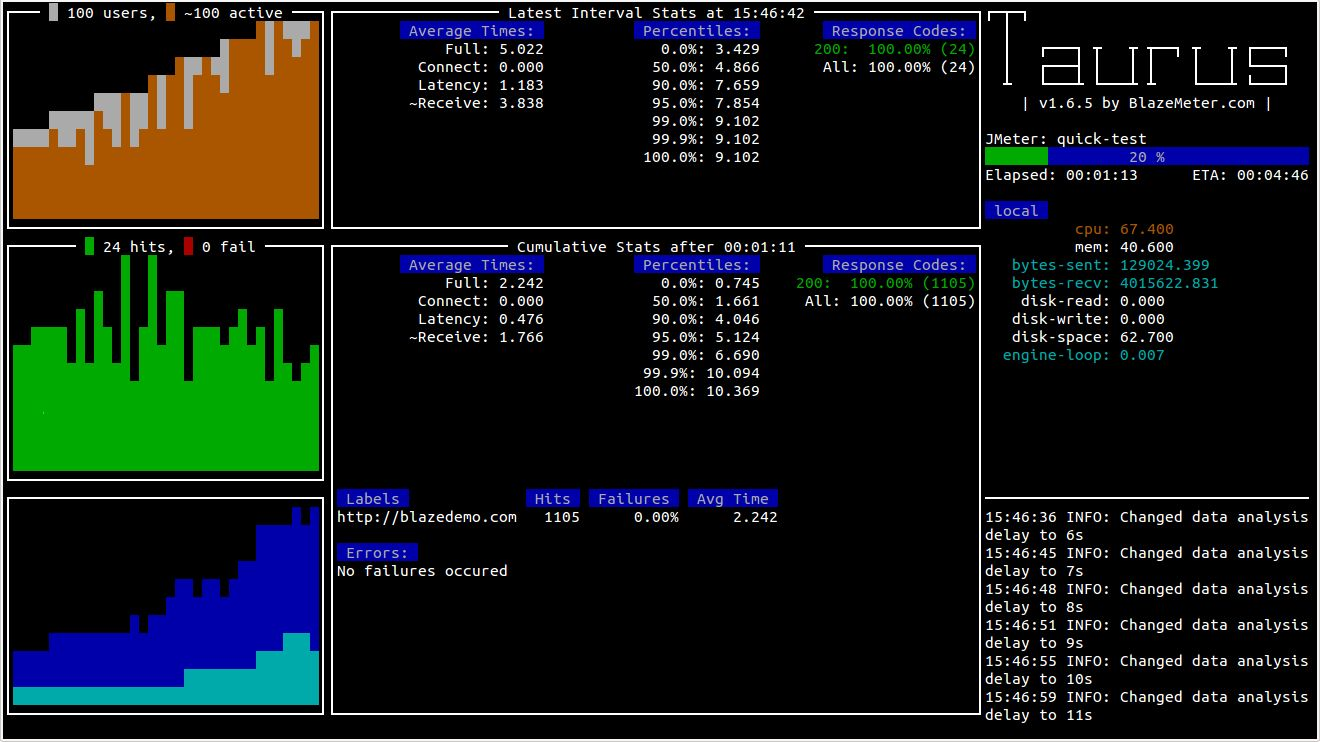
\includegraphics[height=4.5cm]{15_2016_Svirinovski1.png}
\end{figure}

\subsection*{Как это готовить правильно?}

Конфигурационный файл может быть написан на YAML либо JSON. На вышеприведенном примере рассмотрим синтаксис первого из них. Файл должен начинаться с трех дефисов, отступы задают иерархию, основные строительные элементы "--- списки и словари, один элемент структуры на строку. Этих знаний достаточно, чтобы понимать и модифицировать образцы (например, с сайта gettaurus.org).

Приложение консольное, вопросов не задает и сходу встраивается в любую автоматизацию. На это хотелось бы обратить особое внимание: не просто совместимость, но удобство применения, скажем, для Continuous Integration "--- едва ли не основной принцип проекта. Добавлением нескольких строчек возможно:

\begin{itemize}
  \item запустить одновременно несколько генераторов нагрузки;
  \item отложить тест на определенное время;
  \item настроить критерии успешности теста в том числе и на основании полученных http-пакетов;
  \item менять исполнителя "--- например, потребление ресурсов \linebreak JMeter’ом вас не устраивает или нужны возможности \linebreak Selenium’а;
  \item использовать разные типы http-запросов, добавлять заголовки и т.д.;
  \item получить web-отчет, ссылку на который можно отправить коллеге;
  \item перенести тест в облако и выполнить на десятках виртуальных машин (осторожно, это может быть платно, о чем я расскажу ниже).
\end{itemize}

Сейчас мы поддерживаем девять генераторов нагрузки "--- JMeter, Selenium, Gatling, Grinder, Locust, PBench, Siege, Apache Benchmark и Tsung.

Taurus преобразовывает конфигурационные параметры в опции, понятные конкретному генератору. Для JMeter генерируется XML (JMX), для Gatling "--- код на Scala (разумеется, выполнение уже готовых нативных тестовых скриптов также возможно). При необходимости Taurus скачивает инструмент из сети, запускает, следит за работой показывая промежуточные результаты (более или менее в реальном времени) и в конце теста выдает финальный отчет.

Отдельно нужно коснуться некоторых принципов выдачи результатов. 
Данные агрегируются по временным интервалам и выделяются настраиваемыми перцентилями "--- так, например, инженеру будет интересно, уложились ли 98\% запросов в лимит времени. При этом результаты различных инструментов выглядят одинаково и могут сравниваться по основным метрикам.

Ещё пользователь может:

\begin{itemize}
  \item выполнять мониторинг ресурсов как генерующей нагрузку системы, так и нагружаемой "--- очевидно, истощение ресурсов любой из них тестировщику следует знать;
  \item производить быструю настройку переопределяя элементы конфигурации из командной строки;
  \item структурировать тест-план используя включаемые файлы;
  \item определять команды операционной системы для выполнения на разных этапах теста.
\end{itemize}

Для специалистов замечу, что основным поддерживаемым инструментом является JMeter, так уж сложился спрос в индустрии.

\subsection*{Работа изнутри, перспективы}

В данный момент разработка идет силами трех человек программистов. Исходный код публично на Github, поддержка пользователей идет посредством Google Groups. Для контроля качества кода изменения оформляются pullrequest’ами, проходящими обязательное review. Выделенных тестировщиков нету, их роль играет армия пользователей, на сообщения которых мы стараемся реагировать \textbf{безотлагательно}. 
Код основательно покрыт юнит-тестами (на данный момент покрытие составляет 92\%).

Сборку и деплой пакета и сайта Taurus’a осуществляет Jenkins, выполняя перед этим функциональное и unit-тестирование. Для проверки commit’ов используются также Travis и Appveyor. JIR’ы у нас нету, и github’овский issue tracker отключен по вышеупомянутым соображениям "--- основная идея поддержки заключается в том, чтобы исправлять выявленные баги немедленно.

Можно уверенно говорить что мы уже стали полезны "--- в этом году нас почтил вниманием devops.com. Развитие идет достаточно активно, по крайней мере, новый функционал добавляется в планы быстрее, чем реализовывается.

BlazeMeter достаточно ненавязчиво продвигает некоторую интеграцию со своим сервисом "--- как я уже говорил, web-отчеты на их сайте, одна виртуальная машина бесплатно для облачного исполнения, некоторые сложные конвертации форматов.

Основная задача, которую ставит перед нами BlazeMeter "--- делать удобный продукт, который привлечет ощутимую часть сообщества, поэтому многие новые направления вырастают из хотелок пользователей. Из подобных глобальных вещей могу отметить скорый приход поддержки функционального тестирования, валидацию конфигурационных файлов, скоростную фотосъемку загрузки web-страницы, поддержку Selenium-тестов на .Net и JS.

\subsection*{Как мы дошли до такой жизни}

Компания BlazeMeter, зарегистрированная в США и имеющая команду разработки в Израиле, уже около пяти лет предлагает средства для тестирования формата <<поставь галочки на сайте, а мы за тебя создадим нагрузку и покажем отчёт>>.

В поисках новых ниш компания обратила внимание на инженеров. Даже не принося деньги напрямую довольные технически грамотные люди создают очень полезный с точки зрения IT-бизнеса фон, недостижимый, например, рекламой или скидками. Этим клиентам не лень читать документацию, но им нужны очень мощные и гибкие инструменты, а ещё лучше "--- поддержка тех инструментов, которые они уже используют (много ли среди нас желающих переучиваться?). А то, что они используют, оставляет желать лучшего "--- значит, есть где приложить силы и получить хорошую репутацию.

Языком для проекта был выбран Python, отлично подходящий для работы со сторонними инструментами в командной строке на различных архитектурах, лицензией "--- Apache 2.0. Архитектура модульная, многие компоненты вполне могут быть переписаны программистом средней руки (поддержка новых генераторов нагрузки или специфический репортер, скажем, отправляющий \linebreak SMS-сообщения).

Так работает Taurus "--- швейцарский нож для инструментов нагрузочного тестирования, дающий пользователям удобный интерфейс взаимодействия с ними (стараясь при этом не потерять некоторые изюминки отдельных генераторов).

\end{document}

\documentclass[10pt, a5paper]{article}
\usepackage{pdfpages}
\usepackage{parallel}
\usepackage[T2A]{fontenc}
\usepackage{ucs}
\usepackage[utf8x]{inputenc}
\usepackage[polish,english,russian]{babel}
\usepackage{hyperref}
\usepackage{rotating}
\usepackage[inner=2cm,top=1.8cm,outer=2cm,bottom=2.3cm,nohead]{geometry}
\usepackage{listings}
\usepackage{graphicx}
\usepackage{wrapfig}
\usepackage{longtable}
\usepackage{indentfirst}
\usepackage{array}
\newcolumntype{P}[1]{>{\raggedright\arraybackslash}p{#1}}
\frenchspacing
\usepackage{fixltx2e} %text sub- and superscripts
\usepackage{icomma} % коскі ў матэматычным рэжыме
\PreloadUnicodePage{4}

\newcommand{\longpage}{\enlargethispage{\baselineskip}}
\newcommand{\shortpage}{\enlargethispage{-\baselineskip}}

\def\switchlang#1{\expandafter\csname switchlang#1\endcsname}
\def\switchlangbe{
\let\saverefname=\refname%
\def\refname{Літаратура}%
\def\figurename{Іл.}%
}
\def\switchlangen{
\let\saverefname=\refname%
\def\refname{References}%
\def\figurename{Fig.}%
}
\def\switchlangru{
\let\saverefname=\refname%
\let\savefigurename=\figurename%
\def\refname{Литература}%
\def\figurename{Рис.}%
}

\hyphenation{admi-ni-stra-tive}
\hyphenation{ex-pe-ri-ence}
\hyphenation{fle-xi-bi-li-ty}
\hyphenation{Py-thon}
\hyphenation{ma-the-ma-ti-cal}
\hyphenation{re-ported}
\hyphenation{imp-le-menta-tions}
\hyphenation{pro-vides}
\hyphenation{en-gi-neering}
\hyphenation{com-pa-ti-bi-li-ty}
\hyphenation{im-pos-sible}
\hyphenation{desk-top}
\hyphenation{elec-tro-nic}
\hyphenation{com-pa-ny}
\hyphenation{de-ve-lop-ment}
\hyphenation{de-ve-loping}
\hyphenation{de-ve-lop}
\hyphenation{da-ta-ba-se}
\hyphenation{plat-forms}
\hyphenation{or-ga-ni-za-tion}
\hyphenation{pro-gramming}
\hyphenation{in-stru-ments}
\hyphenation{Li-nux}
\hyphenation{sour-ce}
\hyphenation{en-vi-ron-ment}
\hyphenation{Te-le-pathy}
\hyphenation{Li-nux-ov-ka}
\hyphenation{Open-BSD}
\hyphenation{Free-BSD}
\hyphenation{men-ti-on-ed}
\hyphenation{app-li-ca-tion}

\def\progref!#1!{\texttt{#1}}
\renewcommand{\arraystretch}{2} %Іначай формулы ў матрыцы зліпаюцца з лініямі
\usepackage{array}

\def\interview #1 (#2), #3, #4, #5\par{

\section[#1, #3, #4]{#1 -- #3, #4}
\def\qname{LVEE}
\def\aname{#1}
\def\q ##1\par{{\noindent \bf \qname: ##1 }\par}
\def\a{{\noindent \bf \aname: } \def\qname{L}\def\aname{#2}}
}

\def\interview* #1 (#2), #3, #4, #5\par{

\section*{#1\\{\small\rm #3, #4. #5}}

\def\qname{LVEE}
\def\aname{#1}
\def\q ##1\par{{\noindent \bf \qname: ##1 }\par}
\def\a{{\noindent \bf \aname: } \def\qname{L}\def\aname{#2}}
}

\begin{document}
\title{Написание своей StdLibC}
\author{Дмитрий Храбров, Homel, Belarus}
\maketitle
\begin{abstract}
This article shows how you can implement basic stdlib's functions. You can see here: string functions, formatted output, usage of *Nix kernel functions etc.
\end{abstract}
В последнее время на страницах информационных ресурсов можно увидеть статьи <<Привет из свободного от libc мира>> ~\cite{Khrabrov1}, <<Минимальный Elf>> ~\cite{Khrabrov2} и пр. Все они показывают настройку получаемого исполняемого файла, стараются его уменьшить. Например, получен работающий Elf-файл, занимающий всего 45 байт дискового пространства. Однако за данной минимизацией забывается такое важное свойство, как юзабилити. Elf-файл в 45 байт умеет только запускаться и корректно завершаться. При этом если добавить хотя бы вывод классического сообщения <<Hello World>>, то размер станет далеко не таким маленьким и от многих техник придётся отказаться.

Существует множество свободных реализаций стандартной библиотеки Си ~\cite{Khrabrov3}. Минимальный размер имеет dietlibc, которая позволяет скомпилировать приложение размером всего 200 байт. Или 6 килобайт если используется функция printf. Однако значительная часть функционала там не реализована, или реализована не в соответствии со стандартом. Кроме того, dietlibc лицензирована под GPL2, что ставит ряд значительных ограничений (свои приложения придётся так же лицензировать под GPL2). Ещё одной хорошей альтернативой в плане размера является musl: 1800 байт минимум, 13 килобайт с printf. Библиотека musl лицензирована под MIT и качественно реализует стандарт. Однако именно из-за полного охвата стандарта Си и получаются 13 килобайт, которые хотелось бы уменьшить.

Целью данной работы является создание библиотеки, с помощью которой можно было бы более-менее привычно программировать, но в то же время минимизировать размер получаемого исполняемого файла, вообще не использовать стандартную библиотеку. Данная работа представляет больше исследовательский интерес, чем практическую ценность. И в конечном счёте приближает к пониманию, как именно работают те или иные функции из стандартной библиотеки языка Си. Предложенные реализации далеко не оптимальны или безопасны, однако просты для понимания.

В итоге необходимо получить корректное функционирование \linebreak данного кода:
\lstset{ %
language=C,                 % выбор языка для подсветки (здесь это С)
basicstyle=\small\sffamily, % размер и начертание шрифта для подсветки кода
breaklines=true,           % автоматически переносить строки (да\нет)
breakatwhitespace=false, % переносить строки только если есть пробел
}
\begin{lstlisting}
printf("Hello %s LVEE %d!\n", "Summer", 2016);
\end{lstlisting}

В этой простейшей, казалось бы, строке кода, поднимается сразу несколько вопросов: 1) непосредственно сама функция printf и её форматный вывод; 2) функции работы со строками; 3) конвертирование чисел в строку; 4) непосредственно вывод символов на экран. Всё это обычно реализуется средствами стандартной библиотеки, и всё придётся реализовать самостоятельно.

Syscall "--- вызов функций ядра Linux, для x86 реализуется через $0\times80$ ассемблерное прерывание. Полный код для функции с 3 аргументами (взят из ~\cite{Khrabrov4}):

\begin{lstlisting}
static long _syscall3(int number, unsigned long arg1, unsigned long arg2, unsigned long arg3){
  long result;
    __asm__ volatile ("int $0x80"
    : "=a" (result)
    : "0" (number), "b" (arg1), "c" (arg2), "d" (arg3)
    : "memory", "cc");
  return result;
}
\end{lstlisting}

Если вызываемой функции необходимо менее 3 аргументов, то завершающие аргументы можно передать нулевыми. Например, \linebreak функция close принимает всего 1 аргумент "--- файловый дескриптор. Реализация может выглядеть следующим образом:

\begin{lstlisting}
return (int)syscall3(__NR_close, fd, 0, 0);
\end{lstlisting}

Константы названий функций (NR\_close и пр.) задаются для каждой архитектуры отдельно в файле unistd.h. Это заголовочный файл для доступа к API POSIX-совместимой операционной системы. В unistd.h можно посмотреть полный список функций ядра Linux. И не увидеть там ни строковых функций, ни потоков (thread), ни malloc/calloc/free, ни printf. Весь этот функционал реализуется на функциях более низкого уровня в стандартной библиотеке. Вывод символов на экран консоли осуществляется с помощью функции write:

\begin{lstlisting}
return (ssize_t)syscall3(__NR_write, fd, buf, count);
\end{lstlisting}

Как видно, функция write использует 3 аргумента: файловый дескриптор, буфер и размер буфера в байтах. Однако бывают ситуации, когда размер буфера заранее неизвестен. Обычно в таких случаях используется функция получения длины строки "--- strlen. Реализуется она средствами чистого Си, без вызова функций ядра. Это является преимуществом, так как такой код может быть скомпилирован любым компилятором, реализующим стандарт Си. Начиная от свободных GCC, Clang, Tiny C Compiler, и заканчивая проприетарной Visual Studio. Пример реализации поиска длины строки:

\begin{lstlisting}
len=0; while( str[len] != 0 ) len++;
\end{lstlisting}

Аналогично реализуются и многие другие функции работы со строками "--- происходит посимвольная обработка всей строки в цикле. В качестве примера обработки одного символа можно рассмотреть функцию перевода символа в верхний регистр. Если символ лежит в интервале от a до z, то от его кода отнимается <<a>> и прибавляется код <<A>>:

\begin{lstlisting}
return symb - 'a' + 'A';
\end{lstlisting}

Конвертирование целых чисел в строку "--- деление на 10 до тех пор, пока не останется 0. Остаток от деления складывать в буфер. Существует множество способов сделать перевод из числа в строку, но они всё-равно опираются на какой-либо один базовый, который и необходимо реализовать.

Функция printf может принимать разное количество аргументов. Эта <<перегрузка>> параметров функции осуществляется средствами Си через списки варьирующихся аргументов: va\_list, \linebreak va\_start, va\_arg, va\_end.

Пример реализации:

\begin{verbatim}
void Myprintf(char* format, ...){
  char* s;  // Буфер для вывода строк 
  int i; // Счётчик текущей позиции в форматной строке
  va_list arg; // Список варьирующихся аргументов
  va_start(arg, format); // Инициализируем список
  for(i=0; i<strlen(format); i++){
    if( format[i] == '%' ) switch( format[i+1] ){
      case 'd': // вызов своей функции для чисел
        MyPutInt( va_arg(arg, int) ); i++; break;
      case 's': // получение строки и её вывод
        s = va_arg(arg, char*);  
        MyWrite( s, strlen(s) ); i++; break;
      case 'c': // аргумент - в int
        MyPutchar( va_arg(arg, int) ); i++; break;
    } else MyPutchar( format[i] );
  } // вывод одного символа реализуется через write
  va_end(arg); // Необходимая очистка списка
}
\end{verbatim}

Суть так же проста "--- перебираем символы форматной строки, если встречаем символ `\%', то смотрим следующий за ним. По следующему символу узнаём тип аргумента (если символ <<d>>, то нужно конвертировать в int). Далее просто берём следующий аргумент из списка варьируемых, сразу просим привести его к нужному типу. Нужно помнить, что нельзя сразу конвертировать во float, char или short "--- изначально должно быть преобразование в double или int.

Теперь остаётся только скомпилировать приложение с флагами nodefaultlibs и nostartfiles (подробнее про это можно почитать в статье <<Привет из свободного от libc мира>> ~\cite{Khrabrov1}). Если всё собрано правильно, то при вызове ldd будет писать <<not a dynamic executable>>. Это означает, что полученное приложение вообще не зависит ни от каких системных библиотек. Но в то же время оно написано на Си и использует функцию printf, что и требовалось получить.

\begin{thebibliography}{99}

\bibitem{Khrabrov1} Hello from a libc-free world! \url{https://blogs.oracle.com/ksplice/entry/hello\_from\_a\_libc\_free}
\bibitem{Khrabrov2} A Whirlwind Tutorial on Creating Really Teensy ELF Executables for Linux. \url{http://www.muppetlabs.com/\~{}breadbox/software/tiny/teensy.html}
\bibitem{Khrabrov3} Comparison of C/POSIX standard library implementations for Linux. \url{http://www.etalabs.net/compare\_libcs.html}
\bibitem{Khrabrov4} Program in C without any C library. \url{https://github.com/fishilico/shared/tree/master/linux/nolibc}
\end{thebibliography}
\end{document}

\documentclass[10pt, a5paper]{article}
\usepackage{pdfpages}
\usepackage{parallel}
\usepackage[T2A]{fontenc}
\usepackage{ucs}
\usepackage[utf8x]{inputenc}
\usepackage[polish,english,russian]{babel}
\usepackage{hyperref}
\usepackage{rotating}
\usepackage[inner=2cm,top=1.8cm,outer=2cm,bottom=2.3cm,nohead]{geometry}
\usepackage{listings}
\usepackage{graphicx}
\usepackage{wrapfig}
\usepackage{longtable}
\usepackage{indentfirst}
\usepackage{array}
\newcolumntype{P}[1]{>{\raggedright\arraybackslash}p{#1}}
\frenchspacing
\usepackage{fixltx2e} %text sub- and superscripts
\usepackage{icomma} % коскі ў матэматычным рэжыме
\PreloadUnicodePage{4}

\newcommand{\longpage}{\enlargethispage{\baselineskip}}
\newcommand{\shortpage}{\enlargethispage{-\baselineskip}}

\def\switchlang#1{\expandafter\csname switchlang#1\endcsname}
\def\switchlangbe{
\let\saverefname=\refname%
\def\refname{Літаратура}%
\def\figurename{Іл.}%
}
\def\switchlangen{
\let\saverefname=\refname%
\def\refname{References}%
\def\figurename{Fig.}%
}
\def\switchlangru{
\let\saverefname=\refname%
\let\savefigurename=\figurename%
\def\refname{Литература}%
\def\figurename{Рис.}%
}

\hyphenation{admi-ni-stra-tive}
\hyphenation{ex-pe-ri-ence}
\hyphenation{fle-xi-bi-li-ty}
\hyphenation{Py-thon}
\hyphenation{ma-the-ma-ti-cal}
\hyphenation{re-ported}
\hyphenation{imp-le-menta-tions}
\hyphenation{pro-vides}
\hyphenation{en-gi-neering}
\hyphenation{com-pa-ti-bi-li-ty}
\hyphenation{im-pos-sible}
\hyphenation{desk-top}
\hyphenation{elec-tro-nic}
\hyphenation{com-pa-ny}
\hyphenation{de-ve-lop-ment}
\hyphenation{de-ve-loping}
\hyphenation{de-ve-lop}
\hyphenation{da-ta-ba-se}
\hyphenation{plat-forms}
\hyphenation{or-ga-ni-za-tion}
\hyphenation{pro-gramming}
\hyphenation{in-stru-ments}
\hyphenation{Li-nux}
\hyphenation{sour-ce}
\hyphenation{en-vi-ron-ment}
\hyphenation{Te-le-pathy}
\hyphenation{Li-nux-ov-ka}
\hyphenation{Open-BSD}
\hyphenation{Free-BSD}
\hyphenation{men-ti-on-ed}
\hyphenation{app-li-ca-tion}

\def\progref!#1!{\texttt{#1}}
\renewcommand{\arraystretch}{2} %Іначай формулы ў матрыцы зліпаюцца з лініямі
\usepackage{array}

\def\interview #1 (#2), #3, #4, #5\par{

\section[#1, #3, #4]{#1 -- #3, #4}
\def\qname{LVEE}
\def\aname{#1}
\def\q ##1\par{{\noindent \bf \qname: ##1 }\par}
\def\a{{\noindent \bf \aname: } \def\qname{L}\def\aname{#2}}
}

\def\interview* #1 (#2), #3, #4, #5\par{

\section*{#1\\{\small\rm #3, #4. #5}}

\def\qname{LVEE}
\def\aname{#1}
\def\q ##1\par{{\noindent \bf \qname: ##1 }\par}
\def\a{{\noindent \bf \aname: } \def\qname{L}\def\aname{#2}}
}

\begin{document}
\title{<<Параноидальный>> офис "---  оборотная сторона безопасности\footnote{\url{admin@itg.by}, \url{http://lvee.org/ru/abstracts/206}}}
\author{Дмитрий Степанов, Минск, Беларусь}
\maketitle
\begin{abstract}
News about data breaches, hacking, discovered vulnerabilities are now typical. Common solutions deal with external threats along with international standards and best practices, not taking into account non-commercial threats of information leaks.
\end{abstract}
С каждым годом информационные ресурсы и системы развиваются, все глубже проникают в повседневную деятельность компаний и каждого человека в отдельности. Сейчас ни у кого не вызывает удивления новость об утечке данных пользователей того или иного сервиса, взломе системы, обнаружении уязвимости продукта. Многие руководители предприятий полагают, что это их не коснется, так как <<это где-то там, а мы здесь>>. Решения, внедряемые на предприятиях, защищают в большинстве от внешних угроз, взломов, атак, они согласованы с международными стандартами и рекомендациями (cobit, itil и т. д.), и в большинстве своем оценивают риски потери информации с точки зрения  убытков для предприятия, но не учитывают, что информация на предприятии может быть не только коммерческой но и чрезмерно конфиденциальной в ином плане.

Весь этот информационный поток порождает у руководителей частных предприятий вполне обоснованную паранойю о сохранности информации по деятельности предприятия.

Исходя из выше описанного мы и рассмотрим распространившуюся паранойю одного руководителя частной компании <<X>>  и реализацию его желаний и потребностей.

На момент созревания <<wish list>> система компании <<X>> представляла собой филиальную сеть между двумя странами, граничащими друг с другом. В стране <<А>> находился отдел продажи и маркетинга (собственно, мы находились в стране <<А>>), а в стране <<Б>> "--- производство, логистика и небольшие продажи.

\textbf{Инфраструктура} была реализована на основе платного ПО (все лицензировано) и представляла следующую картину:

\begin{itemize}
  \item 80 ПК с установленными операционными системами Windows;
  \item 3 Сервера: 1. Шлюз на платном ПО; 2. Бухгалтерия на платном ПО; 3. Файловый сервер на Платном ПО.
\end{itemize}

Структура описана кратко и не учитывает наличие АТС и структуры сети (наличия коммутационного оборудования и Wi-fi точек).

\subsection*{Задача.}

Была поставлена задача реализовать полное шифрование каналов связи с внешним миром, шифрование почтовой переписки, отслеживание сотрудников, максимально ограничить возможность утечки информации через сотрудников компании и в случае <<случайной пропажи какого-либо сервера или компьютера с жесткими дисками из компании>>. Важнейшим условием стало уменьшение стоимости лицензирования ПО и то, что внедряемый проект в последующем будет распространен на остальные подразделения компании.

\subsection*{План создания.}

Выбор ОС пал на дистрибутивы Linux по следующим причинам:

\begin{itemize}
  \item низкий уровень владения и грамотности конечных пользователей в среде Linux;
  \item стоимость дистрибутива Linux;
  \item возможность реализации шифрования из коробки;
  \item наличие альтернативного ПО на замену проприетарным пакетам в среде Windows;
  \item компания занимается продажами "--- количество узкоспециализированного по незначительного;
  \item производительность ОС на разношерстном парке ПК.
\end{itemize}

В результате сервера были реализованы на Ubuntu Linux, а клиентские места на Linux Mint Xfce Edition.

\subsection*{Защита каналов и выбор шлюза.}

Реализация защиты каналов была проведена посредством объединения филиалов Ipsec тоннелем, в качестве межсетевого экрана тестирровались системы Zentyal и ZeroShell. В городе <<А>> был установлен ZeroShell благодаря его возможности работать с LiveCD. На второй стороне в городе <<Б>> был установлен Zentyal "--- использовался как почтовый сервер и LDAP-сервер. Оба сервера работают под приложением OpenVPN, и таким образом реализация тоннеля не вызвала каких-либо существенных трудностей.

Маршруты были настроены так, что весь офис <<А>> выходит в интернет через офис <<Б>>. Также был реализован отдельный канал IPSec с SIP-провайдером посредством установки маршрутизатора на стороне провайдера.

В последствии система несколько видоизменялась в связи с улучшением интеграции.

Почтовая переписка была переведена на почтовый клиент \linebreak Thunderbird c реализованным модулем шифрования на основе PGP. На всех ПК был настроен Iptables для работы только в конкретной сети и с конкретными портами.

\subsection*{Шифрование серверов и офисного ПК.}

Полное шифрование диска (Full Disk Encryption, FDE) стало доступнее для простых пользователей Linux. Так начиналась статья (откровенно говоря, не помню какого журнала и тем более автора), ставшая в свое время основой для неоднократной реализации <<параноидальных офисов>>.

По очевидным причинам, мы не хотели стать жертвами \linebreak термально-ректального криптоанализа со стороны злоумышленников, в результате чего выбрали Luks-шифрование с использованием ключей на основе сертификатов, причем сертификат находился за пределами границ государства офиса <<А>>. Также были предприняты меры по уничтожению сертификата в случае необходимости сохранения информации в безопасности.

Контроль целостности файловой структуры был реализован посредством программного модуля Tripwire.

Таким образом мы получили полностью реализованную на \linebreak GNU/Linux структуру с шифрованием дисков, на которых оставалась исключительно загрузочная область для получения сертификата и разблокирования диска.

\subsection*{Реализация отслеживания персонала.}

Данный вопрос решился на удивление просто: у каждого сотрудника существовал корпоративный телефон на Android или iPhone, который проходил перед каждой командировкой подготовку и чистку у отдела IT. На данные аппараты были установлены скрытые приложения для программного СПО Traccar. Это позволило убить сразу двух зайцев: контроль транспорта и командированных сотрудников, так как телефоны были заведены через VPN-канал на АТС для осуществления звонков через SIP и бесплатной связи с офисом, отключения производились редко, и в результате трек и местоположение были корректны и отчетливы.

Для реализации удаленной работы и подачи приложений (с почтой и иными приложениями) на случай необходимости был рассмотрен продукт Ulteo, недостатком которого было использование Java, но переход на HTML5 вопросы снял.

\subsection*{Подводя итоги:}

Реализация данного проекта позволила в очередной раз пользователям с иной стороны рассмотреть СПО. Экономическая выгода, а так же явное преимущество <<коробочного решения>> по шифрованию, альтернативное офисное ПО и уровень защищенности платформы (благодаря низкой пользовательской популярности и своей структуре) от внешнего зловредного ПО делают гибридные интеграционные решения все более востребованными в современном мире.

\end{document}

\documentclass[10pt, a5paper]{article}
\usepackage{pdfpages}
\usepackage{parallel}
\usepackage[T2A]{fontenc}
\usepackage{ucs}
\usepackage[utf8x]{inputenc}
\usepackage[polish,english,russian]{babel}
\usepackage{hyperref}
\usepackage{rotating}
\usepackage[inner=2cm,top=1.8cm,outer=2cm,bottom=2.3cm,nohead]{geometry}
\usepackage{listings}
\usepackage{graphicx}
\usepackage{wrapfig}
\usepackage{longtable}
\usepackage{indentfirst}
\usepackage{array}
\newcolumntype{P}[1]{>{\raggedright\arraybackslash}p{#1}}
\frenchspacing
\usepackage{fixltx2e} %text sub- and superscripts
\usepackage{icomma} % коскі ў матэматычным рэжыме
\PreloadUnicodePage{4}

\newcommand{\longpage}{\enlargethispage{\baselineskip}}
\newcommand{\shortpage}{\enlargethispage{-\baselineskip}}

\def\switchlang#1{\expandafter\csname switchlang#1\endcsname}
\def\switchlangbe{
\let\saverefname=\refname%
\def\refname{Літаратура}%
\def\figurename{Іл.}%
}
\def\switchlangen{
\let\saverefname=\refname%
\def\refname{References}%
\def\figurename{Fig.}%
}
\def\switchlangru{
\let\saverefname=\refname%
\let\savefigurename=\figurename%
\def\refname{Литература}%
\def\figurename{Рис.}%
}

\hyphenation{admi-ni-stra-tive}
\hyphenation{ex-pe-ri-ence}
\hyphenation{fle-xi-bi-li-ty}
\hyphenation{Py-thon}
\hyphenation{ma-the-ma-ti-cal}
\hyphenation{re-ported}
\hyphenation{imp-le-menta-tions}
\hyphenation{pro-vides}
\hyphenation{en-gi-neering}
\hyphenation{com-pa-ti-bi-li-ty}
\hyphenation{im-pos-sible}
\hyphenation{desk-top}
\hyphenation{elec-tro-nic}
\hyphenation{com-pa-ny}
\hyphenation{de-ve-lop-ment}
\hyphenation{de-ve-loping}
\hyphenation{de-ve-lop}
\hyphenation{da-ta-ba-se}
\hyphenation{plat-forms}
\hyphenation{or-ga-ni-za-tion}
\hyphenation{pro-gramming}
\hyphenation{in-stru-ments}
\hyphenation{Li-nux}
\hyphenation{sour-ce}
\hyphenation{en-vi-ron-ment}
\hyphenation{Te-le-pathy}
\hyphenation{Li-nux-ov-ka}
\hyphenation{Open-BSD}
\hyphenation{Free-BSD}
\hyphenation{men-ti-on-ed}
\hyphenation{app-li-ca-tion}

\def\progref!#1!{\texttt{#1}}
\renewcommand{\arraystretch}{2} %Іначай формулы ў матрыцы зліпаюцца з лініямі
\usepackage{array}

\def\interview #1 (#2), #3, #4, #5\par{

\section[#1, #3, #4]{#1 -- #3, #4}
\def\qname{LVEE}
\def\aname{#1}
\def\q ##1\par{{\noindent \bf \qname: ##1 }\par}
\def\a{{\noindent \bf \aname: } \def\qname{L}\def\aname{#2}}
}

\def\interview* #1 (#2), #3, #4, #5\par{

\section*{#1\\{\small\rm #3, #4. #5}}

\def\qname{LVEE}
\def\aname{#1}
\def\q ##1\par{{\noindent \bf \qname: ##1 }\par}
\def\a{{\noindent \bf \aname: } \def\qname{L}\def\aname{#2}}
}

\begin{document}
\title{Технология прозрачного сжатия графической памяти GPU\footnote{\url{rogachevsergei@gmail.com}, \url{http://lvee.org/ru/abstracts/216}}}
\author{Сергей Рогачев, Москва, Russian Federation}
\maketitle
\begin{abstract}
Complexity of graphical user interfaces of mobile applications is growing rapidly. Much memory is needed to keep buffers for textures and graphical data. Modern mobile GPUs do not have built-in memory and use general memory to keep graphic buffers. A part of RAM is occupied by GPU and cannot be used by an operating system. According to this research most of such buffers are well compressible: 6-9 times. We propose a technology for transparent compression of graphic buffers in Linux kernel.
\end{abstract}
Каждый год анонсируются новые, все более совершенные гаджеты, использующие ядро Linux и открытые платформы: планшеты, смартфоны, телевизионные приставки, умные часы. Большинство из них оснащается мобильными GPU, используемыми для аппаратного ускорения 3D графики (OpenGL ES) и параллельных вычислений (OpenCL, RenderScript). Наиболее часто встречаются графические процессоры Mali, Adreno и PowerVR. В отличие от GPU, используемых в настольных системах, мобильные GPU не имеют встроенной памяти, а используют часть оперативной (рис. ~\ref{Rogachev1}), предоставляемой ядром ОС "--- такая память становится недоступной ядру ОС и пользовательским программам. Будем называть память, используемую GPU, графической памятью. Оптимизация расхода такой памяти позволит достичь снижения цены устройств или повысить производительность за счет улучшения кешируемости приложений.

\begin{figure}[h!]
  \centering
  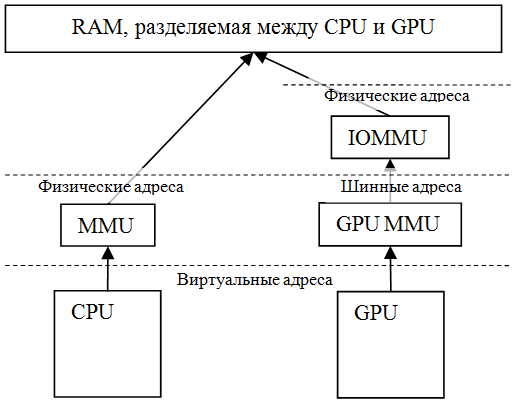
\includegraphics[]{18_2016_Rogachev1.png}
  \caption{Разделение памяти между CPU и GPU}
  \label{Rogachev1}
\end{figure}

К графической памяти можно отнести GEM буферы, используемые для хранения результата рендеринга, и вспомогательные регионы (native буферы), хранящие цветовые буферы, поверхности, текстуры, различную вспомогательную информацию, относящуюся к элементам графической сцены.

Задача оптимизации использования графической памяти уже рассматривалась ранее ~\cite{Rogachev1}, в статье упоминалась технология сжатия GEM буферов на стороне пользователя, также были отмечены высокие накладные расходы этого решения.

В настоящей работе рассматривается исключительно вопрос оптимизации использования native буферов, поскольку современные композитные менеджеры уже способны эффективно управлять \linebreak GEM буферами и дальнейшая работа в этом направлении не требуется.

Авторами было проведено исследование вопроса на примере \linebreak GPU Mali серий Midgard и Utgard: за счет доработки драйверов ядра удалось реализовать прозрачную компрессию редко используемых native буферов графической памяти. В результате получилось добиться экономии более 100 Мб. оперативной памяти за счет высокого коэффициента сжатия графических буферов (6 "--- 9 раз), а также наличия множества регионов графической памяти, заполненных нулями.

По своей сути решение реализует механизм схожий с подкачкой страниц (swap), при этом есть ряд особенностей, характерных для графической памяти и мобильных устройств. Ранее подобный подход рассматривался как трудно реализуемый ~\cite{Rogachev2}.

Для сжатия некоторого региона графической памяти нужна гарантия, что он не будет использоваться CPU или GPU в процессе компрессии. Это гарантируется путем запрета доступа к страницам данного региона в таблицах страниц GPU, а также снятия отображений региона в адресные пространства процессов на CPU. После того, как соответствующие записи PTE и ATE (записи таблиц страниц CPU и GPU, соответственно) изменены, любое обращение к соответствующим адресам памяти должно вызвать исключение страничной адресации, известное как page fault или data abort.

После того как гарантировано отсутствие доступа к региону памяти, данные со страниц этого региона могут быть сжаты, а страницы освобождены. Для хранения сжатых данных графической памяти в работе применена подсистема GMC (graphical memory compression), созданная в качестве обобщенного слоя для разных драйверов GPU. GMC осуществляет управление буферами для хранения сжатых данных через подсистему ядра zpool (zsmalloc \linebreak allocator ~\cite{Rogachev3}), сжатие данных с использованием crypto comp API, управление идентификаторами сжатых страниц, а также контролирует когерентность кешей. Страницы, данные которых плохо сжимаются, не принимаются для хранения и не освобождаются. Страницы, заполненные нулями, учитываются GMC и освобождаются.

При обращении к адресам страниц графической памяти, освобожденной ранее, генерируются исключения страничной адресации.  Соответствующие данные извлекаются из хранилища GMC на вновь выделенные страницы физической памяти. Осуществляется отображение новых страниц по требуемым виртуальным адресам путем изменения записей PTE или ATE в соответствующих таблицах страниц.

Кроме уже описанного механизма важным является вопрос о ранжировании регионов графической памяти по признаку частоты доступа. Сжатие активно используемой памяти может привести к катастрофическому падению производительности за счет частых исключений страничной адресации. Для решения указанной проблемы используется информация о состоянии приложений. Специальный демон (resource daemon) следит за приложениями и информирует ядро о тех из них, которые переходят в фоновый режим (становятся невидимыми на экране). Графическая память таких приложений подлежит сжатию.

Взаимодействие всех компонент во время компрессии отражено на рис. ~\ref{Rogachev2}. Основные шаги пронумерованы.

\begin{figure}[h!]
  \centering
  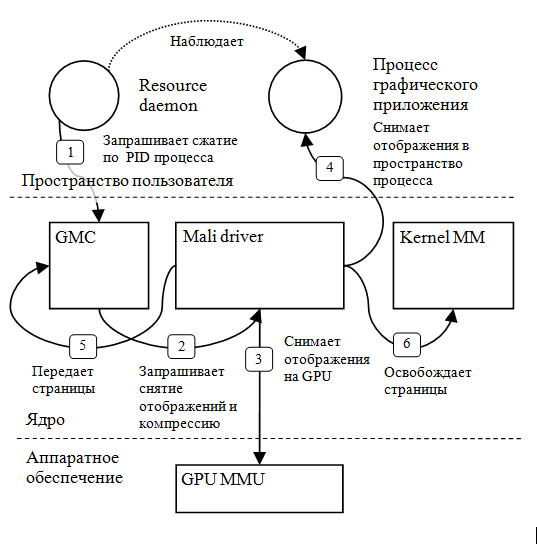
\includegraphics[width=10cm]{18_2016_Rogachev2.png}
  \caption{Взаимодействие компонент системы}
  \label{Rogachev2}
  
\end{figure}

Рис. ~\ref{Rogachev3} иллюстрирует снятие отображений, компрессию и освобождение страниц с позиции данных, а не потока управления и дополняет рис. ~\ref{Rogachev2}.

\begin{figure}[h!]
  \centering
  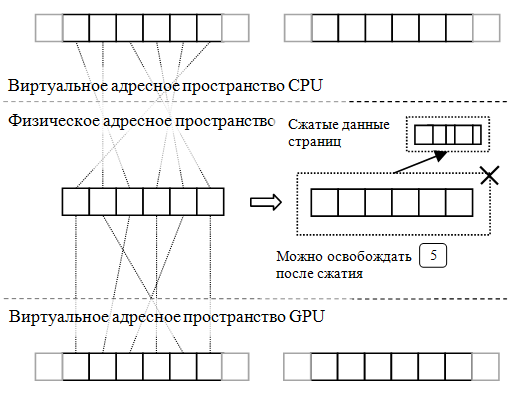
\includegraphics[width=10cm]{18_2016_Rogachev3.png}
  \caption{Снятие отображений и компрессия}
  \label{Rogachev3}
\end{figure}

Тестирование решения на платформах Android и Tizen показало сокращение используемой памяти "--- более 100 мегабайт может быть освобождено при стандартном использовании устройства, когда в фоне оказывается достаточное количество кешированных приложений. Замечено большое количество регионов, заполненных нулями, а максимальная степень сжатия данных графических буферов составила 89\%. Накладные расходы, вносимые решением минимальны, а пиковые не превышают 18\% (Kindle App, Google Maps). В определенных ситуациях переключение между приложениями ускоряется до 40\% за счет большего количества свободной памяти, а следовательно, лучшей кешируемости приложений.

Исходный код подсистемы GMC планируется опубликовать в LKML, а изменения в драйверах Mali через группы поддержки ARM.

\begin{thebibliography}{99}
\bibitem{Rogachev1} Kwon, S., Kim, S.-H., Kim, J.-S., and Jeong, J. Managing gpu buffers for caching more apps in mobile systems. Proceeding EMSOFT '15, 207–216 (2015)
\bibitem{Rogachev2} Carmack, J. GPU data paging, \url{http://media.armadilloaerospace.com/misc/gpuDataPaging.htm} (2010)
\bibitem{Rogachev3} Corbet J. The ZsmallocAllocator. Linux Weekly News (2012)
\end{thebibliography}
\end{document}

\documentclass[10pt, a5paper]{article}
\usepackage{pdfpages}
\usepackage{parallel}
\usepackage[T2A]{fontenc}
\usepackage{ucs}
\usepackage[utf8x]{inputenc}
\usepackage[polish,english,russian]{babel}
\usepackage{hyperref}
\usepackage{rotating}
\usepackage[inner=2cm,top=1.8cm,outer=2cm,bottom=2.3cm,nohead]{geometry}
\usepackage{listings}
\usepackage{graphicx}
\usepackage{wrapfig}
\usepackage{longtable}
\usepackage{indentfirst}
\usepackage{array}
\newcolumntype{P}[1]{>{\raggedright\arraybackslash}p{#1}}
\frenchspacing
\usepackage{fixltx2e} %text sub- and superscripts
\usepackage{icomma} % коскі ў матэматычным рэжыме
\PreloadUnicodePage{4}

\newcommand{\longpage}{\enlargethispage{\baselineskip}}
\newcommand{\shortpage}{\enlargethispage{-\baselineskip}}

\def\switchlang#1{\expandafter\csname switchlang#1\endcsname}
\def\switchlangbe{
\let\saverefname=\refname%
\def\refname{Літаратура}%
\def\figurename{Іл.}%
}
\def\switchlangen{
\let\saverefname=\refname%
\def\refname{References}%
\def\figurename{Fig.}%
}
\def\switchlangru{
\let\saverefname=\refname%
\let\savefigurename=\figurename%
\def\refname{Литература}%
\def\figurename{Рис.}%
}

\hyphenation{admi-ni-stra-tive}
\hyphenation{ex-pe-ri-ence}
\hyphenation{fle-xi-bi-li-ty}
\hyphenation{Py-thon}
\hyphenation{ma-the-ma-ti-cal}
\hyphenation{re-ported}
\hyphenation{imp-le-menta-tions}
\hyphenation{pro-vides}
\hyphenation{en-gi-neering}
\hyphenation{com-pa-ti-bi-li-ty}
\hyphenation{im-pos-sible}
\hyphenation{desk-top}
\hyphenation{elec-tro-nic}
\hyphenation{com-pa-ny}
\hyphenation{de-ve-lop-ment}
\hyphenation{de-ve-loping}
\hyphenation{de-ve-lop}
\hyphenation{da-ta-ba-se}
\hyphenation{plat-forms}
\hyphenation{or-ga-ni-za-tion}
\hyphenation{pro-gramming}
\hyphenation{in-stru-ments}
\hyphenation{Li-nux}
\hyphenation{sour-ce}
\hyphenation{en-vi-ron-ment}
\hyphenation{Te-le-pathy}
\hyphenation{Li-nux-ov-ka}
\hyphenation{Open-BSD}
\hyphenation{Free-BSD}
\hyphenation{men-ti-on-ed}
\hyphenation{app-li-ca-tion}

\def\progref!#1!{\texttt{#1}}
\renewcommand{\arraystretch}{2} %Іначай формулы ў матрыцы зліпаюцца з лініямі
\usepackage{array}

\def\interview #1 (#2), #3, #4, #5\par{

\section[#1, #3, #4]{#1 -- #3, #4}
\def\qname{LVEE}
\def\aname{#1}
\def\q ##1\par{{\noindent \bf \qname: ##1 }\par}
\def\a{{\noindent \bf \aname: } \def\qname{L}\def\aname{#2}}
}

\def\interview* #1 (#2), #3, #4, #5\par{

\section*{#1\\{\small\rm #3, #4. #5}}

\def\qname{LVEE}
\def\aname{#1}
\def\q ##1\par{{\noindent \bf \qname: ##1 }\par}
\def\a{{\noindent \bf \aname: } \def\qname{L}\def\aname{#2}}
}

\switchlang{en}
\begin{document}
\title{First steps into OpenStack\footnote{\url{perepiolkin@itspartner.net}, \url{http://lvee.org/ru/abstracts/217}}}
\author{Andrei Perapiolkin, Minsk, Belarus}
\maketitle
\begin{abstract}
This report aims to give understanding of what OpenStack is, moreover to guide on how to start to use and contribute to the OpenStack. I will describe OpenStack in the context of distributed computing; give short description of OpenStack services Nova, Neutron, Cinder, Swift, Glance, Horisont, Keystone; give short description of devstack, packstack, suseCloud, ubuntu juju. On the example of the devstack, I will give a short description of how you can deploy your own OpenStack cloud.
\end{abstract}


New technologies in the IT world mostly appear on the basis of existing knowledge approaches and infrastructure. It is also true for the cloud computing. We can see that new step of evolution of the grid and cluster systems is Cloud Computing systems. The reason of evolution is high demand for the available computing resources in the society. Rapidly changing modern world requires fast speed deployment of the IT infrastructure. This determines fast deployment of business infrastructure -- fast accessibility to the computing resources, storage, ready software deployments, and others. From the perspective of the people who offer all of these resources it is extremely important to have orchestration tools to control and automate all of these tasks. So the merger of all of the requirements leaded to the appearance of the OpenStack.

OpenStack is a merge of some already existing technologies under the hood of Python automation. It includes such components like:

\begin{itemize}
  \item \textbf{Keystone} provides an authentication and authorization service for other OpenStack services. Provides a catalog of endpoints for all OpenStack services.
  \item \textbf{Nova} manages the computational resources by creating virtual computation environments.
  \item \textbf{Neutron} enables network connectivity for the OpenStack services. It allows to define networks, their topology, and attach instances.
  \item \textbf{Cinder} provides persistent block storage to running instances.
  \item \textbf{Glance} stores images for the Nova. Allowing it to make quick start from prepared image deployment.
  \item \textbf{Swift} stores and retrieves arbitrary unstructured data objects via REST API.
  \item \textbf{Horison} service provides web-based interface, and allows to \linebreak interact with OpenStack services like Cinder, Nova…
\end{itemize}

\begin{figure}[h!]
  \centering
  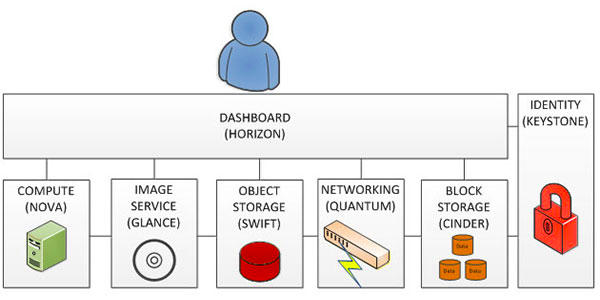
\includegraphics[width=9cm]{19_2016_Perapiolkin1.png}
\end{figure}

There are also such services like \textbf{Ceilometer} (provides telemetry), \textbf{Trove} (interaction with database), \textbf{Manila} (provides shared file \linebreak system) and some others…

For instance, \textbf{Nova} which serves as a computational resource \linebreak provider by itself is a management that aggregates emulation, \linebreak visualization and containerization solutions under the unified API. Nova works with KVM, QEMU, Vmware ESXi, Microsoft Hyper-V, \linebreak XenServer, Docker and others.

Сore OpenStack service deployment process is a complex  task. In bare OpenStack deployment it’s get done by consistent configuration of each servicein in the manner that allows them to interact in between. This task can be simplified by using existing deployment automation tools like devstack and packstack. After installation and configuration admin can validate solution by running Tempest tests.

\begin{thebibliography}{9}
\bibitem{Perapiolkin1} OpenStack \url{https://www.openstack.org/}
\bibitem{Perapiolkin2} Nova \url{https://wiki.openstack.org/wiki/Nova}
\bibitem{Perapiolkin3} devstack \url{http://docs.openstack.org/developer/devstack/}
\bibitem{Perapiolkin4} RDO \url{https://www.rdoproject.org/}
\bibitem{Perapiolkin5} OpenStack diagram \url{http://www.ca.com/us/lpg/ca-}\linebreak\url{technology-exchange/sunny-outlook-for-openstack-clouds.aspx}
\end{thebibliography} 
\end{document}

\documentclass[10pt, a5paper]{article}
\usepackage{pdfpages}
\usepackage{parallel}
\usepackage[T2A]{fontenc}
\usepackage{ucs}
\usepackage[utf8x]{inputenc}
\usepackage[polish,english,russian]{babel}
\usepackage{hyperref}
\usepackage{rotating}
\usepackage[inner=2cm,top=1.8cm,outer=2cm,bottom=2.3cm,nohead]{geometry}
\usepackage{listings}
\usepackage{graphicx}
\usepackage{wrapfig}
\usepackage{longtable}
\usepackage{indentfirst}
\usepackage{array}
\newcolumntype{P}[1]{>{\raggedright\arraybackslash}p{#1}}
\frenchspacing
\usepackage{fixltx2e} %text sub- and superscripts
\usepackage{icomma} % коскі ў матэматычным рэжыме
\PreloadUnicodePage{4}

\newcommand{\longpage}{\enlargethispage{\baselineskip}}
\newcommand{\shortpage}{\enlargethispage{-\baselineskip}}

\def\switchlang#1{\expandafter\csname switchlang#1\endcsname}
\def\switchlangbe{
\let\saverefname=\refname%
\def\refname{Літаратура}%
\def\figurename{Іл.}%
}
\def\switchlangen{
\let\saverefname=\refname%
\def\refname{References}%
\def\figurename{Fig.}%
}
\def\switchlangru{
\let\saverefname=\refname%
\let\savefigurename=\figurename%
\def\refname{Литература}%
\def\figurename{Рис.}%
}

\hyphenation{admi-ni-stra-tive}
\hyphenation{ex-pe-ri-ence}
\hyphenation{fle-xi-bi-li-ty}
\hyphenation{Py-thon}
\hyphenation{ma-the-ma-ti-cal}
\hyphenation{re-ported}
\hyphenation{imp-le-menta-tions}
\hyphenation{pro-vides}
\hyphenation{en-gi-neering}
\hyphenation{com-pa-ti-bi-li-ty}
\hyphenation{im-pos-sible}
\hyphenation{desk-top}
\hyphenation{elec-tro-nic}
\hyphenation{com-pa-ny}
\hyphenation{de-ve-lop-ment}
\hyphenation{de-ve-loping}
\hyphenation{de-ve-lop}
\hyphenation{da-ta-ba-se}
\hyphenation{plat-forms}
\hyphenation{or-ga-ni-za-tion}
\hyphenation{pro-gramming}
\hyphenation{in-stru-ments}
\hyphenation{Li-nux}
\hyphenation{sour-ce}
\hyphenation{en-vi-ron-ment}
\hyphenation{Te-le-pathy}
\hyphenation{Li-nux-ov-ka}
\hyphenation{Open-BSD}
\hyphenation{Free-BSD}
\hyphenation{men-ti-on-ed}
\hyphenation{app-li-ca-tion}

\def\progref!#1!{\texttt{#1}}
\renewcommand{\arraystretch}{2} %Іначай формулы ў матрыцы зліпаюцца з лініямі
\usepackage{array}

\def\interview #1 (#2), #3, #4, #5\par{

\section[#1, #3, #4]{#1 -- #3, #4}
\def\qname{LVEE}
\def\aname{#1}
\def\q ##1\par{{\noindent \bf \qname: ##1 }\par}
\def\a{{\noindent \bf \aname: } \def\qname{L}\def\aname{#2}}
}

\def\interview* #1 (#2), #3, #4, #5\par{

\section*{#1\\{\small\rm #3, #4. #5}}

\def\qname{LVEE}
\def\aname{#1}
\def\q ##1\par{{\noindent \bf \qname: ##1 }\par}
\def\a{{\noindent \bf \aname: } \def\qname{L}\def\aname{#2}}
}

\begin{document}
\title{Разглядывая атомы. Программное обеспечение для визуализации химического строения вещества.}
\author{Антон Літвіненка, Kyiv, Ukraine}
\maketitle
\begin{abstract}
Brief review of main types and uses of software for chemical structures visualization is presented in this abstract. Current situation with free chemical visualization software as well as some actual tasks and problems in chemical structure analysis are discussed.
\end{abstract}
Одни из важнейших объектов, которыми оперирует химия, "--- атомы и молекулы "--- практически недоступны для прямого экспериментального наблюдения. В то же время, взаимное расположение атомов в веществе несет важнейшую информацию о его строении и возможных свойствах. В настоящее время для анализа строения вещества на атомно-молекулярном уровне активно применяется специализированное программное обеспечение.

Целью работы является обзор существующих типов графического представления атомно-молекулярной структуры вещества, основных задач (решенных и актуальных) такого представления, и ситуации со свободным программным обеспечением для визуализации химических структур.

С помощью ПО для визуализации химических структур решаются следующие задачи:

\begin{itemize}
  \item Подготовка рисунков для публикаций;
  \item Анализ параметров структуры (измерение расстояний между атомами, углов между связями, проверка наличия пустот и т.д.);
  \item Подготовка входных данных для других программ, выполняющих анализ или моделирование (квантовохимическое, \linebreak молекулярно-механическое, поиск по базам данных и т.д.)
  \item Анализ результатов вычислений, выполненных другими программами.
\end{itemize}

Большинство программ для визуализации предоставляет также широкие возможности для редактирования химических структур или создания их с нуля.

Основными элементами для отображения являются \textbf{атом} и \linebreak\textbf{связь}.

\subsubsection*{2D и <<2,5D>> визуализаторы (редакторы).}

Отображают исключительно связность атомов в \linebreak химической структуре (как правило, органической молекуле), не отображая расположения атомов в пространстве друг относительно друга, а также длин связей, углов между связями и расстояний между атомами (рис. ~\ref{Litvenenka1}). Атомы обозначаются символами соответствующих элементов или вершинами геометрических фигур (вершина без символа обозначает атом углерода); атомы водорода, как правило, опускаются (они могут быть достроены в воображении зрителя, исходя из валентностей атомов, около которых находятся). Связи обозначаются ребрами геометрических фигур (стиль отрисовки линии обозначает тип связи "--- одинарная, двойная, тройная, координационная и т.д.). Кроме единичных формул, могут изображаться схемы реакций. Изображение плоское (2D) и, как правило, не требует цвета и сложных полутонов "--- таким образом, рисунки такого типа могут быть без адаптации использованы для печатных работ. В подавляющем большинстве случаев структуры сохраняются в специальных форматах, рисунок может быть экспортирован в виде растрового или векторного графического файла, а также (под Windows) с помощью OLE. Подписи, стрелки и другие элементы схем могут быть добавлены как в самом редакторе, так и при постобработке.


\begin{figure}[h!]
  \centering
  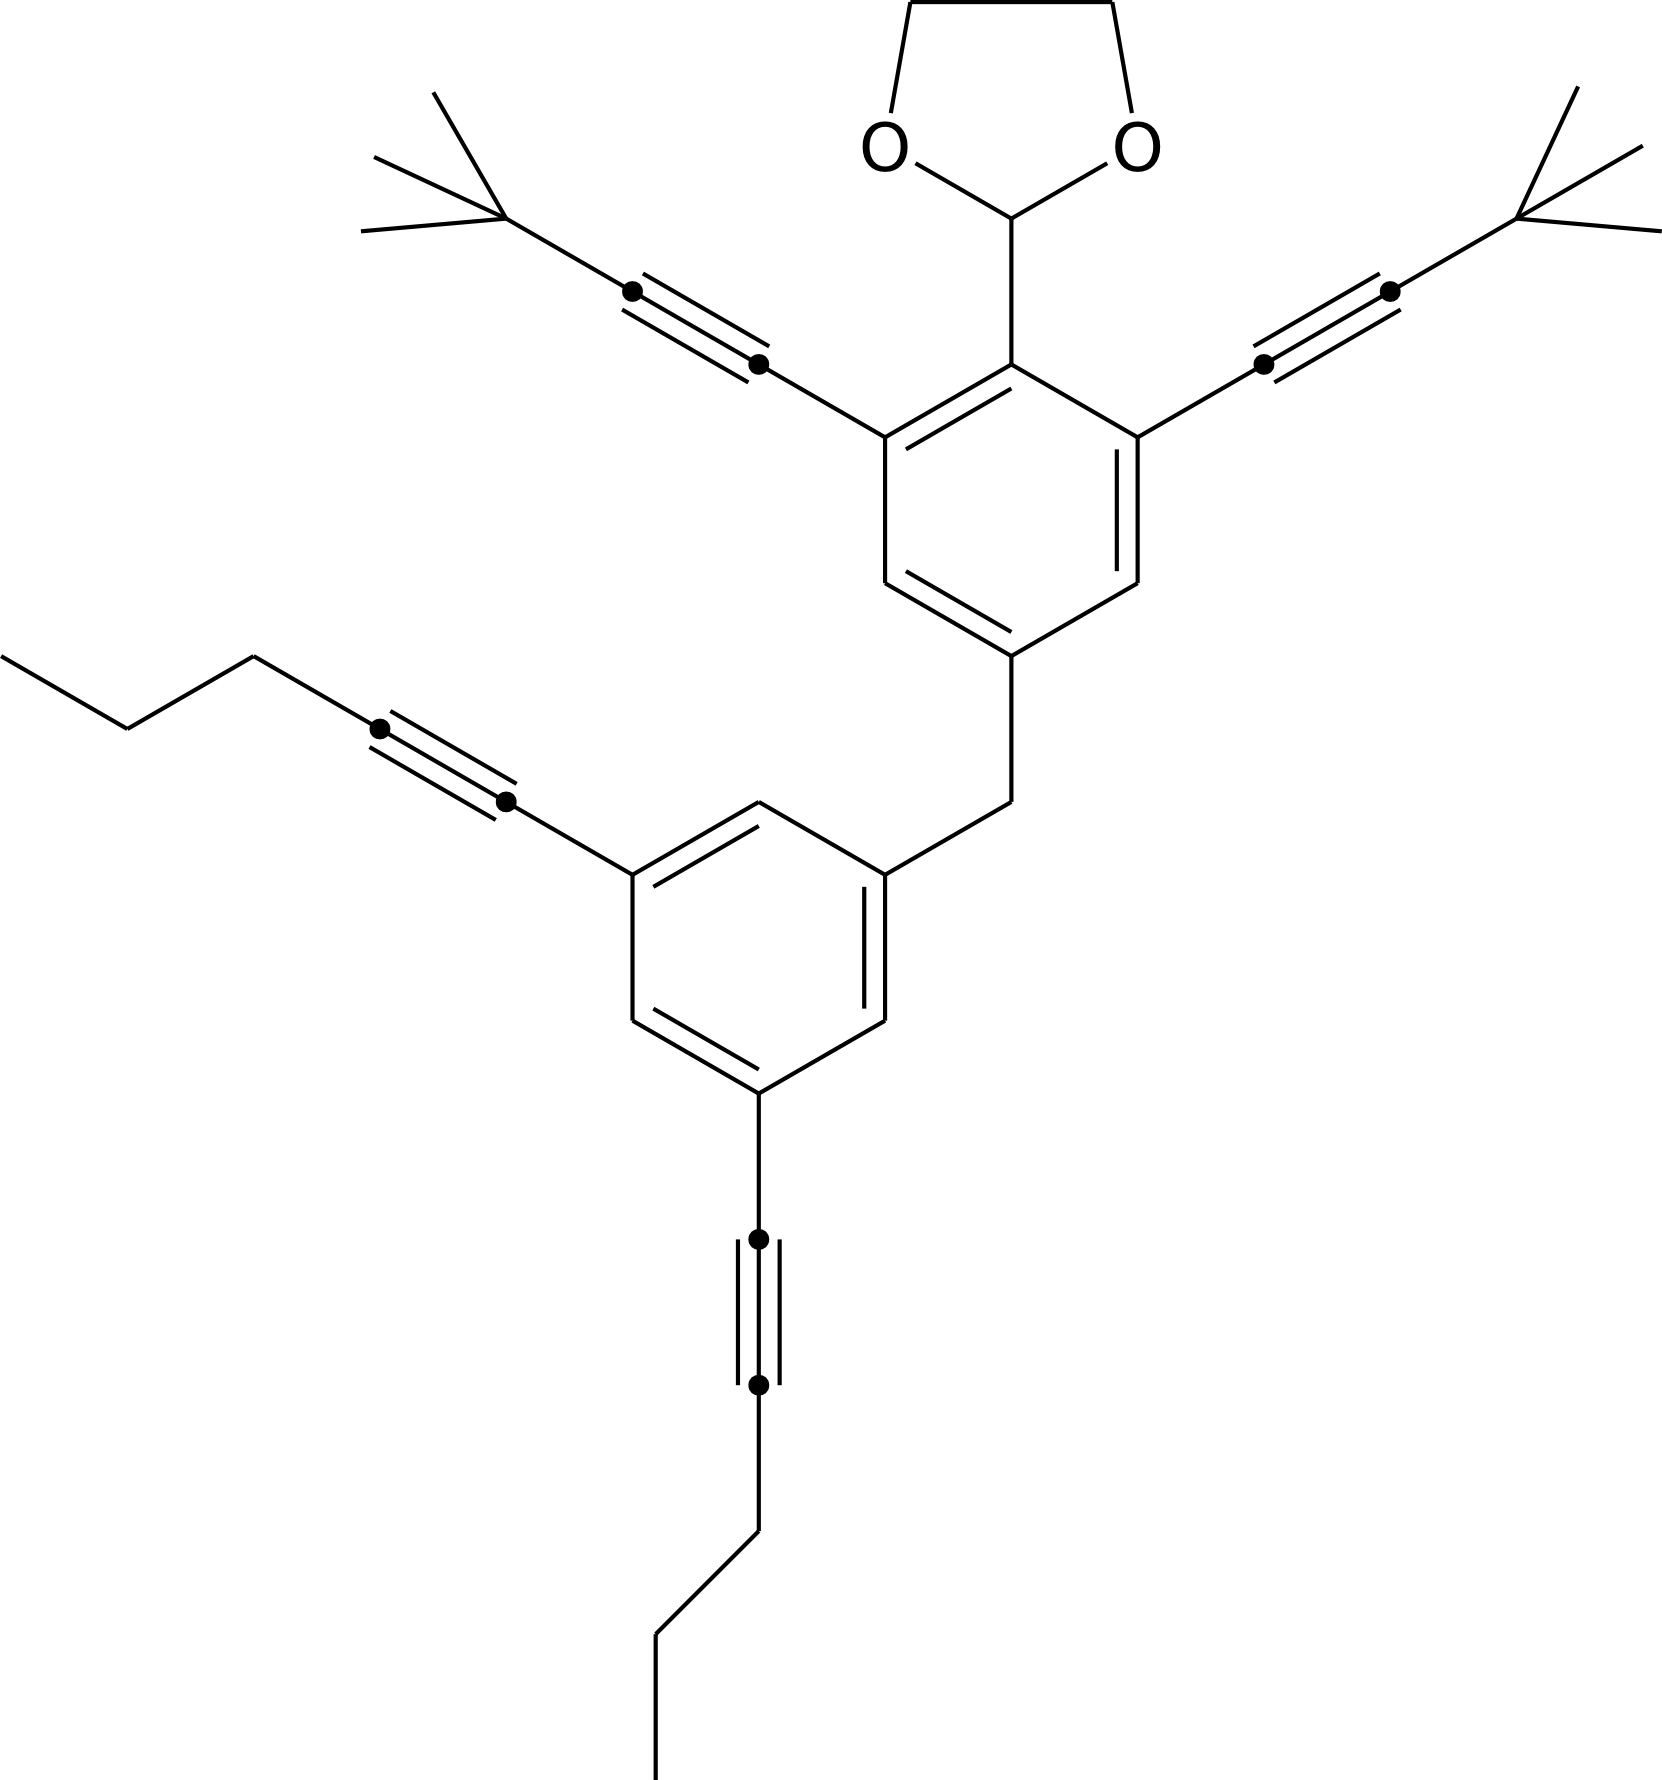
\includegraphics[width=5cm]{20_2016_Litvenenka1.png}
  \caption{Пример органической молекулы, нарисованный в GChemPaint (перерисовано автором по формуле, приведенной в работе ~\cite{Litvenenka1}).}
  \label{Litvenenka1}
\end{figure}

Исторически подобный способ изображения молекул (несколько отличающийся по используемым обозначениям) появился в середине XIX века ~\cite{Litvenenka2}. Для нужд современной органической химии были добавлены условные обозначения и стандартные проекции, необходимые для указания конфигурации оптических изомеров (рис. ~\ref{Litvenenka2}) "--- таким образом, этот способ изображения молекул является чем-то средним между 2D и 3D.

\begin{figure}[h!]
  \centering
  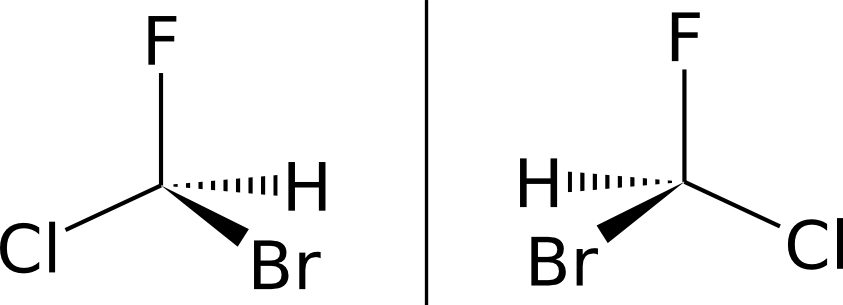
\includegraphics[width=5cm]{20_2016_Litvenenka2.png}
  \caption{Два оптических изомера бромфторхлорметана, отличающиющиеся только ориентацией заместителей. Связь, обозначенная сплошным треугольником, обозначает атом, находящийся перед плоскостью рисунка, штрихованым "--- за плоскостью рисунка.}
  \label{Litvenenka2}
\end{figure}

Дополнительное использование "--- подготовка запросов для поиска по базам данных (по фрагменту структуры), а также для предсказания ЯМР-спектров.

Свободное ПО для 2D-визуализации (GChemPaint, BKChem) существует, однако имеет очень бедный функционал и проигрывает в сравнении с проприетарными аналогами (ACD/ChemSketch, ISIS/Draw). Шаблоны для LaTeX еще беднее по возможностям и используются крайне редко.

\subsubsection*{3D визуализаторы}

Изображают координаты атомов в трехмерном пространстве, а также, опционально, связность.

Молекула может быть представлена как набор атомных ядер, вокруг которых расположены электроны (которые могут быть представлены в виде некоторого распределения электронной плотности, подчиняющегося уравнениям квантовой химии). Скорость движения ядер считается существенно более низкой, чем скорость движения электронов, что позволяет эти движения рассматривать независимо друг от друга (принцип Борна-Оппенгеймера). Таким образом, координаты атомов представляют собой координаты их центров (ядер), причем в зависимости от целей исследования может рассматриваться как некоторые статические координаты, так и анимация движения ядер. Что касается электронной плотности вокруг ядер, то ее полное представление как функции от пространственных координат очень сложно для наглядного построения и малоинформативно, потому применяются (рис. ~\ref{Litvenenka3}), в зависимости от задач, упрощенные модели (следует отметить, что понятие связи при таком подходе также является в значительной степени модельным):

\begin{itemize}
  \item Каркас;
  \item Стержни;
  \item Шары и стержни;
  \item Сферы ван дер Ваальса.
\end{itemize}

\begin{figure}[h!]
  \centering
  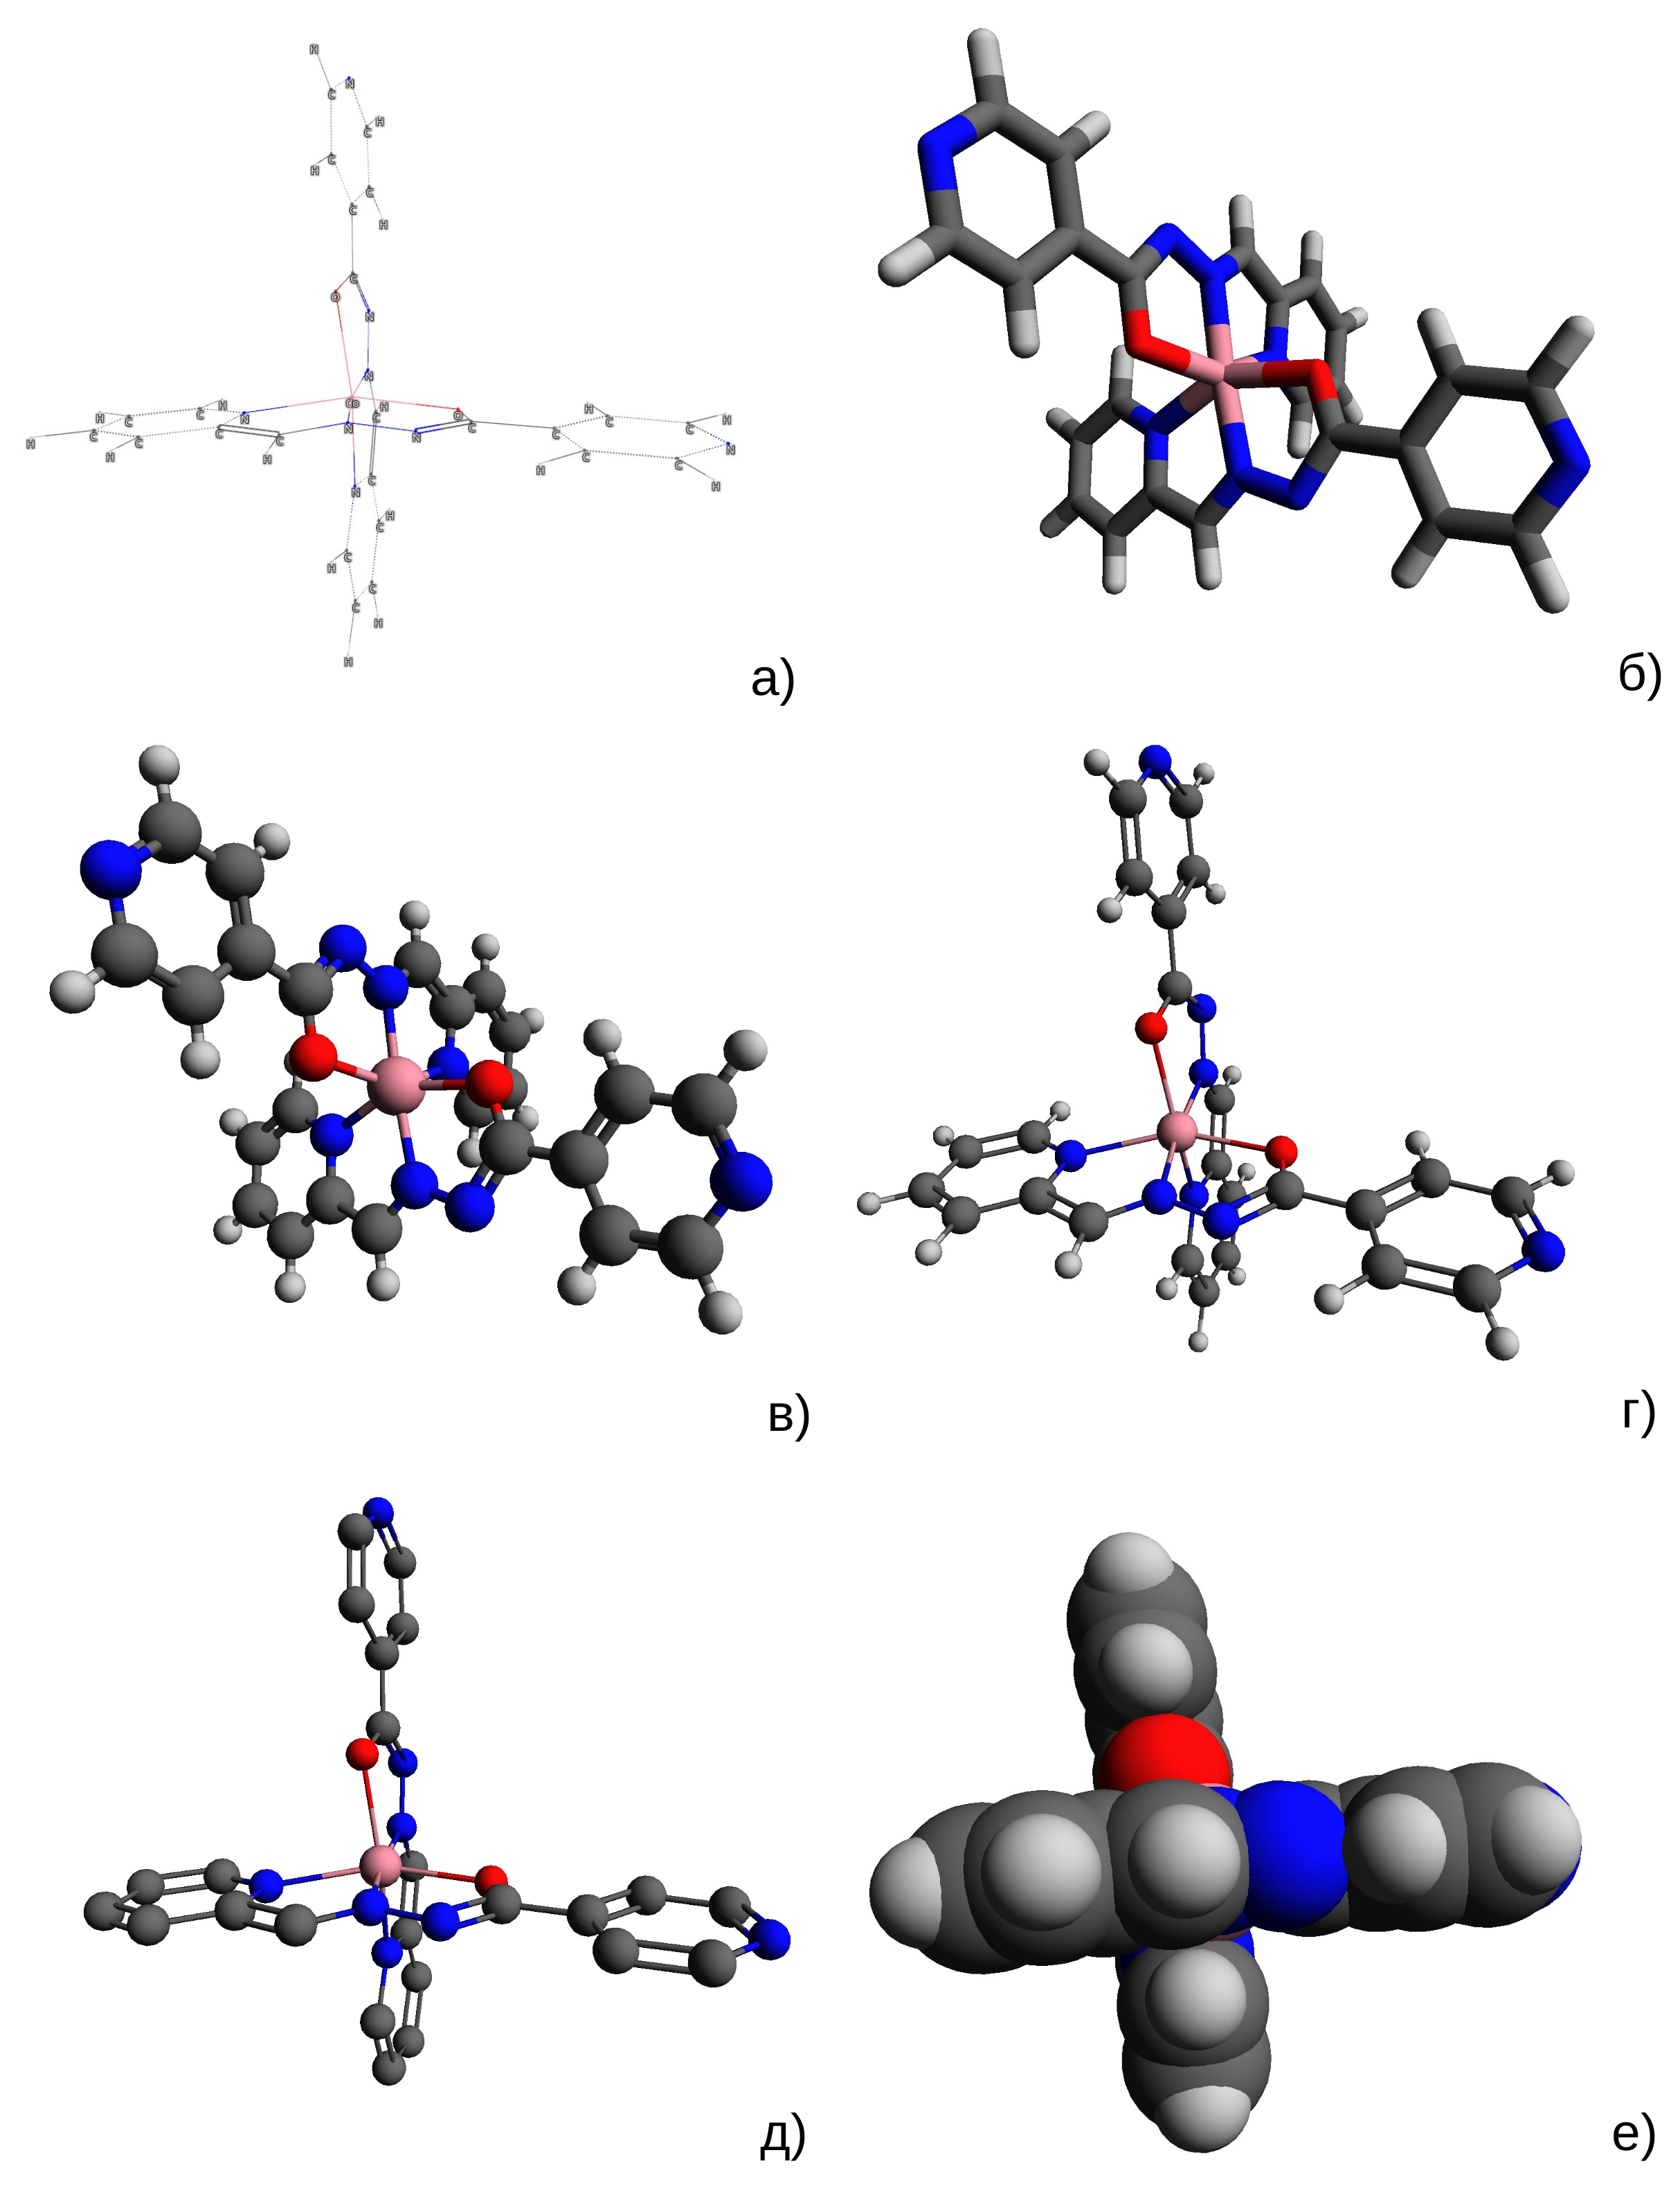
\includegraphics[width=8cm]{20_2016_Litvenenka3.png}
  \caption{Разные способы отображения 3D геометрии молекулы (оптимизированная путем квантовохимического моделирования геометрия комплексного соединения кобальта(II) с основанием Шиффа из 2-пиридилкарбальдегида и гидразида 4-пиридилкарбоновой кислоты, моделирование описано нами в работе ~\cite{Litvenenka2}): а) каркас; б) стержни; в) шары и стержни; г) шары и стержни с уменьшенными радиусами; д) шары и стержни с уменьшенными радиусами без атомов водорода; е) сферы ван дер Ваальса. Построено с использованием программы Avogadro.}
  \label{Litvenenka3}
\end{figure} 

Размеры изображений атомов и связей во всех моделях, кроме размеров сфер ван дер Ваальса, являются условными величинами, и их выбор определяется исключительно удобством представления "--- чем больше размеры, тем легче восприятие отдельных атомов, но тем больше атомы заслоняют друг друга. Для общего анализа геометрии сложной молекулы, состоящей из сотен атомов, больше подойдет изображение в виде каркаса, для подробного анализа более простых молекул "--- шаростержневая модель. Особое место занимает отображение атомов в виде сфер с радиусом, равным ван-дер-ваальсовским радиусам этих атомов, которое позволяет оценить пространство, доступное для других молекул.

В отличие от 2D-рисунков, использование меток и подписей в 3D-изображениях молекулярных структур ограничено, потому более интенсивно используются цветовые схемы (например, раскрашивание атомов разных элементов в разные цвета). Это ведет к получению более эффектных изображений, но усложняет подготовку рисунков для черно-белой печати.

Примеры свободных программ: Avogadro, Gabedit, PyMOL. В целом, наиболее известные и продвинутые 3D визуализаторы относятся к свободному ПО.

3D-визуализаторы, как правило, имеют инструменты для вращения, приближения-удаления, перемещения изображаемой молекулы, а также для измерения расстояний между атомами, углов между тройками атомов, а также диэдральных углов между плоскостями, задаваемыми четырьмя атомами.

В ситуациях, когда координаты атомов в некоторой молекуле из эксперимента неизвестны, и необходимо получить приближенное строение молекулы, для которой известно только химическое строение (связность атомов), важным функционалом 3D-визуализаторов является возможность <<рисования>> молекул и первичной оптимизации их геометрии (последняя, как правило, заключается поиске геометрии, имеющей минимальную энергию, методом молекулярной механики, в ряде случаев с применениями ограничений на изменения координат). Примером программы, реализующей такую возможность, является Avogadro, основанная на библиотеке OpenBabel (которая, среди других вариантов, реализует силовое поле UFF ~\cite{Litvenenka4}, параметризованное для всех элементов от водорода до лоуренсия, что позволяет <<рисование>> как органических, так и неорганических, в том числе металлокомплексных, молекул).

3D-визуализаторы используются также как средство для анализа результатов квантовохимического моделирования, в том числе построения изображений молекулярных орбиталей (рис. ~\ref{Litvenenka4}), форм нормальных колебаний (в виде векторов или в виде анимации), траекторий молекулярной динамики и т.д.

\begin{figure}[h!]
  \centering
  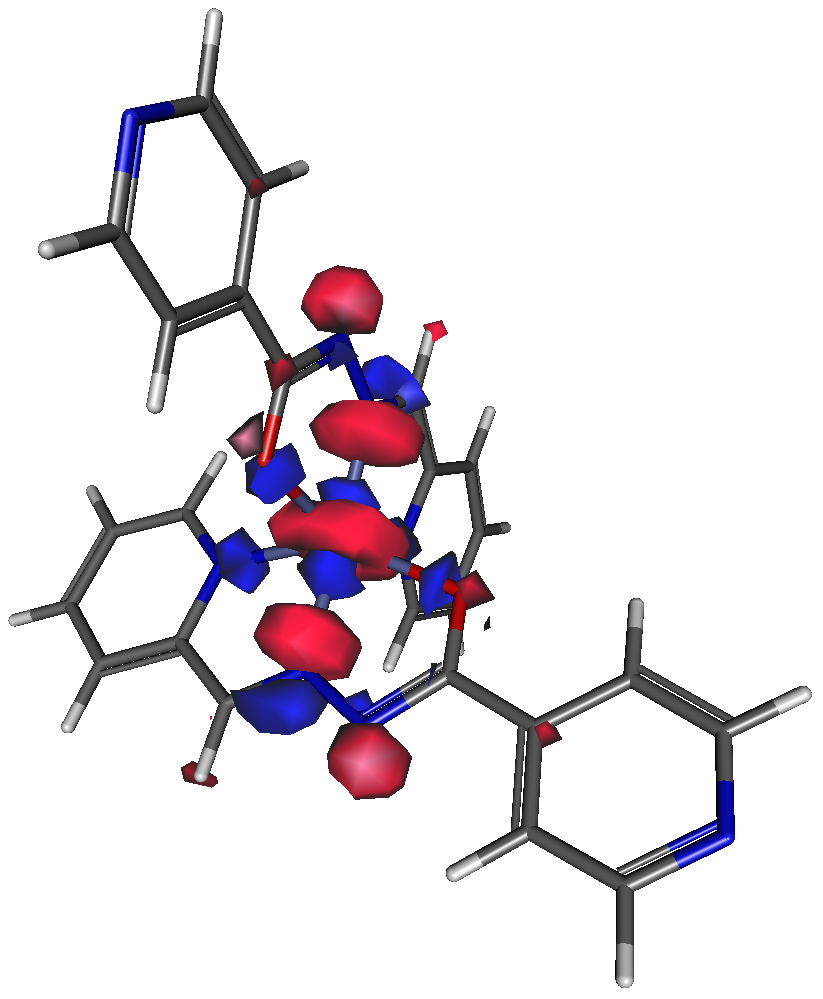
\includegraphics[width=5cm]{20_2016_Litvenenka4.png}
  \caption{75\% изоповерхность высшей занятой молекулярной орбитали (α) комплексного соединения кобальта(II) с основанием Шиффа из 2-пиридилкарбальдегида и гидразида 4-пиридилкарбоновой кислоты (моделирование описано нами в работе ~\cite{Litvenenka3}), сгенерированная с помощью программы Gabedit.}
  \label{Litvenenka4}
\end{figure} 


Полученные изображения молекулярных структур сохраняются в специальных форматах (как правило, содержащих в том или ином виде координаты атомов и описание связей) и могут быть экспортированы в растровые или векторные изображения (в отличие от 2D-редакторов, возможности по добавлению текста или элементов схем в 3D редакторах намного беднее, однако, это можно сделать с помощью графических редакторов). Кроме того, ряд программ имеет возможность экспортировать сценарий для создания POV-Ray сцены (с ограниченными настройками, рис. ~\ref{Litvenenka5}).

\begin{figure}[h!]
  \centering
  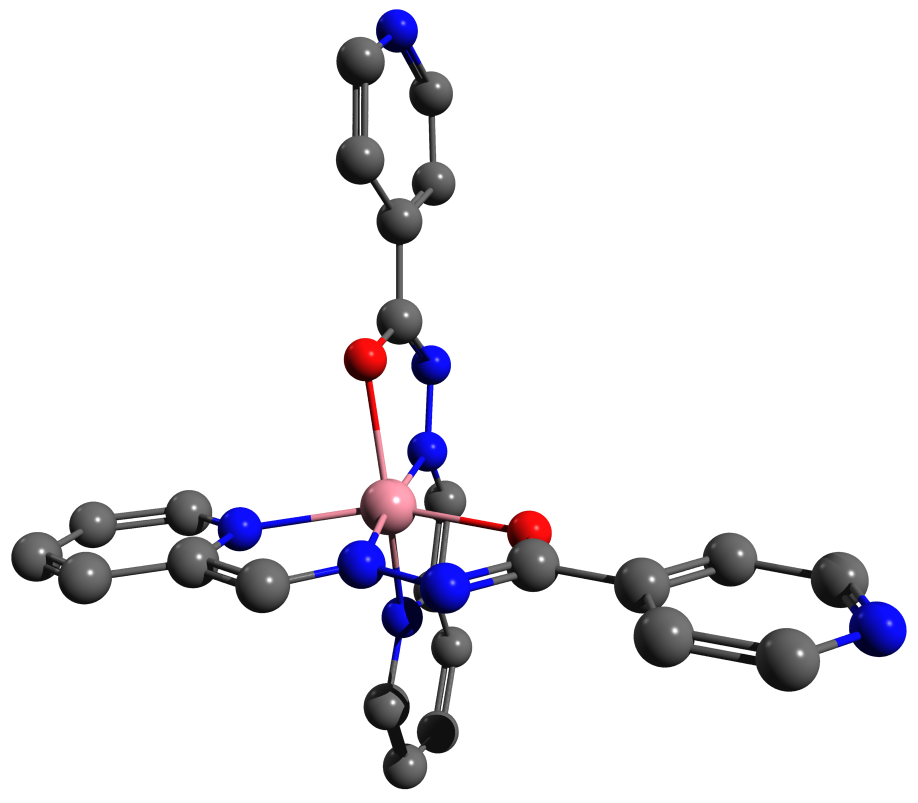
\includegraphics[width=5cm]{20_2016_Litvenenka5.png}
  \caption{3D геометрия молекулы (оптимизированная путем квантовохимического моделирования геометрия комплексного соединения кобальта(II) с основанием Шиффа из 2-пиридилкарбальдегида и гидразида 4-пиридилкарбоновой кислоты, моделирование описано нами в работе ~\cite{Litvenenka3}) в виде шаростержневой модели с уменьшенными радиусами без атомов водорода, сгенерированная с помощью POV-Ray, исходный файл для рендеринга создан программой Avogadro.}
  \label{Litvenenka5}
\end{figure} 
  
Существуют плагины, позволяющие работу с молекулами в \linebreak Blender, однако их функционал, равно как и размер импортируемых молекул, ограничены.

\subsubsection*{Визуализаторы кристаллических структур.}

Во многом похожи на 3D-визуализаторы, но отличаются полноценной возможностью работать с кристаллическими структурами "--- бесконечными периодическими системами (рис. ~\ref{Litvenenka6}). Соответственно, этот класс программ имеет возможность размножать элементы кристаллической решетки необходимое число раз операциями трансляции, ограничивать отображение отдельными цепочками или слоями с учетом трансляций, наращивать отображаемую структуру с учетом трансляций, ориентировать структуру вдоль осей элементарной ячейки и т.д. Дополнительными востребованными возможностями является анализ пористой структуры "--- объем (процент) пустот в кристалле, диаметр и форма пор, в том числе (в случае пор сложного строения) диаметр и форма сужений и расширений пор. Некоторые визуализаторы кристаллических структур (или сопряженные с ними программы) умеют также получать структуры путем обработки данных рентгеноструктурного анализа.

\begin{figure}[h!]
  \centering
  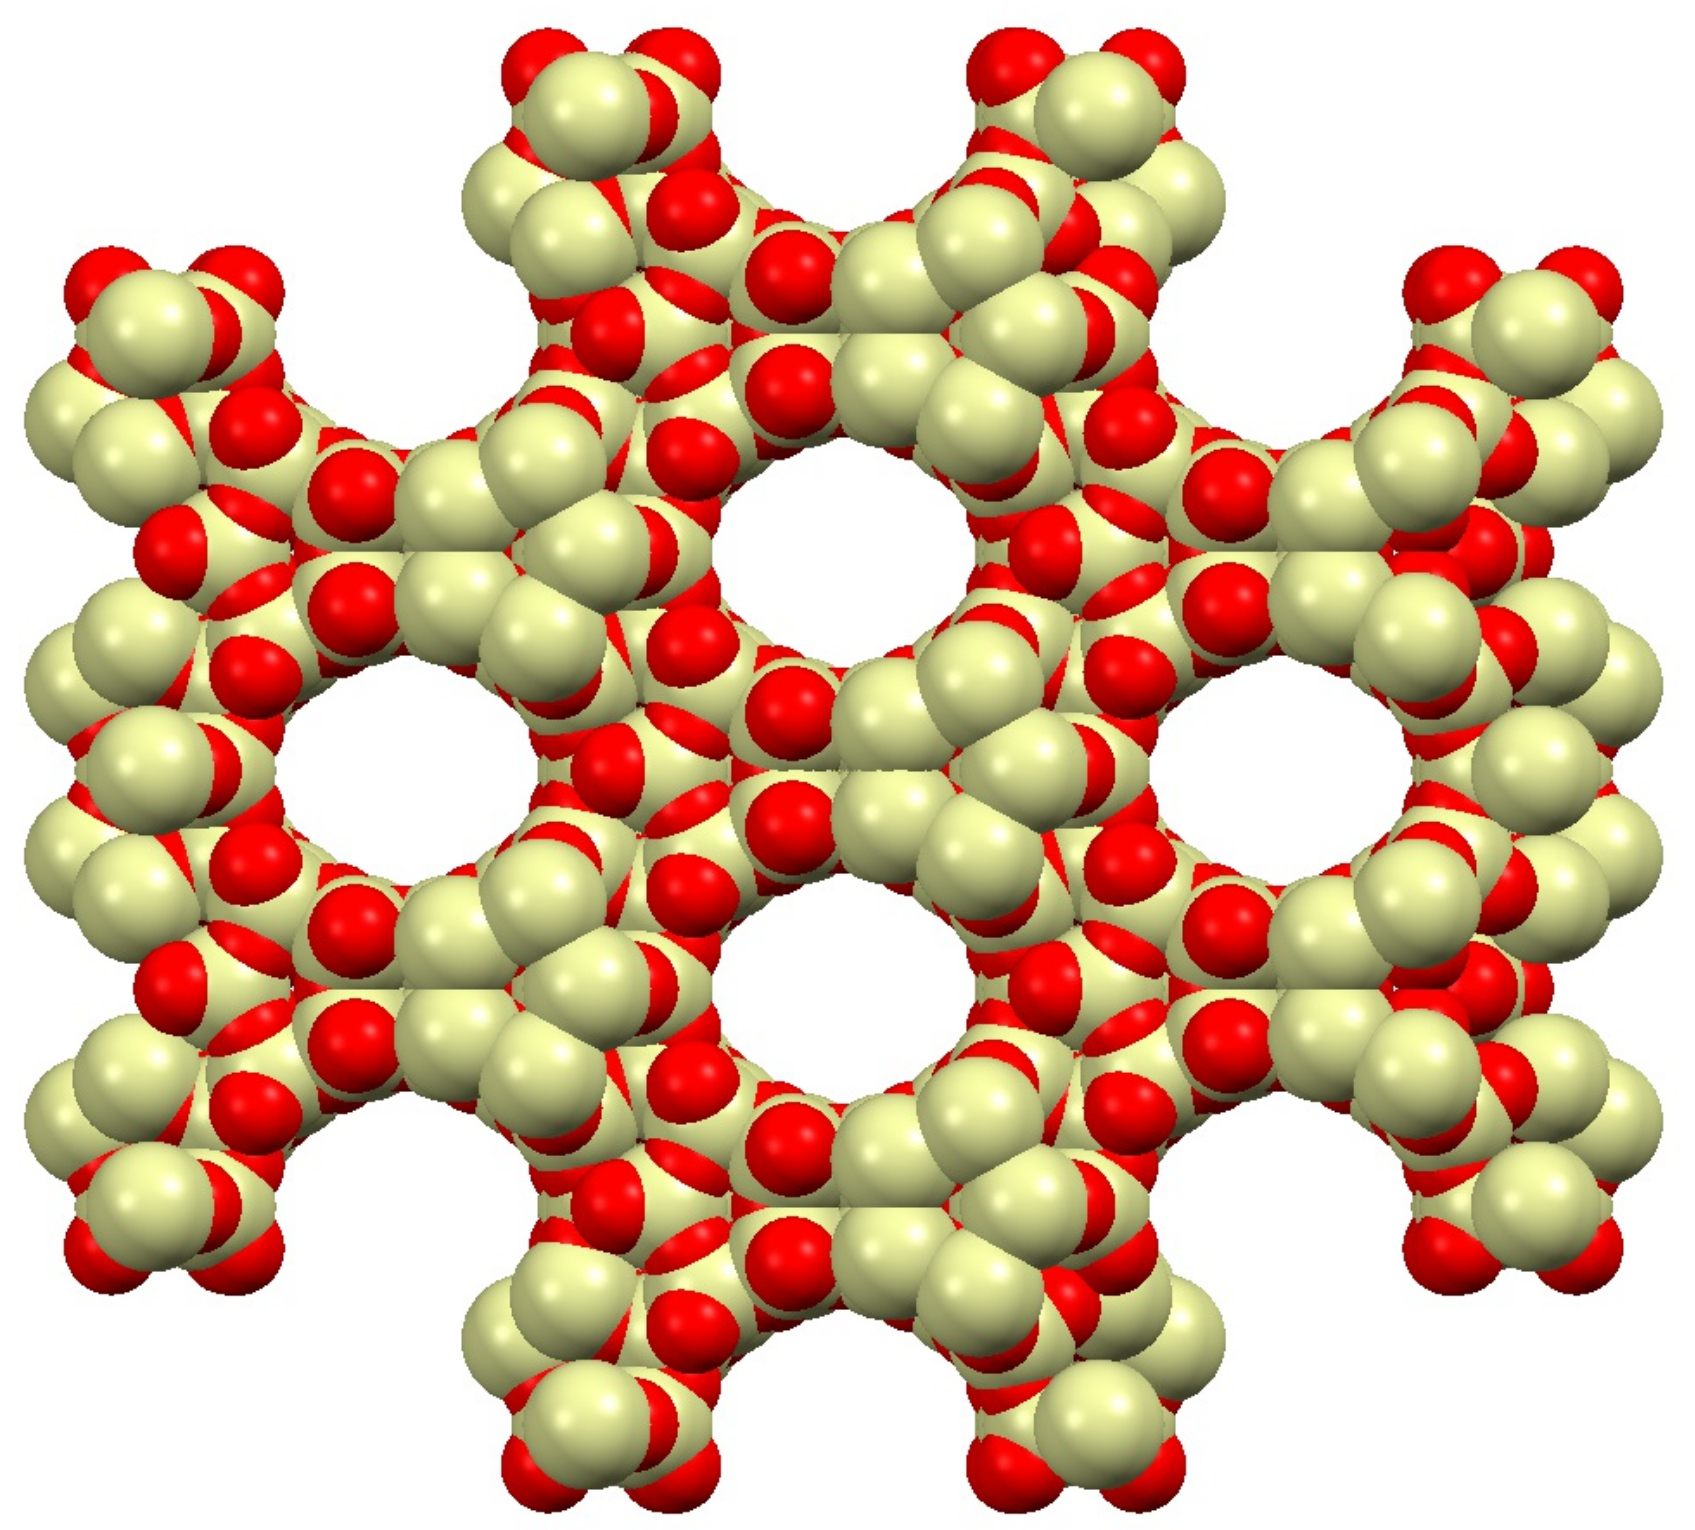
\includegraphics[width=5cm]{20_2016_Litvenenka6.png}
  \caption{Кристаллическая структура цеолита UTL, построенная в програме Mercury (proprietary freeware), модель — сферы ван дер Ваальса. На рисунке видны поры кристаллической структуры UTL.}
  \label{Litvenenka6}
\end{figure} 
К сожалению, в свободном ПО возможности работы с кристаллическими структурами крайне ограничены.

\subsubsection*{Текущие проблемы и задачи.}

\begin{itemize}
  \item Потребность в новых возможностях манипуляции кристаллическими структурами, в частности, подготовка входных данных и анализ результатов для квантовохимических расчетов с периодическими краевыми условиями (генерация суперячеек, преобразование в специфические форматы файлов, добавление гостевых молекул и т.д.);
  \item Продвинутый анализ микропористой (с диаметром пор до 2 нм) структуры: характеризация размеров и формы пор с учетом того, что размер поры сравним с размерами атомов (т.е. форма поры в значительной степени определяется расположением отдельных атомов);
  \item Поиск ответа на вопрос о возможности вхождения гостевой молекулы в микропору "--- геомерические критерии для сложных по форме пор и молекул, энергетические критерии (энергия активации диффузии молекулы в поре).
\end{itemize}

Для решения части этих задач нужен поиск или написание программного обеспечения, способного выполнять соответствующие \linebreak действия, тогда как для последней задачи необходима разработка новых теоретических подходов. Некоторые работы на уровне \emph{proof of concept} ведутся нами: так, доступность пор координационного полимера HKUST-1 (бензолтрикарбоксилата меди), катализирующего сочетание салицилового альдегида с нитрометаном с образованием \emph{транс}-нитровинилфенола, для реагентов и продукта реакции была показана нами путем определения величины энергии активации диффузии молекул в поре HKUST-1 методом молекулярной механики ~\cite{Litvenenka5}.

\subsubsection*{Выводы.}

Таким образом, программное обеспечение для визуализации химического строения вещества является важным инструментом в работе химика, применяемым для ряда связанных между собой задач: анализа строения вещества, подготовки и интерпретации результатов компьютерного моделирования химических веществ и процессов, а также подготовки материалов для публикаций. Свободное ПО такого типа развито недостаточно (за исключением 3D-визуализаторов молекулярных структур). Кроме того, в современной химии существуют задачи по анализу строения химических веществ, не решаемые или плохо решаемые с помощью существующих программ (в особенности свободных). Дальнейшее развитие визуализаторов химического строения вещества требует совместной работы специалистов в области химии и программирования и представляет собой важную задачу для развития современной химической науки.

\begin{thebibliography}{99}

\bibitem{Litvenenka1} S. H. Chanteau, J. M. Tour, <<Synthesis of Anthropomorphic Molecules:  The NanoPutians>>, \emph{J. Org. Chem.}, \textbf{2003}, 68(23):8750–8766.
\bibitem{Litvenenka2} A. Crum Brown, <<On the Theory of Isomeric Compounds>>, \emph{Transactions of the Royal Society of Edinburgh}, \textbf{1864}, 23:707–719.
\bibitem{Litvenenka3} A. S. Lytvynenko,   S. V. Kolotilov, M. A. Kiskin, I. L. Eremenko, V. M. Novotortsev, <<Modeling of catalytically active metal complex species and intermediates in reactions of organic halides electroreduction>>, \emph{Phys. Chem. Chem. Phys}, \textbf{2015}, 17:5594–5605
\bibitem{Litvenenka4} A. K. Rappe, C. J. Casewit, K. S. Colwell, W. A. Goddard III, W. M. Skiff, <<UFF, a full periodic table force field for molecular mechanics and molecular dynamics simulations>>, \emph{J. Am. Chem. Soc.}, \textbf{1992}, 114(25):10024–10035.
\bibitem{Litvenenka5} S. A. Sotnik, K. S. Gavrilenko, A. S. Lytvynenko, S. V. Kolotilov, <<Catalytic activity of copper(II) benzenetricarboxylate (HKUST-1) in reactions of aromatic aldehydes condensation with nitromethane: Kinetic and diffusion study>>, \emph{Inorg. Chim. Acta}, \textbf{2015}, 426:119–125.
\end{thebibliography}
\end{document}

\documentclass[10pt, a5paper]{article}
\usepackage{pdfpages}
\usepackage{parallel}
\usepackage[T2A]{fontenc}
\usepackage{ucs}
\usepackage[utf8x]{inputenc}
\usepackage[polish,english,russian]{babel}
\usepackage{hyperref}
\usepackage{rotating}
\usepackage[inner=2cm,top=1.8cm,outer=2cm,bottom=2.3cm,nohead]{geometry}
\usepackage{listings}
\usepackage{graphicx}
\usepackage{wrapfig}
\usepackage{longtable}
\usepackage{indentfirst}
\usepackage{array}
\newcolumntype{P}[1]{>{\raggedright\arraybackslash}p{#1}}
\frenchspacing
\usepackage{fixltx2e} %text sub- and superscripts
\usepackage{icomma} % коскі ў матэматычным рэжыме
\PreloadUnicodePage{4}

\newcommand{\longpage}{\enlargethispage{\baselineskip}}
\newcommand{\shortpage}{\enlargethispage{-\baselineskip}}

\def\switchlang#1{\expandafter\csname switchlang#1\endcsname}
\def\switchlangbe{
\let\saverefname=\refname%
\def\refname{Літаратура}%
\def\figurename{Іл.}%
}
\def\switchlangen{
\let\saverefname=\refname%
\def\refname{References}%
\def\figurename{Fig.}%
}
\def\switchlangru{
\let\saverefname=\refname%
\let\savefigurename=\figurename%
\def\refname{Литература}%
\def\figurename{Рис.}%
}

\hyphenation{admi-ni-stra-tive}
\hyphenation{ex-pe-ri-ence}
\hyphenation{fle-xi-bi-li-ty}
\hyphenation{Py-thon}
\hyphenation{ma-the-ma-ti-cal}
\hyphenation{re-ported}
\hyphenation{imp-le-menta-tions}
\hyphenation{pro-vides}
\hyphenation{en-gi-neering}
\hyphenation{com-pa-ti-bi-li-ty}
\hyphenation{im-pos-sible}
\hyphenation{desk-top}
\hyphenation{elec-tro-nic}
\hyphenation{com-pa-ny}
\hyphenation{de-ve-lop-ment}
\hyphenation{de-ve-loping}
\hyphenation{de-ve-lop}
\hyphenation{da-ta-ba-se}
\hyphenation{plat-forms}
\hyphenation{or-ga-ni-za-tion}
\hyphenation{pro-gramming}
\hyphenation{in-stru-ments}
\hyphenation{Li-nux}
\hyphenation{sour-ce}
\hyphenation{en-vi-ron-ment}
\hyphenation{Te-le-pathy}
\hyphenation{Li-nux-ov-ka}
\hyphenation{Open-BSD}
\hyphenation{Free-BSD}
\hyphenation{men-ti-on-ed}
\hyphenation{app-li-ca-tion}

\def\progref!#1!{\texttt{#1}}
\renewcommand{\arraystretch}{2} %Іначай формулы ў матрыцы зліпаюцца з лініямі
\usepackage{array}

\def\interview #1 (#2), #3, #4, #5\par{

\section[#1, #3, #4]{#1 -- #3, #4}
\def\qname{LVEE}
\def\aname{#1}
\def\q ##1\par{{\noindent \bf \qname: ##1 }\par}
\def\a{{\noindent \bf \aname: } \def\qname{L}\def\aname{#2}}
}

\def\interview* #1 (#2), #3, #4, #5\par{

\section*{#1\\{\small\rm #3, #4. #5}}

\def\qname{LVEE}
\def\aname{#1}
\def\q ##1\par{{\noindent \bf \qname: ##1 }\par}
\def\a{{\noindent \bf \aname: } \def\qname{L}\def\aname{#2}}
}

\begin{document}
\title{Enterprise Storage OS (ESOS)\footnote{\url{alex_kls@mail.ru}, \url{http://lvee.org/ru/abstracts/219}}}
\author{Александр Клыга, Минск, Беларусь}
\maketitle
\begin{abstract}
The Enterprise Storage OS (ESOS) is open-source software to build the Data Storages System within the SAN model. The ESOS is a compact Linux distribution and it is distributed under a GPL license. In my presentation the main components of the ESOS are considered including a loading method and the Data Storages System architecture.
\end{abstract}
%\textbf{Enterprise Storage OS (ESOS).}

Создание и обслуживание сетей хранения данных (Storage Area Network или сокращенно SAN) одна из интересных технических задач для технических специалистов обслуживающих системы хранения данных в различных компаниях. Прежде всего это обусловлено самой моделью SAN, и техническими требованиями предъявляемыми к системе хранения данных в целом, особенно с учетом широкого использования средств визуализации и необходимостью хранить большие объемы данных.

Очень часто техническим специалистам, сопровождающим крупные системы хранения данных, приходится решать трудные задачи, связанные с расширением объема доступного дискового пространства, надежностью хранения информации и интеграции с другими СХД, в частности с распределенными файловыми системами. Именно поэтому поиск оптимального решения подобных задач является критически важным, а оптимальный вариант должен обеспечивать должный уровень надежности, гибкости и возможности гибкого расширения без сложных структурных реорганизаций.

Поэтому вполне логично, что поиск решений для оптимизации и расширения существующей корпоративной архитектуры сети хранения данных начинается с решений на рынке свободного программного обеспечения (обзор некоторых из них был представлен мною в рамках доклада «Обзор решений на рынке открытого ПО для создания СХД» на зимней сессии LVEE в феврале этого года~\cite{Kliga1}). По совету коллег несколько лет назад я обратил внимание на один очень интересный проект  Enterprise Storage OS (ESOS)~\cite{Kliga2}.

В ESOS основное внимание у меня привлекло возможность создания дисковых хранилищ для систем хранения данных модели SAN и возможности интеграции существующей SAN в объектное хранилище данных Ceph. 
С физической точки зрения отдельное дисковое хранилище в SAN представляет собой законченное техническое решение состоящее отдельных дисковых полок (с установленных в них дисками)  подключенных к контроллеру управления, а для подключения к сетевой инфраструктуре SAN  на нем устанавливаются HBA (host bus adapter) адаптеры. Управление оборудованием осуществляется через консоль или по локальной сети \linebreak через специальное приложение установленное на компьютере или web – приложение.

Но прежде чем приступить к описанию всех достоинств использования ESOS в SAN, необходимо кратко рассмотреть ее  физическую и программную модели.

Физическая модель SAN состоит из трех основных компонентов: серверной фермы, сетевой инфраструктуры и дискового массива. В состав серверной фермы SAN входят сервера SAN не имеющих собственной подсистемы дисковой памяти и подключаются к сетевой инфраструктуре хранилища через специальный адаптеры HBA (host bus adapter). В состав сетевой архитектуры SAN входит активное сетевое оборудование (концентраторы, коммутаторы, мосты, маршрутизаторы)   и пассивное оборудование (кабели, коннекторы). В состав дискового массива входят  специализированные дисковые стойки (устройства состоящие из десятков дисков управляемые контроллером или сервером) подключаемые к сетевой инфраструктуру через адаптеры HBA.

Программная модель взаимодействия основных компонентов \linebreak SAN между собой базируется на клиент-серверной модели семейства протоколов Small Computer System Interface (SCSI). Согласно ее клиентские приложения устанавливаются на сервера серверной фермы SAN, сервер выступает в роли инициатора (Initiator) сессии взаимодействия с целевым устройством (Target) в дисковой подсистемой хранилища через сетевую инфраструктуру SAN. Target  обрабатывает команды адресуемые ему от Initiator и формирует ответ.

При казалось бы видимой простоте программной модели следует отметить важные моменты:

\begin{itemize}
  \item взаимодействия между Initiator и Target осуществляется блоками заданной длины (т. е. все устройства представляются в виде сетевых блочных устройств);
  \item Target это логическое устройство которому присвоен уникальный номер, и с одним Target могут взаимодействовать несколько Initiator;
  \item Initiator не взаимодействует напрямую с дисками в хранилище данных, а использует одно или несколько логических устройств с уникальным номером — LUN (logical unit number);
  \item LUN абстрагирован от физической архитектуры дискового хранилища и представляет собой виртуальный диск созданный посредством специального ПО.
\end{itemize}

Таким образом, становится очевидно, первое, что сервер SAN подключенный с сети хранения данных напрямую не управляет физическими дисками подключенными к нему, все манипуляции с ними осуществляет через LUN (один или несколько) на Target. Второе Target может быть как отдельное физическое хранилище имеющий свой уникальный физический номер, так и  может выступать как программный интерфейс к распределенной файловой системе через блочный интерфейс доступа. При этом логический номер Target присваиваться в программном обеспечении  контроллера  (сервера) управляющего дисковым хранилищем (Data Storage) или сервера на котором установлено программное обеспечение интерфейса блочного доступа к распределенной файловой системе или другому хранилищу данных.

При этом важно отметить, что сервера серверной фермы SAN не имеют собственной подсистемы дисковой памяти и с точки зрения физической архитектуры, LUN выделенный на Target для сервера,  представляет собой обычный физический диск на который будет установлена операционная система для развертывания клиентского ПО. Следовательно программное обеспечение с помощью которого создается LUN должно поддерживать эмуляцию большинства типов файловых систем в том числе гипервизоров систем виртуализации, например, VMware.

К моему удивлению все это было объединено в проекте ESOS. В его основе был положен проект SCST (Generic SCSI Target \linebreak Subsystem for Linux)~\cite{Kliga3}, дополненный всеми необходимыми инструментами управления дисками (включая поддержку RAID-массивов), пакетами драйверов поддержки инфраструктуры SAN (оборудования производства QLogic, Emulex и других вендоров), мониторинга работы сервера и компонентами для поддержки пулов хранения в формате VMFS VMware ESX/ESXi, томов Windows NTFS и дисков Linux. Что дает возможность создавать хранилища данных (Data Storage) для SAN на базе серверов модели DAS~\cite{Kliga1}.
Также в состав компонентов ESOS входят модули поддержки распределенной файловой системы Ceph (в частности используется Ceph RBD в качестве оконечных устройств хранения данных) и поддержки кластеризации (Pacemaker\&Corosync и DRBD).

Исходные коды ESOS находятся на GitHub ~\cite{Kliga4} и компилируется виде Linux-дистрибутива с очень компактным кодом и распространяется под лицензией GPL. Ключевой особенностью ESOS является его полное резидентное расположении в памяти, при этом загрузка осуществляется с USB-накопителя и не требует отдельного диска для установки дистрибутива. При этом реализованы механизмы восстановления работоспособности системы в случае сбоев.

\begin{thebibliography}{99}

\bibitem{Kliga1} А. Клыга. Обзор решений на рынке открытого ПО для создания СХД // Материалы конференции LVEE Winter 2016, Минск, 12-14 ферваля 2016 г. \url{https://lvee.org/ru/abstracts/181}
\bibitem{Kliga2} ESOS: ESOS -- Enterprise Storage OS // ESOS \url{http://www.esos-project.com}
\bibitem{Kliga3} SCST GENERIC SCSI TARGET SUBSYSTEM FOR LINUX // SCST Project \url{http://scst.sourceforge.net/}
\bibitem{Kliga4} The project ESOS on GitHub // ESOS on GitHub \url{https://github.com/parodyne/esos}
\end{thebibliography}
\end{document}

\documentclass[10pt, a5paper]{article}
\usepackage{pdfpages}
\usepackage{parallel}
\usepackage[T2A]{fontenc}
\usepackage{ucs}
\usepackage[utf8x]{inputenc}
\usepackage[polish,english,russian]{babel}
\usepackage{hyperref}
\usepackage{rotating}
\usepackage[inner=2cm,top=1.8cm,outer=2cm,bottom=2.3cm,nohead]{geometry}
\usepackage{listings}
\usepackage{graphicx}
\usepackage{wrapfig}
\usepackage{longtable}
\usepackage{indentfirst}
\usepackage{array}
\newcolumntype{P}[1]{>{\raggedright\arraybackslash}p{#1}}
\frenchspacing
\usepackage{fixltx2e} %text sub- and superscripts
\usepackage{icomma} % коскі ў матэматычным рэжыме
\PreloadUnicodePage{4}

\newcommand{\longpage}{\enlargethispage{\baselineskip}}
\newcommand{\shortpage}{\enlargethispage{-\baselineskip}}

\def\switchlang#1{\expandafter\csname switchlang#1\endcsname}
\def\switchlangbe{
\let\saverefname=\refname%
\def\refname{Літаратура}%
\def\figurename{Іл.}%
}
\def\switchlangen{
\let\saverefname=\refname%
\def\refname{References}%
\def\figurename{Fig.}%
}
\def\switchlangru{
\let\saverefname=\refname%
\let\savefigurename=\figurename%
\def\refname{Литература}%
\def\figurename{Рис.}%
}

\hyphenation{admi-ni-stra-tive}
\hyphenation{ex-pe-ri-ence}
\hyphenation{fle-xi-bi-li-ty}
\hyphenation{Py-thon}
\hyphenation{ma-the-ma-ti-cal}
\hyphenation{re-ported}
\hyphenation{imp-le-menta-tions}
\hyphenation{pro-vides}
\hyphenation{en-gi-neering}
\hyphenation{com-pa-ti-bi-li-ty}
\hyphenation{im-pos-sible}
\hyphenation{desk-top}
\hyphenation{elec-tro-nic}
\hyphenation{com-pa-ny}
\hyphenation{de-ve-lop-ment}
\hyphenation{de-ve-loping}
\hyphenation{de-ve-lop}
\hyphenation{da-ta-ba-se}
\hyphenation{plat-forms}
\hyphenation{or-ga-ni-za-tion}
\hyphenation{pro-gramming}
\hyphenation{in-stru-ments}
\hyphenation{Li-nux}
\hyphenation{sour-ce}
\hyphenation{en-vi-ron-ment}
\hyphenation{Te-le-pathy}
\hyphenation{Li-nux-ov-ka}
\hyphenation{Open-BSD}
\hyphenation{Free-BSD}
\hyphenation{men-ti-on-ed}
\hyphenation{app-li-ca-tion}

\def\progref!#1!{\texttt{#1}}
\renewcommand{\arraystretch}{2} %Іначай формулы ў матрыцы зліпаюцца з лініямі
\usepackage{array}

\def\interview #1 (#2), #3, #4, #5\par{

\section[#1, #3, #4]{#1 -- #3, #4}
\def\qname{LVEE}
\def\aname{#1}
\def\q ##1\par{{\noindent \bf \qname: ##1 }\par}
\def\a{{\noindent \bf \aname: } \def\qname{L}\def\aname{#2}}
}

\def\interview* #1 (#2), #3, #4, #5\par{

\section*{#1\\{\small\rm #3, #4. #5}}

\def\qname{LVEE}
\def\aname{#1}
\def\q ##1\par{{\noindent \bf \qname: ##1 }\par}
\def\a{{\noindent \bf \aname: } \def\qname{L}\def\aname{#2}}
}

\begin{document}
\title{Миграция виртуальной инфраструктуры на свободное ПО XenServer\footnote{\url{arol90@gmail.com}, \url{http://lvee.org/ru/abstracts/220}}}
\author{Антон Новиков, Минск, Беларусь}
\maketitle
\begin{abstract}
Migrate virtual infrastructure to open source XenServer. Real, complete project.
\end{abstract}
\subsection*{Введение}
Виртуализация плотно вошла в «IT  мир», закрепилась в ЦОДах крупного и среднего бизнеса, зачастую внедрение таких систем сопровождается множеством подсчетов и сравнений. Систем с каждым годом, если не сказать месяцем становится больше, времени на реализацию проектов все меньше.
Данная статья о крупный игроке на рынке который отдал свою разработку в заботливые руки Open Source. Это — XenServer. Именно о нем как о представителе СПО этот доклад.

\subsection*{О системах Виртуализации}
Хороших а главное гибких систем не так уж и много. Как правило выделяются всего пара таких проектов. В качестве ярчайших представителей можно уверенно рассматривать XenServer(СПО) и VmWare ESXi. Да существует огромное количество СПО систем виртуализации, которые бесспорно готовы во многом дать преимущество выше указанным гигантам, но в купе всех качеств в итоге проигрывают.

\subsection*{Почему был выбран именно XenServer}
Помимо очевидного — «цены», простота, гибкость, открытость, функционал, сильное комьюнити.
Это далеко не весь перечень, но хватает и минусов и к сожалению весьма досадных, вещи которые в других системах воспринимаются как должное в XenServer отсутствуют вовсе.
Чего только, стоит вопрос с пробросом USB порта в виртуальную систему.

После выбора системы виртуализации предстоял процесс внедрения,  трудоемкий процесс и самое главное в данном мероприятии -- время простоя бизнеса, и к сожалению в финансовой сфере оно равно нулю. Финансовые вложения тоже ограничены и нельзя просто построить рядом еще один ЦОД и мигрировать всё на него, процесс становится многослойным. Перейдем к нему немного детальнее.

Реальный проект перехода системы вирутализации и инфраструктуры крупной финансовой компании на СПО. Была проведена детальная проработка плана перехода, подготовка оборудования, и многие многие иные вопросы упавшие на плечи нашего IT подразделения, и самое главное все это подразумевало непрерывность бизнеса во время и после интеграции.

Был построен HA кластер на основе Blade серверов HP BL-460c
Каким бы свободным не было ПО а серверное оборудования не получится скачать из репозитариев. Вложения в оборудование зачастую в разы выше вложений в персонал или ПО.
Описываемый проект реализован на серверных шасси HP c7000 с использованием FiberChannel в качестве сети хранения данных и HP 3Par 7200 в качестве системы хранения.

Была произведена миграция с проприетарного программного обеспечения на СПО Xenserver.

\subsection*{По итогам проекта} 
Можно сделать вывод, что система справляется с возложенными на неё функциями, отлично управляется, не доставляет хлопот в обслуживании обновлении и администрировании, легко масштабируема. А главное пример доказывает, что СПО может и обязательно будет занимать своё заслуженное место в виртуализации не только мелкого\textbackslash{}среднего но и крупного бизнеса.

\end{document}

%\documentclass[10pt, a5paper]{article}
\usepackage{pdfpages}
\usepackage{parallel}
\usepackage[T2A]{fontenc}
\usepackage{ucs}
\usepackage[utf8x]{inputenc}
\usepackage[polish,english,russian]{babel}
\usepackage{hyperref}
\usepackage{rotating}
\usepackage[inner=2cm,top=1.8cm,outer=2cm,bottom=2.3cm,nohead]{geometry}
\usepackage{listings}
\usepackage{graphicx}
\usepackage{wrapfig}
\usepackage{longtable}
\usepackage{indentfirst}
\usepackage{array}
\newcolumntype{P}[1]{>{\raggedright\arraybackslash}p{#1}}
\frenchspacing
\usepackage{fixltx2e} %text sub- and superscripts
\usepackage{icomma} % коскі ў матэматычным рэжыме
\PreloadUnicodePage{4}

\newcommand{\longpage}{\enlargethispage{\baselineskip}}
\newcommand{\shortpage}{\enlargethispage{-\baselineskip}}

\def\switchlang#1{\expandafter\csname switchlang#1\endcsname}
\def\switchlangbe{
\let\saverefname=\refname%
\def\refname{Літаратура}%
\def\figurename{Іл.}%
}
\def\switchlangen{
\let\saverefname=\refname%
\def\refname{References}%
\def\figurename{Fig.}%
}
\def\switchlangru{
\let\saverefname=\refname%
\let\savefigurename=\figurename%
\def\refname{Литература}%
\def\figurename{Рис.}%
}

\hyphenation{admi-ni-stra-tive}
\hyphenation{ex-pe-ri-ence}
\hyphenation{fle-xi-bi-li-ty}
\hyphenation{Py-thon}
\hyphenation{ma-the-ma-ti-cal}
\hyphenation{re-ported}
\hyphenation{imp-le-menta-tions}
\hyphenation{pro-vides}
\hyphenation{en-gi-neering}
\hyphenation{com-pa-ti-bi-li-ty}
\hyphenation{im-pos-sible}
\hyphenation{desk-top}
\hyphenation{elec-tro-nic}
\hyphenation{com-pa-ny}
\hyphenation{de-ve-lop-ment}
\hyphenation{de-ve-loping}
\hyphenation{de-ve-lop}
\hyphenation{da-ta-ba-se}
\hyphenation{plat-forms}
\hyphenation{or-ga-ni-za-tion}
\hyphenation{pro-gramming}
\hyphenation{in-stru-ments}
\hyphenation{Li-nux}
\hyphenation{sour-ce}
\hyphenation{en-vi-ron-ment}
\hyphenation{Te-le-pathy}
\hyphenation{Li-nux-ov-ka}
\hyphenation{Open-BSD}
\hyphenation{Free-BSD}
\hyphenation{men-ti-on-ed}
\hyphenation{app-li-ca-tion}

\def\progref!#1!{\texttt{#1}}
\renewcommand{\arraystretch}{2} %Іначай формулы ў матрыцы зліпаюцца з лініямі
\usepackage{array}

\def\interview #1 (#2), #3, #4, #5\par{

\section[#1, #3, #4]{#1 -- #3, #4}
\def\qname{LVEE}
\def\aname{#1}
\def\q ##1\par{{\noindent \bf \qname: ##1 }\par}
\def\a{{\noindent \bf \aname: } \def\qname{L}\def\aname{#2}}
}

\def\interview* #1 (#2), #3, #4, #5\par{

\section*{#1\\{\small\rm #3, #4. #5}}

\def\qname{LVEE}
\def\aname{#1}
\def\q ##1\par{{\noindent \bf \qname: ##1 }\par}
\def\a{{\noindent \bf \aname: } \def\qname{L}\def\aname{#2}}
}

\begin{document}
\title{Безупречная история в Git или Mercurial}
\author{Алексей Хлебников, Осло, Норвегия\footnote{\url{alexei.khlebnikov@gmail.com}, \url{http://lvee.org/en/abstracts/125}}}
\maketitle
\begin{abstract}
History of development saved in version control systems (VCS) is very important. It simplifies investigation of problems, reversi\-on of regressions, picking specific changes for specific customers or releases, learning code for new developers in a team, generally keeping control over the code, assigning blame, etc. However, after long development of a complex software product, its VCS history is often hard to read. The talk shows  ways to remedy the problem by consistent use of branching, rebasing and squashing, with detailed examples for Git and Mercurial.
\end{abstract}
\subsection*{Введение}

Существуют различные способы использования VCS в процессе разработки. Некоторые команды просто коммитят всё в основную ветку одного репозитория. Иные используют ветвление (branching), слияние (merging), несколько репозиториев (cloning). Ниже предлагается вариант, который удобен разработчикам и в то же время оптимизирован для улучшения читаемости истории VCS. Иными словами, как правильно бранчить, сквошить и ребэйсить код, используя команды Git и Mercurial.

\subsection*{Важные приёмы процесса разработки}

\subsubsection*{Ветвление (branching)}

Ветвление имеет следующие преимущества:

\begin{itemize}
  \item Работая в отдельной ветке над отдельным кейсом (case), вы можете свободно экспериментировать, не боясь сломать main"=line. Это важно не только технически, но и психологически: над разработчиком не довлеет груз ответственности и он может позволить себе большую свободу действий.
  \item Соответственно, коммиты других участников проекта на других ветках не смогут ничего сломать на вашей собственной ветке.
  \item Все коммиты, относящиеся к данному кейсу, сгруппированы. Они идут по порядку, в отличие от ситуации, когда все участники разработки используют только одну ветку. Это облегчает понимание кода данного кейса и улучшает историю в VCS.
  \item Пока код данной ветки не доставлен в mainline, можно редактировать историю (остановимся на этом позже).
\end{itemize}

Без ветвления все коммиты идут вперемешку на mainline:
\begin{figure}[h!]
  \centering
  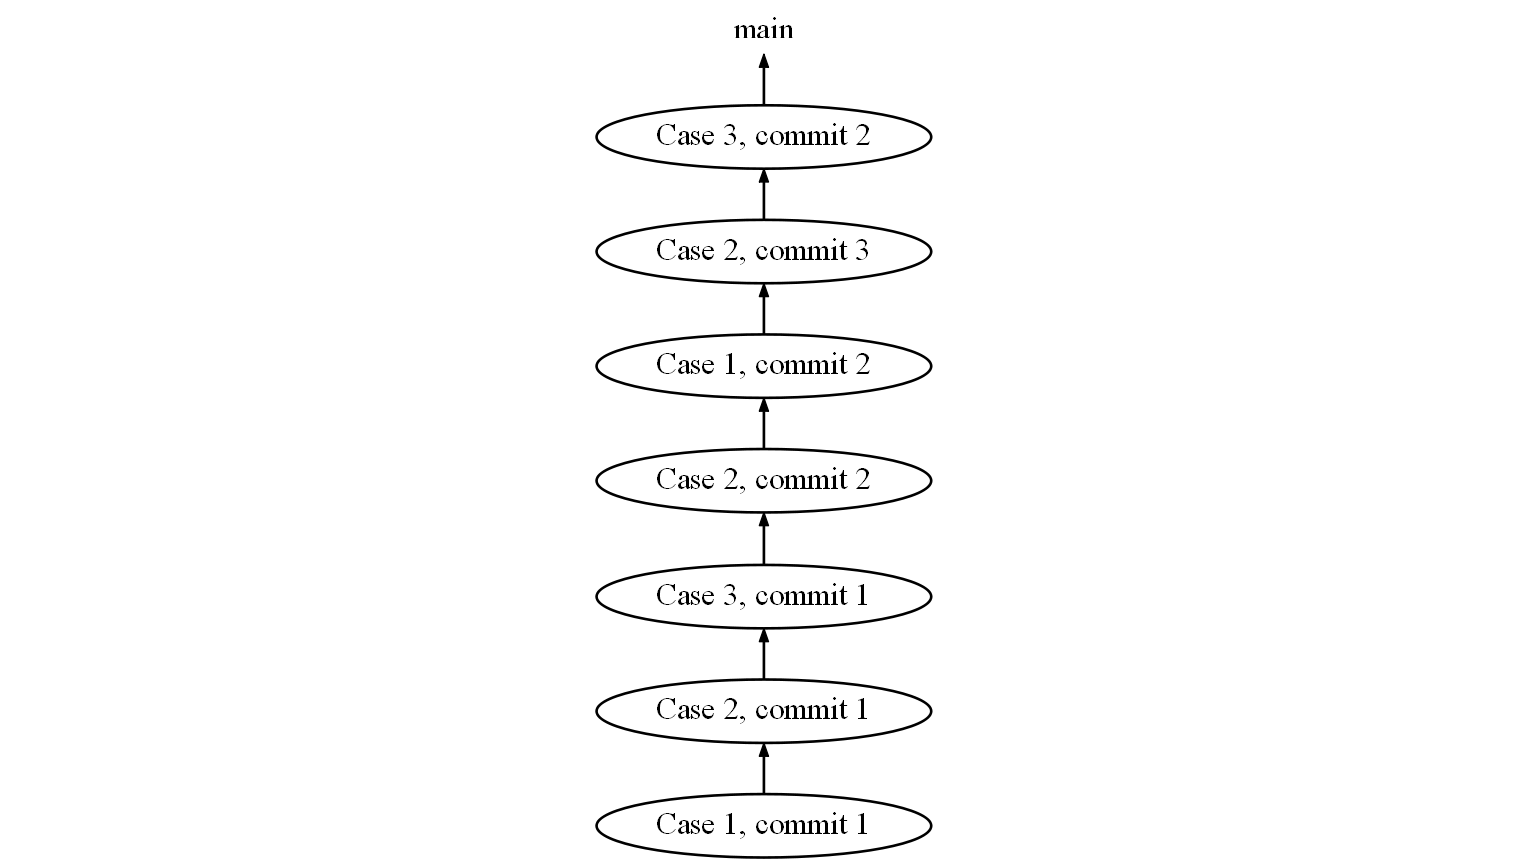
\includegraphics[scale=0.2]{02_2014_only-main.png}
\end{figure}

При ветвлении коммиты группируются по кейсам:
\begin{figure}[h!]
  \centering
  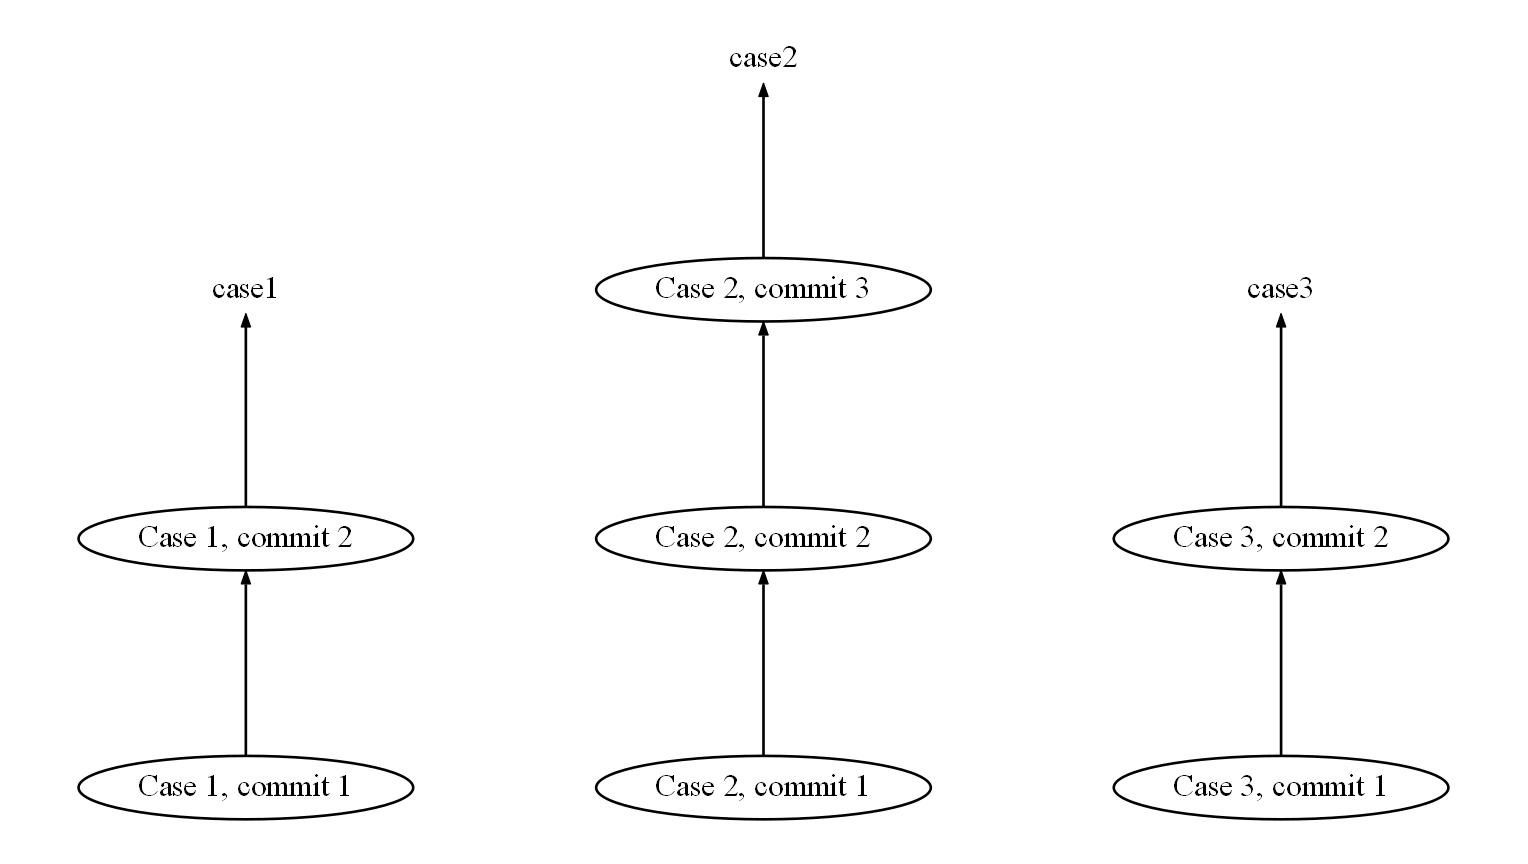
\includegraphics[scale=0.2]{02_2014_branches.png}
\end{figure}

\subsubsection*{Rebasing}

Rebasing может применяться в процессе работы над кейсом, а также для доставки коммитов в mainline.

Rebasing в процессе работы позволяет:

\begin{itemize}
  \item Получить ответвление от обновлённого mainline.
  \item Разрешать merge-conflicts небольшими порциями в ходе работы, а не одним большим куском в самом конце.
  \item Тестировать код своего кейса относительно нового mainline без его доставки в этот самый mainline.
\end{itemize}

Rebase вместо Merge как метод доставки кода в mainline позволяет получить:

\begin{itemize}
  \item Линейную историю в VCS. Линия проще и наглядней графа.
  \item Меньше проблем с blame, bisect и revert. Эти команды работают лучше на коммитах с одним родителем, чем с несколькими.
  \item Возможность удалять очень старые ветки (и их коммиты) из репозитория. Это повышает быстродействие репозитория. А если эти ветки всё-таки нужны "--- их можно хранить в архивном репозитории или в бэкапе. Тем, кто считает замедление репозитория при увеличении количества коммитов надуманной проблемой, есть смысл ознакомиться с исследованием Facebook \cite{Hlebnikov1}.
\end{itemize}

При доставке кода в mainline через Merge, mainline состоит в основном из merge-коммитов:
\begin{figure}[h!]
  \centering
  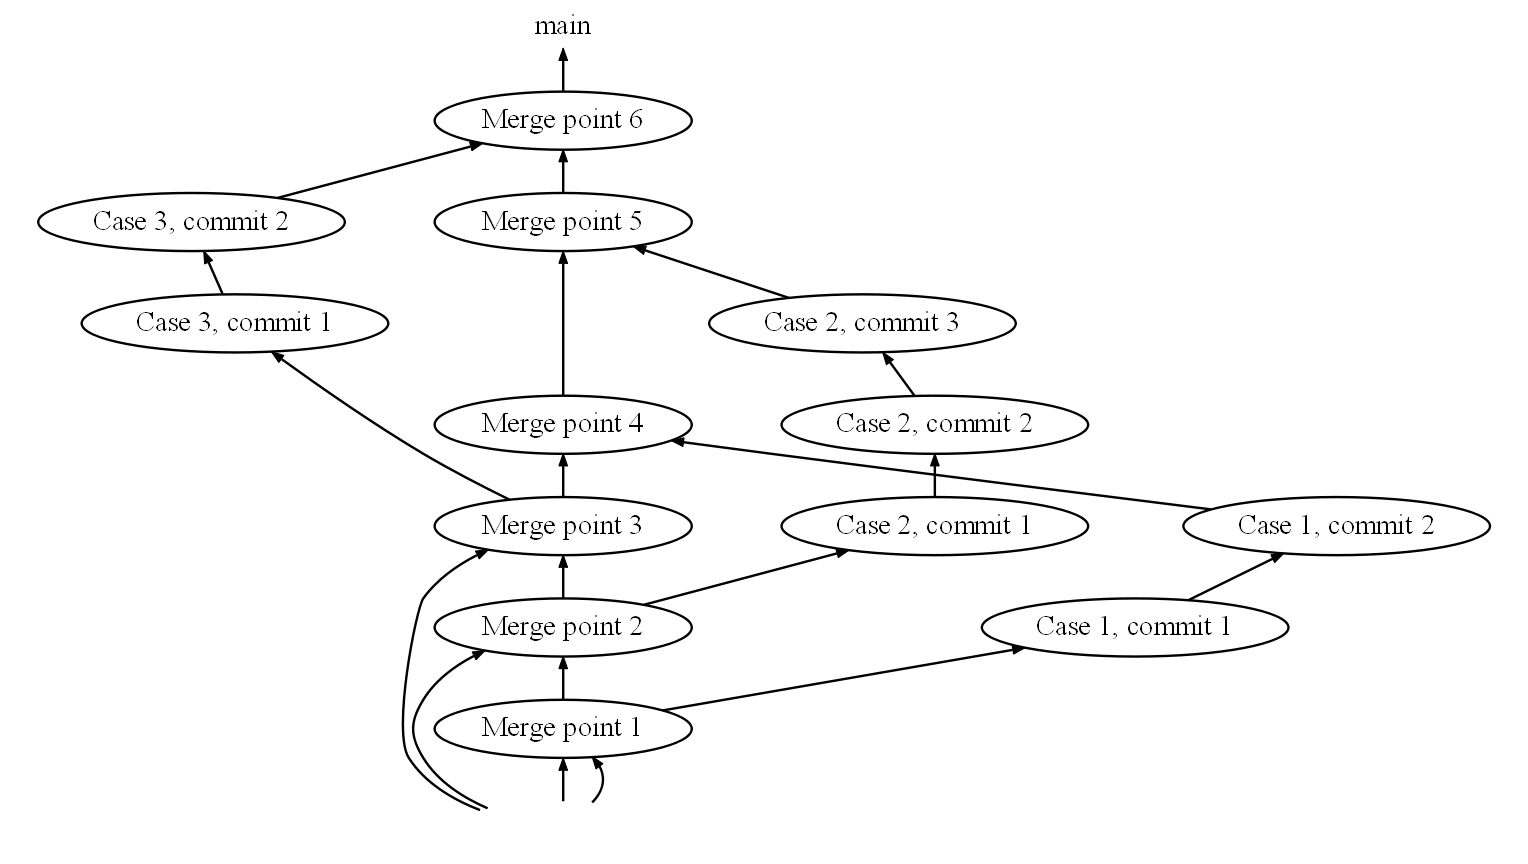
\includegraphics[scale=0.2]{02_2014_main-merged.png}
\end{figure}

Тот же самый граф, но без ярко выраженного вертикального mainline:
\begin{figure}[h!]
  \centering
  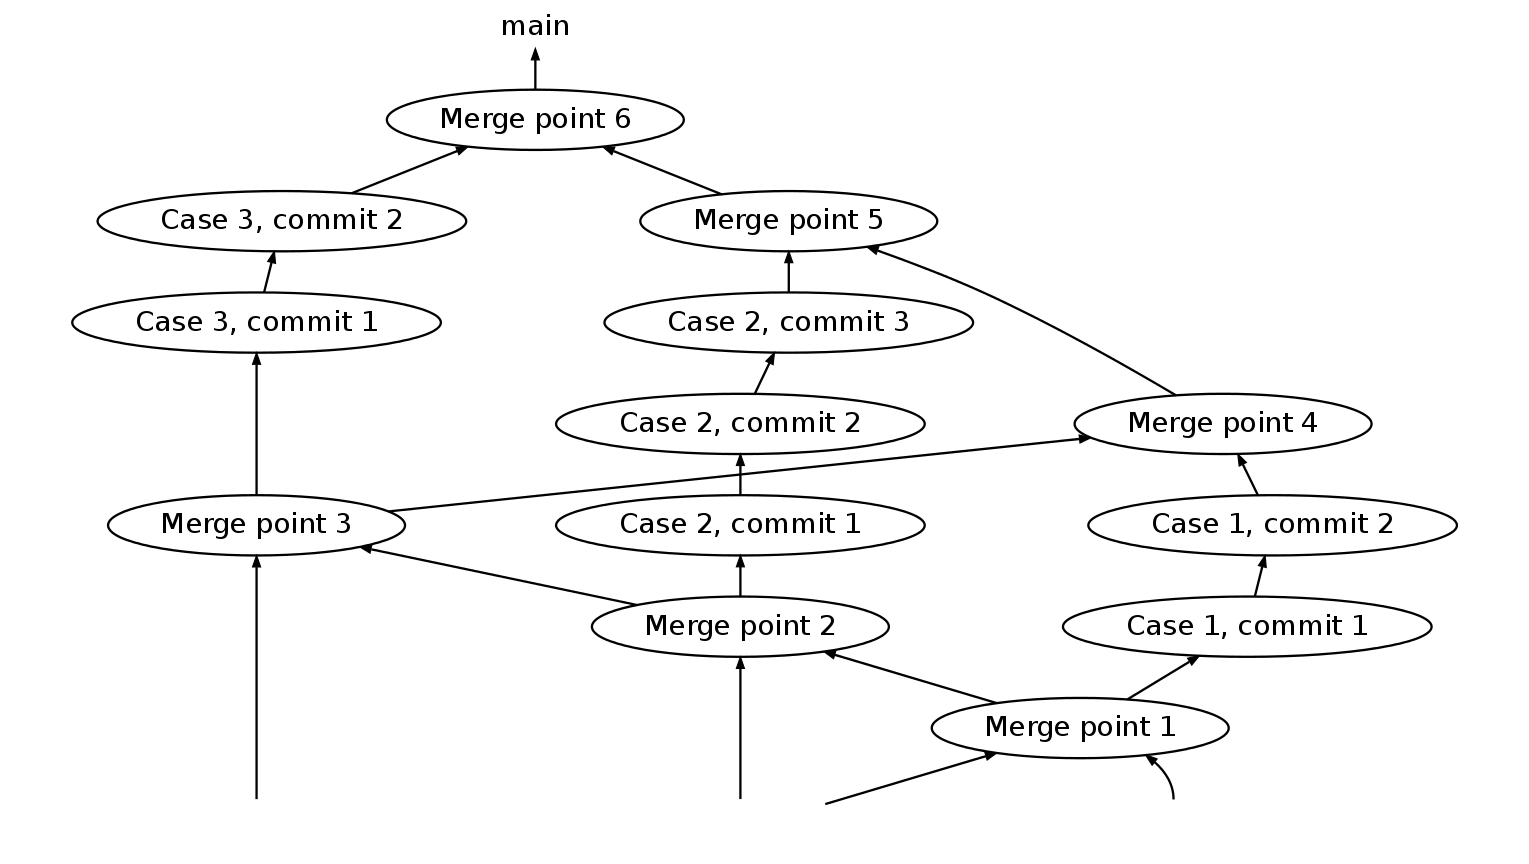
\includegraphics[scale=0.2]{02_2014_main-merged-weak-mainline.png}
\end{figure}

Как видно, в такой истории довольно трудно разобраться, особенно по прошествии долгого времени, или если разбирающийся "--- новый человек на проекте. В этом графе даже mainline трудно найти.

А вот история, которая получается при Rebase:
\begin{figure}[h!]
  \centering
  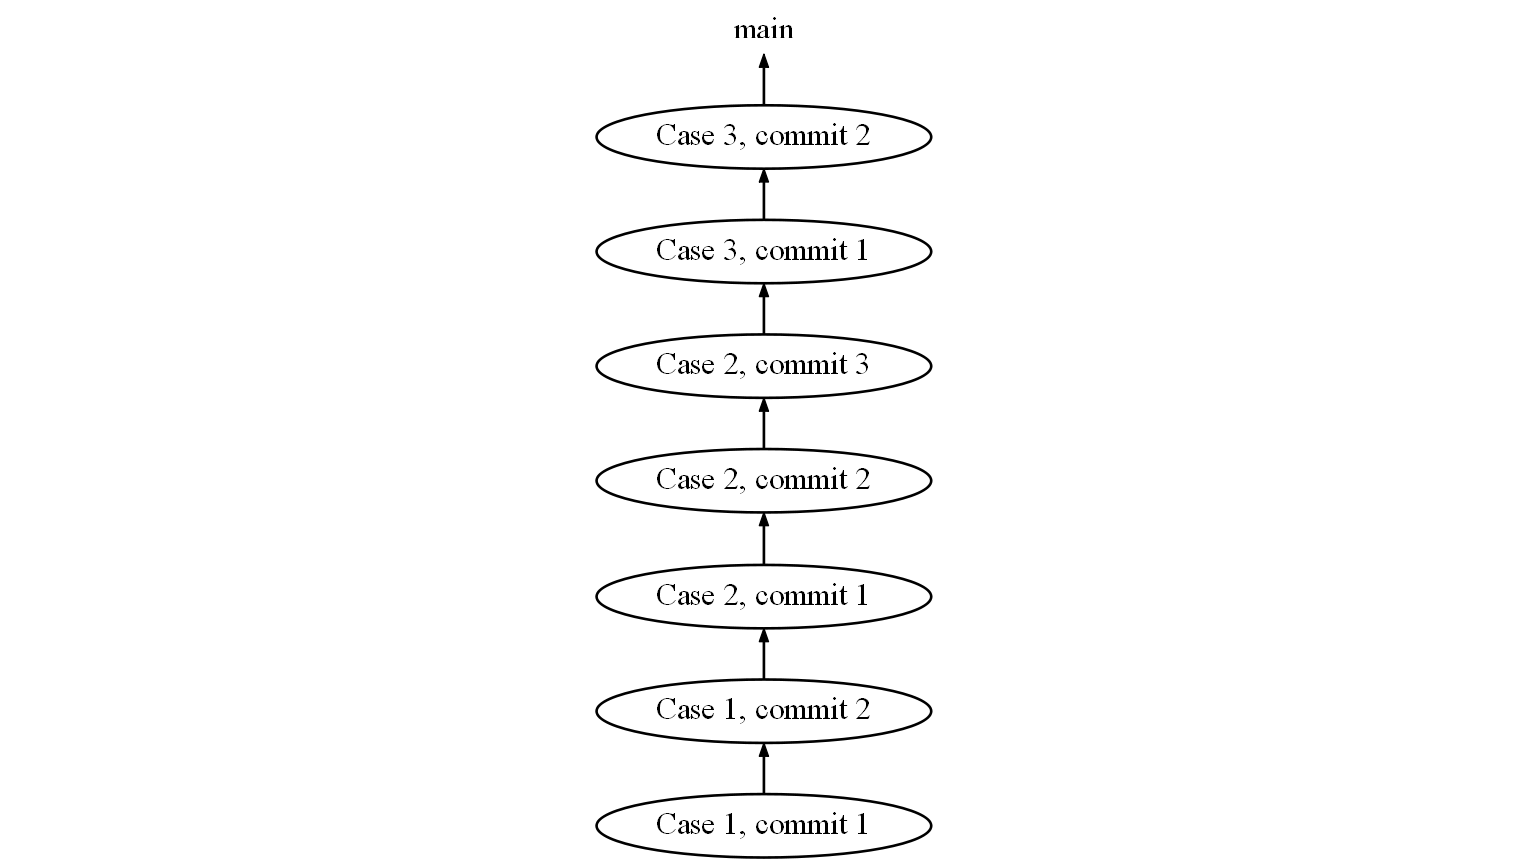
\includegraphics[scale=0.2]{02_2014_main-ordered.png}
\end{figure}

Как видно, история линейна, что сильно улучшает её читаемость. Но можно сделать ещё лучше "--- уменьшить количество коммитов. И в этом поможет squashing.

\subsubsection*{Squashing}

Squashing "--- это слияние нескольких коммитов в один. Squashing позволяет получить:

\begin{itemize}
  \item Компактную историю. Это тем важнее, чем дольше идёт разработка и чем больше коммитов собралось в репозитории.
  \item Меньше мусора в истории.
  \item Более лёгкий откат изменений.
\end{itemize}

Если после работы над кейсом ветка содержит много мусора в истории\ldots{}
\begin{figure}[h!]
  \centering
  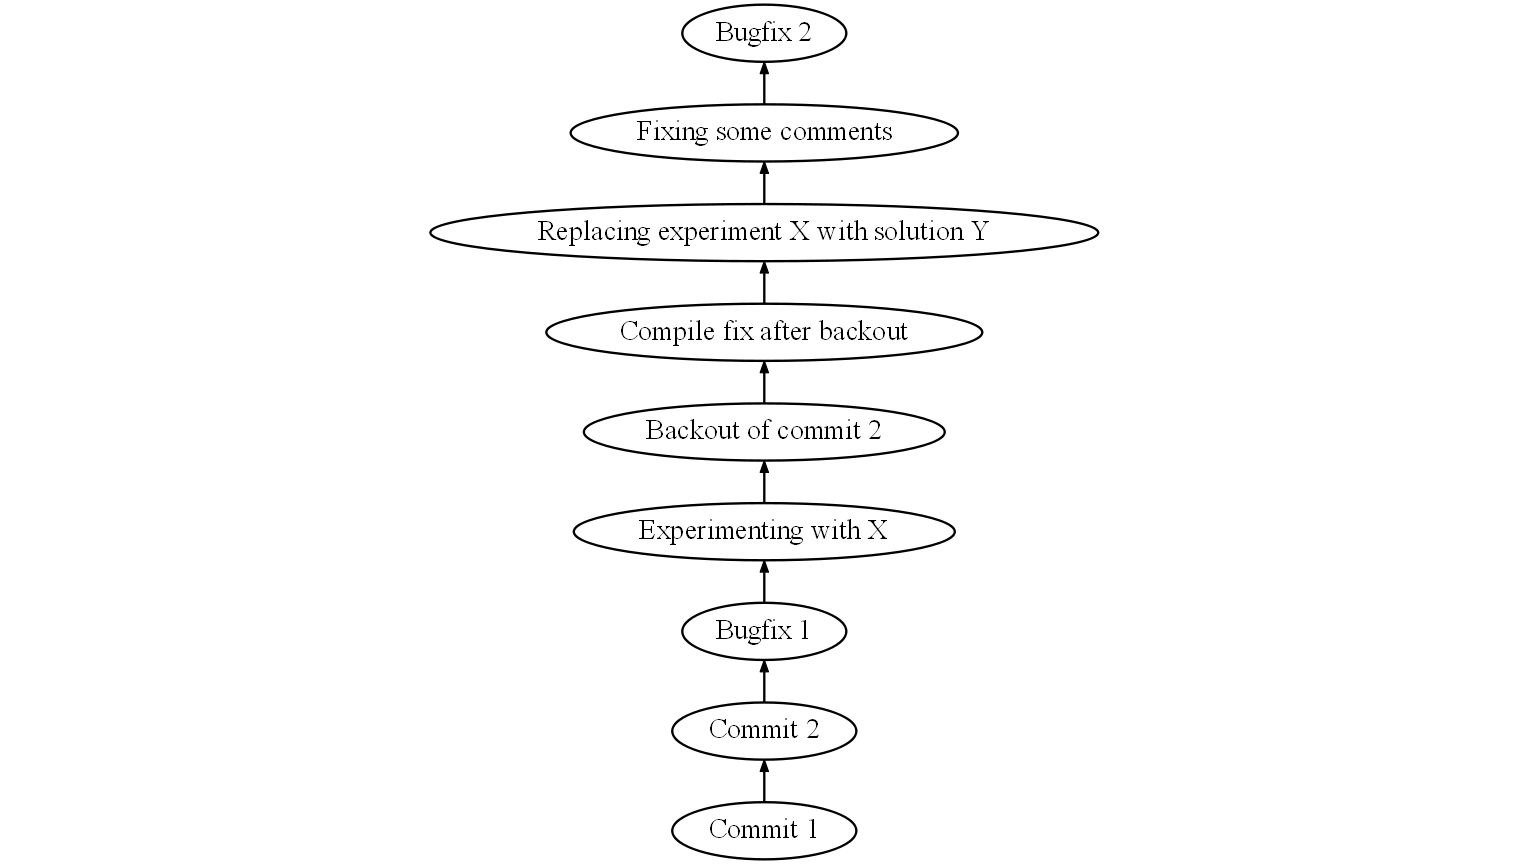
\includegraphics[scale=0.2]{02_2014_history-with-garbage.png}
\end{figure}

\ldots{}squashing позволит избавиться от этого мусора, слив все комиты в один:
\begin{figure}[h!]
  \centering
  
\includegraphics[scale=0.3]{02_2014_history-without-garbage.png}
\end{figure}

\subsection*{Конкретные команды, шаг за шагом}

Приведем примеры команд для Git и Mercurial в виде таблицы:

\begin{table}
  \centering
  \begin{tabular}{P{2.5cm}|P{3.5cm}|P{3.5cm}}
    \hline
                                  ~  & \textbf{Git}                   & \textbf{Mercurial}          \\ \hline
    Ответвление от mainline          & git checkout -{}-b case4       & hg book case4              \\
    Работа над кейсом                & git commit -m "Commit 1" \newline
                                       git commit -m "Commit 2" \ldots{}
                                                                    & hg commit -m "Commit 1" \newline
                                                                      hg commit -m "Commit 2" \ldots{} \\
    Rebase и squash              & git checkout -{}-b \emph{case4-2} \newline
                                   git rebase -{}-interactive main
                                                     & (нужны расширения rebase и histedit) \newline
                                                       hg rebase -{}-keep -{}-dest main \newline
                                                       hg histedit main \newline
                                                       hg book \emph{case4-2}      \\
    \hline
  \end{tabular}
\end{table}
Отдельно коснёмся «табу на rebase после push». Существует довольно распространённый миф, что если ветка запушена (push) на сервер "--- все возможности ребэйса (rebase) для неё потеряны, потому что если ветку проребэйсить и запушить на сервер опять (что возможно только с ключом --force), то это создаст несоответствие между репозиторием на сервере и репозиториями других разработчиков. В результате эти разработчики при попытке подтянуть эту ветку с сервера получат сломанную ветку.

На самом деле rebase возможен, если выполнять его правильно. На примере команд, приведённых в таблице, видно, что при ребэйсинге создаётся новая ветка, \textbf{case4-2}. Это принципиальный момент. Первоначальная ветка, \textbf{case4}, так и остаётся на своём месте, и получается аналог copy-on-write. Таким образом консистентность репозитория не нарушается, и ветка case4 не ломается "--- она просто устаревает. Теперь про неё можно забыть, а дальнейшую разработку, если она ещё продолжается, вести на ветке case4-2.

Также следует обратить внимание на ключ --interactive для Git и команду histedit для Mercurial. В результате их использования Git или Mercurial вызывают текстовый редактор, в котором разработчик может редактировать историю своей ветки: помечать коммиты для правки комментария, сливать несколько коммитов вместе, менять коммиты местами, удалять ненужные коммиты.

В сущности, многие коммиты "--- просто мусор в истории VCS: неудавшиеся эксперименты, багфиксы, фиксы компиляции, чистка неиспользуемых переменных, исправления опечаток в комментариях. Подобный материал в истории VCS не представляет ровным счётом никакого интереса. Как правило, от разработчика требуется имплементация фичи X или исправление бага Y, и желательно одним куском (то есть, как правило (хоть и не всегда), одним коммитом). А детали того, через что разработчик прошёл в процессе разработки, никого не интересуют. По этой причине мелкие правящие коммиты всегда имеет смысл объединить с «главными» коммитами, которые они дополняют. Это же относится и к фиксам в результате code review.

Делать слишком много «главных» коммитов для одного кейса тоже не имеет смысла. Наоборот, для большинства кейсов перед доставкой кода в mainline лучше слить все коммиты в один и использовать название кейса как комментарий этого единственного коммита. Если имел место рефакторинг без изменения функциональности "--- его имеет смысл выделить в отдельный коммит. Если имели место фиксы багов mainline'a, которые проявились при работе над данным кейсом "--- их тоже имеет смысл выделить в отдельные коммиты, и поместить эти коммиты перед основной разработкой. Других коммитов не нужно. Это и есть squashing "--- слияние нескольких коммитов в один.

Кроме чистки мусора в истории squashing также помогает убрать коммиты, которые не компилируются, путём слияния с фиксом компиляции. Это важно, если  используется bisect, а также в случае отката изменений.

Если вам захочется оставить в истории VCS свои чаяния и веяния по поводу данного кейса из ностальгических соображений "--- есть возможность сохранить их только для себя на той старой ветке case4, которая была любезно сохранена при copy-on-write-rebase. Не перетаскивая свой мусор в mainline, разработчик заодно не создает аналогичного искушения для товарищей по команде.

\subsection*{Доставка кода в mainline}

Итак, работа над кейсом завершена, код кейса оттестирован с новейшим mainline. После финальных rebase и squash на ветке должна находиться краткая и красивая история кейса, а сама ветка основана на верхушке mainline. Это и есть подходящий момент для доставки кода кейса в mainline. Для этого надо всего лишь переместить указатель mainline вперёд по ветке case4-2 "--- сделать fast-forward. Это можно сделать несколькими способами; автор предпочитает такие:

\begin{table}
  \centering
  \begin{tabular}{P{3.5cm}|P{6cm}} \hline
    \textbf{Git}                       & \textbf{Mercurial}            \\ \hline
     git push . case4-2:main      & (hg update case4-2) \linebreak
                               hg book main \linebreak  \# «book» does fast-forward \linebreak
                               \# in this case                                               \\ \hline
  \end{tabular}
\end{table}
Важно обратить внимание на точку после git push. Она означает «текущий репозиторий». Однако можно пушить и сразу в origin:

git push origin case4-2:main

При этом не следует опасаться поломки origin/main, т.к. если предлагаемый push не fast-forward, Git не позволит выполнить push без ключа -{}-force.

\subsection*{Выводы}

В результате использования предложенного подхода мы получаем:

\begin{itemize}
  \item Удобство разработки на отдельных ветвях.
  \item Возможность всегда работать и тестировать свои изменения относительно новейшего mainline.
  \item Линейную историю.
  \item Группировку коммитов по кейсам.
  \item Безупречную и компактную историю без мусора.
\end{itemize}

\begin{figure}[h!]
  \centering
  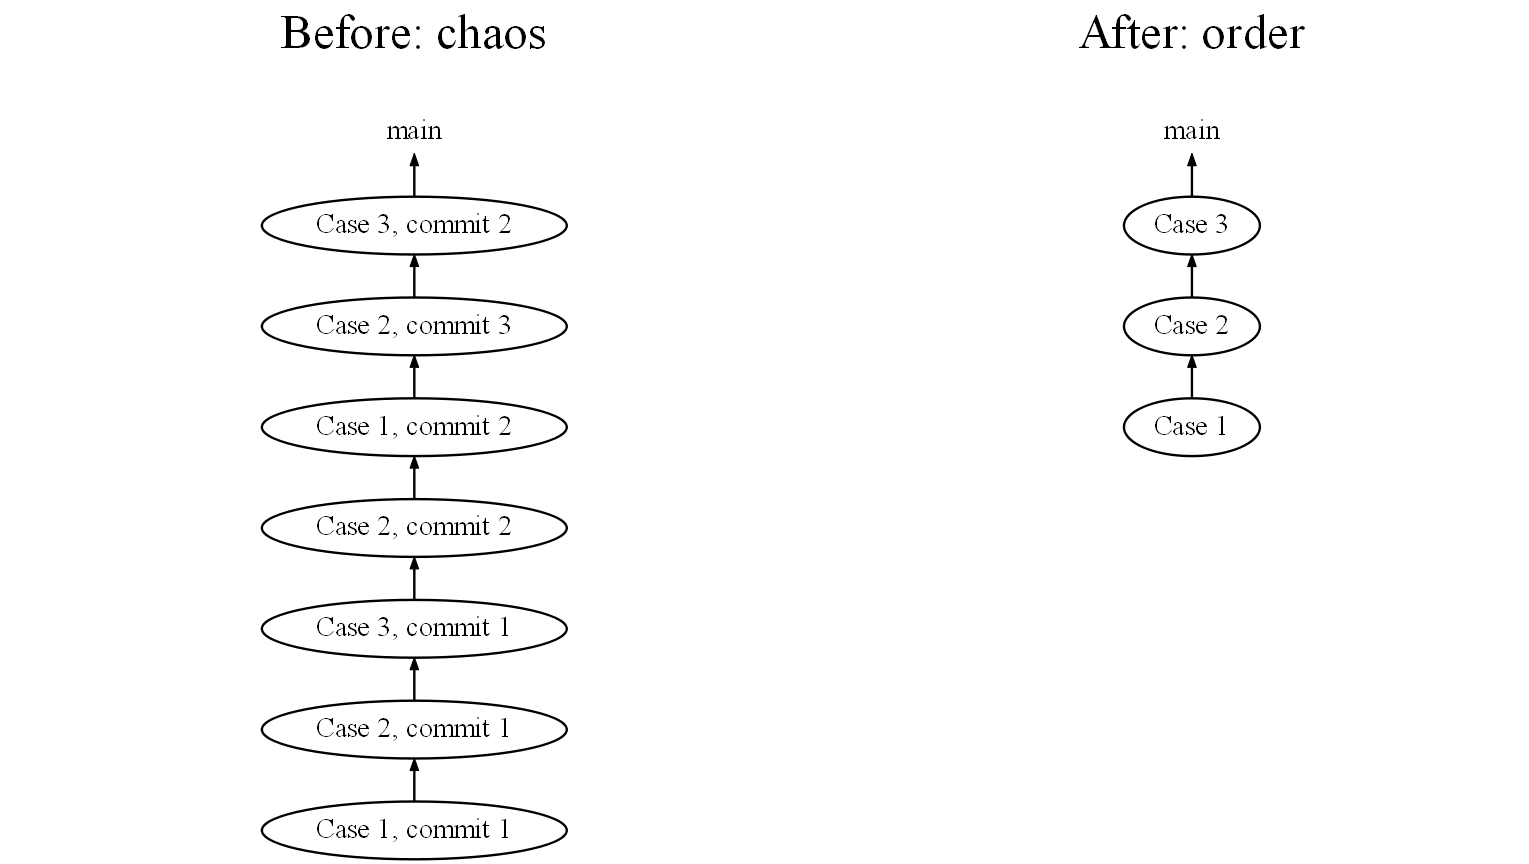
\includegraphics[scale=0.2]{02_2014_before-vs-after.png}
\end{figure}

\begin{thebibliography}{9}
\bibitem{Hlebnikov1} \url{http://thread.gmane.org/gmane.comp.version-control.git/189776}
\end{thebibliography}
\end{document}

%%%\chapter{LVEE Winter 2014}
\documentclass[10pt, a5paper]{article}
\usepackage{pdfpages}
\usepackage{parallel}
\usepackage[T2A]{fontenc}
\usepackage{ucs}
\usepackage[utf8x]{inputenc}
\usepackage[polish,english,russian]{babel}
\usepackage{hyperref}
\usepackage{rotating}
\usepackage[inner=2cm,top=1.8cm,outer=2cm,bottom=2.3cm,nohead]{geometry}
\usepackage{listings}
\usepackage{graphicx}
\usepackage{wrapfig}
\usepackage{longtable}
\usepackage{indentfirst}
\usepackage{array}
\newcolumntype{P}[1]{>{\raggedright\arraybackslash}p{#1}}
\frenchspacing
\usepackage{fixltx2e} %text sub- and superscripts
\usepackage{icomma} % коскі ў матэматычным рэжыме
\PreloadUnicodePage{4}

\newcommand{\longpage}{\enlargethispage{\baselineskip}}
\newcommand{\shortpage}{\enlargethispage{-\baselineskip}}

\def\switchlang#1{\expandafter\csname switchlang#1\endcsname}
\def\switchlangbe{
\let\saverefname=\refname%
\def\refname{Літаратура}%
\def\figurename{Іл.}%
}
\def\switchlangen{
\let\saverefname=\refname%
\def\refname{References}%
\def\figurename{Fig.}%
}
\def\switchlangru{
\let\saverefname=\refname%
\let\savefigurename=\figurename%
\def\refname{Литература}%
\def\figurename{Рис.}%
}

\hyphenation{admi-ni-stra-tive}
\hyphenation{ex-pe-ri-ence}
\hyphenation{fle-xi-bi-li-ty}
\hyphenation{Py-thon}
\hyphenation{ma-the-ma-ti-cal}
\hyphenation{re-ported}
\hyphenation{imp-le-menta-tions}
\hyphenation{pro-vides}
\hyphenation{en-gi-neering}
\hyphenation{com-pa-ti-bi-li-ty}
\hyphenation{im-pos-sible}
\hyphenation{desk-top}
\hyphenation{elec-tro-nic}
\hyphenation{com-pa-ny}
\hyphenation{de-ve-lop-ment}
\hyphenation{de-ve-loping}
\hyphenation{de-ve-lop}
\hyphenation{da-ta-ba-se}
\hyphenation{plat-forms}
\hyphenation{or-ga-ni-za-tion}
\hyphenation{pro-gramming}
\hyphenation{in-stru-ments}
\hyphenation{Li-nux}
\hyphenation{sour-ce}
\hyphenation{en-vi-ron-ment}
\hyphenation{Te-le-pathy}
\hyphenation{Li-nux-ov-ka}
\hyphenation{Open-BSD}
\hyphenation{Free-BSD}
\hyphenation{men-ti-on-ed}
\hyphenation{app-li-ca-tion}

\def\progref!#1!{\texttt{#1}}
\renewcommand{\arraystretch}{2} %Іначай формулы ў матрыцы зліпаюцца з лініямі
\usepackage{array}

\def\interview #1 (#2), #3, #4, #5\par{

\section[#1, #3, #4]{#1 -- #3, #4}
\def\qname{LVEE}
\def\aname{#1}
\def\q ##1\par{{\noindent \bf \qname: ##1 }\par}
\def\a{{\noindent \bf \aname: } \def\qname{L}\def\aname{#2}}
}

\def\interview* #1 (#2), #3, #4, #5\par{

\section*{#1\\{\small\rm #3, #4. #5}}

\def\qname{LVEE}
\def\aname{#1}
\def\q ##1\par{{\noindent \bf \qname: ##1 }\par}
\def\a{{\noindent \bf \aname: } \def\qname{L}\def\aname{#2}}
}

\switchlang{be}
\begin{document}
\title{Свой уласны Dropbox, з календаром, кантактамі і RSS\footnote{\url{andrej@zahar.ws}, \url{http://lvee.org/ru/abstracts/169}}}
\author{Андрэй Захарэвіч, Мінск, Belarus}
\maketitle
\begin{abstract}
This is a story of attempt to get some open source and provider independent solutions, namely ownCloud, for tasks we usually allow to perform companies and corporations like Dropbox Inc. or Google Inc. 
\end{abstract}
\section*{Папярэджанне}

Ад пачатку хацеў бы заўважыць, што гэта не спроба разглядзець усе магчымасці ownCloud. Гэта расказ пра прымяненне яго як інструмента для задавальнення пэўных (маіх) патрэб такім чынам, каб гэты было зручна мне.

\section*{Мэты і задачы}

Пачнем, вядома ж, з вызначэння задач і таго, наколькі абраны інструмент дазваляе іх выканаць.

\subsection*{Файлаабменнік}

Задачы:

\begin{itemize}
  \item Магчымасць падзяліцца спасылкай на нейкі файл з кім заўгодна (з нейкім механізмам абмежавання доступа);
  \item Магчымасць стварыць агульны набор рэсурсаў для некалькіх карытальнікаў
  \item Звычайныя магчымасці па абнаўленню файлаў з адной крыніцы на ўсе месцы, дзе ляжыць яго копія
  \item Кліент пад Linux для сінхранізацыі ўсяго акаўнта ці асобных яго папак. Пажадана, каб дазваляў дадаваць некалькі акаўнтаў.
\end{itemize}

\subsection*{Кантакты і календар}

\begin{itemize}
  \item Цэнтралізаванае сховішча для календара і кантактаў
  \item З магчымасцю сінхранізацыі на прылады Android. У ідэале каб сінханізацыя адбывалася гэтак жа, як са звычайнымі правайдэрамі, то бок как не абмяжоўваць спіс праграм, якія потым з гэтымі кантактамі ці календарнымі запісамі змогуць працаваць
  \item Зручны (хаця б мінімальна) інтэрфейс для кампьютэра з магчымасцю аб'ядноўваць кантакты ў групы.
  \item Групы кантактаў павінны быць бачныя і даступныя для любых аперацый як з кампа, так і з тэлефона.
  \item Магчымасць імпарту кантактаў і календара ў Thunderbird
  \item Магчымасць экспарту у файл і пераносу на іншы сервер
\end{itemize}

\subsection*{RSS}

\begin{itemize}
  \item Магчымасць чытаць як з кампьютэра, так і з Android-прылад
  \item Магчымасць дадаваць з кампьютэра і андроід-прылад
  \item Магчымасць сінхранізаваць стан (прачытаны, пазначаны як цікавы) для розных крыніц
  \item У ідэале, магчымасць атырмаць доступ праз вэб-інтэрфейс
  \item Магчымасць экспарту у файл і пераносу на іншы сервер
\end{itemize}

\subsection*{Спасылкі}

\begin{itemize}
  \item Магчымасць чытаць як з кампьютэра, так і з Android-прылад
  \item Магчымасць дадаваць з кампьютэра і андроід-прылад
  \item Групіроўка па групах ці тэгах, даступная для ўсіх кліентаў
  \item Магчымасць экспарту у файл і пераносу на іншы сервер
\end{itemize}

\section*{Як атрымаць уласнае воблака ад пачатку да канца}

Тут я паспрабую караценька расказаць, як можна атырмаць усё што я шукаў ва ўласным воблачным сховішчы.

\subsection*{Як паставіць ownCloud}

Самы просты варыянт атрымання інстансу ownCloud "--- гэта паставіць яго, карыстаючыся парадамі з афіцыйнага кіраўніцтва да бягучай стабільнай версіі  \cite{zahar1}.

Калі караценька: узяць гатовы пакет да большасці папулярных дыстрыбутываў, ці можна нават прапісаць адпаведную крыніцы для інсталяцыі пакетаў. Другі спосаб дазваляе даволі зручна абнаўляцца. Я такім чынам перажыў ужо нават апдэйт паміж мажорнымі версіямі.

\subsection*{Парады па наладцы}

Працягваючы слаўную традыцыю, прапаную звярнуцца да парад па інсталяцыі \cite{zahar1} i настройцы базы дадзеных \cite{zahar4}.

Хаця сам я спрабаваў сёе-тое з прыведзеных парад, але вымушаны заўважыць, што на серверы з не надта вялікім аб'ёмам памяці кэш можа не паскараць працу, а замаруджваць яе, насуперак парадам з афіцыйнага кіраўніцтва. А неправільная настройка PHP-кэшавання можа зрабіць вашае воблака бясконца бяспечным (то бок, недаступным нікому).

Даволі неблага працуе выкананне задач па раскладзе з дапамогай cron-задач, хаця, нажаль, некаторыя задачы могуць павісаць. У выпадку з RSS калі працэс не здолее атрымаць абнаўленні за пэўны час і перастане працаваць не знішчыўшчы lock-файл, то абнаўленне будзе немагчымае без таго, каб гэты файл знішчыць. Гэта магчыма зрабіць рукамі, альбо натравіць асобны скрыпт, які будзе па раскладзе маніторыць стан працэсу.

Калі вы плануеце карыстацца вэб-інтэрфейсам каб дадаваць файлы ў воблака, то варта будзе яшчэ выканаць дадатковыя настройкі для гэтага \cite{zahar6}. Паколькі мне дастаткова якіх 150--250 мегабайтаў, то хапіла проста настройкі адпаведных зменных у настройках PHP.

Што сапраўды варта зрабіць, гэта настройка бяспекі. Зноўку ж, варта звярнуцца да адпаведнага раздзелу афіцыйнага кіраўніцтва \cite{zahar3}. Вельмі раю адключыць доступ не па HTTPS і выканаць іншыя парады. З дапамогай гэтых мер я змог падняць сайт па рэйтынгу SSL Server Test \cite{zahar5} ад T(\textbackslash{}C) да T(A).

Але з любымі мерамі бяспекі варта помніць: калі вы нешта публікуеце ў інтэрнэце, то даць стопрацэнтную гарантыю таго, што інфармацыя будзе даступная толькі і выключна вам ужо немагчыма. Але не варта панікаваць.

\subsection*{Перанос дадзеных ва ўласнае воблака}

Прасцей за ўсё з файламі: перанос можна пачаць адразу ж, выкарыстоўваючы вэб-інтэрфейс. Ці дэсктопны кліент \cite{zahar7}. Калі вы вышкталцоны аматар рэдкіх вычварэнняў і надзвычайных прыгод, то можна скарыстацца і мабільным кліентам \cite{zahar8}. Уласна, карыстацца можна з дапамогай таго ж заапарку. Дэсктопныя кліенты з нядаўніх часоў дазваляюць сінхранізацыю з некалькімі акаўнтамі.

Кантакты я пераносіў шляхом экспарту з Google Contacts і \linebreak паўторным імпартам ужо ў ownCloud. Калі вы ўсё яшчэ карыстаеццеся кірыліцай і іншым састарэлым юнікодам па-за межамі ASCII, то я б параіў выбіраць фармат vCard, інакш будуць праблемы з кадзіроўкаю. Ну і каб закрыць пытанні з кадзіроўкаю: выкарыстанне знакаў у імёнах груп кантактаў недапушчальнае "--- у выніку дзе-небудзь пасля сінхранізацыі імёны будуць ламацца. Давялоса міграваць групу <<Сям'я>> у групу <<Сваякі>>.

Калі вы "--- як і я "--- прасцей запамінаеце твары асоб чым імёны, то для вас благая навіна: выявы для кантактаў вы страціце. А вось для аматараў усё акуратна раскладаць па папачках і каталагізаваць у мяне добрая навіна: кантакты фактычна не належаць да нейкай групы, яны проста маюць адпаведны тэг. То бок, калі у вас сябар, з якім вы разам працавалі на нейкую кампанію, займаліся спортам і падзяляеце захапленне Linux, прычым для кожнай прыгаданай прыкметы ў вас ёсць асобная група, то гэты ваш знаёмы можа патрапіць у чатыры ці болей груп. Пацешце ўнутранага бюракрата!

На гэтым месцы лепш за ўсё настроіць двухбаковую сінхранізацыю з нейкім Android-смартфонам ці планшэтам. Добрая навіна: пачынаючы з версіі 4.0 Андроід дазваляе дадаваць правайдэры кантактаў і календара. Я спрабаваў карыстацца рознымі праграмамі, але DAVdroid – CalDAV/CardDAV Sync паказаў сябе лепш за ўсё: сіхранізацыя працуе хутка і надзейна. Дазваляе сінхранізаваць адразу кантакты і календар. Перажыў некалькі абнаўленняў як воблака, так і сваіх уласных.

З календаром было крыху больш складана: я не знайшоў спосабу штатным чынам экспартаваць яго з гуглаўскага календара. Я скарыстаўся метадам з блога Man and Keyboard \cite{zahar9}. Калі караценька:

\begin{enumerate}
  \item Выдаліць непатрэбныя падзеі
  \item Настроіць двухбаковую сінхранізацыю календара паміж \linebreak Android-прыладай і ownCloud
  \item Скрыстацца праграмай iCal Import/Export CalDAV \cite{zahar10} і перанесці сінхранізаваць календар паміж аблокамі
\end{enumerate}

Ну і раз ужо усё гэта так удала сінхранізавалася, то можна сінхранізаваць з дэсктопам \cite{zahar12, zahar13}.

RSS-чыталка пакуль мне лепш за ўсё спадабалася адна  \cite{zahar14}, якая дазваляе зручна чытаць і сінхранізаваць. Нажаль, у сэнсе кіравання падпіскамі па-за межамі дадаць новую крыніцу лепш карыстацца веб-інтэрфейсам. Але, з іншага боку, карыстацца веб-інтэрфейсам для чытання не так зручна.

Са спасылкамі прасцей за ўсё: карыстацца праз веб-інтэрфейс досыць зручна. Ёсць неблагі кліент Андроід \cite{zahar15}. Нажаль, кліент не дазваляе дадаваць групы для спасылак і рэдагаваць спасылкі. Ва ўсім астатнім кліент досыць зручны (і невялікі).

Усе функцыі былі рэалізаваныя праз штатныя плагіны.

\begin{thebibliography}{99}
\bibitem{zahar1} ownCloud 9.0 Server Administration Manual: Installation. \url{https://doc.owncloud.org/server/8.2/admin_manual/installation/index.html}
\bibitem{zahar2} ownCloud Server Administration Manual:Server Tuning \& Performance Tips. \url{https://doc.owncloud.org/server/8.2/admin_manual/configuration_server/performance_tuning.html}
\bibitem{zahar3} ownCloud Server Administration Manual: Hardening and Security Guidance. \url{https://doc.owncloud.org/server/8.2/admin_manual/configuration_server/harden_server.html?highlight=security}
\bibitem{zahar4} ownCloud Server Administration Manual: Database Configuration. \url{https://doc.owncloud.org/server/8.2/admin_manual/configuration_database/linux_database_configuration.html}
\bibitem{zahar5} Qualys SSL Labs SSL Server Test. \url{https://www.ssllabs.com/ssltest/}
\bibitem{zahar6} ownCloud Server Administration Manual: Uploading big files. \url{https://doc.owncloud.org/server/8.2/admin_manual/configuration_files/big_file_upload_configuration.html}
\bibitem{zahar7} ownCloud Desktop Clients. \url{https://owncloud.com/products/desktop-clients/}
\bibitem{zahar8} ownCloud client for Android. \url{https://play.google.com/store/apps/details?id=com.owncloud.android}
\bibitem{zahar9} Man and Keyboard: Google to Owncloud, Contacts and Calendar. \url{http://manandkeyboard.tk/2015/02/26/google-to-owncloud-contacts-and-calendar/}
\bibitem{zahar10} iCal Import/Export CalDAV. \url{https://play.google.com/store/apps/details?id=tk.drlue.icalimportexport}
\bibitem{zahar11} DAVdroid – CalDAV/CardDAV Sync. \url{https://play.google.com/store/apps/details?id=at.bitfire.davdroid}
\bibitem{zahar12} Moving your Contacts and Calendar Away from Google. \url{http://flailingmonkey.com/moving-contacts-calendar-google/}
\bibitem{zahar13} Birthday Calendar with ownCloud via CalDAV. \url{http://blog.mehl.mx/2014/birthday-calendar-with-owncloud-via-caldav/}
\bibitem{zahar14} ownCloud News Reader. \url{https://play.google.com/store/apps/details?id=de.luhmer.owncloudnewsreader}
\bibitem{zahar15} ownCloud Bookmarks. \url{https://play.google.com/store/apps/details?id=cz.nethar.owncloudbookmarks}
\end{thebibliography}

\end{document}

\documentclass[10pt, a5paper]{article}
\usepackage{pdfpages}
\usepackage{parallel}
\usepackage[T2A]{fontenc}
\usepackage{ucs}
\usepackage[utf8x]{inputenc}
\usepackage[polish,english,russian]{babel}
\usepackage{hyperref}
\usepackage{rotating}
\usepackage[inner=2cm,top=1.8cm,outer=2cm,bottom=2.3cm,nohead]{geometry}
\usepackage{listings}
\usepackage{graphicx}
\usepackage{wrapfig}
\usepackage{longtable}
\usepackage{indentfirst}
\usepackage{array}
\newcolumntype{P}[1]{>{\raggedright\arraybackslash}p{#1}}
\frenchspacing
\usepackage{fixltx2e} %text sub- and superscripts
\usepackage{icomma} % коскі ў матэматычным рэжыме
\PreloadUnicodePage{4}

\newcommand{\longpage}{\enlargethispage{\baselineskip}}
\newcommand{\shortpage}{\enlargethispage{-\baselineskip}}

\def\switchlang#1{\expandafter\csname switchlang#1\endcsname}
\def\switchlangbe{
\let\saverefname=\refname%
\def\refname{Літаратура}%
\def\figurename{Іл.}%
}
\def\switchlangen{
\let\saverefname=\refname%
\def\refname{References}%
\def\figurename{Fig.}%
}
\def\switchlangru{
\let\saverefname=\refname%
\let\savefigurename=\figurename%
\def\refname{Литература}%
\def\figurename{Рис.}%
}

\hyphenation{admi-ni-stra-tive}
\hyphenation{ex-pe-ri-ence}
\hyphenation{fle-xi-bi-li-ty}
\hyphenation{Py-thon}
\hyphenation{ma-the-ma-ti-cal}
\hyphenation{re-ported}
\hyphenation{imp-le-menta-tions}
\hyphenation{pro-vides}
\hyphenation{en-gi-neering}
\hyphenation{com-pa-ti-bi-li-ty}
\hyphenation{im-pos-sible}
\hyphenation{desk-top}
\hyphenation{elec-tro-nic}
\hyphenation{com-pa-ny}
\hyphenation{de-ve-lop-ment}
\hyphenation{de-ve-loping}
\hyphenation{de-ve-lop}
\hyphenation{da-ta-ba-se}
\hyphenation{plat-forms}
\hyphenation{or-ga-ni-za-tion}
\hyphenation{pro-gramming}
\hyphenation{in-stru-ments}
\hyphenation{Li-nux}
\hyphenation{sour-ce}
\hyphenation{en-vi-ron-ment}
\hyphenation{Te-le-pathy}
\hyphenation{Li-nux-ov-ka}
\hyphenation{Open-BSD}
\hyphenation{Free-BSD}
\hyphenation{men-ti-on-ed}
\hyphenation{app-li-ca-tion}

\def\progref!#1!{\texttt{#1}}
\renewcommand{\arraystretch}{2} %Іначай формулы ў матрыцы зліпаюцца з лініямі
\usepackage{array}

\def\interview #1 (#2), #3, #4, #5\par{

\section[#1, #3, #4]{#1 -- #3, #4}
\def\qname{LVEE}
\def\aname{#1}
\def\q ##1\par{{\noindent \bf \qname: ##1 }\par}
\def\a{{\noindent \bf \aname: } \def\qname{L}\def\aname{#2}}
}

\def\interview* #1 (#2), #3, #4, #5\par{

\section*{#1\\{\small\rm #3, #4. #5}}

\def\qname{LVEE}
\def\aname{#1}
\def\q ##1\par{{\noindent \bf \qname: ##1 }\par}
\def\a{{\noindent \bf \aname: } \def\qname{L}\def\aname{#2}}
}

\begin{document}
\title{Обзор решений на рынке открытого ПО для создания СХД\footnote{\url{alex_kls@mail.ru}, \url{http://lvee.org/ru/abstracts/181}}}
\author{Александр Клыга, Минск, Беларусь}
\maketitle
\begin{abstract}
The survey of possible data storage solutions based on Open Source programs is presented. We focus on the ZFS file system and available solutions for data storage along with the direct-attached storage model. In addition, solutions to form data stora\-ge by using network-attached storage and storage area networks are outlined. Eventually, a review of  cluster data storage on the basis of the storage object files system is considered.
\end{abstract}
Создание эффективного хранилища данных "--- одна из сложных задач для системного архитектора и системного администратора, которому предстоит им управлять, и поэтому неудивительно, что \linebreakочень часто эти две разные роли объединяются в одном лице. Именно ему приходится выбирать решение, способное эффективно решать поставленные задачи, и когда ограниченность ресурсов не дает возможности приобретения дорогих решений от ведущих вендоров в производстве систем хранения данных, выходом из подобной ситуации зачастую является использование решений с открытым программным обеспечением на базе операционных систем Linux.

Операционная система Linux с ее открытым кодом в сочетании с широкими возможностями поддержи различных аппаратных платформ и программных продуктов Open Source идеально подходит для создания эффективных систем хранения данных СХД любой сложности. Ниже представлен обзор нескольких таких решений.

Первое решение "--- программный продукт на базе дистрибутива Debian OpenMediaVault (официальный сайт проекта \linebreak\url{openmediavault.org}), ориентированный на создание СХД модели NAS. Включает в себя программный RAID (0, 1, 5, 6, 10, JBOD), почтовый клиент, SSH, FTP, SMB/CIFS, NFS, RSYNC, средства управления пользователями и  мониторинга работы. Возможности OMV могут быть расширены плагинами, например, такими как DAAP-медиа-сервер, ISCSI, BitTorrent-клиент и другими. В настоящий момент разработка и развитие OMV версии 2 приостановлена (последняя стабильная версия 2.1), и  полным ходом идет  работа над новой версией OMV 3.0 с кодовым названием ``Erasmus'' (данная версия в качестве beta доступна для скачивания и установки). Ключевой особенностью 3-й версии OMV станет адаптация проекта под новую версию Debian 8 и расширение возможностей за счет переработки старых и выпуска новых плагинов. В качестве ключевых особенностей данного дистрибутива также можно отметить многоязычность (включая поддержку русского языка), поддержку GPT и файловых систем ext4/XFS/JFS, неплохой web-интерфейс. Руководит проектом Волкер Тейле (Volker Theile), бывший основной разработчик FreeNAS.

Следующее решение в обзоре "--- проект openfiler (официальный сайт проекта \url{www.openfiler.com}), основанный на интересном дистрибутиве rPATH Linux. В настоящий момент для скачивания  доступна версия 2.99. Ключевой особенностью данного проекта является возможность создания СХД моделей NAS/SAN с поддержкой интерфейсов FC (Fibre Channel) и iSCSI большой емкости (более 60TB). Openfiler поддерживает cсоздание и обслуживание программных RAID-массивов различных уровней (0,1,5,6 и 10), позволяет создавать и управлять кластерами. Данное решение включает широкий круг возможностей для предоставления и гибкого управления сетевыми сервисами (NFS, CIFS, HTTP/DAV, FTP, rsync). Также следует отметить, что openfiler поддерживает сетевые каталоги  NIS, LDAP, Active Directory (в обычном и совмещенном режиме), контроллер домена Windows NT 4 и Hesio. Подключение по web-интерфейсу осуществляется по защищенному протоколу https. Все исходные коды проекта openfiler открыты и могут быть использованы для разработки и модификации собственных проектов.

При реализации DAS (direct-attached storage) модели СХД одним из решений может быть использование функционала файловой системы ZFS (в отличие от других типов файловых систем, ZFS это 128-битная ФС). Основным преимуществом ZFS для СХД является возможность строить хранилище данных большой емкости, с высокой отказоустойчивостью. Изначально файловая система ZFS была разработана в компании Sun для операционной системы Solaris, но  в настоящее время ZFS портирована на большинство *NIX-систем (FreeBSD, MacOS), а также  Linux (официальный сайт проекта \url{zfsonlinux.org}). Большинство облачных решений используют файловую систему ZFS как базовую для СХД, а в качестве базового дистрибутива Linux 64-битный дистрибутив Debian (версия 7 или 8). Также стоит отметить наиболее популярные решения СХД на базе файловой системы ZFS: это FreeNAS, NAS4Free, ZFSGuru (построены на базе дистрибутива FreeBSD) и NexentaOS (на базе проекта OpenSolaris).

Кластерные решения СХД базируются на возможностях распределенной файловой системы для построения высокопроизводительных и отказоустойчивых сетей хранения данных; как правило, данные решения наиболее востребованы при создании облачной инфраструктуры или организации централизованного хранилища данных в организациях. GlusterFS является наиболее популярным решением распределенной файловой системы для построения кластерных СХД. Кроме того, существует еще одно очень интересное решение, Ceph – распределенная файловая система, предназначенная для построения единого пространства СХД на базе отдельных узлов или аппаратных решений (официальный сайт проекта \url{ceph.com}).

Решение Ceph  относится к открытым распределенным файловым системам и предназначено для создания отказоустойчивого распределенного хранилища данных, работающего по протоколу TCP. Одно из базовых свойств Ceph "--- масштабируемость до петабайтных размеров. РФС Ceph предоставляет на выбор три различных абстракции для работы с хранилищем: объектного хранилища (RADOS Gateway), блочного устройства (RADOS Block Device) или POSIX-совместимой файловой системы (CephFS). Главным отличием Ceph является абстрагирование от уровня ядра: вся обработка ведется в пользовательском пространстве, что позволяет исключить зависимость от аппаратной платформы. Как правило, данное решение используется при создании облачного хостинга или внутреннего единого корпоративного СХД.

\end{document}

\documentclass[10pt, a5paper]{article}
\usepackage{pdfpages}
\usepackage{parallel}
\usepackage[T2A]{fontenc}
\usepackage{ucs}
\usepackage[utf8x]{inputenc}
\usepackage[polish,english,russian]{babel}
\usepackage{hyperref}
\usepackage{rotating}
\usepackage[inner=2cm,top=1.8cm,outer=2cm,bottom=2.3cm,nohead]{geometry}
\usepackage{listings}
\usepackage{graphicx}
\usepackage{wrapfig}
\usepackage{longtable}
\usepackage{indentfirst}
\usepackage{array}
\newcolumntype{P}[1]{>{\raggedright\arraybackslash}p{#1}}
\frenchspacing
\usepackage{fixltx2e} %text sub- and superscripts
\usepackage{icomma} % коскі ў матэматычным рэжыме
\PreloadUnicodePage{4}

\newcommand{\longpage}{\enlargethispage{\baselineskip}}
\newcommand{\shortpage}{\enlargethispage{-\baselineskip}}

\def\switchlang#1{\expandafter\csname switchlang#1\endcsname}
\def\switchlangbe{
\let\saverefname=\refname%
\def\refname{Літаратура}%
\def\figurename{Іл.}%
}
\def\switchlangen{
\let\saverefname=\refname%
\def\refname{References}%
\def\figurename{Fig.}%
}
\def\switchlangru{
\let\saverefname=\refname%
\let\savefigurename=\figurename%
\def\refname{Литература}%
\def\figurename{Рис.}%
}

\hyphenation{admi-ni-stra-tive}
\hyphenation{ex-pe-ri-ence}
\hyphenation{fle-xi-bi-li-ty}
\hyphenation{Py-thon}
\hyphenation{ma-the-ma-ti-cal}
\hyphenation{re-ported}
\hyphenation{imp-le-menta-tions}
\hyphenation{pro-vides}
\hyphenation{en-gi-neering}
\hyphenation{com-pa-ti-bi-li-ty}
\hyphenation{im-pos-sible}
\hyphenation{desk-top}
\hyphenation{elec-tro-nic}
\hyphenation{com-pa-ny}
\hyphenation{de-ve-lop-ment}
\hyphenation{de-ve-loping}
\hyphenation{de-ve-lop}
\hyphenation{da-ta-ba-se}
\hyphenation{plat-forms}
\hyphenation{or-ga-ni-za-tion}
\hyphenation{pro-gramming}
\hyphenation{in-stru-ments}
\hyphenation{Li-nux}
\hyphenation{sour-ce}
\hyphenation{en-vi-ron-ment}
\hyphenation{Te-le-pathy}
\hyphenation{Li-nux-ov-ka}
\hyphenation{Open-BSD}
\hyphenation{Free-BSD}
\hyphenation{men-ti-on-ed}
\hyphenation{app-li-ca-tion}

\def\progref!#1!{\texttt{#1}}
\renewcommand{\arraystretch}{2} %Іначай формулы ў матрыцы зліпаюцца з лініямі
\usepackage{array}

\def\interview #1 (#2), #3, #4, #5\par{

\section[#1, #3, #4]{#1 -- #3, #4}
\def\qname{LVEE}
\def\aname{#1}
\def\q ##1\par{{\noindent \bf \qname: ##1 }\par}
\def\a{{\noindent \bf \aname: } \def\qname{L}\def\aname{#2}}
}

\def\interview* #1 (#2), #3, #4, #5\par{

\section*{#1\\{\small\rm #3, #4. #5}}

\def\qname{LVEE}
\def\aname{#1}
\def\q ##1\par{{\noindent \bf \qname: ##1 }\par}
\def\a{{\noindent \bf \aname: } \def\qname{L}\def\aname{#2}}
}

\begin{document}
\title{Как перестать страдать* и начать использовать Let's Encrypt}
\author{Aliaksandr Kharkevich, Volha Kharkevich, Gomel, Belarus}
\maketitle

\begin{abstract}
This article describes several types of SSL certificates, CA with issuing certificates for free, ACME protocol and Let's Encrypt as Certificate Authority.
\end{abstract}

\subsection*{Глобальное движение в сторону HTTPS}

\begin{figure}[h!]
  \centering
  
\includegraphics[height=5.5cm]{w_03_2016_Kharkevich1.png}
  
\end{figure}

HTTPS "--- это обычный HTTP, работающий через шифрованные транспортные механизмы SSL и TLS. Он обеспечивает защиту от атак, основанных на прослушивании сетевого соединения.

Глобальный переход на SSL стал трендом, и разработчики двух популярных браузеров, Mozilla Firefox\footnotemark[1] и Chromium\footnotemark[2] планируют помечать http-ресурсы как небезопасные (Non-secure).

\begin{figure}[h!]
  \centering
  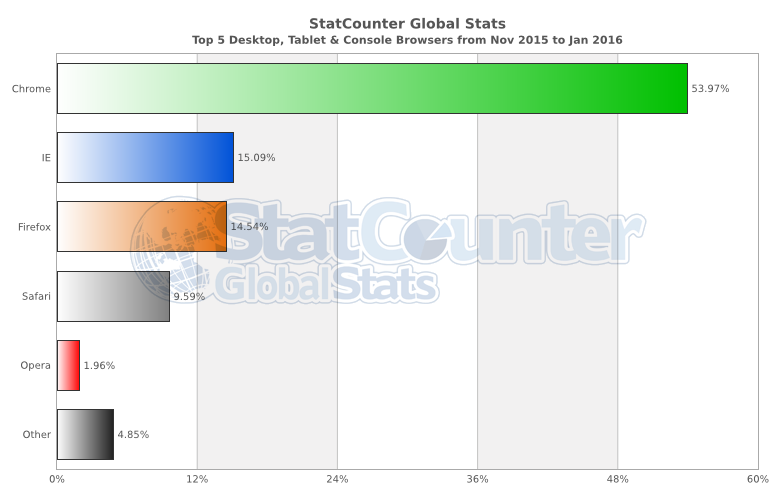
\includegraphics[height=5.5cm]{w_03_2016_Kharkevich2.png}
\caption*{StatCounter "--- статистика за 2015 год}
\end{figure}


\begin{figure}[h!]
  \centering
  
\includegraphics[width=10cm]{w_03_2016_Kharkevich3.png}
\caption*{Пример небезопаснго веб-сайта}\label{fig:Kharkevich3}
\end{figure}


При этом в Google уже с 2014 года предпочтение отдается сайтам с https\footnotemark[3].

\subsection*{Виды SSL-сертификатов}

Можно выделить следующие виды сертификатов:

\begin{itemize}
  \item Domain Validation "--- сертификат, подтверждающий только доменное имя.
  \item Organization Validation "--- сертификат, подтверждающий домен и организацию.
  \item Extended Validation "--- сертификат с расширенной проверкой.
\end{itemize}

Если Organization Validation и Extended Validation продаются только за деньги, то Domain Validation бывает и \textbf{бесплатный}.

В дальнейшем будем рассматривать только сертификаты Domain Validation.

\subsection*{Варианты получения SSL-сертификатов}

В реальной жизни для получения сертификатов существуют следующие варианты:

\begin{itemize}
  \item Самоподписанные сертификаты (self-signed-certificate) и сертификаты, подписанные собственным центром сертификации.
\begin{itemize}
  \item Из плюсов "--- возможность самостоятельно создавать \linebreak неограниченное количество SSL-сертификатов; отсутствие денежных затрат; быстрота в создании; в случае собственного удостоверяющего центра "--- доверие к данному сертификату.
  \item Из мнусов "--- необходимость добавления удостоверяющего центра в список доверенных ЦС вручную либо аналогичной процедуры для самоподписанных сертификатов; в случае использования собственного удостоверяющего центра "--- дополнительные требования по размещению и защите.
\end{itemize}


  \item Платные сертификаты от известных центров сертификации.
\begin{itemize}
  \item Из их плюсов "--- внешний гарант подлинности.
  \item Из минусов "--- нужно платить деньги.
\end{itemize}

  \item Коммерческие триальные SSL-сертификаты в качестве бесплатных.
\begin{itemize}
  \item Из их плюсов "--- бесплатность.
  \item Из минусов "--- малый срок действия и невозможность заказать повторно.
\end{itemize}

  \item Бесплатные сертификаты от StartSSL.
\begin{itemize}
  \item Из их плюсов "--- бесплатность.
  \item Из минусов "--- ручная установка сертификатов на сервер; сертификат бесплатен только для некоммерческого использования; сложности с отзывом сертификата.
\end{itemize}


  \item Бесплатные сертификаты от WoSign.
\begin{itemize}
  \item Из их плюсов "--- сертификат действительно бесплатный; у них появился англоязычный интерфейс; поддержка до пяти поддоменов в запросе на сертификат.

\begin{figure}[h!]
  \centering
  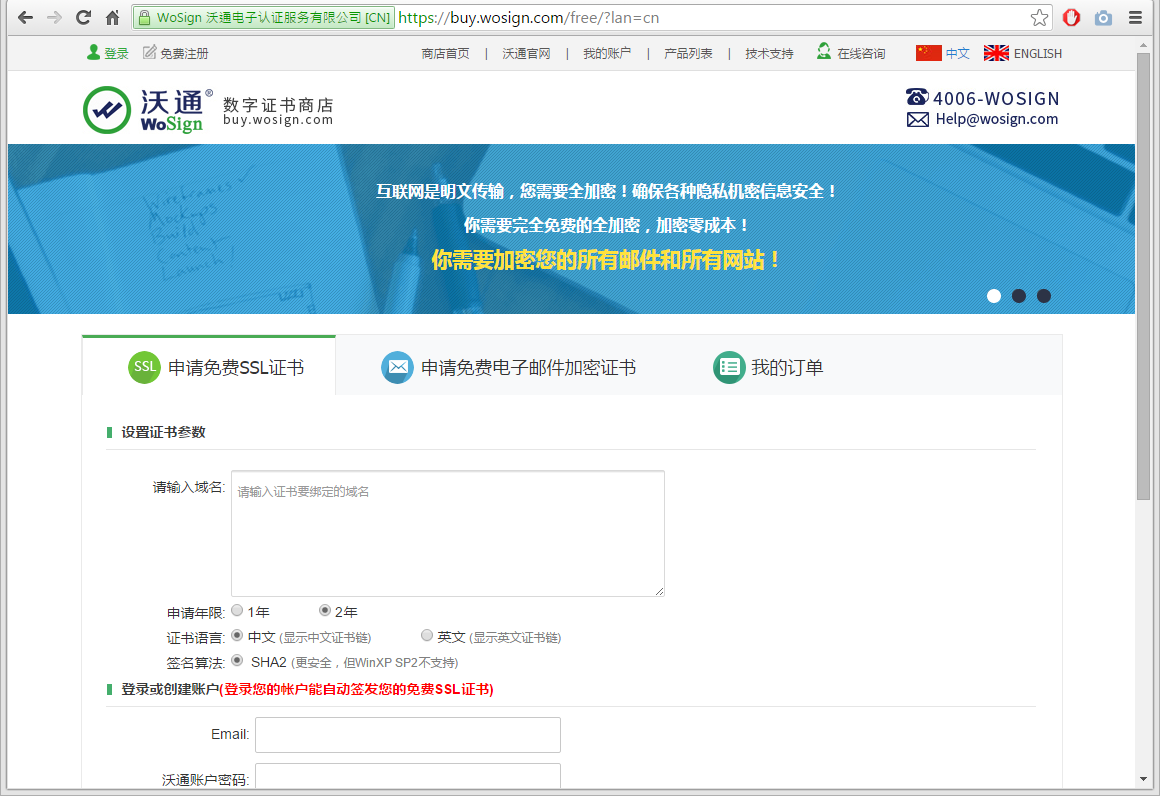
\includegraphics[height=5.5cm]{w_03_2016_Kharkevich4.png}
\caption*{WoSign на китайском языке}\label{fig:Kharkevich4}
\end{figure}

  \item Из минусов "--- ручная установка сертификатов на сервер; OCSP в Китае; для поддоменов постоянно урезаются лимиты; потенциальный MitM в связи с наличием \linebreak The Golden Shield Project.
\end{itemize}


  \item Бесплатные сертификаты от Let’s Encrypt.
\begin{itemize}
  \item Из минусов "--- новый игрок на рынке (требуется обновить списки CA); еще не вышел из бета-версии; только DV-сертификаты; есть некоторые лимиты на выпуск/перевыпуск сертификатов.
  \item Из плюсов "--- нет ограничения по применению сертификатов; может использоваться в коммерческих проектах; ACME "--- полностью автоматический процесс выдачи сертификата; срок действия сертификата до 90 дней.
\end{itemize}

\end{itemize}

\subsection*{Let’s Encrypt – наш выбор}
\begin{figure}[h!]
  \centering
  
\includegraphics[width=10cm]{w_03_2016_Kharkevich5.png}
  
\end{figure}

\subsubsection*{Шаги по установлению глобального доверия}

Для подписания пользовательских сертификатов Let’s Encrypt использует промежуточные сертификаты, которые кроме корневой подписи имеют перекрестную подпись от IdenTrust. Такая конфигурация позволила как минимум взлететь на тех браузерах, в которых еще ничего не было сказано про корневой сертификат Let’s Encrypt \footnotemark[4]

\begin{figure}[h!]
  \centering
  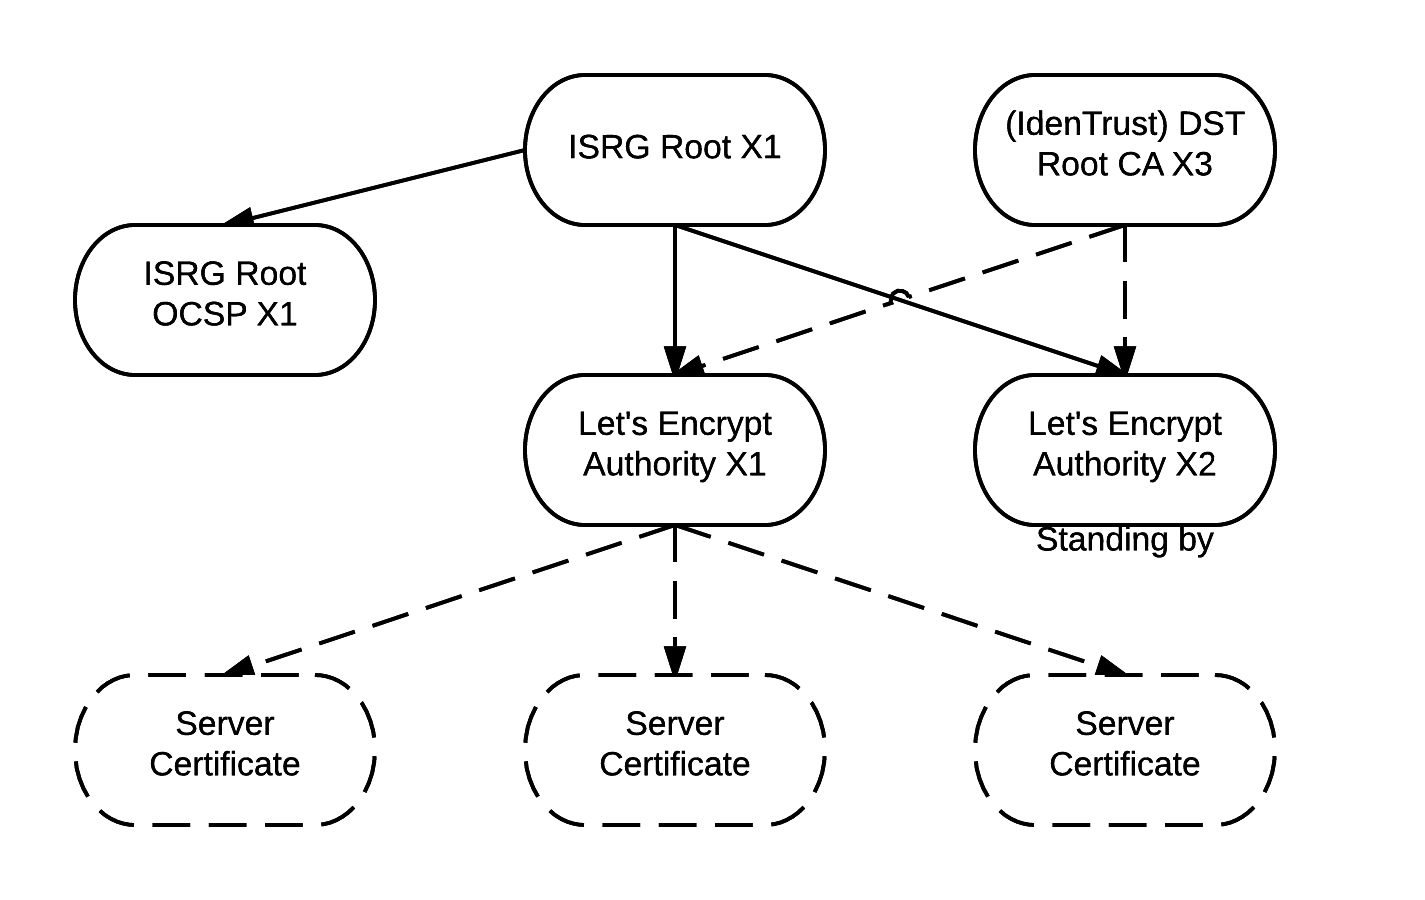
\includegraphics[height=5.5cm]{w_03_2016_Kharkevich6.png}
\caption*{Перекрестная подпись промежуточных сертификатов}\label{fig:Kharkevich6}
\end{figure}


\subsubsection*{Как работает ACME (Automatic Certificate Management Environment)}

Для получения  сертификата необходимо доказать центру сертификации, что домен, для которого пришел запрос сертификата, принадлежит запросившей сертификат стороне.

Это происходит в несколько шагов.

В первый раз взаимодействуя с Let's Encrypt CA, агент сгенерирует пару ключей, которые будет использовать для доказательства наличия прав на доменное имя.

Агент отправляет запрос в Let's Encrypt CA с указанием домена, который необходимо подтвердить.

Let’s Encrypt CA оценивает домен и выдает клиенту как минимум одну задачу на доказательство владения доменом:

\begin{itemize}
  \item Создание DNS-записи в доменной зоне для запрошенного домена.
  \item Создание ресурса, доступного по HTTP на известном URI для запрошенного домена.
\end{itemize}

Наряду с решением вышеописанной задачи, Let’s Encrypt CA  создает одноразовый ключ, который агент должен подписать своим закрытым ключом для домена, чтобы доказать, что он контролирует ключевую пару.

\begin{figure}[h!]
  \centering
  
\includegraphics[width=10cm]{w_03_2016_Kharkevich7.png}
  
\end{figure}

Агент выполняет выбранную задачу и уведомляет сервер о готовности пройти валидацию.

Let’s Encrypt CA проверяет электронную цифровую подпись и доступность файлов или записей в DNS.

В случае, если цифровая подпись верна и выбранная задача решена верно, Let’s Encrypt CA считает, что агент имеет право на управление сертификатами для запрошенного домена.

Ключевая пара, использованная агентом, становится <<авторизованной парой ключей>> для запрошенного домена.

\begin{figure}[h!]
  \centering
  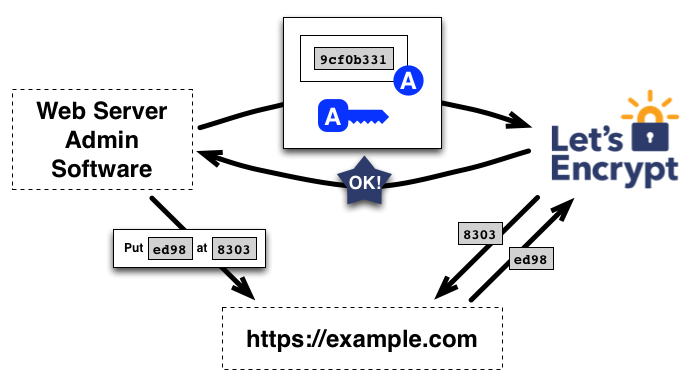
\includegraphics[height=5.5cm]{w_03_2016_Kharkevich8.png}
\caption*{Успешное выполнение всех задач от Let’s Encrypt}\label{fig:Kharkevich8}
\end{figure}


После авторизации агент может запросить, обновить или отозвать сертификаты для своего домена. Сообщения должны быть подписаны авторизованной парой ключей.

\begin{figure}[h!]
  \centering
  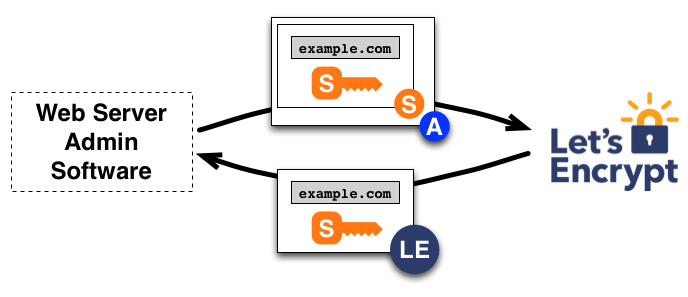
\includegraphics[width=10cm]{w_03_2016_Kharkevich9.png}
\caption*{Выпуск сертификата}\label{fig:Kharkevich9}
\end{figure}

\begin{figure}[h!]
  \centering
  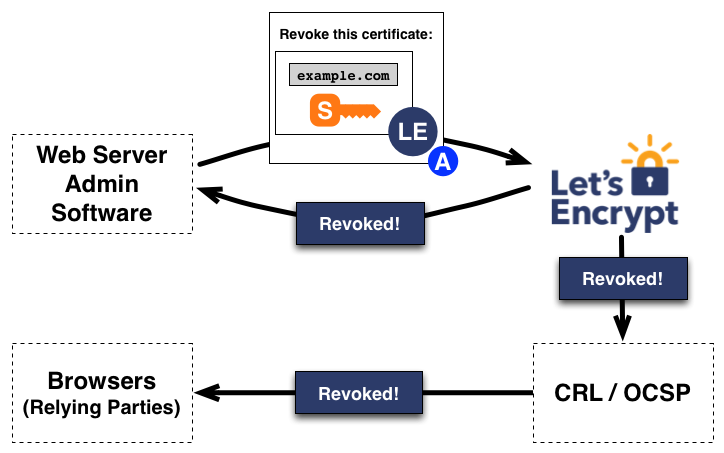
\includegraphics[height=5.5cm]{w_03_2016_Kharkevich10.png}
\caption*{Отзыв сертификата}\label{fig:Kharkevich10}
\end{figure}


\subsubsection*{Клиенты/плагины для Let's Encrypt}

Для Let’s Encrypt существует как официальная реализация клиентской части, так и множество других реализаций протокола \linebreak ACME (написаны на Python, Go, C\#, Ruby, Bash).

Официальный клиент поддерживает расширение функциональности за счет плагинов. На текущий момент, реализованные плагины представлены на странице github \footnotemark[5].

Написать свой плагин достаточно просто: нужно всег лишь прочитать документацию \footnotemark[6] и написать его.

\subsection*{Примеры из реальной жизни и немного статистики}

Судя по crt.sh "--- Let's Encrypt выпустил громадное количество сертификатов и с отрывом лидирует над остальными.

\begin{figure}[h!]
  \centering
  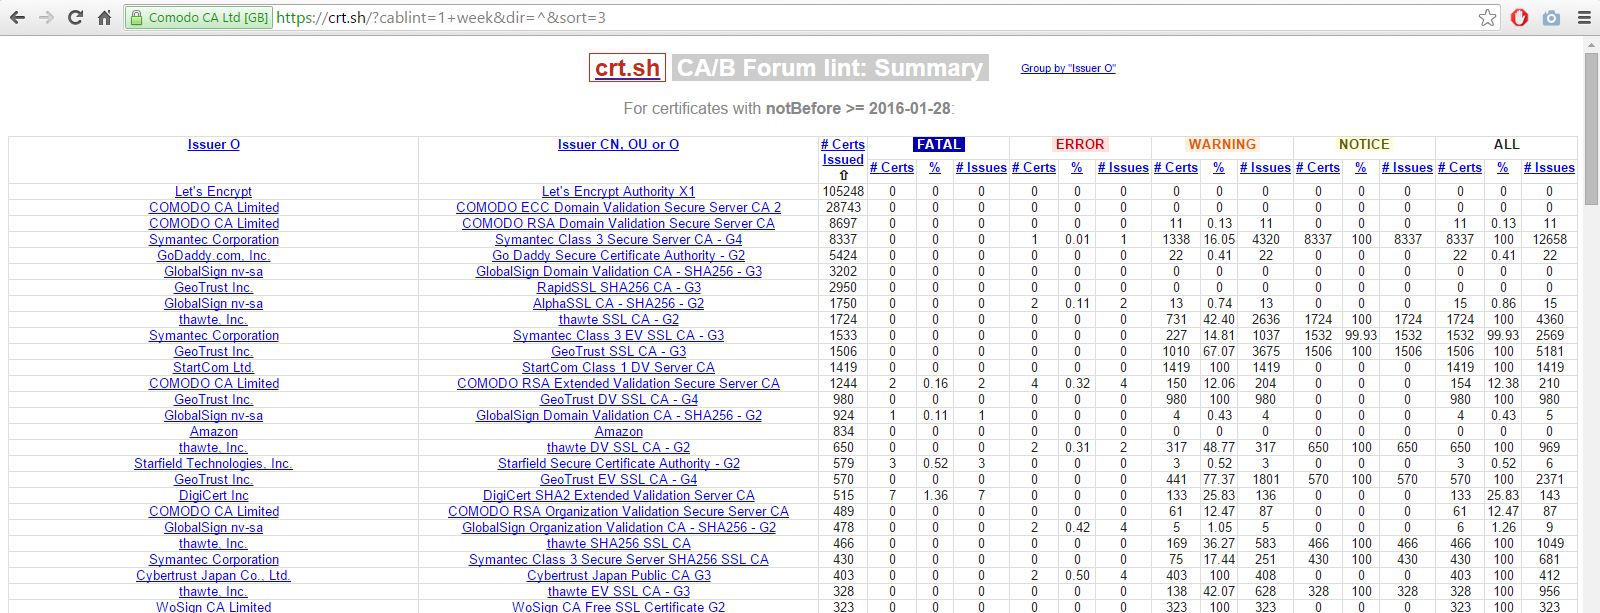
\includegraphics[width=10cm]{w_03_2016_Kharkevich11.png}
\caption*{Статистика по версии от crt.sh}\label{fig:Kharkevich11}
\end{figure}


\subsubsection*{Забытые обновления сертификатов}

В заключение "--- несколько случаев пропущенных обновлений сертификатов:

\begin{itemize}
  \item Ростелеком в 2010 году \footnotemark[7]
  \item Хабр и habrastorage.org в 2014 году \footnotemark[8]

\begin{figure}[h!]
  \centering
  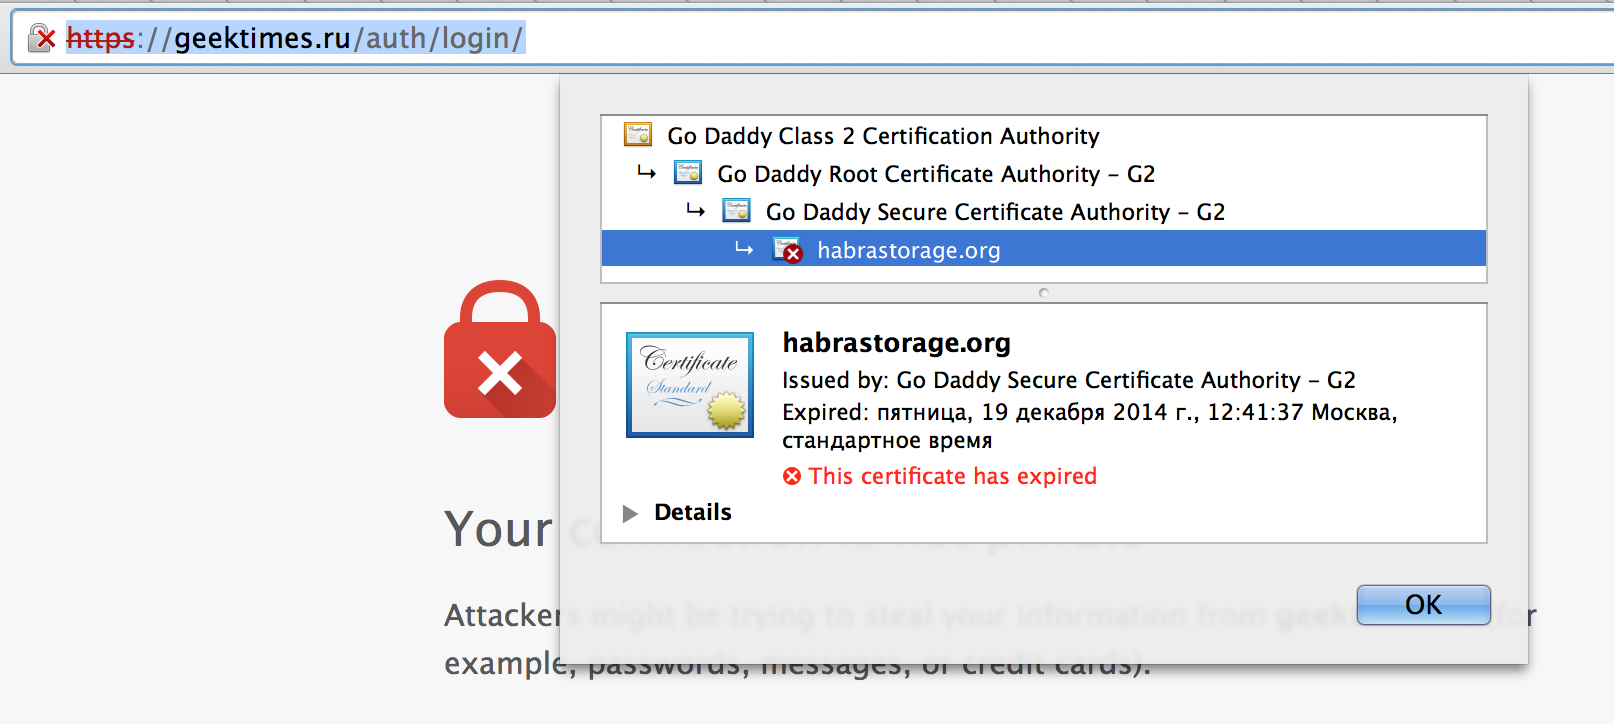
\includegraphics[width=10cm]{w_03_2016_Kharkevich12.png}
  
\end{figure}

  \item RU-CENTER (ssl.ru) в 2016 году

\begin{figure}[h!]
  \centering
  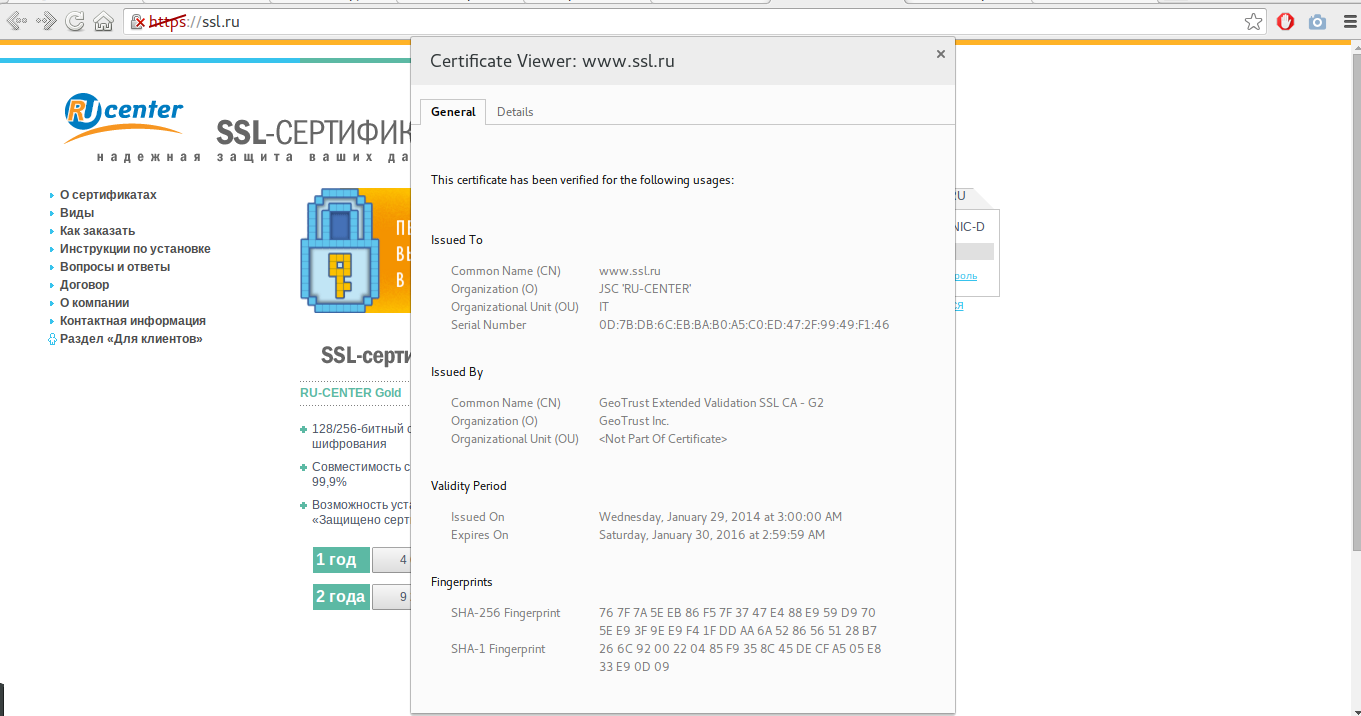
\includegraphics[height=5.5cm]{w_03_2016_Kharkevich13.png}
  
\end{figure}

\end{itemize}

\begin{thebibliography}{99}

\bibitem{Kharkevich1} \url{https://blog.mozilla.org/security/2015/04/30/deprecating-non-secure-http/} {Mozilla Security Blog: Deprecating Non-Secure HTTP}
\bibitem{Kharkevich2}\url{https://www.chromium.org/Home/chromium-security/marking-http-as-non-secure}{The Chromium Projects proposal: Marking HTTP As Non-Secure}
\bibitem{Kharkevich3}\url{https://googlewebmastercentral.blogspot.com.by/2014/08/https-as-ranking-signal.html}{Google Webmaster Central Blog: HTTPS as a ranking signal}
\bibitem{Kharkevich4}\url{https://letsencrypt.org/certificates/}{Let’s Encrypt certificates}
\bibitem{Kharkevich5}\url{https://github.com/letsencrypt/letsencrypt/wiki/Plugins}{Letsencrypt officially supported plugins}
\bibitem{Kharkevich6}\url{https://letsencrypt.readthedocs.org/en/latest/contributing.html#dev-plugin}{Writing your own letsencrypt plugin}
\bibitem{Kharkevich7}\url{https://geektimes.ru/post/102984/}{Geektimes: Ростелеком забыл обновить ssl-сертификат gosuslugi.ru}
\bibitem{Kharkevich8}\url{https://geektimes.ru/post/243231/}{Geektimes: Пора обновить сертификат на Habrastorage.org!}
\bibitem{Kharkevich9\url{https://crt.sh/}{Поиск по сертификатам}.
\bibitem{Kharkevich10}\url{https://www.ssllabs.com/ssltest/}{Тестирование конфигурации SSL}.
\bibitem{Kharkevich11}\url{https://mozilla.github.io/server-side-tls/ssl-config-generator/}{Генератор SSL конфигурационных файлов от Mozilla}.
\bibitem{Kharkevich12}\url{http://gs.statcounter.com/}{Анализ веб-трафика}.
\bibitem{Kharkevich13}\url{https://letsencrypt.org/howitworks/technology/}{Let's Encrypt how it works}.

\end{thebibliography}
\end{document}

\documentclass[10pt, a5paper]{article}
\usepackage{pdfpages}
\usepackage{parallel}
\usepackage[T2A]{fontenc}
\usepackage{ucs}
\usepackage[utf8x]{inputenc}
\usepackage[polish,english,russian]{babel}
\usepackage{hyperref}
\usepackage{rotating}
\usepackage[inner=2cm,top=1.8cm,outer=2cm,bottom=2.3cm,nohead]{geometry}
\usepackage{listings}
\usepackage{graphicx}
\usepackage{wrapfig}
\usepackage{longtable}
\usepackage{indentfirst}
\usepackage{array}
\newcolumntype{P}[1]{>{\raggedright\arraybackslash}p{#1}}
\frenchspacing
\usepackage{fixltx2e} %text sub- and superscripts
\usepackage{icomma} % коскі ў матэматычным рэжыме
\PreloadUnicodePage{4}

\newcommand{\longpage}{\enlargethispage{\baselineskip}}
\newcommand{\shortpage}{\enlargethispage{-\baselineskip}}

\def\switchlang#1{\expandafter\csname switchlang#1\endcsname}
\def\switchlangbe{
\let\saverefname=\refname%
\def\refname{Літаратура}%
\def\figurename{Іл.}%
}
\def\switchlangen{
\let\saverefname=\refname%
\def\refname{References}%
\def\figurename{Fig.}%
}
\def\switchlangru{
\let\saverefname=\refname%
\let\savefigurename=\figurename%
\def\refname{Литература}%
\def\figurename{Рис.}%
}

\hyphenation{admi-ni-stra-tive}
\hyphenation{ex-pe-ri-ence}
\hyphenation{fle-xi-bi-li-ty}
\hyphenation{Py-thon}
\hyphenation{ma-the-ma-ti-cal}
\hyphenation{re-ported}
\hyphenation{imp-le-menta-tions}
\hyphenation{pro-vides}
\hyphenation{en-gi-neering}
\hyphenation{com-pa-ti-bi-li-ty}
\hyphenation{im-pos-sible}
\hyphenation{desk-top}
\hyphenation{elec-tro-nic}
\hyphenation{com-pa-ny}
\hyphenation{de-ve-lop-ment}
\hyphenation{de-ve-loping}
\hyphenation{de-ve-lop}
\hyphenation{da-ta-ba-se}
\hyphenation{plat-forms}
\hyphenation{or-ga-ni-za-tion}
\hyphenation{pro-gramming}
\hyphenation{in-stru-ments}
\hyphenation{Li-nux}
\hyphenation{sour-ce}
\hyphenation{en-vi-ron-ment}
\hyphenation{Te-le-pathy}
\hyphenation{Li-nux-ov-ka}
\hyphenation{Open-BSD}
\hyphenation{Free-BSD}
\hyphenation{men-ti-on-ed}
\hyphenation{app-li-ca-tion}

\def\progref!#1!{\texttt{#1}}
\renewcommand{\arraystretch}{2} %Іначай формулы ў матрыцы зліпаюцца з лініямі
\usepackage{array}

\def\interview #1 (#2), #3, #4, #5\par{

\section[#1, #3, #4]{#1 -- #3, #4}
\def\qname{LVEE}
\def\aname{#1}
\def\q ##1\par{{\noindent \bf \qname: ##1 }\par}
\def\a{{\noindent \bf \aname: } \def\qname{L}\def\aname{#2}}
}

\def\interview* #1 (#2), #3, #4, #5\par{

\section*{#1\\{\small\rm #3, #4. #5}}

\def\qname{LVEE}
\def\aname{#1}
\def\q ##1\par{{\noindent \bf \qname: ##1 }\par}
\def\a{{\noindent \bf \aname: } \def\qname{L}\def\aname{#2}}
}

\switchlang{en}
\begin{document}
\title{Comparative Review of FLOSS Testing Frameworks for Embedded C++}
\author{Алексей Хлебников, Oslo, norway}
\maketitle
\begin{abstract}
Every software development group tests its products, yet delivered software always has defects. Test engineers strive to catch them before the product is released but they always creep in and they often reappear, even with the best manual testing processes. Automated tests is the best way to increase \linebreak the effectiveness, efficiency and coverage of your software testing. This comparative review evaluates several C++ testing \linebreak frameworks with focus on usage in modern embedded systems, like Android and iOS.
\end{abstract}
\subsection*{Requirements}

It turns out that most automated testing frameworks for C++ were designed for Desktop, as opposed to Embedded devices. They usually report test results to standard output, many frameworks even supply main() function. On Embedded platforms we usually don't have stdout and applications can not use main() function, generated by the frameworks. We need to capture testing report into memory and then either output it to the log, or to some nice window on the device.

Thus, our requirements for testing frameworks are as follows:

\begin{itemize}
  \item Cross-platform, i.e. support for testing on Android, iOS, Linux, MacOS X, Windows.
  \item Support for custom test runner, because we don't have main() on Android or iOS.
  \item Support for custom outputter, because we don't have stdout on Android and iOS.
  \item Support for fixtures, i.e. setup/teardown.
  \item Support for testsuites, i.e. test grouping.
\end{itemize}

Non-mandatory, but desired features:

\begin{itemize}
  \item Easy and pleasant to use: Sensible and logical design, good \linebreak documentation, sensible syntax, terminology and keywords.
  \item The framework should be supported and mature.
  \item The less boilerplating "--- the better. For example, automatic test registration.
  \item Support for running test selectively, preferably by regex match on test names.
  \item Support for listing available tests.
\end{itemize}

\subsection*{Testing framework list}

The following testing frameworks were evaluated:

\begin{itemize}
  \item Bandit
  \item Boost.Test
  \item CATCH
  \item CppUnit
  \item CxxTest
  \item Google Test
  \item Igloo
  \item Lest
  \item TUT
  \item UnitTest++
\end{itemize}

\subsection*{More about each framework}

\subsubsection*{CppUnit}

C++'s classics of the classics. The first xUnit-like testing framework for C++. Powerful and feature-rich. Has good documentation. \linebreak Unfortunately, test registration is not automatic and developer will need to retype test class and function names several times. xUnit-like frameworks in other languages, like Java and Ruby, do not require such manual test registration, because they, unlike C++, have reflection mechanisms, which are used for automatic test discovery.

Code example:
\begin{verbatim}
class MyTestSuite : public CppUnit::TestFixture
{
public:
    void setUp()
    {
        m_num = 2;
    }

    void tearDown()
    {
        m_num = 0;
    }

    void testOneThing()
    {
        CPPUNIT_ASSERT(m_num == 2);
    }

    void testAnotherThing()
    {
        CPPUNIT_ASSERT_EQUAL(m_num * m_num, 4);
    }
    ...
};

...

auto* suite = new CppUnit::TestSuite("MyTestSuite");

suite->addTest(
    new CppUnit::TestCaller <MyTestSuite> (
        "testOneThing",
        &MyTestSuite::testOneThing
    )
);

suite->addTest(
    new CppUnit::TestCaller <MyTestSuite> (
        "testAnotherThing",
        &MyTestSuite::testAnotherThing
    )
);

CppUnit::TextUi::TestRunner runner;

runner.addTest(suite);

\end{verbatim}

Supports:

\begin{itemize}
  \item Custom runner.
  \item Custom outputter by subclassing class TextOutputter and \linebreak overriding 1 function.
  \item Fixtures and testsuites.
  \item Listing available tests.
  \item Selective running of one particular test.
  \item Unlike most other frameworks, defining and registering test both using C++-only code and using macros.
\end{itemize}

Downsides:

\begin{itemize}
  \item Test autoregistration is almost non-existing. There are helper macros, but they do not help enough.
  \item This framework requires much boilerplating. People on the Internet complain about it a lot.
  \item The framework is supported, but not very actively. Currently it is supported by LibreOffice team. On the other hand, the framework already has so many features, that it does not need much further development. Sure, there is a room for improvement with boilerplating, but such work suggests so much refactoring that it is easier to just take another testing framework.
\end{itemize}

Verdict:

CppUnit requires too much boilerplating. It was probably OK 15 years ago, when C++ developers did not have much choice, but for 2016 it is too bad.

\subsubsection*{Google Test}

Powerful framework with lots of features and complicated syntax. Has good documentation. Unfortunately, it is hard to redirect output. It is one of the first testing frameworks, featuring automatic test \linebreak registration. C++ still does not have reflection, but Google Test \linebreak overcomes this obstacle by using macros, that both define and register tests.

Supports:

\begin{itemize}
  \item Custom runner.
  \item Fixtures and testsuites.
  \item Test autoregistration.
  \item Listing available tests.
  \item Running subset of tests, including and excluding them by path-like wildcards.
\end{itemize}

Downsides:

\begin{itemize}
  \item Custom outputter is not supported. The framework uses C file descriptors for output. The best that can be done is redirecting output to the file.
\end{itemize}

Verdict:

Google Test is not good enough for us, because custom outputter is not supported.

\subsubsection*{Boost.Test}

Powerful framework with lots of features and complicated syntax. Has good documentation. Did not support autoregistration before, but supports now. Can be compiled as static or dynamic library or used as header-only library. People on the Internet report that in case of header-only library compilation takes quite long time. Typical for a Boost library.

Code example:

\begin{verbatim}
struct MyFixtureStructure
{
    MyFixtureStructure()  { m_num = 2; }
    ~MyFixtureStructure() { m_num = 0; }
    ...
};

BOOST_FIXTURE_TEST_SUITE( MyTestSuite, MyFixtureStructure )

    BOOST_AUTO_TEST_CASE( test_one_thing )
    {
        BOOST_REQUIRE(m_num == 2);
    }

    BOOST_AUTO_TEST_CASE( test_another_thing )
    {
        BOOST_CHECK_EQUAL(m_num * m_num, 4);
    }

BOOST_AUTO_TEST_SUITE_END()

\end{verbatim}
Supports:

\begin{itemize}
  \item Custom runner.
  \item Custom outputter by subclassing std::ostream.
  \item Fixtures and testsuites.
  \item Test autoregistration.
  \item Listing available tests.
  \item Running subset of tests, selecting by path-like wildcards and tags.
\end{itemize}

Verdict:

Good candidate, supports all our requirements. Can we find better?

\subsubsection*{CxxTest}

Lightweight framework with good design and syntax. Implements automatic testcase registration by running a Python script, instead of clumsy macros, used by other testing frameworks. Each testsuite is a class with (optional) setUp/tearDown functions, each test is a function starting with <<test>>. As a result, a testsuite looks like a nice C++ class. The framework has good, even though not very long, documentation and easily readable source code otherwise.

Code example:

\begin{verbatim}
class MyTestSuite : public CxxTest::TestSuite
{
public:
    void setUp()
    {
        m_num = 2;
    }

    void tearDown()
    {
        m_num = 0;
    }

    void testOneThing()
    {
        TS_ASSERT(m_num == 2);
    }

    void testAnotherThing()
    {
        TS_ASSERT_EQUALS(m_num * m_num, 4);
    }
    ...
};
\end{verbatim}
Supports:

\begin{itemize}
  \item Custom runner.
  \item Custom outputter by subclassing class OutputStream and \linebreak overriding 3 functions.
  \item Fixtures and testsuites.
  \item Test autoregistration without macros.
  \item Listing available tests.
  \item Selective running of one particular test or testsuite.
\end{itemize}

Downsides:

\begin{itemize}
  \item Introduces dependency on Python for a C++ project.
  \item The Python script, used for testing code processing, has simplified C++ parser. Thus testing code must be kept parser-friendly. Fortunately, it is not hard.
\end{itemize}

Verdict:

Good candidate, supports all our requirements. Avoids macros, code looks cleaner. Can we still find better?

\subsubsection*{CATCH}

New-generation testing framework, supporting both usual xUnit-style tests and TDD/BDD-style tests with SECTIONS and \linebreak SCENARIOS. SECTIONS is a killer feature, allowing to save a lot of code on fixtures. SCENARIOS is development of the SECTIONS idea, more descriptive, but requires more typing.

Code example:

\begin{verbatim}
TEST_CASE( "My test suite name", "[my_tag]" )
{
    num = 2;

    SECTION( "increment" )
    {
        num++;
        REQUIRE(num == 3);
    }

    SECTION( "decrement" )
    {
        num--;

        SECTION( "increment after decrement" )
        {
            num++;
            REQUIRE(num == 2);
        }

        SECTION( "2 decrements" )
        {
            num--;
            REQUIRE(num == 0);
        }
    }
}
\end{verbatim}
Using SECTIONS, it is possible to combine fixture code with testing code. The above code is equivalent to 3 tests in xUnit model:

\begin{verbatim}
TEST_CASE( "increment" )
{
    num = 2;
    num++;
    REQUIRE(num == 3);
}

TEST_CASE( "increment after decrement" )
{
    num = 2;
    num--;
    num++;
    REQUIRE(num == 2);
}

TEST_CASE( "2 decrements" )
{
    num = 2;
    num--;
    num--;
    REQUIRE(num == 0);
}
\end{verbatim}
As we can see, SECTIONS provide a way to compactly describe several tests in a tree-like manner.

Supports:

\begin{itemize}
  \item Custom runner.
  \item Custom outputter by subclassing std::ostream.
  \item Fixtures and testsuites.
  \item SECTIONS and SCENARIOS!
  \item Test autoregistration.
  \item Listing available tests.
  \item Running subset of tests, selecting by path-like wildcards and tags.
\end{itemize}

Verdict:

Surprisingly good young contender. Supports all our requirements and in addition has SECTIONS killer feature. We have a winner!

Evaluation of other testing frameworks follows for completeness of the review.

\subsubsection*{Lest}

Aims to be C++11-fied version of CATCH. Seems to be less powerful than CATCH so far, and less mature. The first commit on GitHub for lest was in June 2013, vs November 2010 for CATCH. According to lest homepage, lest takes much more time to compile, probably because of excessive use of C++11 features.

\subsubsection*{Igloo}

BDD-style framework with unclear syntax and bad documentation. Seems to be inactively supported: the last commit on GitHub is from July 2015, but the last release was in 2013. Seems like the author devotes his attention to his another testing framework, Igloo.

\subsubsection*{Bandit}

Another BDD-style framework with unclear syntax and bad \linebreak documentation. C++11-fied version of Igloo framework from the same author. C++11 syntax was supposed to make the syntax better, but, I believe, the opposite happened: Bandit syntax is even worse than Igloo syntax, despite that the author calls it <<Human friendly unit testing for C++11>>.

\subsubsection*{TUT}

Old framework with awful syntax, relying on C++ templates instead of C++ macros. Unsupported: the last release was in 2013, commit rate is approximately 2 commits per year.

\subsubsection*{UnitTest++}

Minimalistic framework with <<usual>> syntax with C++ macros TEST/SUITE/CHECK/etc. Documentation is quite brief. \linebreak The framework seems to be supported, though not much development is being done, probably because the intention is to keep the framework minimalistic. The last release and the last commit was in November 2015.

Supports:

\begin{itemize}
  \item Custom runner.
  \item Custom outputter by subclassing class TestReporter and \linebreak overriding 4 functions.
  \item Fixtures and testsuites.
  \item Test autoregistration.
\end{itemize}

Downsides:

\begin{itemize}
  \item No support for listing available tests.
  \item No support for selective test running.
\end{itemize}

Verdict:

Good choice, if you want very light-weight and minimalistic \linebreak framework. If you want more features "--- choose something else.

\subsection*{Conclusion}

Considering upsides and downsides of different testing frameworks, I am giving top 3 places to these frameworks that satisfy all our \linebreak requirements:

\begin{enumerate}
  \item CATCH, for supporting SECTIONS.
  \item CxxTest, for avoiding clumsy macros, easy implementation of custom outputter and generally good design.
  \item Boost.Test, for being feature-rich, mature and quality product.
\end{enumerate}

\end{document}

\documentclass[10pt, a5paper]{article}
\usepackage{pdfpages}
\usepackage{parallel}
\usepackage[T2A]{fontenc}
\usepackage{ucs}
\usepackage[utf8x]{inputenc}
\usepackage[polish,english,russian]{babel}
\usepackage{hyperref}
\usepackage{rotating}
\usepackage[inner=2cm,top=1.8cm,outer=2cm,bottom=2.3cm,nohead]{geometry}
\usepackage{listings}
\usepackage{graphicx}
\usepackage{wrapfig}
\usepackage{longtable}
\usepackage{indentfirst}
\usepackage{array}
\newcolumntype{P}[1]{>{\raggedright\arraybackslash}p{#1}}
\frenchspacing
\usepackage{fixltx2e} %text sub- and superscripts
\usepackage{icomma} % коскі ў матэматычным рэжыме
\PreloadUnicodePage{4}

\newcommand{\longpage}{\enlargethispage{\baselineskip}}
\newcommand{\shortpage}{\enlargethispage{-\baselineskip}}

\def\switchlang#1{\expandafter\csname switchlang#1\endcsname}
\def\switchlangbe{
\let\saverefname=\refname%
\def\refname{Літаратура}%
\def\figurename{Іл.}%
}
\def\switchlangen{
\let\saverefname=\refname%
\def\refname{References}%
\def\figurename{Fig.}%
}
\def\switchlangru{
\let\saverefname=\refname%
\let\savefigurename=\figurename%
\def\refname{Литература}%
\def\figurename{Рис.}%
}

\hyphenation{admi-ni-stra-tive}
\hyphenation{ex-pe-ri-ence}
\hyphenation{fle-xi-bi-li-ty}
\hyphenation{Py-thon}
\hyphenation{ma-the-ma-ti-cal}
\hyphenation{re-ported}
\hyphenation{imp-le-menta-tions}
\hyphenation{pro-vides}
\hyphenation{en-gi-neering}
\hyphenation{com-pa-ti-bi-li-ty}
\hyphenation{im-pos-sible}
\hyphenation{desk-top}
\hyphenation{elec-tro-nic}
\hyphenation{com-pa-ny}
\hyphenation{de-ve-lop-ment}
\hyphenation{de-ve-loping}
\hyphenation{de-ve-lop}
\hyphenation{da-ta-ba-se}
\hyphenation{plat-forms}
\hyphenation{or-ga-ni-za-tion}
\hyphenation{pro-gramming}
\hyphenation{in-stru-ments}
\hyphenation{Li-nux}
\hyphenation{sour-ce}
\hyphenation{en-vi-ron-ment}
\hyphenation{Te-le-pathy}
\hyphenation{Li-nux-ov-ka}
\hyphenation{Open-BSD}
\hyphenation{Free-BSD}
\hyphenation{men-ti-on-ed}
\hyphenation{app-li-ca-tion}

\def\progref!#1!{\texttt{#1}}
\renewcommand{\arraystretch}{2} %Іначай формулы ў матрыцы зліпаюцца з лініямі
\usepackage{array}

\def\interview #1 (#2), #3, #4, #5\par{

\section[#1, #3, #4]{#1 -- #3, #4}
\def\qname{LVEE}
\def\aname{#1}
\def\q ##1\par{{\noindent \bf \qname: ##1 }\par}
\def\a{{\noindent \bf \aname: } \def\qname{L}\def\aname{#2}}
}

\def\interview* #1 (#2), #3, #4, #5\par{

\section*{#1\\{\small\rm #3, #4. #5}}

\def\qname{LVEE}
\def\aname{#1}
\def\q ##1\par{{\noindent \bf \qname: ##1 }\par}
\def\a{{\noindent \bf \aname: } \def\qname{L}\def\aname{#2}}
}

\begin{document}
\title{OpenBSD изнутри}
\author{Vadim Zhukov, Svetlana Savina, Moscow, Russia}
\maketitle
\begin{abstract}
The article would bring some light to the dark side of OpenBSD development process. You will know better: 1) about OpenBSD developers hierarchy; 2) what formal and informal rules are used in development process; 3) how OpenBSD development is sponsored nowadays; 4) what OpenBSD team building events AKA hackathons do look like; 5) how Ted Unangst became a verb; 6) and, finally, why do OpenBSD developers hate Australia.
\end{abstract}
Проект OpenBSD отличается от многих других проектов, занимающихся разработкой операционных систем. Здесь нет демократии, ни <<по западному>>, ни по какому-либо ещё типу. Не существует ни одной организации, которая могла бы с полным правом заявить, что контролирует проект, полностью или частично. Даже OpenBSD Foundation, будучи основанным несколькими членами сообщества, формально дистанцирован от проекта. Во многом такое положение дел является результатом основателя и главного дирижёра проекта "--- Тео де Раадта, человека крайне принципиального.

Разработку в OpenBSD можно условно разделить на две части: базовая система (включая xenocara, адаптированная для OpenBSD сборка X Window System) и порты. Разделение это во многом связано с разницей в объёмах и темпах обновления <<обслуживаемого>> исходного текста: в то время как базовая система насчитывает порядка 25 миллионов строк кода, в портах счёт идёт на сотни миллионов. При этом скорость выхода релизов у многих портов заметно больше, чем у OpenBSD; особенно это заметно на портах, находящихся на острие web-технологий: Web-движки и построенные на их базе браузеры. Как результат, имеются две основные чат-комнаты: <<для всех>> и, отдельная, для работающих над портами. Как правило, вторые редко пишут в первой, и наоборот.

В чатах общаются практически исключительно разработчики, посторонних там нет. Это не от стремления скрыть что-то важное и страшное от мира, а, скорее, наоборот: в чатах общение часто весьма неформальное, часто идёт обмен довольно личной информацией, выносить которую в списки рассылки не хочется.

О списках рассылки. Их на данный момент можно пересчитать по пальцам одной руки:
\begin{itemize}
  \item tech@ "--- для технических обсуждений: как правило, именно здесь предлагаются патчи и происходит их ревью.

  \item misc@ "--- для обсуждения всего подряд, включая жалобы на баги.

  \item announce@ "--- важные анонсы происходят через этот адрес.

  \item а также список рассылка под кодовым названием <<h>>, предназначенный для внутреннего пользования; причины закрытости те же, что и выше. Впрочем, иногда на нём также происходит ревью патчей, когда оным требуется особое внимание: письма с этого списка рассылки считаются наиболее приоритетными.
\end{itemize}

Существует также несколько узкоспециализированных, зачастую временных, ящиков для общения отдельных небольших команд <<по интересам>>. Часть из них "--- публичные, часть "--- нет.

Сам процесс разработки подразумевает ревью практически всего вносимого кода. Если попытаться формализовать список исключений, он окажется составлен примерно таким образом:

\begin{itemize}
  \item Обновление портов, производимое его мейнтейнером, или по его просьбе.

  \item Внесение изменений в userland-код их (со-)автором.

  \item Внесение изменений в ещё не стабилизированный, недавно внесённый код, производимое его (со-)автором до подключения данного кода в сборку.
\end{itemize}

Довольно часто как в базовой системе, так и в портах производится массовый неглубокий рефакторинг. В таком случае изменения обязательно тестируются кем-либо ещё, после чего и даётся <<okay>>. Согласия по каждому порту или каждой составляющей базовой системы при этом никто не спрашивает. Для внесения изменений в ядро и критичные системы обычно требуется минимум два <<okay>>; исключение составляют малофункциональные коммиты вроде добавления идентификаторов оборудования в таблицы PCI- и USB-устройств.

Стоит отметить, что web-сайт OpenBSD практически полностью находится в CVS-репозитории, а изменения обычно не требуют <<okay>>.

Как показывает опыт, в ходе разработки намного больше шансов имеет получить коммит, больше удаляющий, чем добавляющий.

В общем-то, это почти все правила. В целом процесс разработки больше завязан на людях, чем на правилах. Отчасти странно, что сообщество на редкость доброжелательных и полных энтузиазма людей заслужило славу агрессивно-враждебного. По всей видимости, виной тому сравнительно высокий уровень требований к желающим стать частью сообщества: чтобы стать разработчиком нужно <<всего лишь>> замучать разработчиков достаточно качественной работой, чтобы проще оказалось дать права на коммит, чем самому заниматься интеграцией.

Попасть в число разработчиков OpenBSD можно только по приглашению. Сначала приглашают пообщаться, и, если не поступает заметных возражений, приглашающий радует приглашённого предложением пообщаться с Тео. После этого обычно следует также приглашение посетить один из ближайших хакатонов.

Хакатоны "--- важная составляющая процесса разработки. В год проходит несколько хакатонов, в разных уголках света: это не только возможность встретиться и вживую решить многие накопившиеся вопросы, но ещё и познакомиться с другой страной и другими людьми. В частности, ежегодно проходит большой хакатон, где стараются собраться все разработчики (несколько десятков). В последние годы место большого хакатона стараются по разные стороны Атлантики: чётные в Европе, нечётные "--- в Америке.

Традиционно хакатон проходит около недели. Организаторы берут на себя помещение и напитки. Размещение и отдельные работы, если требуется, в последние годы оплачивает OpenBSD Foundation. Билеты же участники покупают сами. Так как даты хакатонов планируются сильно заранее (порой чуть ли не за год), то достать сравнительно недорогие билеты при желании труда не составляет.

Помимо хакатонов, OpenBSD Foundation оплачивает счета, связанные с поддержкой инфраструктуры проекта, помогает приобретать оборудование отдельным разработчикам, а также в течение последних нескольких лет курирует проекты в рамках программы Google Summer of Code.

\end{document}

\documentclass[10pt, a5paper]{article}
\usepackage{pdfpages}
\usepackage{parallel}
\usepackage[T2A]{fontenc}
\usepackage{ucs}
\usepackage[utf8x]{inputenc}
\usepackage[polish,english,russian]{babel}
\usepackage{hyperref}
\usepackage{rotating}
\usepackage[inner=2cm,top=1.8cm,outer=2cm,bottom=2.3cm,nohead]{geometry}
\usepackage{listings}
\usepackage{graphicx}
\usepackage{wrapfig}
\usepackage{longtable}
\usepackage{indentfirst}
\usepackage{array}
\newcolumntype{P}[1]{>{\raggedright\arraybackslash}p{#1}}
\frenchspacing
\usepackage{fixltx2e} %text sub- and superscripts
\usepackage{icomma} % коскі ў матэматычным рэжыме
\PreloadUnicodePage{4}

\newcommand{\longpage}{\enlargethispage{\baselineskip}}
\newcommand{\shortpage}{\enlargethispage{-\baselineskip}}

\def\switchlang#1{\expandafter\csname switchlang#1\endcsname}
\def\switchlangbe{
\let\saverefname=\refname%
\def\refname{Літаратура}%
\def\figurename{Іл.}%
}
\def\switchlangen{
\let\saverefname=\refname%
\def\refname{References}%
\def\figurename{Fig.}%
}
\def\switchlangru{
\let\saverefname=\refname%
\let\savefigurename=\figurename%
\def\refname{Литература}%
\def\figurename{Рис.}%
}

\hyphenation{admi-ni-stra-tive}
\hyphenation{ex-pe-ri-ence}
\hyphenation{fle-xi-bi-li-ty}
\hyphenation{Py-thon}
\hyphenation{ma-the-ma-ti-cal}
\hyphenation{re-ported}
\hyphenation{imp-le-menta-tions}
\hyphenation{pro-vides}
\hyphenation{en-gi-neering}
\hyphenation{com-pa-ti-bi-li-ty}
\hyphenation{im-pos-sible}
\hyphenation{desk-top}
\hyphenation{elec-tro-nic}
\hyphenation{com-pa-ny}
\hyphenation{de-ve-lop-ment}
\hyphenation{de-ve-loping}
\hyphenation{de-ve-lop}
\hyphenation{da-ta-ba-se}
\hyphenation{plat-forms}
\hyphenation{or-ga-ni-za-tion}
\hyphenation{pro-gramming}
\hyphenation{in-stru-ments}
\hyphenation{Li-nux}
\hyphenation{sour-ce}
\hyphenation{en-vi-ron-ment}
\hyphenation{Te-le-pathy}
\hyphenation{Li-nux-ov-ka}
\hyphenation{Open-BSD}
\hyphenation{Free-BSD}
\hyphenation{men-ti-on-ed}
\hyphenation{app-li-ca-tion}

\def\progref!#1!{\texttt{#1}}
\renewcommand{\arraystretch}{2} %Іначай формулы ў матрыцы зліпаюцца з лініямі
\usepackage{array}

\def\interview #1 (#2), #3, #4, #5\par{

\section[#1, #3, #4]{#1 -- #3, #4}
\def\qname{LVEE}
\def\aname{#1}
\def\q ##1\par{{\noindent \bf \qname: ##1 }\par}
\def\a{{\noindent \bf \aname: } \def\qname{L}\def\aname{#2}}
}

\def\interview* #1 (#2), #3, #4, #5\par{

\section*{#1\\{\small\rm #3, #4. #5}}

\def\qname{LVEE}
\def\aname{#1}
\def\q ##1\par{{\noindent \bf \qname: ##1 }\par}
\def\a{{\noindent \bf \aname: } \def\qname{L}\def\aname{#2}}
}

\begin{document}
\title{OpenBSD 5.8 \& 5.9}
\author{Vadim Zhukov, Moscow, russia}
\maketitle
\begin{abstract}
At the time of LVEE Winter, the OpenBSD repositories will be in pre-release lock, so it's a perfect time to take a deep look at changes happened. In particular: a) pledge(2): simple tool for improving security of your own programs; b) cloud-ready OpenBSD: native OpenBSD hypervisor, Xen support, improvements in service management; c) new oldies: file(1), doas(1); d) UTF-8 support for everybody.
\end{abstract}

В последний и грядущий релизы OpenBSD (5.8 и 5.9, соответственно) вошло немало изменений. Не пытаясь перечислить их все, остановимся на самых любопытных и неоднозначных.

\subsection*{pledge(2)}

Новый защитный фреймворк. Изначально анонсирован как \linebreak tame(2). Идея ограничения системных вызовов, используемых приложением, не нова. В том же OpenBSD уже давно имеется systrace, а в наиболее популярном открытом ядре, Linux, имеется разработанный когда-то в АНБ SELinux (строго говоря, последний делает больший акцент на файловые дескрипторы, но всё же). Главное отличие pledge(2) "--- семантический подход.

В pledge(2) системные вызовы сгруппированы в соответствии с типовыми профилями их использования. Более того, контроль в отдельных случаях ведётся на уровне аргументов системных вызовов: например, область <<unix>> разрешает работу с сокетами, но только в домене AF\_UNIX (они же AF\_LOCAL). Попытка создать или подключиться к сокету, скажем, по IPv4 приведёт к немедленной, неконтролируемой смерти программы.

Вызывать pledge(2) можно несколько раз во время выполнения программы, постепенно уменьшая количество требуемых привилегий. Собственно, идея pledge(2) во многом опирается на двухэтапную организацию процесса работы программы: сначала инициализация (возможно, требующая расширенных прав), а после "--- основной рабочий цикл программы, в котором программа занимается в основном обработкой данных и, скажем, не открывает новые сокеты.

Такой подход, конечно, конфликтует с ПО, которое позволяет переконфигурировать себя в ходе работы и не использует при этом разделение привилегий (priviledge separation). Однако стоит отметить, что за счёт такой <<гибкости>> такое ПО одновременно становится куда более уязвимым.

На данный момент под контроль pledge(2) переведена большая часть базовой системы OpenBSD (порядка 90\% всех приложений). Также поддержка pledge(2) постепенно добавляется в стороннее ПО, например: p7zip, mutt, Chromium/Iridium\ldots{} Сверх того, для данного API уже реализованы обвязки под ряд языков программирования, от Python до Haskell.

\subsection*{Поддержка хост-режима виртуализации и поддержка Xen}

OpenBSD уже несколько лет является добротной платформой для облачной инфраструктуры, но только в качестве гостевой системы. Хост-режим до недавнего времени был доступен только на платформе sparc64.

По ряду причин Reyk Floeter сотоварищи решили реализовывать гипервизор самостоятельно. На данный момент он умеет грузить только OpenBSD, поддержку других ОС стоит ожидать после релиза 5.9. Гипервизор не планируется настолько же богатым по возможностям, как, скажем, у VMWare. Конфигурационный файл vmd(8) легко читаем и схож по синтаксису с другими разработками OpenBSD, вроде httpd(8).

Параллельно с этим Михаил Белопухов реализовал поддержку паравиртуализации Xen. Благодаря проделанной Михаилом работе OpenBSD теперь может полноценно взаимодействовать с Xen-хостом, включая корректную инициализацию виртуальных \linebreak устройств.

Для поддержки различных гипервизоров ещё в OpenBSD 5.8 была добавлена специальная шина драйверов, pvbus(4). На данный момент она обеспечивает поддержку следующих гипервизоров: Hyper-V, KVM, VMware, Xen, а также, конечно, вышеупомянутого родного гипервизора.

\subsection*{file(1) и doas(1)}

Два сравнительно небольших изменения, отлично иллюстрирующих вектор развития OpenBSD.

\begin{itemize}
  \item file(1) и связанная с ней libmagic используются довольно часто. При этом в описании форматов, равно как и в самом коде file(1), нередко находят ошибки, уже не раз приводившие к опасным уязвимостям. При этом самой утилите, несмотря на сложную внутренню логику, практически не требуется какой-либо доступ к окружающей системе, а фактически используемый набор функций и запрашиваемых сведений о файлах весьма мал\ldots{} В итоге file(1) была переписана Nicholas Marriott (к слову, автором tmux) с использованием техники разделения привилегий: фактический разбор входного потока происходит в предельно ограниченном процессе, который от получает от мастер-процесса файловые дескрипторы для анализа.

  \item doas(1) "--- по сути, сильно упрощённая альтернатива sudo(8) с чуть более удобным синтаксисом. Общий код умещается в 822 строчки, включая комментарии и заголовочный файл. Для сравнения, в sudo 1.8.15 содержится 83596 строк. Из заметных <<потерь>> "--- sudoedit и явный проброс переменных окружения в командной строке.
\end{itemize}

\subsection*{UTF-8 для всех и каждого}

Свершилось то, чего давно ждали: OpenBSD уходит от однобайтных кодировок в сторону UTF-8. Хотя принято считать, что данный переход прозрачен, на самом деле существует целая россыпь подводных камней, прежде всего, в работе с терминальными приложениями: начиная от расчёта ширины строки и заканчивая, как ни удивительно, вопросами безопасности: если программа пытается честно, но не слишком внимательно, интерпретировать UTF-8, то злонамеренный пользователь может заставить её исказить обрабатываемые данные, или их отображение для других пользователей.

\begin{thebibliography}{99}
  \bibitem{Zhukov1} Презентация pledge. \url{http://www.openbsd.org/papers/hackfest2015-pledge/mgp00001.html}{}
  \bibitem{Zhukov2} Отчёт о хакатоне n2k15, включая рассказ о vmd. \url{http://undeadly.org/cgi?action=article&sid=20151217134417}{}
  \bibitem{Zhukov3} Анонс поддержки Xen. \url{http://undeadly.org/cgi?action=article&sid=20160114113445}{}
\end{thebibliography}

\end{document}

\documentclass[10pt, a5paper]{article}
\usepackage{pdfpages}
\usepackage{parallel}
\usepackage[T2A]{fontenc}
\usepackage{ucs}
\usepackage[utf8x]{inputenc}
\usepackage[polish,english,russian]{babel}
\usepackage{hyperref}
\usepackage{rotating}
\usepackage[inner=2cm,top=1.8cm,outer=2cm,bottom=2.3cm,nohead]{geometry}
\usepackage{listings}
\usepackage{graphicx}
\usepackage{wrapfig}
\usepackage{longtable}
\usepackage{indentfirst}
\usepackage{array}
\newcolumntype{P}[1]{>{\raggedright\arraybackslash}p{#1}}
\frenchspacing
\usepackage{fixltx2e} %text sub- and superscripts
\usepackage{icomma} % коскі ў матэматычным рэжыме
\PreloadUnicodePage{4}

\newcommand{\longpage}{\enlargethispage{\baselineskip}}
\newcommand{\shortpage}{\enlargethispage{-\baselineskip}}

\def\switchlang#1{\expandafter\csname switchlang#1\endcsname}
\def\switchlangbe{
\let\saverefname=\refname%
\def\refname{Літаратура}%
\def\figurename{Іл.}%
}
\def\switchlangen{
\let\saverefname=\refname%
\def\refname{References}%
\def\figurename{Fig.}%
}
\def\switchlangru{
\let\saverefname=\refname%
\let\savefigurename=\figurename%
\def\refname{Литература}%
\def\figurename{Рис.}%
}

\hyphenation{admi-ni-stra-tive}
\hyphenation{ex-pe-ri-ence}
\hyphenation{fle-xi-bi-li-ty}
\hyphenation{Py-thon}
\hyphenation{ma-the-ma-ti-cal}
\hyphenation{re-ported}
\hyphenation{imp-le-menta-tions}
\hyphenation{pro-vides}
\hyphenation{en-gi-neering}
\hyphenation{com-pa-ti-bi-li-ty}
\hyphenation{im-pos-sible}
\hyphenation{desk-top}
\hyphenation{elec-tro-nic}
\hyphenation{com-pa-ny}
\hyphenation{de-ve-lop-ment}
\hyphenation{de-ve-loping}
\hyphenation{de-ve-lop}
\hyphenation{da-ta-ba-se}
\hyphenation{plat-forms}
\hyphenation{or-ga-ni-za-tion}
\hyphenation{pro-gramming}
\hyphenation{in-stru-ments}
\hyphenation{Li-nux}
\hyphenation{sour-ce}
\hyphenation{en-vi-ron-ment}
\hyphenation{Te-le-pathy}
\hyphenation{Li-nux-ov-ka}
\hyphenation{Open-BSD}
\hyphenation{Free-BSD}
\hyphenation{men-ti-on-ed}
\hyphenation{app-li-ca-tion}

\def\progref!#1!{\texttt{#1}}
\renewcommand{\arraystretch}{2} %Іначай формулы ў матрыцы зліпаюцца з лініямі
\usepackage{array}

\def\interview #1 (#2), #3, #4, #5\par{

\section[#1, #3, #4]{#1 -- #3, #4}
\def\qname{LVEE}
\def\aname{#1}
\def\q ##1\par{{\noindent \bf \qname: ##1 }\par}
\def\a{{\noindent \bf \aname: } \def\qname{L}\def\aname{#2}}
}

\def\interview* #1 (#2), #3, #4, #5\par{

\section*{#1\\{\small\rm #3, #4. #5}}

\def\qname{LVEE}
\def\aname{#1}
\def\q ##1\par{{\noindent \bf \qname: ##1 }\par}
\def\a{{\noindent \bf \aname: } \def\qname{L}\def\aname{#2}}
}

\switchlang{en}
\begin{document}
\title{Yocto and OpenEmbedded at Collabora}
\author{Andrew Shadura, Bratislava, Slovakia}
\maketitle
\begin{abstract}
How the use of Yocto and OpenEmbedded helps corporations migrate to free software
\end{abstract}

There's a certain confusion existing even among people closely \linebreak working with Yocto Project, on what exactly Yocto is. First of all, Yocto isn't a Linux distribution. In fact, Yocto Project is an umbrella organisation that takes care of a bunch of embedded Linux technologies, including OpenEmbedded Core, BitBake, Poky and others. These and others technologies Yocto Project provides allow users to build custom Linux distributions suited to their own needs.

One might ask, if Yocto isn't a distribution, how does one make a distribution using its technologies?

\begin{figure}[h!]
  \centering
  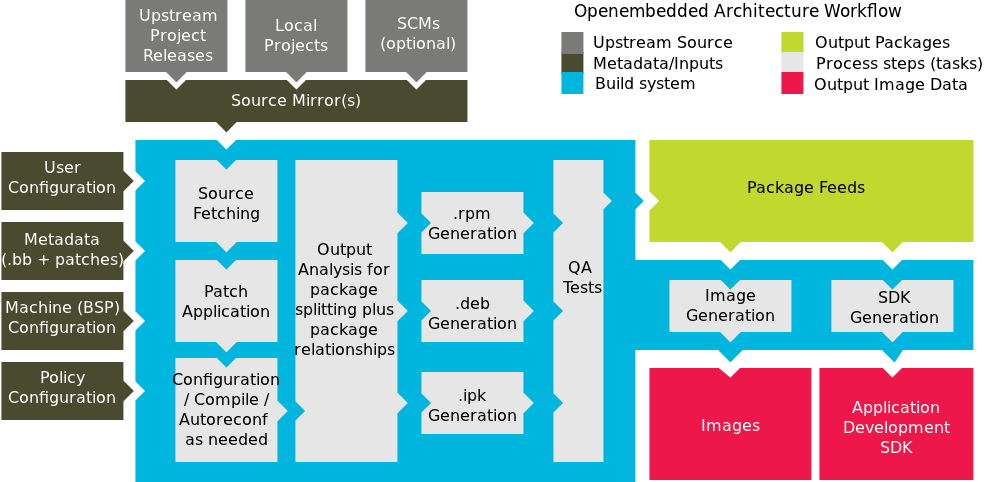
\includegraphics[height=4.5cm]{w_07_2016_Shadura1.png}
\end{figure}

The current Yocto technology stack has evolved from its roots in previously separate OpenEmbedded Project. Since the merger \linebreak of OpenEmbedded and Yocto, OpenEmbedded has introduced a layers system allowing vendors and users to have their bits separate yet \linebreak plugging into each other. There's a number of layers Yocto Project provides ({\ttfamily oe-core, meta-yocto, meta-yocto-bsp}) which form so-called \linebreak <<reference distribution>>, Poky. Poky contains foundation package \linebreak recipes (from OpenEmbedded Core), distribution policy\linebreak configuration, reference BSPs, build tools and documentation. Normally, Poky is what you start from when creating your own distribution.

\begin{figure}[h!]
  \centering
  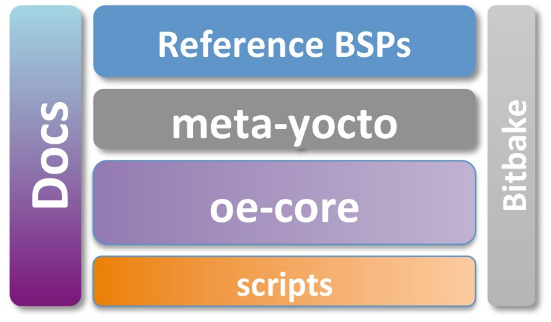
\includegraphics[height=2cm]{w_07_2016_Shadura2.png}
\end{figure}

Package recipes are written in a language similar to both Make and shell, and to certain extent resemble Gentoo's ebuilds. These recipes are being used by BitBake to build binary packages, and provide necessary information on where sources are found, and how to build them. BitBake recipes support includes, inheritance and overrides making it easy to change or extend the behaviour of an existing recipe without touching its code.

Fig: Example of a BitBake recipe:
\lstset{ %
anguage=C,                 % выбор языка для подсветки (здесь это С)
basicstyle=\small\sffamily, % размер и начертание шрифта для подсветки кода
breaklines=true,           % автоматически переносить строки (да\нет)
breakatwhitespace=false, % переносить строки только если есть пробел
}

\begin{lstlisting}
SUMMARY = "The canonical example of init scripts"
SECTION = "base"
LICENSE = "GPLv2"
LIC_FILES_CHKSUM = "file://${WORKDIR}/COPYRIGHT;md5=349c872e0066155e1818b786938876a4"

SRC_URI = "file://skeleton \
           file://skeleton_test.c \
           file://COPYRIGHT \
           "

do_compile () {
           ${CC} ${WORKDIR}/skeleton_test.c -o ${WORKDIR}/skeleton-test
}

do_install () {
           install -d ${D}${sysconfdir}/init.d
           cat ${WORKDIR}/skeleton | \
             sed -e 's,/etc,${sysconfdir},g' \
                 -e 's,/usr/sbin,${sbindir},g' \ 
                 -e 's,/var,${localstatedir},g' \ 
                 -e 's,/usr/bin,${bindir},g' \ 
                 -e 's,/usr,${prefix},g' > ${D}${sysconfdir}/init.d/skeleton 
           chmod a+x ${D}${sysconfdir}/init.d/skeleton 

           install -d ${D}${sbindir} 
           install -m 0755 ${WORKDIR}/skeleton-test ${D}${sbindir}/
}

RDEPENDS_${PN} = "initscripts"
CONFFILES_${PN} += "${sysconfdir}/init.d/skeleton"
\end{lstlisting}

Fig: Example of a BitBake recipe with inheritance:
\begin{lstlisting}
SUMMARY = "Example of how to build an external Linux kernel module"
LICENSE = "GPLv2"
LIC_FILES_CHKSUM = "file://COPYING;md5=12f884d2ae1ff87c09e5b7ccc2c4ca7e"

inherit module

SRC_URI = "file://Makefile \
           file://hello.c \
           file://COPYING \
          "

S = "${WORKDIR}"
\end{lstlisting}

Fig: Example of .bbappend:
\begin{lstlisting}
RDEPENDS_${PN}_append = " systemd"
\end{lstlisting}

Collabora is a company that provides consultancy to companies who are deploying open source technologies in their products, by providing its own open source based products and through knowledge sharing activities such as training. Collabora employs many free software \linebreak developers who are experts or major developers in such areas as \linebreak multimedia (GStreamer), graphics (Wayland, Weston), Linux kernel, productivity software (LibreOffice) and others.

At Collabora, we use Yocto on a project for a manufacturer of medical equipment, who use a Linux-based operating system in their products. Currently, their production devices are using a very custom Buildroot-based system, which runs quite an old (3.x-something) version of Linux kernel with lots of custom proprietary daemons and APIs. At some point they realised that it's quite a difficult task to support that system, and they decided they need help of experts, us.

For the project, the customer have decided to eliminate as much as possible custom proprietary libraries, take as much work as possible upstream, migrate to and integrate systemd as the init system. They also wanted us to help them with development methodology.

Thanks to the layer system Yocto Project uses, building your own distribution based on it is quite an easy job, once you know what you need from it. It all started as a layer with three files: the layer definition itself, distribution configuration file, and a machine definition.

Fig: Layer definition file (\verb!conf/layer.conf!)
\begin{lstlisting}
# We have a conf and classes directory, add to BBPATH
BBPATH .= ":${LAYERDIR}"

# We have recipes-* directories, add to BBFILES
BBFILES += "${LAYERDIR}/recipes-*/*/*.bb \
 ${LAYERDIR}/recipes-*/*/*.bbappend"
 
BBFILE_COLLECTIONS += "distro-core"
BBFILE_PATTERN_distro-core = "^${LAYERDIR}/"
BBFILE_PRIORITY_distro-core = "10"
\end{lstlisting}

Fig: Distribution definition file (\verb!conf/distro/badger.conf!)
\begin{lstlisting}
require conf/distro/poky.conf

DISTRO = "distro-core"
DISTRO_NAME = "Core Distro Platform"
DISTRO_VERSION = "2.0"
DISTRO_CODENAME = "badger"

DISTRO_FEATURES_append = " systemd wayland xwayland xattr pam apparmor"
DISTRO_FEATURES_remove = "x11"

# Enable systemd as init
VIRTUAL-RUNTIME_init_manager = "systemd"

# Disable sysv init and prevent any init scripts in the images
DISTRO_FEATURES_BACKFILL_CONSIDERED = "sysvinit"
VIRTUAL-RUNTIME_initscripts = ""

PREFERRED_PROVIDER_jpeg = "jpeg"
PREFERRED_PROVIDER_jpeg-native = "jpeg-native"
\end{lstlisting}

Fig: Machine definition file (\verb!conf/machine/vexpressa9.conf!)
\begin{lstlisting}
#@NAME: vexpress-a9 machine
#@DESCRIPTION: Machine configuration for the vexpress a9 board 

PREFERRED_PROVIDER_virtual/xserver = "xserver-xorg"

# Ship all kernel modules by default
MACHINE_EXTRA_RRECOMMENDS = " kernel-modules"

# Allow for MMC booting (required by the NAND-less)
EXTRA_IMAGEDEPENDS += ""

# Uncomment the following line to enable the hard floating point abi. Note that
# this breaks some binary libraries and 3D (neither of which ship with
# meta-yocto). For maximum compatibility, leave this disabled.
#DEFAULTTUNE ?= "cortexa8hf-neon"
include conf/machine/include/tune-cortexa9.inc

#IMAGE_CLASSES += "sdcard_image"

#IMAGE_FSTYPES += "tar.bz2 ext3 vexpressa9-sdimg"
IMAGE_FSTYPES += "tar.bz2 ext3"

#EXTRA_IMAGECMD_jffs2 = "-lnp "

# 2.6.37 and later kernels use OMAP_SERIAL, ttyO2
# earlier kernels use ttyS2
SERIAL_CONSOLE = "115200 ttyO2"

PREFERRED_PROVIDER_virtual/kernel ?= "linux-yocto"

KERNEL_IMAGETYPE = "zImage"
UBOOT_MACHINE = "ca9x4_ct_vxp_config"
UBOOT_ENTRYPOINT = "0x80008000"
UBOOT_LOADADDRESS = "0x80008000"
KERNEL_EXTRA_ARGS += "LOADADDR=${UBOOT_ENTRYPOINT}"

MACHINE_FEATURES = "kernel26 apm usbgadget usbhost vfat alsa"
\end{lstlisting}


These files define where recipe files are to be found, exactly what features (systemd, wayland, apparmor) we're using and what we don't (x11, sysvinit), and what processor architectures we're building for, what types of images we need to generate and so on.

For architecture-dependent parts, we first used a layer Freescale provided (meta-fsl-arm, meta-fsl-arm-extra), so we wouldn't need to write our own image generation routines, or tuning the cross-compiler features by hand. Later, we removed that dependency by bundling greatly simplified and customised versions of Freescale's recipes, but until we needed that it was a great help that we could reuse already working code.

When the initial phase of the project was completed, and we had a working image booting on a hardware prototype with Weston shell running, it was decided to split our layer in two, thus separating the platform itself and the application layer. Into the application layer went customer's proprietary software that will remain proprietary — at least, for now, and supporting daemons and libraries it depends on. The platform layer is almost entirely free software, with the exception of a few legacy hardware-related daemons which will be at some point replaced with their free software counterparts.

One might ask, why do we need anything in the platform layer apart from the distro configuration, if it's free software anyway? The answer is that, we're using quite some bleeding edge technology packages, but at the same time we want our platform to be based on the stable branch of Poky, the Yocto meta-distribution. That means, from time to time we need to import recipes for newer versions of software from the development branch. This is especially true when recipes coming from Yocto need to be improved: while BitBake allows extending existing recipes with use of .bbappend files, we mostly use that for distribution-specific things only. If we need some generic change that can be upstreamed, like user sessions support in systemd and dbus, we copy the latest version of the recipe from upstream, and patch it locally, so that the fixes can be easily submitted upstream.

This brings a benefit of needing minimal edits to the patches before they're submitted; otherwise we'd need a complete rewrite of the feature we need.

Apart from software updates and patches we also carry recipes for some free software which isn't release-ready, some custom configuration and some temporary workarounds for kernel bugs we don't currently have capacity to fix properly.

So far, since the project began, our team has contributed to the community at least the following:

\begin{itemize}
  \item lots of fixes to various OE Core package recipes, including patches enabling systemd integration, merged /usr
  \item patches to Weston and Linux kernel enabling accelerated graphics on our hardware
  \item patches to ifupdown adding inheritance feature similar to what BitBake has
  \item lot more
\end{itemize}

Kernel support for the customer's hardware is all being upstreamed by the customer, as the customer believes their hardware should run mainline kernel.

Even though the project is still in progress, even at its current stage it clearly demonstrates how is possible to migrate a big project to an open platform, reducing the maintenance cost and at the same time helping everyone else, and to a great extent that is possible thanks to Yocto.

\end{document}

\documentclass[10pt, a5paper]{article}
\usepackage{pdfpages}
\usepackage{parallel}
\usepackage[T2A]{fontenc}
\usepackage{ucs}
\usepackage[utf8x]{inputenc}
\usepackage[polish,english,russian]{babel}
\usepackage{hyperref}
\usepackage{rotating}
\usepackage[inner=2cm,top=1.8cm,outer=2cm,bottom=2.3cm,nohead]{geometry}
\usepackage{listings}
\usepackage{graphicx}
\usepackage{wrapfig}
\usepackage{longtable}
\usepackage{indentfirst}
\usepackage{array}
\newcolumntype{P}[1]{>{\raggedright\arraybackslash}p{#1}}
\frenchspacing
\usepackage{fixltx2e} %text sub- and superscripts
\usepackage{icomma} % коскі ў матэматычным рэжыме
\PreloadUnicodePage{4}

\newcommand{\longpage}{\enlargethispage{\baselineskip}}
\newcommand{\shortpage}{\enlargethispage{-\baselineskip}}

\def\switchlang#1{\expandafter\csname switchlang#1\endcsname}
\def\switchlangbe{
\let\saverefname=\refname%
\def\refname{Літаратура}%
\def\figurename{Іл.}%
}
\def\switchlangen{
\let\saverefname=\refname%
\def\refname{References}%
\def\figurename{Fig.}%
}
\def\switchlangru{
\let\saverefname=\refname%
\let\savefigurename=\figurename%
\def\refname{Литература}%
\def\figurename{Рис.}%
}

\hyphenation{admi-ni-stra-tive}
\hyphenation{ex-pe-ri-ence}
\hyphenation{fle-xi-bi-li-ty}
\hyphenation{Py-thon}
\hyphenation{ma-the-ma-ti-cal}
\hyphenation{re-ported}
\hyphenation{imp-le-menta-tions}
\hyphenation{pro-vides}
\hyphenation{en-gi-neering}
\hyphenation{com-pa-ti-bi-li-ty}
\hyphenation{im-pos-sible}
\hyphenation{desk-top}
\hyphenation{elec-tro-nic}
\hyphenation{com-pa-ny}
\hyphenation{de-ve-lop-ment}
\hyphenation{de-ve-loping}
\hyphenation{de-ve-lop}
\hyphenation{da-ta-ba-se}
\hyphenation{plat-forms}
\hyphenation{or-ga-ni-za-tion}
\hyphenation{pro-gramming}
\hyphenation{in-stru-ments}
\hyphenation{Li-nux}
\hyphenation{sour-ce}
\hyphenation{en-vi-ron-ment}
\hyphenation{Te-le-pathy}
\hyphenation{Li-nux-ov-ka}
\hyphenation{Open-BSD}
\hyphenation{Free-BSD}
\hyphenation{men-ti-on-ed}
\hyphenation{app-li-ca-tion}

\def\progref!#1!{\texttt{#1}}
\renewcommand{\arraystretch}{2} %Іначай формулы ў матрыцы зліпаюцца з лініямі
\usepackage{array}

\def\interview #1 (#2), #3, #4, #5\par{

\section[#1, #3, #4]{#1 -- #3, #4}
\def\qname{LVEE}
\def\aname{#1}
\def\q ##1\par{{\noindent \bf \qname: ##1 }\par}
\def\a{{\noindent \bf \aname: } \def\qname{L}\def\aname{#2}}
}

\def\interview* #1 (#2), #3, #4, #5\par{

\section*{#1\\{\small\rm #3, #4. #5}}

\def\qname{LVEE}
\def\aname{#1}
\def\q ##1\par{{\noindent \bf \qname: ##1 }\par}
\def\a{{\noindent \bf \aname: } \def\qname{L}\def\aname{#2}}
}

\switchlang{en}
\begin{document}
\title{An introduction to post-quantum cryptography}
\author{Andrew Savchenko, Moscow, Russia}
\maketitle
\begin{abstract}
These days cryptography faces a new type of threat: quantum
computing. An overview of quantum computing and how it works in the context of cryptography is presented. It is discussed when it is dangerous and when it is not for commonly used algorithms. There are well known, but not commonly used algorithms, which are resilient to the quantum computing approach and free \linebreak software is available to use them in a manner similar to GnuPG.
\end{abstract}
\subsection*{Preface}

Post-quantum cryptography is a way to preserve data security in the world of quantum computers: it is a set of algorithms and protocols resilient to cryptanalysis using quantum computing~\cite{Savchenko1}. It has nothing to do with quantum cryptography, which is a science of using quantum mechanical properties for cryptographic tasks (e.g. secure key \linebreak distribution based on quantum entanglement or data copy protection based on wave function collapse).

\subsection*{Quantum computing}

In classical electronics each bit can be in exactly one state: 0 or 1, e.g. byte of 8 bits can encode 256 states, but can be in only one state at once. Quantum bit (known as qubit) can also encode 0 or 1 state, but can be in superposition of both states at once, so 8 qubits describe 256 states simultaneously. Qubits can be operated by quantum gates the same way as bits are operated by microelectronics gates; quantum gates are very different in nature and properties from classical gates, but can also implement a full set of logical operations. The main power of quantum computing is that single quantum gate can operate on 2\^{}n states for n qubits available.

Quantum computers are probabilistic by the nature: 2+2 = 4 only sometimes, it may be 5 or -10 as well, but with different probabilities, so results must be verified or repeated many times to give acceptable error probability. Thus quantum computer is in no way replacement for classical computations, it is a dedicated machine that can augment classical computations, but never replace them.

\subsection*{Quantum algorithms}

There are many quantum algorithms available, but two of them are of the most importance for crypto analysis

\paragraph{Shor's algorithm}

Shor's algorithm~\cite{Savchenko2} allows for fast integer \linebreak factorization, thus breaking prime multiplication and elliptic curve \linebreak algorithms (RSA, ECDSA, ED25519 and so on). It is based on the idea of transforming factorization problem into function period finding problem (this is implemented using classical computing), finding period of a function using quantum Fourier transform. Then using a classical computations for continued fraction expansion prime can be obtained. Of course verification is needed.

As a result, search time is reduced from exponential to polynomial.

\paragraph{Grover's algorithm}

Grover's algorithm~\cite{Savchenko3} is a ``brute force'' algorithm which reduces search complexity from O(N) to O(sqrt(N)), thus halving key strength, e.g. AES-256 will be reduced to AES-128.

\subsection*{Impact on cryptographic algorithms.}

\begin{itemize}
  \item Symmetric key cryptography\begin{itemize}
  \item key strength is halved, this is a danger but solvable;
\end{itemize}


  \item Asymmetric key cryptography\begin{itemize}
  \item RSA/DSA/El-Gamal "--- dead;
  \item elliptic curves cryptography "--- dead;
  \item hash-based "--- halve reduced;
  \item code-based "--- halve reduced;
  \item lattice-based "--- halve reduced;
  \item and so on\ldots{}
\end{itemize}


\end{itemize}

There are plenty of asymmetric key algorithms which can't be \linebreak reduced to factorization problem. So why they are not used? The answer is: fast and effective implementation is also needed, but with modern CPUs it is not such a big problem.

\subsection*{Free software solutions}

\paragraph{Encryption}

Free software implementing algorithms resistible to \linebreak quantum computing exists! See codecrypt~\cite{Savchenko4} (LGPL-3). Main features:

\begin{itemize}
  \item functionality similar to GnuPG:\begin{itemize}
  \item key pair generation;
  \item signature;
  \item asymmetric encryption;
  \item symmetric encryption;
  \item import/export/recipients and so on
\end{itemize}


  \item many algorithms are implemented
\end{itemize}

Of course it is still new and don't rely on it blindly, better combine with GnuPG or other schemes.

Upstream is very dynamic and responsive!

\paragraph{Programming}

For those interested in quantum programming, you can try QCL~\cite{Savchenko5} (GPL-2): it is a quantum computing language with an emulator of a quantum computer!

\begin{thebibliography}{99}
\bibitem{Savchenko1}Daniel J. Bernstein, Johannes Buchmann, Erik Dahmen (editors). Post-quantum cryptography. Springer, Berlin, 2009. ISBN 978-3-540-88701-0. \url{https://pqcrypto.org/www.springer.com/cda/content/document/cda\_downloaddocument/9783540887010-c1.pdf}
\bibitem{Savchenko2}\url{https://en.wikipedia.org/wiki/Shor's\_algorithm}
\bibitem{Savchenko3}\url{https://en.wikipedia.org/wiki/Grover's\_algorithm}
\bibitem{Savchenko4}\url{http://e-x-a.org/codecrypt/}
\bibitem{Savchenko5}\url{http://tph.tuwien.ac.at/\~{}oemer/qcl.html}
\end{thebibliography}
\end{document}

\documentclass[10pt, a5paper]{article}
\usepackage{pdfpages}
\usepackage{parallel}
\usepackage[T2A]{fontenc}
\usepackage{ucs}
\usepackage[utf8x]{inputenc}
\usepackage[polish,english,russian]{babel}
\usepackage{hyperref}
\usepackage{rotating}
\usepackage[inner=2cm,top=1.8cm,outer=2cm,bottom=2.3cm,nohead]{geometry}
\usepackage{listings}
\usepackage{graphicx}
\usepackage{wrapfig}
\usepackage{longtable}
\usepackage{indentfirst}
\usepackage{array}
\newcolumntype{P}[1]{>{\raggedright\arraybackslash}p{#1}}
\frenchspacing
\usepackage{fixltx2e} %text sub- and superscripts
\usepackage{icomma} % коскі ў матэматычным рэжыме
\PreloadUnicodePage{4}

\newcommand{\longpage}{\enlargethispage{\baselineskip}}
\newcommand{\shortpage}{\enlargethispage{-\baselineskip}}

\def\switchlang#1{\expandafter\csname switchlang#1\endcsname}
\def\switchlangbe{
\let\saverefname=\refname%
\def\refname{Літаратура}%
\def\figurename{Іл.}%
}
\def\switchlangen{
\let\saverefname=\refname%
\def\refname{References}%
\def\figurename{Fig.}%
}
\def\switchlangru{
\let\saverefname=\refname%
\let\savefigurename=\figurename%
\def\refname{Литература}%
\def\figurename{Рис.}%
}

\hyphenation{admi-ni-stra-tive}
\hyphenation{ex-pe-ri-ence}
\hyphenation{fle-xi-bi-li-ty}
\hyphenation{Py-thon}
\hyphenation{ma-the-ma-ti-cal}
\hyphenation{re-ported}
\hyphenation{imp-le-menta-tions}
\hyphenation{pro-vides}
\hyphenation{en-gi-neering}
\hyphenation{com-pa-ti-bi-li-ty}
\hyphenation{im-pos-sible}
\hyphenation{desk-top}
\hyphenation{elec-tro-nic}
\hyphenation{com-pa-ny}
\hyphenation{de-ve-lop-ment}
\hyphenation{de-ve-loping}
\hyphenation{de-ve-lop}
\hyphenation{da-ta-ba-se}
\hyphenation{plat-forms}
\hyphenation{or-ga-ni-za-tion}
\hyphenation{pro-gramming}
\hyphenation{in-stru-ments}
\hyphenation{Li-nux}
\hyphenation{sour-ce}
\hyphenation{en-vi-ron-ment}
\hyphenation{Te-le-pathy}
\hyphenation{Li-nux-ov-ka}
\hyphenation{Open-BSD}
\hyphenation{Free-BSD}
\hyphenation{men-ti-on-ed}
\hyphenation{app-li-ca-tion}

\def\progref!#1!{\texttt{#1}}
\renewcommand{\arraystretch}{2} %Іначай формулы ў матрыцы зліпаюцца з лініямі
\usepackage{array}

\def\interview #1 (#2), #3, #4, #5\par{

\section[#1, #3, #4]{#1 -- #3, #4}
\def\qname{LVEE}
\def\aname{#1}
\def\q ##1\par{{\noindent \bf \qname: ##1 }\par}
\def\a{{\noindent \bf \aname: } \def\qname{L}\def\aname{#2}}
}

\def\interview* #1 (#2), #3, #4, #5\par{

\section*{#1\\{\small\rm #3, #4. #5}}

\def\qname{LVEE}
\def\aname{#1}
\def\q ##1\par{{\noindent \bf \qname: ##1 }\par}
\def\a{{\noindent \bf \aname: } \def\qname{L}\def\aname{#2}}
}

\begin{document}
\title{Создание робота для Roborace}
\author{Dmitry Sklipus, Brest, Belarus}
\maketitle
\begin{abstract}
Author shares his development experience of Arduino-based robots targeted at Roborace competitions. Specifics of the competition is explained as far as some details of the hardware platform and the contol algorythm.
\end{abstract}
\subsection*{Специфика Roborace}

Roborace "--- это состязания, в которых соревнуются \linebreak роботы-автомобили на специальной кольцевой трассе. Можно провести некоторую аналогию между Roborace и гонками Формулы 1, за исключением двух моментов.

\begin{itemize}
  \item Во-первых, вместо полномасштабных гоночных болидов участвуют уменьшенные модели авто и оригинальные конструкции с габаритными и весовыми ограничениями (максимальные ШхД=25х50 см и вес до 3 кг).
  \item Во-вторых, вместо пилотов автомобилем управляет бортовой компьютер, который анализирует показания различных датчиков и ориентирует автомобиль на трассе, выбирает скорость движения, предотвращает столкновения с препятствиями и соперниками. Собственно “поведение” авто на трассе определяется управляющей программой бортового компьютера.
\end{itemize}

Roborace проводится в виде чемпионата, состоящего из этапов, которые организуются в различных городах Беларуси и за рубежом. Участие в чемпионате принимают как конструкции начального уровня (например, на базе конструктора типа LEGO), так и сложные робототехнические устройства. Регламенты соревнований формируются таким образом, чтобы охватить как можно более широкий спектр характеристик и возможностей робототехнических конструкций.


\begin{figure}[h!]
  \centering
  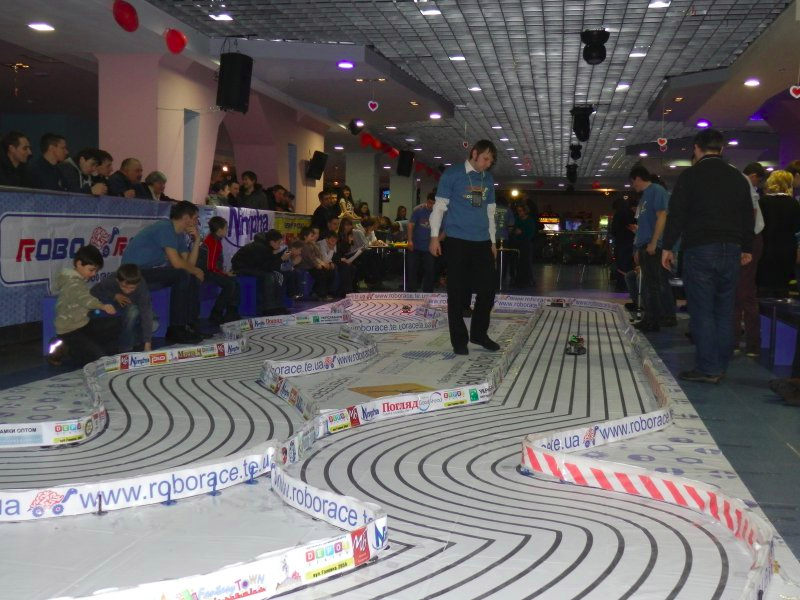
\includegraphics[width=10cm]{w_09_2016_Sklipus1.png}
  \caption {Трасса для гонок роботов}\label{Sklipus1}
\end{figure}

Рассмотрим трассу, изображенную на рисунке ~\ref{Sklipus1}, по которой предстоит перемещаться роботу. Обязательными элементами являются черные линии и стенки. Исходя из этого можно строить стратегию движения робота по трассе: например, оборудовать робота датчиками черной линии и использовать линии трассы для навигации, или установить дальномеры для обнаружения препятствий и двигаться вдоль стенок.

В рамках данной статьи представлен один из роботов, разработанный мной для Roborace по второй стратегия (движение на основе показаний дальномеров).

\subsection*{Этапы создания робота}

Создание робота для Roborace начинается с выбора шасси. Сейчас магазины предлагают большой выбор гусеничных и колесных платформ. Я рекомендую остановиться на классической схеме, когда задние колеса приводятся в движение электродвигателем, а передние управляются сервоприводом~\cite{Sklipus1}. На рисунке ~\ref{Sklipus2} изображен робот для Roborace, построенный по подобной схеме.

\begin{figure}[h!]
  \centering
  \includegraphics[width=10cm]{w_09_2016_Sklipus2.png}
  \caption {Робот}\label{Sklipus2}
\end{figure}

Мне повезло за небольшие деньги приобрести модель в местном клубе радио-моделистов (читатели могут попытаться сделать то же самое в своем регионе: обычно у них много устаревших моделей). Так как в приобретенной модели не было тягового электродвигателя, на нее был установлен установил купленный 12-вольтный мотор. Можно было также использовать обычную игрушку: они обычно довольно живучи, и требуется только модифицировать рулевое управление.

Так как в моем случае сервопривод уже был установлен, с ним проблем не возникло.

Следующий этап "--- выбор платы управления. Тут есть множество вариантов. Я выбрал Arduino как самый простой вариант. То же можно порекомендовать и читателю, особенно при недостатке опыта. Исходя из моего достаточно большого опыта, для таких роботов достаточно обычных 8-битных микроконтроллеров. Поэтому если не планируется использовать для отслеживания движений робота камеру, не стоит усложнять его более мощным процессором.

Сервопривод можно напрямую подключить к Arduino "--- например, через sensor shield, изображенный на рисунке ~\ref{Sklipus3}. К нему также удобно подключать датчики.

\begin{figure}[h!]
  \centering
  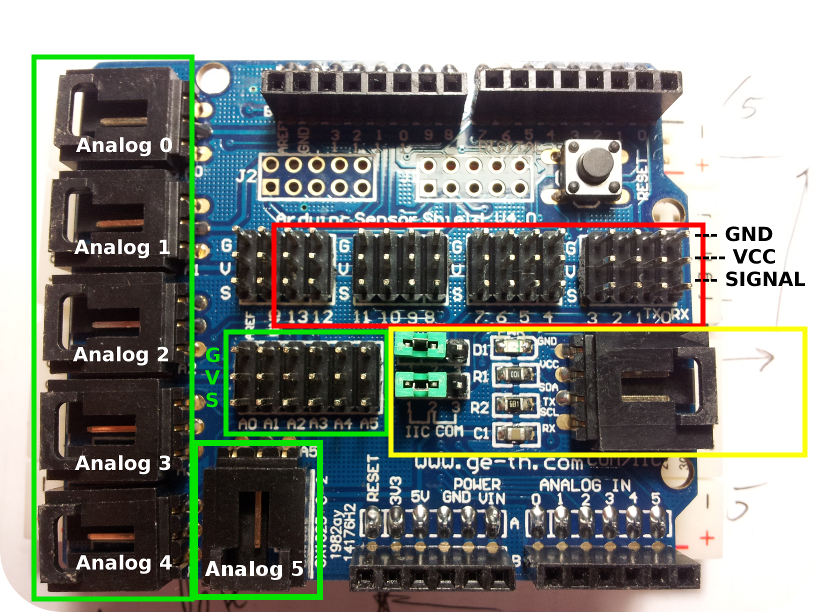
\includegraphics[width=10cm]{w_09_2016_Sklipus3.png}
  \caption {Sensor shield v4}\label{Sklipus3}
\end{figure}


Мотор подключить к Arduino напрямую не получится. Нужно использовать специальные Motor Driver. Сейчас из достаточно много в продаже, и есть инструкции по подключению. Я использовал Motor Driver, разработанный в нашей лаборатории (рис. ~\ref{Sklipus4}).

\begin{figure}[h!]
  \centering
  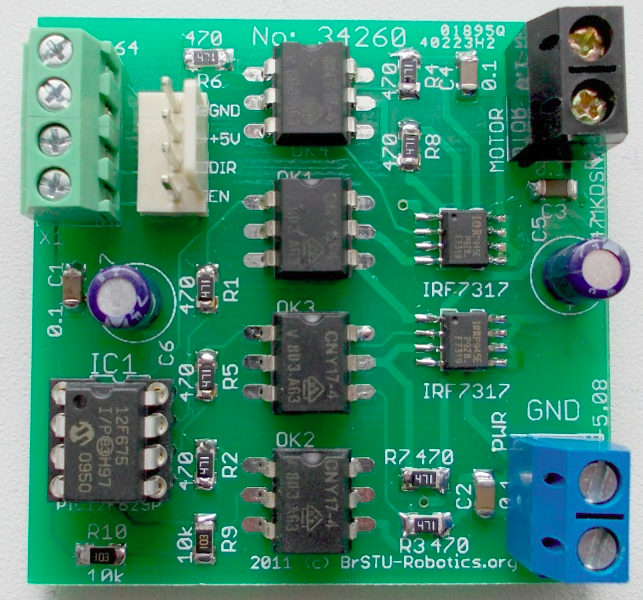
\includegraphics[width=10cm]{w_09_2016_Sklipus4.png}
  \caption {Motor driver}\label{Sklipus4}
\end{figure}


В соревнованиях роботов приходится много внимания уделять батареям. Я использую литий-полимерные аккумуляторы. Они \linebreak очень хорошо себя зарекомендовали. Один из хаков, которые я применяю в своем роботе, касается преобразователя напряжения. Штатный преобразователь в Arduino не очень хорош, поэтому для экономии энергии аккумулятора неплохо использовать Step-Down регулятор~\cite{Sklipus2}. Конечно, можно использовать и обычный линейный преобразователь.

Самая главная часть робота это датчики "--- то, что обеспечивает его информацией об окружающем мире, о препятствиях и о других роботах. В средней ценовой категории мы можем выбирать из \emph{ультразвуковых} и \emph{инфракрасных} датчиков. В своем роботе я использую инфракрасные датчики GP2Y0A02YK0F. Мне не нравятся ультразвуковые датчики из-за того, что может происходить зашумление одного датчика другим. Например, у меня возникали такие ситуации: правый датчик посылал сигнал, а левый его принимал. Я все ещё работаю над правильным размещением ультразвуковых датчиков и над управлением ими. Надежду их запустить постоянно подпитывает их цена.

На представленной здесь модели робота установлено три инфракрасных датчика. Датчики можно увидеть на рисунке ~\ref{Sklipus2}. Они установлены в глубь корпуса по двум причинам:

\begin{enumerate}
  \item для уменьшения мертвой зоны датчика, которая у данной модели составляет 20 см;
  \item корпус робота защищает датчики от механических повреждений во время столкновений с другими роботами.
\end{enumerate}

Боковые датчики установлены под углом 45 градусов. Хорошо, если в конструкции робота предусмотрена регулировка угла их установки.
Общую схему робота можно посмотреть на рисунке ~\ref{Sklipus5}.

\begin{figure}[h!]
  \centering
  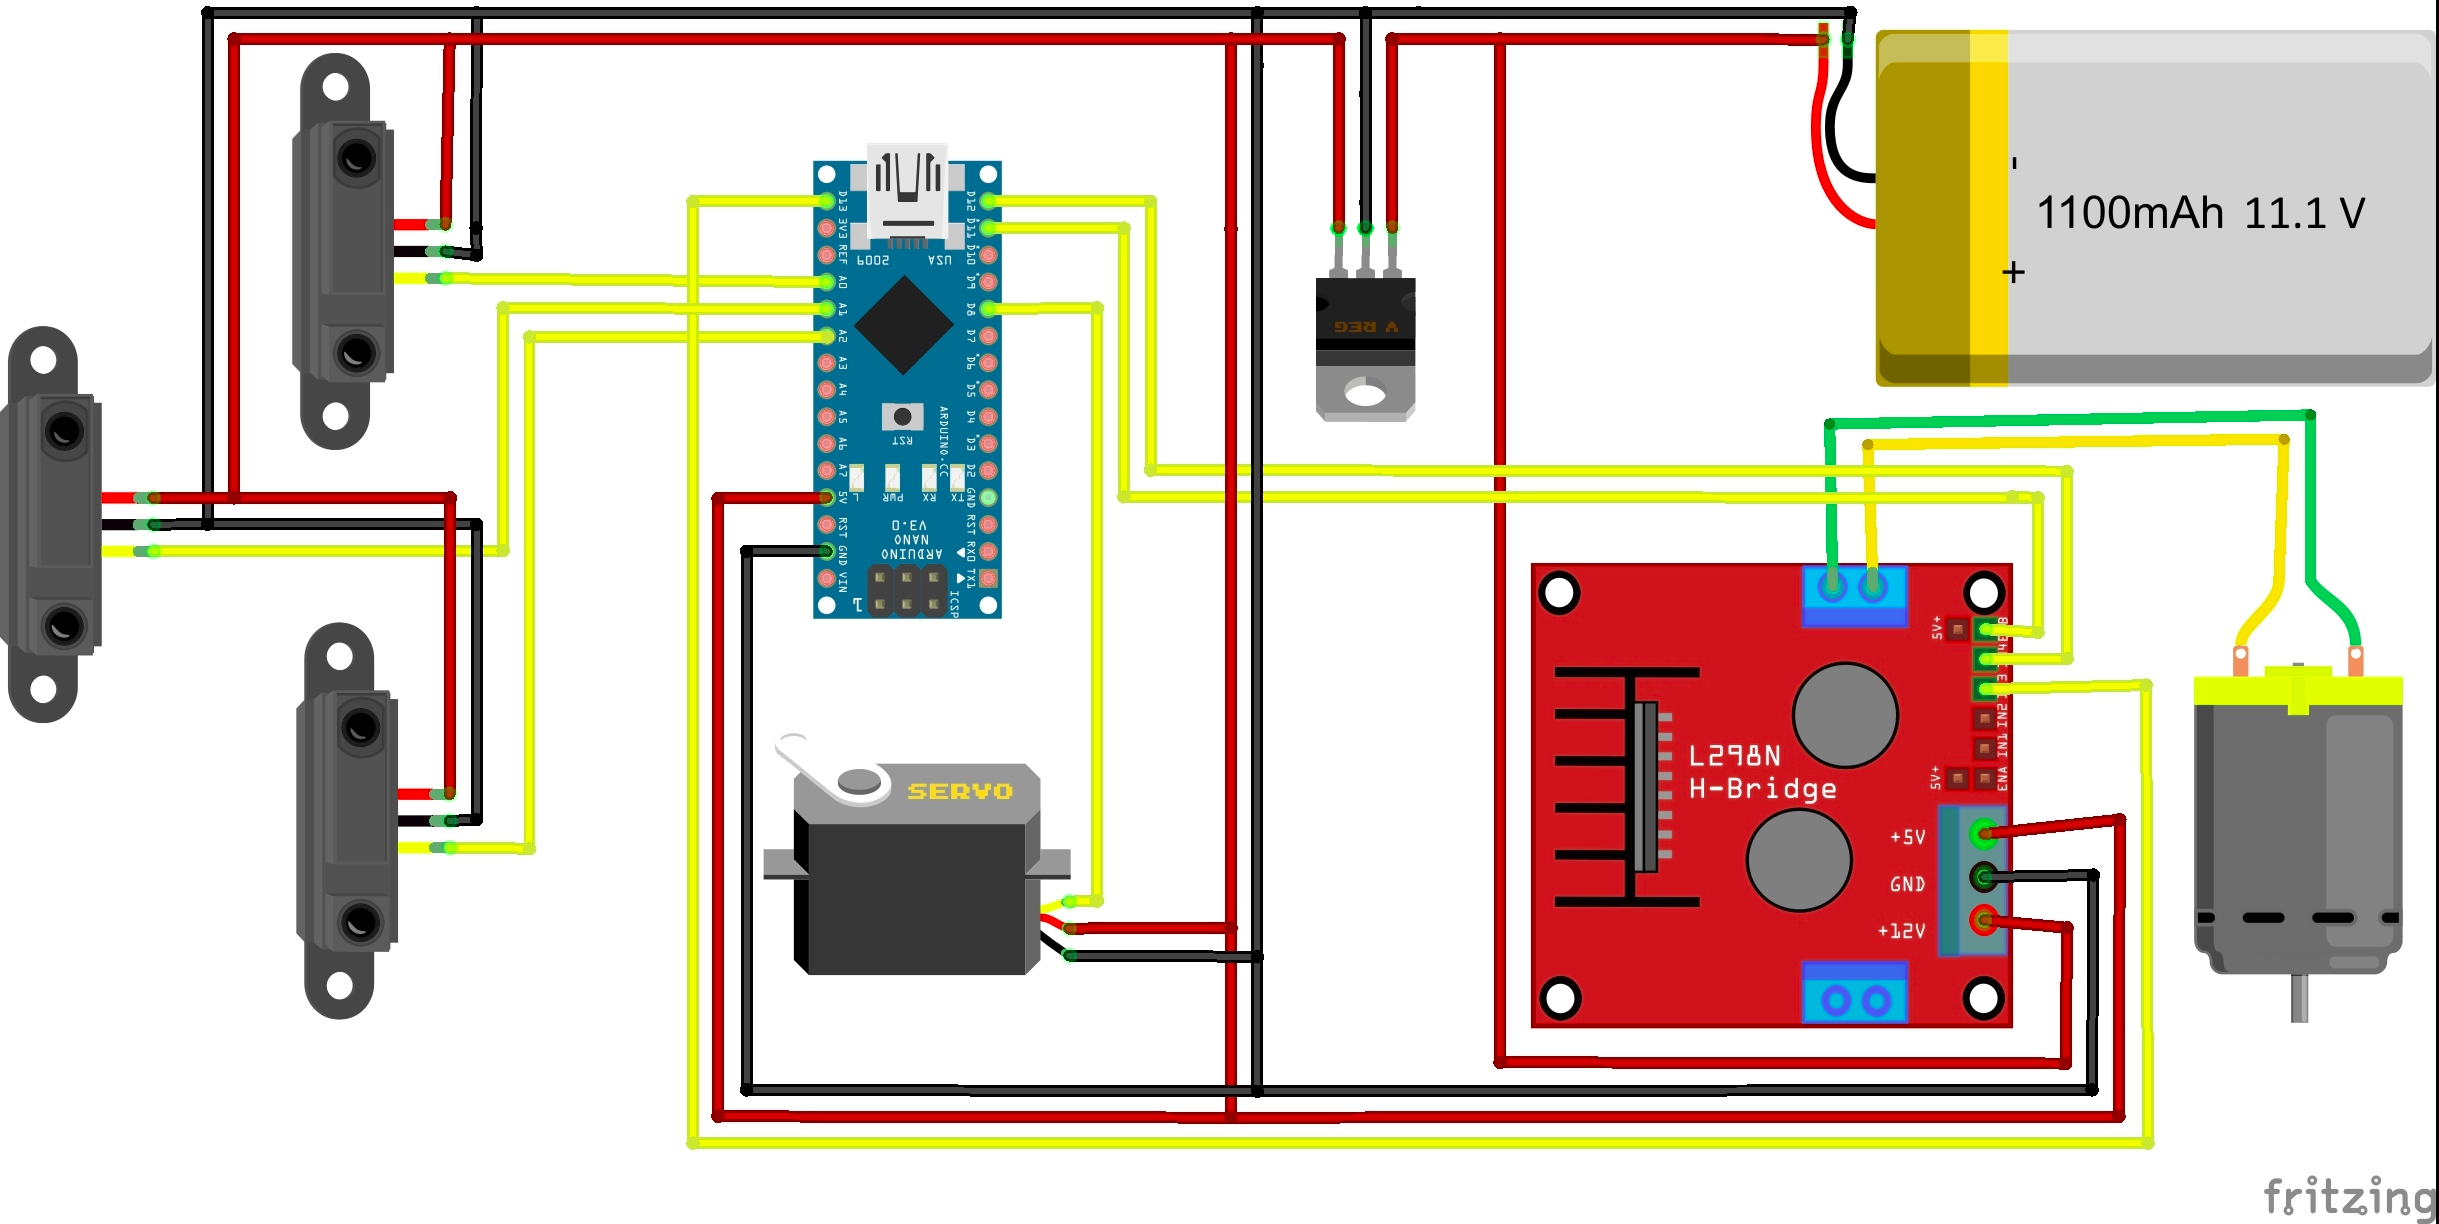
\includegraphics[width=10cm]{w_09_2016_Sklipus5.png}
  \caption {Общая схема робота}\label{Sklipus5}
\end{figure} 

\subsection*{Программирование робота}

Так как на роботе используется Arduino, то программирование выполняется с использованием Arduino IDE. Программа робота представляет собой замкнутый цикл, который состоит из следующих блоков:

\begin{enumerate}
  \item Фильтрация показаний датчиков;
  \item Вычисление угла и скорости движения робота;
  \item Передача управляющих сигналов на механизмы.
\end{enumerate}

В данной структуре отсутствует блок получения информации от датчиков. Так как датчики возвращают аналоговый сигнал, в Arduino IDE есть функция analogWrite(). Данная функция замечательно работает, если не важна скорость измерения. Но так как робот разрабатывался для соревнований, было принято решение вынести обработку датчиков в прерывание.

Все  платы Arduino, построенные на микроконтроллере ATmega, имеют возможность проводить измерения АЦП в автоматическом режиме. Нужно один раз настроить этот режим, а потом пользоваться полученными значениями. В результате контроллер постоянно проверяет датчики, не тратя на это процессорное время. Фильтрация показаний датчиков осуществляется медианным фильтром с окном в три элемента.

Для движения по трассе был выработан следующий алгоритм. Робот сравнивает расстояния до правой и левой стенки, и в соответствии с этим поворачивает колеса в нужное направление. Если впереди робота нет препятствий, скорость  увеличивается, но также уменьшается максимально возможный угол поворота колес. Это нужно для того, чтобы на прямых участках робот ехал более прямо. При обнаружении препятствия угол поворота колес увеличивается, и робот притормаживает.

Есть конечно и нерешенные проблемы. Например, робот не знает кривизну поворота, поэтому тормозит перед каждым поворотом.

Посмотреть код проекта можно на GitHub~\cite{Sklipus}.

\begin{thebibliography}{99}

\bibitem{Sklipus1} \url{https://en.wikipedia.org/wiki/Servo\_\%28radio\_control\%29}
\bibitem{Sklipus2} \url{https://www.google.com/url?q=https\%3A\%2F\%2Fsites.google.com\%2Fsite\%2Fsklipusrobotsystems\%2Fhardware\%2Fpower-of-robot\&sa=D\&sntz=1\&usg=AFQjCNHdVp\_jzQoLmZ8pIL3PrrfXRarkuA}
\bibitem{Sklipus3} \url{https://github.com/sklipus/roborace/tree/master/robots/FreshSRDEDITION}
\end{thebibliography}

\end{document}

\documentclass[10pt, a5paper]{article}
\usepackage{pdfpages}
\usepackage{parallel}
\usepackage[T2A]{fontenc}
\usepackage{ucs}
\usepackage[utf8x]{inputenc}
\usepackage[polish,english,russian]{babel}
\usepackage{hyperref}
\usepackage{rotating}
\usepackage[inner=2cm,top=1.8cm,outer=2cm,bottom=2.3cm,nohead]{geometry}
\usepackage{listings}
\usepackage{graphicx}
\usepackage{wrapfig}
\usepackage{longtable}
\usepackage{indentfirst}
\usepackage{array}
\newcolumntype{P}[1]{>{\raggedright\arraybackslash}p{#1}}
\frenchspacing
\usepackage{fixltx2e} %text sub- and superscripts
\usepackage{icomma} % коскі ў матэматычным рэжыме
\PreloadUnicodePage{4}

\newcommand{\longpage}{\enlargethispage{\baselineskip}}
\newcommand{\shortpage}{\enlargethispage{-\baselineskip}}

\def\switchlang#1{\expandafter\csname switchlang#1\endcsname}
\def\switchlangbe{
\let\saverefname=\refname%
\def\refname{Літаратура}%
\def\figurename{Іл.}%
}
\def\switchlangen{
\let\saverefname=\refname%
\def\refname{References}%
\def\figurename{Fig.}%
}
\def\switchlangru{
\let\saverefname=\refname%
\let\savefigurename=\figurename%
\def\refname{Литература}%
\def\figurename{Рис.}%
}

\hyphenation{admi-ni-stra-tive}
\hyphenation{ex-pe-ri-ence}
\hyphenation{fle-xi-bi-li-ty}
\hyphenation{Py-thon}
\hyphenation{ma-the-ma-ti-cal}
\hyphenation{re-ported}
\hyphenation{imp-le-menta-tions}
\hyphenation{pro-vides}
\hyphenation{en-gi-neering}
\hyphenation{com-pa-ti-bi-li-ty}
\hyphenation{im-pos-sible}
\hyphenation{desk-top}
\hyphenation{elec-tro-nic}
\hyphenation{com-pa-ny}
\hyphenation{de-ve-lop-ment}
\hyphenation{de-ve-loping}
\hyphenation{de-ve-lop}
\hyphenation{da-ta-ba-se}
\hyphenation{plat-forms}
\hyphenation{or-ga-ni-za-tion}
\hyphenation{pro-gramming}
\hyphenation{in-stru-ments}
\hyphenation{Li-nux}
\hyphenation{sour-ce}
\hyphenation{en-vi-ron-ment}
\hyphenation{Te-le-pathy}
\hyphenation{Li-nux-ov-ka}
\hyphenation{Open-BSD}
\hyphenation{Free-BSD}
\hyphenation{men-ti-on-ed}
\hyphenation{app-li-ca-tion}

\def\progref!#1!{\texttt{#1}}
\renewcommand{\arraystretch}{2} %Іначай формулы ў матрыцы зліпаюцца з лініямі
\usepackage{array}

\def\interview #1 (#2), #3, #4, #5\par{

\section[#1, #3, #4]{#1 -- #3, #4}
\def\qname{LVEE}
\def\aname{#1}
\def\q ##1\par{{\noindent \bf \qname: ##1 }\par}
\def\a{{\noindent \bf \aname: } \def\qname{L}\def\aname{#2}}
}

\def\interview* #1 (#2), #3, #4, #5\par{

\section*{#1\\{\small\rm #3, #4. #5}}

\def\qname{LVEE}
\def\aname{#1}
\def\q ##1\par{{\noindent \bf \qname: ##1 }\par}
\def\a{{\noindent \bf \aname: } \def\qname{L}\def\aname{#2}}
}

\begin{document}
\title{Использование архитектуры  EAV в Opensource-проектах\footnote{\url{vitalyok@tut.by}, \url{http://lvee.org/ru/abstracts/172}}}
\author{Виталий Сороко, Гродно, Беларусь}
\maketitle
\begin{abstract}
Entity–attribute–value model (EAV) is a very flexible data model used in various open source projects. This data model has many advantages and disadvantages so it is not suitable for wide application. But sometimes it is highly recommended to use EAV in design and development process.

Cases are decribed, in which it is preferable to use EAV data model. EAV is completely compared with the standard relational data model and  some examples of  successfully integration EAV in ready-to-use open source solutions are given.
\end{abstract}

Entity–attribute–value model (EAV) – это модель данных, которая благодаря использованию сущностей, атрибутов и их значений обеспечивает большую гибкость при создании новых данных. Это означает, что при создании нового типа товара в интернет магазине нет никакой необходимости создавать новые таблицы и поля в базе данных. Более того благодаря использованию этой модели данных можно с лёгкостью создать один товар из нескольких уже существующих (например «подарочный набор»). Тем не менее использование модели  EAV не ограничивается только интернет магазинами: некоммерческая организация Apache Software Foundation использует её в проекте Apache UIMA, а некоторые системы баз данных, такие как InfinityDB, изначально имеют поддержку модели данных EAV.

\begin{figure}[h!]
  \centering
  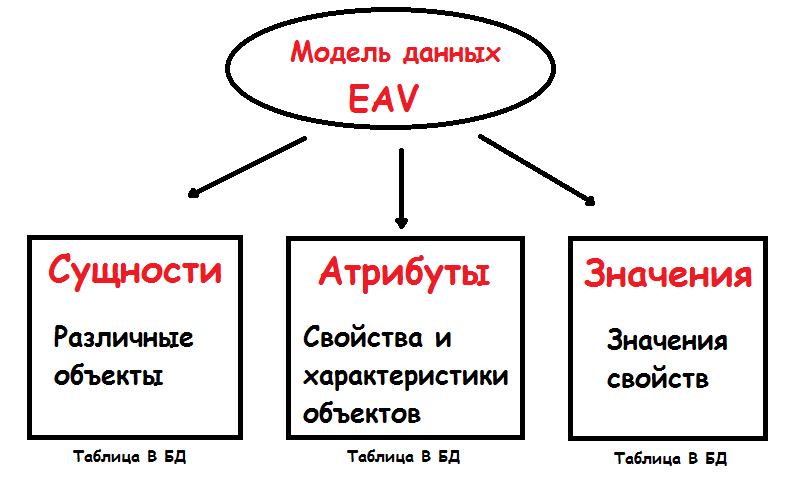
\includegraphics[width=10cm]{w_10_2016_Soroko1.png}
  \caption {Общая схема EAV в виде трёх таблиц}\label{Soroko1}
\end{figure} 

Тем не менее у модели данных EAV, как и у всех других моделей данных, есть свои преимущества и недостатки и это в некоторых случаях ограничивает возможность использования данной модели.

Главными плюсами модели данных EAV являются:

\begin{enumerate}
\item Гибкая и универсальная структура данных (можно менять количество свойств без изменения полей в таблицах);
\item Относительная простота при добавлении или изменении характеристики товара;
\item При правильной реализации избыточность данных почти отсутствует.
\end{enumerate}

Основные минусы EAV:
\begin{enumerate}
\item Для вставки данных обычно используется несколько запросов;
\item Не очень быстрая выборка данных в случае реализации с большим количеством таблиц и высокая нагрузка на сервер при больших объемах данных в связи с невозможностью применения стандартных способов индексации;
\item Иногда возникают трудности в обеспечении целостности данных.
\end{enumerate}

\begin{figure}[h!]
  \centering
  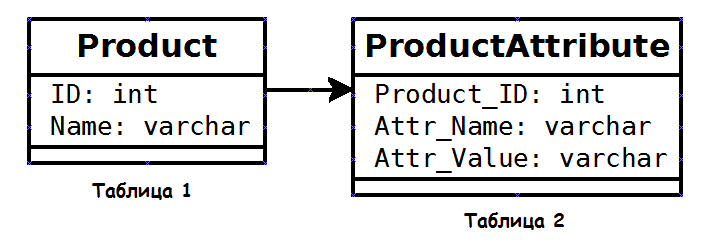
\includegraphics[width=10cm]{w_10_2016_Soroko2.png}
  \caption {Простейшая реализация EAV в виде двух таблиц}\label{Soroko2}
\end{figure} 

В настоящее время модель данных EAV используется в таких Opensource проектах как  Magento Community Edition, EAV-Django и др.  Необходимо отметить, что модель данных EAV не получила очень широкого распространения не только из-за своих технических минусов, но также в результате её неполного понимания со стороны разработчиков. Как правило только те, кто разобрался с принципом работы этой модели и попробовал её в реальной среде, могут объективно судить о её преимуществах и недостатках,  а также рекомендовать её к использованию в той или иной ситуации и именно поэтому, очень важно полностью понять основные принципы  организации её работы. В упрощённом виде реализация модели EAV может быть в виде двух или трех таблиц (см. рис.~\ref{Soroko1} и рис.~\ref{Soroko2}).

Однако в реальных проектах реализация обычно сложнее, и на то есть определенные причины, такие как оптимизация скорости обработки запросов и уменьшение общего количества записей в таблицах.Так, например, в Magento CMS CE для реализации данной модели используется больше десятка таблиц. Как вы могли узнать из описание недостатков выше, иногда гибкость может трансформироваться в падение производительности всей системы. Тем не менее, в настоящее время уже разработаны различные способы решения этой проблемы. Итого, главная рекомендация по применению следующая: EAV рекомендуется использовать только исходя из плюсов, а именно в случаях если характеристики для товаров очень динамичны и часто изменяются и вы не ограничены в серверных ресурсах.

\end{document}

\documentclass[10pt, a5paper]{article}
\usepackage{pdfpages}
\usepackage{parallel}
\usepackage[T2A]{fontenc}
\usepackage{ucs}
\usepackage[utf8x]{inputenc}
\usepackage[polish,english,russian]{babel}
\usepackage{hyperref}
\usepackage{rotating}
\usepackage[inner=2cm,top=1.8cm,outer=2cm,bottom=2.3cm,nohead]{geometry}
\usepackage{listings}
\usepackage{graphicx}
\usepackage{wrapfig}
\usepackage{longtable}
\usepackage{indentfirst}
\usepackage{array}
\newcolumntype{P}[1]{>{\raggedright\arraybackslash}p{#1}}
\frenchspacing
\usepackage{fixltx2e} %text sub- and superscripts
\usepackage{icomma} % коскі ў матэматычным рэжыме
\PreloadUnicodePage{4}

\newcommand{\longpage}{\enlargethispage{\baselineskip}}
\newcommand{\shortpage}{\enlargethispage{-\baselineskip}}

\def\switchlang#1{\expandafter\csname switchlang#1\endcsname}
\def\switchlangbe{
\let\saverefname=\refname%
\def\refname{Літаратура}%
\def\figurename{Іл.}%
}
\def\switchlangen{
\let\saverefname=\refname%
\def\refname{References}%
\def\figurename{Fig.}%
}
\def\switchlangru{
\let\saverefname=\refname%
\let\savefigurename=\figurename%
\def\refname{Литература}%
\def\figurename{Рис.}%
}

\hyphenation{admi-ni-stra-tive}
\hyphenation{ex-pe-ri-ence}
\hyphenation{fle-xi-bi-li-ty}
\hyphenation{Py-thon}
\hyphenation{ma-the-ma-ti-cal}
\hyphenation{re-ported}
\hyphenation{imp-le-menta-tions}
\hyphenation{pro-vides}
\hyphenation{en-gi-neering}
\hyphenation{com-pa-ti-bi-li-ty}
\hyphenation{im-pos-sible}
\hyphenation{desk-top}
\hyphenation{elec-tro-nic}
\hyphenation{com-pa-ny}
\hyphenation{de-ve-lop-ment}
\hyphenation{de-ve-loping}
\hyphenation{de-ve-lop}
\hyphenation{da-ta-ba-se}
\hyphenation{plat-forms}
\hyphenation{or-ga-ni-za-tion}
\hyphenation{pro-gramming}
\hyphenation{in-stru-ments}
\hyphenation{Li-nux}
\hyphenation{sour-ce}
\hyphenation{en-vi-ron-ment}
\hyphenation{Te-le-pathy}
\hyphenation{Li-nux-ov-ka}
\hyphenation{Open-BSD}
\hyphenation{Free-BSD}
\hyphenation{men-ti-on-ed}
\hyphenation{app-li-ca-tion}

\def\progref!#1!{\texttt{#1}}
\renewcommand{\arraystretch}{2} %Іначай формулы ў матрыцы зліпаюцца з лініямі
\usepackage{array}

\def\interview #1 (#2), #3, #4, #5\par{

\section[#1, #3, #4]{#1 -- #3, #4}
\def\qname{LVEE}
\def\aname{#1}
\def\q ##1\par{{\noindent \bf \qname: ##1 }\par}
\def\a{{\noindent \bf \aname: } \def\qname{L}\def\aname{#2}}
}

\def\interview* #1 (#2), #3, #4, #5\par{

\section*{#1\\{\small\rm #3, #4. #5}}

\def\qname{LVEE}
\def\aname{#1}
\def\q ##1\par{{\noindent \bf \qname: ##1 }\par}
\def\a{{\noindent \bf \aname: } \def\qname{L}\def\aname{#2}}
}

\begin{document}
\title{Опыт использования СПО в учебном процессе УРТК им. А.С. Попова}
\author{Anton Uymin, Arseny Meshkov, Yekaterinburg, Russia}
\maketitle
\begin{abstract}
The article describes experience of adopting free software in a secondary vocational educational institution - a college. List of profession specialties and specialized classrooms that use free software is presented. Advantages and disadvantages of using free software in the educational process are discussed.
\end{abstract}
В настоящее время в Российском образовании складывается сложная ситуация. С одной стороны, идет активная реформа по преобразованию учебных заведений, их укрупнению и консолидации ресурсов, с другой стороны среднее профессиональное образование и высшее образование уже не дополняют друг друга, как это было ранее, а являются прямыми конкурентами на рынке образовательных услуг. При этом уровень финансирования СПО и ВПО отличается на порядки. Сегодня образовательное учреждение не может выжить, если будет предоставлять парты и доски, необходим качественно новый уровень технического и методического обеспечения. Каждый студент может получить полный объём информации в интернете, но он не может её качественно классифицировать и, зачастую, у него нет хорошей базы оборудования для изучения современных технологий. Поэтому ОУ сейчас не столько должны нести новые знания, сколько предоставлять платформу для образовательной деятельности.

<<СПО для нищебродов!>> "--- с этой фразы одного из представителей сообщества СПО в Екатеринбурге хотелось бы начать данную статью. Уральский радиотехнический колледж им. А.С. Попова находится в Екатеринбурге. У нас реализуется всего 12 специальностей. Из них 6 "--- по IT-направлению. До 2008 года в нашем учебном заведении из СПО были шлюз и сайт на FreeBSD. В учебном процессе СПО не использовалось никак. В 2008 году мы начали сотрудничать с отделом <<К>>, консультировались у них, отправляли к ним на практику студентов. В этом же году начался перевод учебных материалов на Linux.

В колледже 19 компьютерных лабораторий. Парк ПК насчитывает около 500 шт. Парк серверов 20 шт. Обслуживанием лабораторий занимаются заведующие лабораториями, которые являются и преподавателями спец. дисциплин.

Первой лабораторией, переведенной на Linux, стала лаборатория 104 <<Программно-аппаратной защиты объектов сетевой инфраструктуры>>. Выбор дистрибутива, который окажется штатным в лаборатории был долгим и сложным. Мы прошли путь от FreeBSD \textgreater{} PC-BSD \textgreater{} Debian \textgreater{} Fedora \textgreater{} Alt Linux. У Alt Linux подкупила простота начального вхождения, качество документирования и форум, на котором действительно помогают. Мы начали с Alt Linux Школьный Новый Легкий, сейчас работаем на Alt Linux Centaurus P7 и с нетерпением ждем выхода 8 платформы.

В таблице \ref{Uymin1} приведён перечень лабораторий и указан год перехода на СПО. Во всех лабораториях расположено по 12 рабочих мест студентов, кроме 304, где 27 раб. мест.


\begin{longtable}[h!]{|p{0.7cm}|p{2cm}|p{1cm}|p{2.5cm}|p{2.5cm}|}
\caption{Перечень лабораторий} \label{Uymin1} \\
\hline

\textbf{№} & \textbf{Название лаборатории} & \textbf{Год перехода} & \textbf{Преподаются дисциплины связанные с} & \textbf{На рабочем месте студента} \\
\hline
\endfirsthead % конец заголовка на первой странице

\hline
\textbf{№} (продолжение) & \textbf{Название лаборатории} (продолжение) & \textbf{Год перехода} (продолжение) & \textbf{Преподаются дисциплины связанные с} (продолжение) & \textbf{На рабочем месте студента} (продолжение) \\
\hline
\endhead % заголовок для других страниц 

 101 & Сборки, монтажа и эксплуатации средств вычислительной техники &  2012 & аппаратным обеспечением ПЭВМ. Установка, настройка системного ПО, развертывание служб и сервисов. Техническое обслуживание и ремонт СВТ. & ПЭВМ, принтер, сканер \\ 
\hline 
 104 & Программно-аппаратной защиты объектов сетевой инфраструктуры & 2009 & сетевыми операционными системами, информационной безопасностью. &  2 ПЭВМ, на которых студенты развертывают несколько сетей в системах виртуализации. \\ 
\hline 
 114 & Сетевая академия Cisco. & 2013 & сетевыми технологиями в рамках Cisco CCNA. &  ПЭВМ \\ 
\hline 
 117 & Лаборатория беспроводных технологий & 2014 & сетевыми технологиями: беспроводные сети. & ПЭВМ, с дискретными беспроводными и проводными адаптерами и видеокартой Radeon для анализа защищенности беспроводных соединений. В стенд входят два беспроводных маршрутизатора и ip-камера. \\
\hline 
 304 & Информати~\-ки. Программирования и баз данных &  2015 & информатикой и программированием. & ПЭВМ \\ 
\hline 
 305 & Программно~\-го обеспечения компьютерных сетей. Авторизованный центр Cisco Academy & 2015 & основами компьютерной грамотности. & ПЭВМ \\
\hline 

\end{longtable}

Есть участки, на которых нет возможности перейти на СПО и приходится использовать Windows. В связи с тем, что мы обучаем для конкретных предприятий и организаций, то прикладное ПО диктуют они. Используются такие программные пакеты как Altium Designer, Autodesk Autocad, MS Office, 1С и т.д.

Стандартным пакетом дополнительного ПО в лабораториях является: Remmina, Firefox, Geany, iTALC, OpenSSH, PuTTY, \linebreak VirtualBox.

К нестандартному относятся такие пакеты как Cisco Packet Tracer, LinSSID, Aircrack-ng, Wireshark, Metasploit Framework.

Сервисы на базе СПО, используемые для обслуживания образовательного процесса, приведены в таблице \ref{Uymin2}.

\begin{longtable}[h!]{|p{3cm}|p{3cm}|p{3cm}|}
\caption{Используемые сервисы} \label{Uymin2} \\
\hline

\textbf{Сервис} & \textbf{На чем настроен} & \textbf{Назначение} \\
\hline
\endfirsthead % конец заголовка на первой странице

\hline
\textbf{Сервис} (продолжение) & \textbf{На чем настроен} (продолжение) & \textbf{Назначение} (продолжение) \\
\hline
\endhead % заголовок для других страниц 

    Система видеонаблюдения &  Debian 7 + MotionEye & Обеспечение безопасности функционирования лабораторий, отслеживание инцидентов \\
\hline
    Локальное зеркало репозиториев Debian & Debian 7 + apt-mirror & Проведение лабораторных работ \\
\hline
    Локальное зеркало репозиториев Alt Linux & Alt Linux P7 + sisyphus-mirror & Обслуживание ПЭВМ \\
\hline
    Сервер сетевой загрузки & Debian 7 + tftpd-hpa + isc-dhcp-server + syslinux + nfs-kernel-server + smb + apache2 & Обслуживание ПЭВМ \\
\hline
    Вики-энциклопедия & Alt Linux P7 + Mediawiki & Создание и хранение документации \\
\hline
    Сервер SNMP-мониторинга & Debian 8 + Zabbix & Мониторинг сетевого оборудования \\
\hline
    Система дистанционного обучения & FreeBSD 7 + Moodle & СДО \\
\hline

\end{longtable}

Сервер сетевой загрузки позволяет производить загрузку следующих образов ОС – Debian 8, Alt Linux P7, Windows 7/8.1/2012R2, а так же системных и служебных утилит HDT, memtest86+, MS DaRT, MHDD. 
В 2016 году планируется развёртывание \linebreak LDAP-домена на базе Alt Linux с целью централизованного управления правами студентов в лабораториях и обеспечения непрерывной рабочей среды, так же мы начали сотрудничество с компанией РусБИТех, запланирована организация учебных мест на базе Astra Linux SE.

УРТК им. А.С. Попова пытается стать образовательной площадкой, на базе которой  студенты имеют возможность поработать на современном сетевом оборудовании "--- (учебные классы таких вендоров как Cisco, D-Link, TP-Link) с современным программным и аппаратным обеспечением "--- (ПЭВМ i7/16Gb/1Tb для развертывания виртуальных машин – в зависимости от лабораторной работы от 1 до 8 шт. для каждого студента). Кроме этого, мы стараемся держать инфраструктуру колледжа в актуальном состоянии, т.е. систематически добавлять новые интересные сервисы в процесс технического обслуживания образовательного процесса. СПО нам в этом неоценимо помогает, т.к. позволяет активно изучать интересные пакеты и сервисы, оптимально по денежным вложениям и нетребовательно по аппаратным ресурсам, а самое главное, доступно для различных дополнений и модификаций  под конкретные задачи.

\textbf{Вместо вывода:}

\begin{enumerate}
  \item Свободное программное обеспечение позволяет будущим специалистам более глубоко изучать технологии: если студент смог настроить DNS на Linux, то у него не возникнет проблем при аналогичных настройках на Windows или сетевом оборудовании.
  \item Кризис и санкции стимулировали внедрение СПО в СПО. Например, до 2015 года руководство особого интереса не проявляло, а в 2015 году мы выступали перед советом директоров ССУЗов Свердловской области с докладом о практике внедрения свободного программного обеспечения в нашем колледже.
  \item Свободное программное обеспечение сложнее в развёртывании, настройке и обслуживании. Руководство не готово оплачивать ни полноценную техническую поддержку ни доплачивать за обслуживание СПО, что влияет на мотивацию технического персонала.
  \item Так как у Linux отсутствует маркетинговая поддержка, то затруднительно агитировать и продвигать свободные технологии в массы. Например, колледж проводит много различных мероприятий: областные и международные олимпиады. С одной стороны, поддержку данным мероприятиям готовы оказать только люди, интересующиеся СПО в частном порядке. Компании и вендоры не готовы оказывать поддержку. С другой стороны, большое количество учебных заведений испытывают трудности при подготовке студентов к заданиям с использованием CПО.
  \item К сожалению, мы <<нищеброды>>, которые пытаются готовить профессионалов, в чём СПО нам активно помогает.
\end{enumerate}

\end{document}

\documentclass[10pt, a5paper]{article}
\usepackage{pdfpages}
\usepackage{parallel}
\usepackage[T2A]{fontenc}
\usepackage{ucs}
\usepackage[utf8x]{inputenc}
\usepackage[polish,english,russian]{babel}
\usepackage{hyperref}
\usepackage{rotating}
\usepackage[inner=2cm,top=1.8cm,outer=2cm,bottom=2.3cm,nohead]{geometry}
\usepackage{listings}
\usepackage{graphicx}
\usepackage{wrapfig}
\usepackage{longtable}
\usepackage{indentfirst}
\usepackage{array}
\newcolumntype{P}[1]{>{\raggedright\arraybackslash}p{#1}}
\frenchspacing
\usepackage{fixltx2e} %text sub- and superscripts
\usepackage{icomma} % коскі ў матэматычным рэжыме
\PreloadUnicodePage{4}

\newcommand{\longpage}{\enlargethispage{\baselineskip}}
\newcommand{\shortpage}{\enlargethispage{-\baselineskip}}

\def\switchlang#1{\expandafter\csname switchlang#1\endcsname}
\def\switchlangbe{
\let\saverefname=\refname%
\def\refname{Літаратура}%
\def\figurename{Іл.}%
}
\def\switchlangen{
\let\saverefname=\refname%
\def\refname{References}%
\def\figurename{Fig.}%
}
\def\switchlangru{
\let\saverefname=\refname%
\let\savefigurename=\figurename%
\def\refname{Литература}%
\def\figurename{Рис.}%
}

\hyphenation{admi-ni-stra-tive}
\hyphenation{ex-pe-ri-ence}
\hyphenation{fle-xi-bi-li-ty}
\hyphenation{Py-thon}
\hyphenation{ma-the-ma-ti-cal}
\hyphenation{re-ported}
\hyphenation{imp-le-menta-tions}
\hyphenation{pro-vides}
\hyphenation{en-gi-neering}
\hyphenation{com-pa-ti-bi-li-ty}
\hyphenation{im-pos-sible}
\hyphenation{desk-top}
\hyphenation{elec-tro-nic}
\hyphenation{com-pa-ny}
\hyphenation{de-ve-lop-ment}
\hyphenation{de-ve-loping}
\hyphenation{de-ve-lop}
\hyphenation{da-ta-ba-se}
\hyphenation{plat-forms}
\hyphenation{or-ga-ni-za-tion}
\hyphenation{pro-gramming}
\hyphenation{in-stru-ments}
\hyphenation{Li-nux}
\hyphenation{sour-ce}
\hyphenation{en-vi-ron-ment}
\hyphenation{Te-le-pathy}
\hyphenation{Li-nux-ov-ka}
\hyphenation{Open-BSD}
\hyphenation{Free-BSD}
\hyphenation{men-ti-on-ed}
\hyphenation{app-li-ca-tion}

\def\progref!#1!{\texttt{#1}}
\renewcommand{\arraystretch}{2} %Іначай формулы ў матрыцы зліпаюцца з лініямі
\usepackage{array}

\def\interview #1 (#2), #3, #4, #5\par{

\section[#1, #3, #4]{#1 -- #3, #4}
\def\qname{LVEE}
\def\aname{#1}
\def\q ##1\par{{\noindent \bf \qname: ##1 }\par}
\def\a{{\noindent \bf \aname: } \def\qname{L}\def\aname{#2}}
}

\def\interview* #1 (#2), #3, #4, #5\par{

\section*{#1\\{\small\rm #3, #4. #5}}

\def\qname{LVEE}
\def\aname{#1}
\def\q ##1\par{{\noindent \bf \qname: ##1 }\par}
\def\a{{\noindent \bf \aname: } \def\qname{L}\def\aname{#2}}
}

\begin{document}
\title{Практическая индивидуальная настройка клавиатуры в GNU/Linux}
\author{Александра Игоревна Кононова, Алексей Владиславович Городилов, Олег Олегович Кондрашов Москва, г. Зеленоград, РФ}
\maketitle
\begin{abstract}
xkb (X Keyboard Extension) possibilities are not limited to keyboard layout selection and switching from predefined list.
With xkb it is possible to create custom layouts with necessary symbols and modifiers, assign up to 8 symbols to a single key. It is also possible to set up non-cyclic layouts switching, re-assign keys of auxiliary keyboards (e. g. gaming mouse keyboard), change layouts on-the-fly, combine symbol entry and layout switch in one key, etc.
\end{abstract}

В настоящее время наиболее распространённой оконной системой для построения графического интерфейса пользователя в UNIX-подобных ОС является X Window System. Для работы с клавиатурой предназначена одна из подсистем X Window System "--- xkb. 
Чаще всего пользователь X Window System встречается с xkb при настройке поддержки русского ввода. Но её возможности не ограничиваются выбором раскладки и переключателя раскладки из предопределённого разработчиком дистрибутива списка вариантов. Подробное описание настройки xkb доступно на сайте Ивана Паскаля ~\cite{Kononova1}. Рассмотрим практическое применение некоторых возможностей этой подсистемы.

\subsection*{Ввод символов}

Часто возникает необходимость вставить в текст символ, отсутствующий в используемых раскладках, в частности, тире и кавычки, соответствующие правилам русской типографики. Подсистема xkb предлагает четыре основных способа набора таких символов.

\begin{enumerate}
  \item Указание кода символа в Unicode (в частности, в соответствии с ISO 14755).
Позволяет ввести любой существующий символ, но для этого требуется помнить этот код, что не очень удобно. Кроме того, способ задания кода может различаться для разных приложений.
  \item Compose-последовательности.
Чтобы ввести символ, нажимается специальная клавиша Compose и вводится цепочка символов.
  \item Использование существующей раскладки с типографскими \linebreak символами.
Типографское расширение раскладки в xkb включает так называемый третий уровень, что позволяет набрать дополнительные символы, нажав одновременно с клавишей модификатор третьего уровня.
  \item Модификация используемой раскладки.
Можно изменить существующую раскладку или создать новую, содержащую необходимые для пользователя символы.
\end{enumerate}

\subsection*{Раскладки и настройки}

Раскладки в xkb "--- файлы настроек специального вида, которые описывают символы, генерируемые клавишами. Каждый вариант раскладки "--- отдельный блок. Внутри блока описаны связанные с клавишей данные ~\cite{Kononova1}. Для большинства клавиш это символы, которые выдаются по нажатию клавиши на различных уровнях (shift levels). 
Каждому уровню может соответствовать символ, задаваемый кодом Unicode (например, U2190) или специальной константой (например, leftarrow). Файлы раскладки поддерживают комментарии в стиле C++.

Кроме печатаемых символов (цифр, букв, иных символов \linebreak Unicode), специальных констант VoidSymbol и NoSymbol, а также невизуальных символов, таких как F1-F10, Multi\_key \linebreak (Compose), XF86Back, XF86Forward, SunFront, SunProps и т. д., клавишам могут соответствовать символы и модификаторы, влияющие на состояние клавиатуры. В частности, это символы, изменяющие текущую раскладку (группу символов). 
Чтобы набрать символ второго или более высокого уровня, при нажатии на клавишу, соответствующую этому символу, зажать ещё одну или несколько клавиш "--- модификаторов  соответствующего уровня. Модификатором второго уровня является Shift. Различные модификаторы третьего уровня (а также, в блоке modifier\_mapping, добавление виртуального модификатора <<LVL3>> в группу Mod5) описаны в /usr/share/X11/xkb/symbols/level3. Аналогичным образом можно назначить модификатором третьего уровня любую другую клавишу. Символ четвёртого уровня можно получить, зажав модификатор третьего уровня и Shift вместе.

Различные модификаторы пятого уровня (и добавление модификатора <<MDSW>> в группу Mod3, что необходимо для правильной работы) описаны в файле /usr/share/X11/xkb/symbols/level5. Cпособом, аналогичным описанному в этом файле, можно назначить и любую другую клавишу.
Иногда требуется набрать на некоторой раскладке только один символ (чаще всего это символ латиницы в кириллическом тексте). Готового символа для временного включения конкретной раскладки найти пока не удалось, но эту проблему можно решить с помощью действий (actions). Номер текущей раскладки (группы) определяется суммой трёх переменных "--- base group, latched group и locked group. Их можно изменить соответствующими действиями ~\cite{Kononova1}:

\begin{verbatim}
    replace key <RALT> \{
        actions[Group1]=[ ],
        actions[Group2]=[ SetGroup(group=-1) ],
        actions[Group3]=[ SetGroup(group=-2) ],
        actions[Group4]=[ SetGroup(group=-3) ]
    \};
\end{verbatim}

Если включена первая раскладка, при нажатии правого Alt не делается ничего, если вторая "--- переменная base group уменьшается на единицу на время нажатия и т. д. Постоянное включение первой раскладки также возможно с помощью действий, для этого необходимо изменить переменную locked group. 

Некоторые из описанных дополнений к обычной раскладке работают не только в X Window System, но и в «чистой» консоли.

\subsection*{Файлы и утилиты}

Основной файл настройки клавиатуры "--- /etc/default/keyboard, задающий набор раскладок и модификаторов для всех пользователей компьютера и всех клавиатур, причём не только для xkb, но, по умолчанию, и для консоли.

Список файлов используемых раскладок (файлы должны содержаться в каталоге /usr/share/X11/xkb/symbols/) указывается в переменной \linebreak XKBLAYOUT, список блоков "--- переменной XKBVARIANT. Дополнительные модификаторы и настройки, такие, как поведение светодиодов на клавиатуре, перечисляются в переменной XKBOPTIONS.

Изменить раскладку для текущего сеанса позволяет утилита setxkbmap. Дополнительные настройки могут быть заданы через ключ -option, сам список аналогичен XKBOPTIONS.

Утилита setxkbmap позволяет задать различные раскладки для различных устройств, указав ключ -device ~\cite{Kononova2}. Это может быть полезно, в частности, при настройке игровой мыши, имеющей на боку цифровую клавиатуру. Список всех устройств ввода, в частности, клавиатур, можно получить командой  xinput с ключом list. Так как идентификаторы устройств могут меняться от сеанса к сеансу, лучше проверять этот список каждый раз при назначении раскладки.

В том случае, если желаемой конфигурации не получается добиться, комбинируя стандартные файлы, можно изменить одну из стандартных раскладок или создать в каталоге \linebreak /usr/share/X11/xkb/symbols/ новую по образцу имеющихся. Создание собственного файла раскладки обычно предпочтительнее, так как стандартные файлы могут быть перезаписаны при обновлении.

Файл раскладки должен содержать по крайней мере один блок, описывающий поведение алфавитно-цифровых клавиш. Кроме того, можно переопределить поведение таких клавиш, как пробел и «стрелки» при нажатых модификаторах третьего и пятого уровней.
Используемые модификаторы (включатели раскладки, модификаторы третьего и пятого уровня и т. д.) также могут быть описаны непосредственно в файле раскладки.

Таким образом, возможности xkb позволяют, не используя стороннее ПО, легко набирать любые необходимые символы, а также задавать индивидуальные раскладки для различных устройств.

\begin{thebibliography}{99}
\bibitem{Kononova1} Иван Паскаль. X Keyboard Extension \url{http://pascal.tsu.ru/other/xkb/}
\bibitem{Kononova2} XKB remapping \url{http://www.pixelbeat.org/docs/xkb\_remap/}
\end{thebibliography}
\end{document}

\documentclass[10pt, a5paper]{article}
\usepackage{pdfpages}
\usepackage{parallel}
\usepackage[T2A]{fontenc}
\usepackage{ucs}
\usepackage[utf8x]{inputenc}
\usepackage[polish,english,russian]{babel}
\usepackage{hyperref}
\usepackage{rotating}
\usepackage[inner=2cm,top=1.8cm,outer=2cm,bottom=2.3cm,nohead]{geometry}
\usepackage{listings}
\usepackage{graphicx}
\usepackage{wrapfig}
\usepackage{longtable}
\usepackage{indentfirst}
\usepackage{array}
\newcolumntype{P}[1]{>{\raggedright\arraybackslash}p{#1}}
\frenchspacing
\usepackage{fixltx2e} %text sub- and superscripts
\usepackage{icomma} % коскі ў матэматычным рэжыме
\PreloadUnicodePage{4}

\newcommand{\longpage}{\enlargethispage{\baselineskip}}
\newcommand{\shortpage}{\enlargethispage{-\baselineskip}}

\def\switchlang#1{\expandafter\csname switchlang#1\endcsname}
\def\switchlangbe{
\let\saverefname=\refname%
\def\refname{Літаратура}%
\def\figurename{Іл.}%
}
\def\switchlangen{
\let\saverefname=\refname%
\def\refname{References}%
\def\figurename{Fig.}%
}
\def\switchlangru{
\let\saverefname=\refname%
\let\savefigurename=\figurename%
\def\refname{Литература}%
\def\figurename{Рис.}%
}

\hyphenation{admi-ni-stra-tive}
\hyphenation{ex-pe-ri-ence}
\hyphenation{fle-xi-bi-li-ty}
\hyphenation{Py-thon}
\hyphenation{ma-the-ma-ti-cal}
\hyphenation{re-ported}
\hyphenation{imp-le-menta-tions}
\hyphenation{pro-vides}
\hyphenation{en-gi-neering}
\hyphenation{com-pa-ti-bi-li-ty}
\hyphenation{im-pos-sible}
\hyphenation{desk-top}
\hyphenation{elec-tro-nic}
\hyphenation{com-pa-ny}
\hyphenation{de-ve-lop-ment}
\hyphenation{de-ve-loping}
\hyphenation{de-ve-lop}
\hyphenation{da-ta-ba-se}
\hyphenation{plat-forms}
\hyphenation{or-ga-ni-za-tion}
\hyphenation{pro-gramming}
\hyphenation{in-stru-ments}
\hyphenation{Li-nux}
\hyphenation{sour-ce}
\hyphenation{en-vi-ron-ment}
\hyphenation{Te-le-pathy}
\hyphenation{Li-nux-ov-ka}
\hyphenation{Open-BSD}
\hyphenation{Free-BSD}
\hyphenation{men-ti-on-ed}
\hyphenation{app-li-ca-tion}

\def\progref!#1!{\texttt{#1}}
\renewcommand{\arraystretch}{2} %Іначай формулы ў матрыцы зліпаюцца з лініямі
\usepackage{array}

\def\interview #1 (#2), #3, #4, #5\par{

\section[#1, #3, #4]{#1 -- #3, #4}
\def\qname{LVEE}
\def\aname{#1}
\def\q ##1\par{{\noindent \bf \qname: ##1 }\par}
\def\a{{\noindent \bf \aname: } \def\qname{L}\def\aname{#2}}
}

\def\interview* #1 (#2), #3, #4, #5\par{

\section*{#1\\{\small\rm #3, #4. #5}}

\def\qname{LVEE}
\def\aname{#1}
\def\q ##1\par{{\noindent \bf \qname: ##1 }\par}
\def\a{{\noindent \bf \aname: } \def\qname{L}\def\aname{#2}}
}

\begin{document}
\title{Что такое SMR-диски и как их готовить}
\author{Yauhen Kharuzhy, Minsk, belarus}
\maketitle
\begin{abstract}
Brief review of Shingled Magnetic Recording (SMR) drives and status of their support in Linux is presented including projects which are currently in development supported by Seagate and HGST companies.
\end{abstract}
\subsection*{Введение}

Плотность записи на магнитные диски растёт, но расти она может не бесконечно. Текущая применяемая в накопителях технология, перпендикулярная магнитная запись, имеет теоретический предел плотности 1 Тбит/кв.дюйм.

Один из вариантов преодоления этого предела "--- так называемая черепичная магнитная запись, SMR (Shingled Magnetic \linebreak Recording). В этой технологии используется тот факт, что ширина читающей головки заметно меньше, чем ширина записывающей головки. Соседние дорожки при записи располагаются с перекрытием, каждая следующая перезаписывает большую часть предыдущей, оставляя небольшую полоску нетронутых данных для чтения.

В первых же версиях SMR дисков, выпущенных Seagate и HGST, удалось повысить плотность записи на 25\%.

Черепичное расположение дорожек приводит к тому, что запись на них должна производиться последовательно, иначе данные будут потеряны из-за перезаписи <<вышележащей>> дорожки <<нижележащей>>. Для того, чтобы работа с диском не превращалась в работу с <<магнитной лентой>> без возможности перемотки, диск делится на зоны. Внутри каждой зоны запись должна производиться последовательно, но работа с зонами может вестись в любом порядке.

\subsection*{Особенности работы SMR дисков}

Как уже было сказано, накопители, использующие технологию SMR, разделены на зоны. Для удобства работы и возможности организации файловых систем на таких дисках, зоны делаются разных типов:
\begin{itemize}
  \item Conventional, <<обычная>>, "--- зона, внутри которой возможны произвольные запись и чтение, как на классических магнитных дисках;
  \item Sequential Write, последовательной записи "--- должна производиться только последовательно, либо в которой произвольная запись эмулируется встроенным ПО накопителя (Sequential Write Required и Sequential Write Preferred, соответственно).
\end{itemize}

В зонах последовательной записи есть понятие <<указателя записи>>, Write Pointer (WP) "--- переменной, хранящейся на диске, которая указывает на место, где должна производиться следующая операция записи, чтобы не нарушить последовательность. В случае чтения за пределами записанной области или записи в сектор, отличный от значения WP, прошивка диска либо прерывает выполнение команды с ошибкой, либо эмулирует произвольные чтение-запись, в зависимости от типа зоны.

Также каждая зона может находиться в различных состояниях:

\begin{itemize}
  \item Empty
  \item Implicit Open
  \item Explicit Open
  \item Closed
  \item Full
  \item Read Only
  \item Offline
\end{itemize}

Для некоторых дисков количество зон, одновременно находящихся в открытом состоянии, может быть ограничено.

\subsection*{DM, HA, HM диски}

В зависимости от того, на какой стороне реализуется работа с зонами последовательной записи, накопители делятся на:

\begin{itemize}
  \item Device Managed (DM) "--- накопители, в которых все действия, специфичные для SMR-технологии, спрятаны от контроллера и реализуются встроенным ПО. Для ОС они представляются, как обычные диски, аналогично уже привычным нам SSD, в которых внутренняя <<кухня>> точно так же скрыта за стандартными командами. Минус подхода "--- потери в быстродействии.
  \item Host Aware (HA) "--- диски, в которых произвольные чтение-запись также эмулируются встроенным ПО, но при этом присутствует набор команд, который позволяет операционной системе получить информацию о зонах и работать с ними;
  \item Host Managed (HM) "--- накопители, встроенное ПО которых никак не обрабатывает случаи произвольных чтения-записи в зоны последовательной записи, т.е., операционная система обязана обеспечивать корректность операций чтения-записи самостоятельно.
\end{itemize}

\subsection*{Текущий статус стандартов}

Интерфейс работы с SMR дисками на данный момент ещё не стандартизован, но уже существуют черновики стандартов, определяющие модель работы накопителей и набор соответствующих команд:

\begin{itemize}
  \item SCSI ZBC, Zoned Block Device "--- описывает набор зональных команд для накопителей с   интерфейсом SCSI;
  \item ZAC, Zoned Device ATA Command Set "--- описывает набор зональных команд для ATA-устройств.
\end{itemize}

Поскольку черновики стандартов <<пишутся на ходу>>, то уже выпущенные производителями диски не всегда им соответствуют, местами отличия достаточно существенные (например, у HGST в некоторых командах параметры передаются в другом порядке), что необходимо учитывать при написании драйверов.

\subsection*{Linux:}

\textbf{уровень SCSI-устройства, libata:}

Поддержка есть в основной ветке, Host-Managed диски определяются не как диски, но как SCSI устройства, что позволяет работать с ними через интерфейс SG\_IO.

\textbf{уровень блочного устройства:}

Существует набор патчей от Dr. Hannes Reinecke (SUSE), которые реализуют интерфейс стандартного диска для SMR устройств и поддерживает работу с зонами. Эту же реализацию в немного изменённом виде использует Seagate в своём проекте портирования Ext4.

\textbf{device mapper:}

Существует две реализации ZDM (zoned device mapper): от Dr. Hannes Reinecke и от Seagate. Первая обеспечивает эмуляцию произвольных чтения-записи с помощью простого кэширования и перезаписи содержимого зон. Вторая "--- более сложный вариант, использующий динамическое отображение секторов и зон, подобно тому, как это делают контроллеры SSD дисков.

\textbf{файловые системы:}

Специализированных ФС нет. Есть наработки Seagate по портированию Ext4, также компанией HGST сейчас ведётся работа по добавлению поддержки SMR в btrfs. Btrfs в данном применении обещает быть более перспективной, чем Ext4, поскольку в ней изначально используется подход Copy on Write, за счёт чего необходимость перезаписи произвольных секторов сведена к минимуму.

\begin{thebibliography}{99}
  \bibitem{Kharuzhy1} H. Reinecke. Strategies for running unmodified filesystems on SMR drives \url{http://www.snia.org/sites/default/files/SDC15_presentations/smr/HannesReinecke_Strategies_for_running_unmodified_FS_SMR.pdf}
  \bibitem{Kharuzhy2} A. Palmer. SMR in Linux Systems \url{http://events.linuxfoundation.org/sites/events/files/slides/SMR\%20in\%20Linux\%20Systems\%20-\%20Vault.pdf}
  \bibitem{Kharuzhy3} \url{https://github.com/Seagate/ZDM-Device-Mapper}
  \bibitem{Kharuzhy4} \url{https://github.com/Seagate/SMR\_FS-EXT4}
  \bibitem{Kharuzhy5} Zoned Device ATA Command Set (ZAC). Working Draft, r05. T13 Technical Committee of Accredited Standards Committee INCITS
  \bibitem{Kharuzhy6} Zoned Block Commands (ZBC). Working Draft, r4b. T10 Technical Committee of Accredited Standards Committee INCITS
  \bibitem{Kharuzhy7} HGST Ultrastar Archive Ha10. Hard disk drive specifications. Revision 1.0.
\end{thebibliography}

\end{document}

\documentclass[10pt, a5paper]{article}
\usepackage{pdfpages}
\usepackage{parallel}
\usepackage[T2A]{fontenc}
\usepackage{ucs}
\usepackage[utf8x]{inputenc}
\usepackage[polish,english,russian]{babel}
\usepackage{hyperref}
\usepackage{rotating}
\usepackage[inner=2cm,top=1.8cm,outer=2cm,bottom=2.3cm,nohead]{geometry}
\usepackage{listings}
\usepackage{graphicx}
\usepackage{wrapfig}
\usepackage{longtable}
\usepackage{indentfirst}
\usepackage{array}
\newcolumntype{P}[1]{>{\raggedright\arraybackslash}p{#1}}
\frenchspacing
\usepackage{fixltx2e} %text sub- and superscripts
\usepackage{icomma} % коскі ў матэматычным рэжыме
\PreloadUnicodePage{4}

\newcommand{\longpage}{\enlargethispage{\baselineskip}}
\newcommand{\shortpage}{\enlargethispage{-\baselineskip}}

\def\switchlang#1{\expandafter\csname switchlang#1\endcsname}
\def\switchlangbe{
\let\saverefname=\refname%
\def\refname{Літаратура}%
\def\figurename{Іл.}%
}
\def\switchlangen{
\let\saverefname=\refname%
\def\refname{References}%
\def\figurename{Fig.}%
}
\def\switchlangru{
\let\saverefname=\refname%
\let\savefigurename=\figurename%
\def\refname{Литература}%
\def\figurename{Рис.}%
}

\hyphenation{admi-ni-stra-tive}
\hyphenation{ex-pe-ri-ence}
\hyphenation{fle-xi-bi-li-ty}
\hyphenation{Py-thon}
\hyphenation{ma-the-ma-ti-cal}
\hyphenation{re-ported}
\hyphenation{imp-le-menta-tions}
\hyphenation{pro-vides}
\hyphenation{en-gi-neering}
\hyphenation{com-pa-ti-bi-li-ty}
\hyphenation{im-pos-sible}
\hyphenation{desk-top}
\hyphenation{elec-tro-nic}
\hyphenation{com-pa-ny}
\hyphenation{de-ve-lop-ment}
\hyphenation{de-ve-loping}
\hyphenation{de-ve-lop}
\hyphenation{da-ta-ba-se}
\hyphenation{plat-forms}
\hyphenation{or-ga-ni-za-tion}
\hyphenation{pro-gramming}
\hyphenation{in-stru-ments}
\hyphenation{Li-nux}
\hyphenation{sour-ce}
\hyphenation{en-vi-ron-ment}
\hyphenation{Te-le-pathy}
\hyphenation{Li-nux-ov-ka}
\hyphenation{Open-BSD}
\hyphenation{Free-BSD}
\hyphenation{men-ti-on-ed}
\hyphenation{app-li-ca-tion}

\def\progref!#1!{\texttt{#1}}
\renewcommand{\arraystretch}{2} %Іначай формулы ў матрыцы зліпаюцца з лініямі
\usepackage{array}

\def\interview #1 (#2), #3, #4, #5\par{

\section[#1, #3, #4]{#1 -- #3, #4}
\def\qname{LVEE}
\def\aname{#1}
\def\q ##1\par{{\noindent \bf \qname: ##1 }\par}
\def\a{{\noindent \bf \aname: } \def\qname{L}\def\aname{#2}}
}

\def\interview* #1 (#2), #3, #4, #5\par{

\section*{#1\\{\small\rm #3, #4. #5}}

\def\qname{LVEE}
\def\aname{#1}
\def\q ##1\par{{\noindent \bf \qname: ##1 }\par}
\def\a{{\noindent \bf \aname: } \def\qname{L}\def\aname{#2}}
}

\begin{document}
\title{Альт на <<Эльбрусе>>\footnote{\url{mike@altlinux.org}, \url{http://lvee.org/ru/abstracts/180}}}
\author{Михаил Шигорин, Москва, Россия}
\maketitle
\begin{abstract}
As soon as we've got a shell on Elbrus processor we wanted to port our RPM there; upon that, it was only natural to want hasher working too. The availability of a physical system didn't hurt at all.
\end{abstract}
Эльбрус "--- два семейства процессоров разработки российской компании МЦСТ: SPARC-совместимая ветка и оригинальная VLIW-архитектура. Речь пойдёт о второй. Особенностями платформы в настоящее время являются малодоступность (вследствие в т.ч. применения, например, в системах ПРО) и закрытость системного компилятора (вероятно, по тем же причинам). Используем рабочую станцию <<Эльбрус-401>>, которая автором доклада найдена вполне симпатичной на ощупь (подробнее в кулуарах). Работающая на ней хост-система "--- Linux (точнее, ОС <<Эльбрус>>, во многом близкая к Debian 5.0/7.0 и местами новее).

Я работаю в компании <<Базальт СПО>>, которая участвует в разработке репозитория ALT Linux Sisyphus. Как только у нас появился доступ на машину с процессором <<Эльбрус-4С>>, возникло вполне естественное желание портировать туда нашу пакетную базу. Первым этапом стало портирование пакетного менеджера (RPM версии ALT Linux, он же ALT-RPM). Когда заработал rpm, следующим этапом стал запуск hasher "--- инструмента, с помощью которого собираются пакеты Sisyphus (hasher спроектирован так, чтобы не допускать влияния собираемого пакета на хост-систему, а также взаимного влияния собирающихся пакетов).

Текущая работа опирается на труды многих других людей "---  начальное портирование RPM было выполнено glebfm@, процедуру бутстрапа альта ранее описал kas@ по мотивам ARM-порта, а код поддержки архитектуры мы получили от сотрудников МЦСТ.

На время написания тезисов доступна базовая сборочная среда ALT для сборки в автоматически создаваемом силами hasher чруте, за исключением архитектурнозависимых пакетов (binutils, glibc, компилятор), которые пока alien'изированы из предоставленных разработчиком системы deb-пакетов "---  примерно 230 исходных пакетов.

Основные пройденные стадии сборки:

\begin{enumerate}
  \item сборка/установка rpm вручную в хост-окружении;
  \item упаковывание всего, что попадает в hasher chroot;
  \item пересборка собранных пакетов уже в hasher.
\end{enumerate}

Производится итеративная пересборка с откручиванием гаек вроде "--- disable static "--- without-ssl и корректировка полученной начальной пакетной базы для возможности включения её в основной разработческий репозиторий ALT Linux Sisyphus.

В целом, работа позволила оценить достоинства и недостатки:

\begin{itemize}
  \item e2k как целевой платформы;
  \item ALT Linux как портабельного репозитория и набора инструментария;
  \item <<бутстрапа напролом>> и <<раннепакетного>>.
\end{itemize}

\begin{thebibliography}{99}
  \bibitem{Ghigorin1} \url{http://altlinux.org/bootstrap}
  \bibitem{Ghigorin2} \url{http://altlinux.org/ports}
  \bibitem{Ghigorin3} \url{http://altlinux.org/hasher}
  \bibitem{Ghigorin4} \url{http://sdelanounas.ru/blogs/71419/}
\end{thebibliography}

\end{document}

\documentclass[10pt, a5paper]{article}
\usepackage{pdfpages}
\usepackage{parallel}
\usepackage[T2A]{fontenc}
\usepackage{ucs}
\usepackage[utf8x]{inputenc}
\usepackage[polish,english,russian]{babel}
\usepackage{hyperref}
\usepackage{rotating}
\usepackage[inner=2cm,top=1.8cm,outer=2cm,bottom=2.3cm,nohead]{geometry}
\usepackage{listings}
\usepackage{graphicx}
\usepackage{wrapfig}
\usepackage{longtable}
\usepackage{indentfirst}
\usepackage{array}
\newcolumntype{P}[1]{>{\raggedright\arraybackslash}p{#1}}
\frenchspacing
\usepackage{fixltx2e} %text sub- and superscripts
\usepackage{icomma} % коскі ў матэматычным рэжыме
\PreloadUnicodePage{4}

\newcommand{\longpage}{\enlargethispage{\baselineskip}}
\newcommand{\shortpage}{\enlargethispage{-\baselineskip}}

\def\switchlang#1{\expandafter\csname switchlang#1\endcsname}
\def\switchlangbe{
\let\saverefname=\refname%
\def\refname{Літаратура}%
\def\figurename{Іл.}%
}
\def\switchlangen{
\let\saverefname=\refname%
\def\refname{References}%
\def\figurename{Fig.}%
}
\def\switchlangru{
\let\saverefname=\refname%
\let\savefigurename=\figurename%
\def\refname{Литература}%
\def\figurename{Рис.}%
}

\hyphenation{admi-ni-stra-tive}
\hyphenation{ex-pe-ri-ence}
\hyphenation{fle-xi-bi-li-ty}
\hyphenation{Py-thon}
\hyphenation{ma-the-ma-ti-cal}
\hyphenation{re-ported}
\hyphenation{imp-le-menta-tions}
\hyphenation{pro-vides}
\hyphenation{en-gi-neering}
\hyphenation{com-pa-ti-bi-li-ty}
\hyphenation{im-pos-sible}
\hyphenation{desk-top}
\hyphenation{elec-tro-nic}
\hyphenation{com-pa-ny}
\hyphenation{de-ve-lop-ment}
\hyphenation{de-ve-loping}
\hyphenation{de-ve-lop}
\hyphenation{da-ta-ba-se}
\hyphenation{plat-forms}
\hyphenation{or-ga-ni-za-tion}
\hyphenation{pro-gramming}
\hyphenation{in-stru-ments}
\hyphenation{Li-nux}
\hyphenation{sour-ce}
\hyphenation{en-vi-ron-ment}
\hyphenation{Te-le-pathy}
\hyphenation{Li-nux-ov-ka}
\hyphenation{Open-BSD}
\hyphenation{Free-BSD}
\hyphenation{men-ti-on-ed}
\hyphenation{app-li-ca-tion}

\def\progref!#1!{\texttt{#1}}
\renewcommand{\arraystretch}{2} %Іначай формулы ў матрыцы зліпаюцца з лініямі
\usepackage{array}

\def\interview #1 (#2), #3, #4, #5\par{

\section[#1, #3, #4]{#1 -- #3, #4}
\def\qname{LVEE}
\def\aname{#1}
\def\q ##1\par{{\noindent \bf \qname: ##1 }\par}
\def\a{{\noindent \bf \aname: } \def\qname{L}\def\aname{#2}}
}

\def\interview* #1 (#2), #3, #4, #5\par{

\section*{#1\\{\small\rm #3, #4. #5}}

\def\qname{LVEE}
\def\aname{#1}
\def\q ##1\par{{\noindent \bf \qname: ##1 }\par}
\def\a{{\noindent \bf \aname: } \def\qname{L}\def\aname{#2}}
}

\begin{document}
\title{c\_uglify "--- семантический фильтр GNU C для компиляции программ с помощью не-GCC}
\author{Ivan Zakharyaschev, Moscow, Russia}
\maketitle
\begin{abstract}
A converter of C code is presented, which overwrites some GNU extensions, making it possible to compile gcc-oriented FOSS software with othe compilers "--- clang, etc. Converter is based on <<language-c>>: \url{http://hackage.haskell.org/package/} \linebreak \url{language-c} Haskell library. Draft GNU extensions classification and tasks of the  distribution porting to an alien platform are reviewed as far as stage of the project and current results of its usage.
\end{abstract}
Темой представленной работы является преобразователь C-кода, который бы переписывал некоторые GNU extensions. Это необходимо для того, чтобы такие программы можно было компилировать компилятором, который GNU extensions не поддерживает "--- например, clang или др. Преобразователь реализуется на Haskell-библиотеке language-c \url{http://hackage.haskell.org/package/} \linebreak \url{language-c}.

\subsection*{Введение. Мы за или против GNU extensions?}

Автор считает, что использование GNU extensions при программировании на C "--- это не плохо. На это же намекает и название проекта <<C uglify>>: захочет ли человек видеть обезображенный код (ugly), который получается в результате избавления от GNU \linebreak extensions, т.е. переписывания программы с языка чуть более высокого уровня на язык чуть более низкого уровня?


Пример из ALT-овского rpm \url{http://git.altlinux.org/people/ldv/packages/?p=rpm.git;a=blob;f=build/interdep.c;} \url{h=57b802} \url{cfcfb1355234dffefa938f94bf6cd} \url{f405f;} \url{hb=1ccc182f71c741f4af9c} \url{8e72d8cd1a4d35a921fa#l495}:

\lstset{ %
anguage=C,                 % выбор языка для подсветки (здесь это С)
basicstyle=\small\sffamily, % размер и начертание шрифта для подсветки кода
breaklines=true,           % автоматически переносить строки (да\нет)
breakatwhitespace=false, % переносить строки только если есть пробел
}

\begin{lstlisting}
// prune src dups from pkg1 and add dependency on pkg2
static
void pruneSrc1(struct Req *r, Package pkg1, Package pkg2)
{
    TFI_t fi1 = pkg1->cpioList;
    const TFI_t fi2 = pkg2->cpioList;
    if (!fi1 || !fi2) return;
    struct {
	    unsigned int n;
	    char list[fi1->fc];
    } pruned;
    bzero(&pruned, sizeof(pruned));
    fiIntersect(fi1, fi2, fiIntersect_cb, &pruned);
    if (pruned.n == 0)
	return;
    addDeps1(r, pkg1, pkg2);
    rpmMessage(RPMMESS_NORMAL, "Removing from %s %d sources provided by %s\n",
	    pkgName(pkg1), pruned.n, pkgName(pkg2));
    fiPrune(fi1, pruned.list);
}
\end{lstlisting}

Здесь было использовано GNU extension <<variable-length array at the end of struct>>. А после избавления от него вручную стало так:

\begin{lstlisting}
// prune src dups from pkg1 and add dependency on pkg2
static
void pruneSrc1(struct Req *r, Package pkg1, Package pkg2)
{
    TFI_t fi1 = pkg1->cpioList;
    const TFI_t fi2 = pkg2->cpioList;
    if (!fi1 || !fi2) return;
    struct {
	    unsigned int n;
	    char *list;
    } pruned;
    pruned.n = 0;
    pruned.list = alloca(fi1->fc);
    memset(pruned.list, 0, fi1->fc);
    fiIntersect(fi1, fi2, fiIntersect_cb, &pruned);
    if (pruned.n == 0)
	return;
    addDeps1(r, pkg1, pkg2);
    rpmMessage(RPMMESS_NORMAL, "Removing from %s %d sources provided by %s\n",
	    pkgName(pkg1), pruned.n, pkgName(pkg2));
    fiPrune(fi1, pruned.list);
}
\end{lstlisting}

Ответ: человеку с таким кодом лучше не иметь дело "--- при условии, что есть возможность написать его короче и понятнее (как было).

(Любопытно, что использование VLAs at the end of struct появилось в свою очередь в этом коде в результате избавления от другого GNU C extension <<nested functions>>; оно в ту пору было произведено\footnotemark[1] ещё не столько в целях портируемости кода, сколько по отдельным причинам\footnote{Вложенными функциями, на которые берётся указатель, мы вообще пока заниматься не будем. Во-первых, потому что избавление от них compile-time потребует совсем иного подхода, чем в cuglify, если вообще возможно, а именно более глобального, затрагивающего весь дистрибутив, а не отдельную программу; во-вторых, из-за того, что их run-time реализация через executable stack считается нежелательной хотя бы с точки зрения безопасности, есть надежда, что их и так стараются избегать. Среди пакетов ALT Sisyphus есть около 30 специфических пакетов с executable stack.}).

Таким образом, cuglify предполагается использовать не для того, чтобы контрибьютить некрасивые патчи в проекты, которые не удаётся скомпилировать компилятором, отличным от GCC (например, clang), а чтобы сделать возможной выполнение такой компиляции гладко и незаметно для компилирующего (продолжение этой темы "--- в разделе <<Часть большей задачи>>).

Существуют и другие примеры <<некрасивых>> и не всегда компактных патчей, которые были предложены по этой причине в некоторые FOSS-проекты. Можно предположить, что их написание (помимо того, что они делают код менее понятным) потребовало немало человеческих сил (например, патчи на elfutils были растянуты во времени), а проверка на отсутствие ошибок должна была потребовать много человеческого внимания:

\begin{itemize}
  \item elfutils --- неполное решение \url{https://lists.fedorahosted.} \linebreak \url{org/archives/list/elfutils-devel@lists.fedorahosted.} \linebreak \url{org/thread/MLVCKB43BRADKY3JCJQ4MKOWRYXUFNSB/} \linebreak (28 insertions(+), 19 deletions(-); 15 Sep 2015)
  \item elfutils --- полное решение для версии 0.159, нет в upstream \url{https://bugs.debian.org/cgi-bin/bugreport.cgi?bug=} \linebreak \url{758064} (1849 insertions(+), 1608 deletions(-)\footnotemark[3]; 13 Aug 2014)
  \item gpm \url{http://lists.linux.it/pipermail/gpm/2011-April/} \linebreak \url{001122.html} (38 insertions(+), 31 deletions(-)\footnotemark[4]; 3 Apr 2011)
  \item \ldots{}
\end{itemize}

Также в случае, если патч не принят в upstream, придётся регулярно повторять эти человеческие усилия для переноса на новые версии. (Ср. отставание патча на elfutils от текущей версии upstream-а: 0.165.)

\subsection*{С чем надо справляться (рабочая классификация GNU extensions)}

Одним из заметных GNU C extensions являются nested functions. (С полным списком классов проблем, обнаруженных при пересборке Debian clang-ом, можно ознакомиться в \footnotemark[2]). Они были замечены в исходном коде базовых инструментов для сборки дистрибутивов ALT (упомянутый выше случай elfutils и неупомянутые ещё случаи nested functions в rpm).

В первую очередь в cuglify мы занялись переписыванием nested functions.

Набросок классификации GNU C extensions в наших рабочих планах на текущий момент выглядит так:

\begin{itemize}
  \item GNU C extensions:\begin{itemize}
  \item VLAs;
  \item nested functions:\begin{itemize}
  \item на которые берётся указатель;
  \item r/w;
  \item reader-only;
  \item <<pure>>;
\end{itemize}


  \item \ldots{}
  \item другие;
  \item \ldots{}
\end{itemize}


\end{itemize}

Пояснение названий приведенных классов вложенных функций: <<reader-only>> "--- те, которые только читают переменные из local scope функции, в которую они вложены, но не пишут в них; <<r/w>> "--- и пишут, и читают; <<pure>> "--- ни то, ни другое.

Классификация nested functions сделана в порядке убывания сложности задачи их переписывания.

Вложенными функциями, на которые берётся указатель, было решено пока не заниматься. Это принципиально иной, более сложный случай, при этом предположительно нечастый\footnote{Вложенными функциями, на которые берётся указатель, мы вообще пока заниматься не будем. Во-первых, потому что избавление от них compile-time потребует совсем иного подхода, чем в cuglify, если вообще возможно, а именно более глобального, затрагивающего весь дистрибутив, а не отдельную программу; во-вторых, из-за того, что их run-time реализация через executable stack считается нежелательной хотя бы с точки зрения безопасности, есть надежда, что их и так стараются избегать. Среди пакетов ALT Sisyphus есть около 30 специфических пакетов с executable stack.}.

Последние три класса не отличаются на принципиальном уровне, но ожидается, что технически реализация переписывания <<r/w>> вложенных функций займёт больше времени, т.е. появится в более поздней версии cuglify.

\subsection*{Часть большей задачи. Обобщение задачи семантического фильтра}

На самом деле, разработка cuglify "--- часть большей практической задачи. Мы хотим научиться применять cuglify в работе с некой <<инородной>> платформой FOO/Linux, а точнее, в работе по созданию порта Sisyphus на эту платформу (т.е. порта репозитория пакетов свободного ПО, из которого создаются дистрибутивы ОС). Здесь FOO/Linux "--- какая-то платформа без GCC, где есть свой foo-cc, в чём-то похожий на GCC, а в чём-то нет (и foo-cc патчить мы не можем).

Исходя из этого (в ходе работы) возникла такая более общая \textbf{формулировка задачи cuglify, как фильтра, работающего с семантикой}.

cuglify является фильтром, цель которого "--- поддержка задуманной программистом (и мейнтейнером пакета) семантики C-кода с использованием в качестве backend-а не GCC, а foo-cc.

Задуманная семантика может выражаться не только в C-коде (со своими особыми конструкциями вроде nested functions, которые мы переписываем из-за ограничений в backend), но и в опциях gcc. Опции, работа которых в foo-cc нас не устраивает, мы будем исполнять по возможности сами, а опции для backend-а переписывать (хотя в простом случае всего лишь передаём их без изменений). Знание о семантике некоторых опций GCC и особенностях их реализации в foo-cc закладывается в cuglify.

В результате незаметно для собирающего под FOO/Linux убирается часть массовых проблем со сборкой пакетов. Не потребуется в них влезать.

\subsection*{Особенности текущей реализации}

Исходники на текущий момент расположены по адресу \linebreak \url{http://hub.darcs.net/imz/language-c_WIP}. Свежесобранный \linebreak cuglify под платформу x86 с последним набором работающего функционала может быть взят у автора лично или по инструкции в списке рассылки devel ALTLinux\footnotemark[5].

Есть несколько вариантов, как начать применять cuglify (на инородной платформе). Один вариант "--- <<автоматический нативный>> "--- более основательный и ценный для будущего; второй вариант "--- <<ручной>> "--- уже опробован на практике (при компиляции ALT-ового пакета rpm на Эльбрусе), проще и позволяет быстрее увидеть результат компиляции.

И третий вариант, который прорабатывается в данный момент и который достижим быстрее, чем первый основательный "--- основан на клиент-серверной модели взаимодействия между сборочницей на FOO/Linux и cuglify на x86. Эта схема использования напоминает ccache или ещё больше distcc, с тем небольшим техническим усложнением, что cuglify должна решать на основании переданных ей C-исходников и GCC-подобных опций, какую команду foo-cc надо выполнить, и попросить сделать это сборочницу.

\subsection*{Благодарности}

Автор выражает благодарность за обсуждения в ходе этого проекта участникам ALT Linux Team: Г.Фонтенгауэру-Малиновскому, Д.Левину, Г.Курячему, А.Новодворскому, М.Шигорину, А.Турбину, А.Гладкову. Отдельная благодарность за написание вручную и отыскивание патчей, избавляющих от GNU C extensions в пакетах из Sisyphus, Г.Фонтенгауэру-Малиновскому, Д.Левину, М.Шигорину (и тем самым предоставление примеров, а также за обнаружение на практике опций GCC, которые не так понимаются <<другим компилятором>>, а именно lcc на Эльбрусе). И, конечно же, энтузиасту сборки Debian clang-ом \url{http://clang.debian.net} Sylvestre Ledru. А также всем участникам создания свободного ПО.

Автор благодарен редакторам и организаторам LVEE2016 Winter за замечания и помощь в редактировании этих тезисов.

\begin{thebibliography}{99}

\bibitem{Zakharyaschev1} \url{http://git.altlinux.org/people/ldv/packages/?p=rpm.git;a=commit;h=1ccc182f71c741f4af9c8e72d8cd1a4d35a921fa}
\bibitem{Zakharyaschev3} \url{http://clang.debian.net}
\bibitem{Zakharyaschev4} 1849 insertions(+), 1608 deletions(-) in elfutils \url{http://git.altlinux.org/people/imz/packages/?p=elfutils.git;a=commitdiff;h=4591378e29823115744c75bde15daa9f9b3539c4} 
\bibitem{Zakharyaschev5} 38 insertions(+), 31 deletions(-) in gpm \url{http://git.altlinux.org/people/imz/packages/?p=gpm.git;a=commit;h=9526f29a486037f15a7fe9c5891ae8a3f39703ba} 
\bibitem{Zakharyaschev6} Вот последняя на момент публикации инструкция, отправленная в devel \url{https://lists.altlinux.org/pipermail/devel/2016-February/200850.html} (Её копия сохранена как ann1\_4 \url{http://hub.darcs.net/imz/cuglify/browse/ann1_4.md}.)
\end{thebibliography}
\end{document}

%\input{101_2014_w_LastName}
%\documentclass[10pt, a5paper]{article}
\usepackage{pdfpages}
\usepackage{parallel}
\usepackage[T2A]{fontenc}
\usepackage{ucs}
\usepackage[utf8x]{inputenc}
\usepackage[polish,english,russian]{babel}
\usepackage{hyperref}
\usepackage{rotating}
\usepackage[inner=2cm,top=1.8cm,outer=2cm,bottom=2.3cm,nohead]{geometry}
\usepackage{listings}
\usepackage{graphicx}
\usepackage{wrapfig}
\usepackage{longtable}
\usepackage{indentfirst}
\usepackage{array}
\newcolumntype{P}[1]{>{\raggedright\arraybackslash}p{#1}}
\frenchspacing
\usepackage{fixltx2e} %text sub- and superscripts
\usepackage{icomma} % коскі ў матэматычным рэжыме
\PreloadUnicodePage{4}

\newcommand{\longpage}{\enlargethispage{\baselineskip}}
\newcommand{\shortpage}{\enlargethispage{-\baselineskip}}

\def\switchlang#1{\expandafter\csname switchlang#1\endcsname}
\def\switchlangbe{
\let\saverefname=\refname%
\def\refname{Літаратура}%
\def\figurename{Іл.}%
}
\def\switchlangen{
\let\saverefname=\refname%
\def\refname{References}%
\def\figurename{Fig.}%
}
\def\switchlangru{
\let\saverefname=\refname%
\let\savefigurename=\figurename%
\def\refname{Литература}%
\def\figurename{Рис.}%
}

\hyphenation{admi-ni-stra-tive}
\hyphenation{ex-pe-ri-ence}
\hyphenation{fle-xi-bi-li-ty}
\hyphenation{Py-thon}
\hyphenation{ma-the-ma-ti-cal}
\hyphenation{re-ported}
\hyphenation{imp-le-menta-tions}
\hyphenation{pro-vides}
\hyphenation{en-gi-neering}
\hyphenation{com-pa-ti-bi-li-ty}
\hyphenation{im-pos-sible}
\hyphenation{desk-top}
\hyphenation{elec-tro-nic}
\hyphenation{com-pa-ny}
\hyphenation{de-ve-lop-ment}
\hyphenation{de-ve-loping}
\hyphenation{de-ve-lop}
\hyphenation{da-ta-ba-se}
\hyphenation{plat-forms}
\hyphenation{or-ga-ni-za-tion}
\hyphenation{pro-gramming}
\hyphenation{in-stru-ments}
\hyphenation{Li-nux}
\hyphenation{sour-ce}
\hyphenation{en-vi-ron-ment}
\hyphenation{Te-le-pathy}
\hyphenation{Li-nux-ov-ka}
\hyphenation{Open-BSD}
\hyphenation{Free-BSD}
\hyphenation{men-ti-on-ed}
\hyphenation{app-li-ca-tion}

\def\progref!#1!{\texttt{#1}}
\renewcommand{\arraystretch}{2} %Іначай формулы ў матрыцы зліпаюцца з лініямі
\usepackage{array}

\def\interview #1 (#2), #3, #4, #5\par{

\section[#1, #3, #4]{#1 -- #3, #4}
\def\qname{LVEE}
\def\aname{#1}
\def\q ##1\par{{\noindent \bf \qname: ##1 }\par}
\def\a{{\noindent \bf \aname: } \def\qname{L}\def\aname{#2}}
}

\def\interview* #1 (#2), #3, #4, #5\par{

\section*{#1\\{\small\rm #3, #4. #5}}

\def\qname{LVEE}
\def\aname{#1}
\def\q ##1\par{{\noindent \bf \qname: ##1 }\par}
\def\a{{\noindent \bf \aname: } \def\qname{L}\def\aname{#2}}
}

%\frenchspacing
\begin{document}
\title{Голос спонсора: ITS Partner}
%\author{}
\date{}
\maketitle%

~

\end{document}



\documentclass[10pt, a5paper]{article}
\usepackage{pdfpages}
\usepackage{parallel}
\usepackage[T2A]{fontenc}
\usepackage{ucs}
\usepackage[utf8x]{inputenc}
\usepackage[polish,english,russian]{babel}
\usepackage{hyperref}
\usepackage{rotating}
\usepackage[inner=2cm,top=1.8cm,outer=2cm,bottom=2.3cm,nohead]{geometry}
\usepackage{listings}
\usepackage{graphicx}
\usepackage{wrapfig}
\usepackage{longtable}
\usepackage{indentfirst}
\usepackage{array}
\newcolumntype{P}[1]{>{\raggedright\arraybackslash}p{#1}}
\frenchspacing
\usepackage{fixltx2e} %text sub- and superscripts
\usepackage{icomma} % коскі ў матэматычным рэжыме
\PreloadUnicodePage{4}

\newcommand{\longpage}{\enlargethispage{\baselineskip}}
\newcommand{\shortpage}{\enlargethispage{-\baselineskip}}

\def\switchlang#1{\expandafter\csname switchlang#1\endcsname}
\def\switchlangbe{
\let\saverefname=\refname%
\def\refname{Літаратура}%
\def\figurename{Іл.}%
}
\def\switchlangen{
\let\saverefname=\refname%
\def\refname{References}%
\def\figurename{Fig.}%
}
\def\switchlangru{
\let\saverefname=\refname%
\let\savefigurename=\figurename%
\def\refname{Литература}%
\def\figurename{Рис.}%
}

\hyphenation{admi-ni-stra-tive}
\hyphenation{ex-pe-ri-ence}
\hyphenation{fle-xi-bi-li-ty}
\hyphenation{Py-thon}
\hyphenation{ma-the-ma-ti-cal}
\hyphenation{re-ported}
\hyphenation{imp-le-menta-tions}
\hyphenation{pro-vides}
\hyphenation{en-gi-neering}
\hyphenation{com-pa-ti-bi-li-ty}
\hyphenation{im-pos-sible}
\hyphenation{desk-top}
\hyphenation{elec-tro-nic}
\hyphenation{com-pa-ny}
\hyphenation{de-ve-lop-ment}
\hyphenation{de-ve-loping}
\hyphenation{de-ve-lop}
\hyphenation{da-ta-ba-se}
\hyphenation{plat-forms}
\hyphenation{or-ga-ni-za-tion}
\hyphenation{pro-gramming}
\hyphenation{in-stru-ments}
\hyphenation{Li-nux}
\hyphenation{sour-ce}
\hyphenation{en-vi-ron-ment}
\hyphenation{Te-le-pathy}
\hyphenation{Li-nux-ov-ka}
\hyphenation{Open-BSD}
\hyphenation{Free-BSD}
\hyphenation{men-ti-on-ed}
\hyphenation{app-li-ca-tion}

\def\progref!#1!{\texttt{#1}}
\renewcommand{\arraystretch}{2} %Іначай формулы ў матрыцы зліпаюцца з лініямі
\usepackage{array}

\def\interview #1 (#2), #3, #4, #5\par{

\section[#1, #3, #4]{#1 -- #3, #4}
\def\qname{LVEE}
\def\aname{#1}
\def\q ##1\par{{\noindent \bf \qname: ##1 }\par}
\def\a{{\noindent \bf \aname: } \def\qname{L}\def\aname{#2}}
}

\def\interview* #1 (#2), #3, #4, #5\par{

\section*{#1\\{\small\rm #3, #4. #5}}

\def\qname{LVEE}
\def\aname{#1}
\def\q ##1\par{{\noindent \bf \qname: ##1 }\par}
\def\a{{\noindent \bf \aname: } \def\qname{L}\def\aname{#2}}
}

\begin{document}
\title{Голос спонсора: EPAM Systems}
%\author{}
\date{}
\maketitle

Компания EPAM Systems не первый год является спонсором международной конференции разработчиков и пользователей свободного программного обеспечения LVEE (Linux Vacation / Eastern Europe). Этот год также не стал исключением. Пожалуй, LVEE является самым значимым событием для русскоязычных разработчиков и тестировщиков Open Source. Каждое лето здесь встречаются начинающие специалисты и «ветераны»"=разработчики из десятка стран для обмена опытом и общения на профессиональные темы. Наши специалисты также активно участвуют в данной конференции: в качестве докладчиков и организаторов/волонтёров. Это уникальная в своём роде конференция, и именно поэтому EPAM Systems очередной раз принимает участие в LVEE в качестве спонсора.


EPAM Systems "--- одна из крупнейших компаний"=поставщиков\linebreak услуг в области разработки программного обеспечения и решений на территории СНГ и Центральной и Восточной Европы. Созданная в 1993 году, сегодня она имеет представительства в 12 странах мира, в штате работают более 9 тыс. сотрудников, из которых более 3 тыс. "--- в Беларуси. Рост компании обеспечивается за счет собственных обучающих программ и передаче опыта от больших специалистов до начинающих разработчиков. Компания EPAM Systems выполняет проекты более чем в 30 странах мира. Основные направления деятельности: разработка, тестирование, сопровождение и поддержка заказного программного обеспечения и бизнес"=приложений, а также ИТ"=консалтинг с учетом отраслевой специфики бизнеса.

Наша компания участвует в проектах с такими крупными, хорошо известными заказчиками как Google, Novell, Infoblox, Parallels, 10Gen и др., так и с небольшими, в том числе и с начинающими свой путь в софтверном бизнесе.


К примеру, для Infoblox была реализована связка между WebUI с BIND и DHCP. Для этого был разработан комплекс решений под управлением Shell и Python скриптов, а также механизм позволяющий вносить правки в BIND и DHCP на языке C. Также был разработан развернутый функционал, автоматизирующий инсталляцию новых устройств и их эксплуатацию, что позволяет значительно упростить управление данными. Встроенный Web"=интерфейс позволяет разворачивать, управлять сервисами DNS, DNSSEC, DHCP, IPAM, устанавливать новые версии ПО, архивировать и восстанавливать из архивов необходимые данные, восстанавливать их после аварии, проводить мониторинг сети и создавать отчеты без необходимости обращения к командной строке.


Еще одним решением, реализованным для компании Infoblox, являлся программный продукт, позволяющий контролировать сетевые изменения, таким образом, облегчая идентификацию трудноуловимых проблем конфигурации и соответствие требованиям. Вместо того чтобы просто регистрировать изменения, система использует внесенную информацию для проверки, анализа и автоматической обработки сетевых изменений. Благодаря инновационной, квалифицированной, глубокой технике логического анализа, программа изолирует проблемы исправности и конфигурации до того, как они могут вызвать более серьезные сбои.


Разработанная для анализа сложных сетей система изучает сеть, собирает ключевую информацию, применяет встроенную технику логического анализа и создает оценку исправности сети и список проблем, требующих принятие мер для улучшения качества работы сети.


Правильное использование свободного ПО в разработках сокращает и расходы на покупку лицензионных программ, и трудозатраты при создании коммерческого ПО. Немалую роль для достижения превосходного результата играет привлечение к разработке опытных специалистов. LVEE способствует появлению таких специалистов, развитию их навыков и расширению кругозора. Хотелось бы пожелать участникам конференции интересных проектов и максимум пользы от участия в LVEE.


\end{document}



\documentclass[10pt, a5paper]{article}
\usepackage{pdfpages}
\usepackage{parallel}
\usepackage[T2A]{fontenc}
\usepackage{ucs}
\usepackage[utf8x]{inputenc}
\usepackage[polish,english,russian]{babel}
\usepackage{hyperref}
\usepackage{rotating}
\usepackage[inner=2cm,top=1.8cm,outer=2cm,bottom=2.3cm,nohead]{geometry}
\usepackage{listings}
\usepackage{graphicx}
\usepackage{wrapfig}
\usepackage{longtable}
\usepackage{indentfirst}
\usepackage{array}
\newcolumntype{P}[1]{>{\raggedright\arraybackslash}p{#1}}
\frenchspacing
\usepackage{fixltx2e} %text sub- and superscripts
\usepackage{icomma} % коскі ў матэматычным рэжыме
\PreloadUnicodePage{4}

\newcommand{\longpage}{\enlargethispage{\baselineskip}}
\newcommand{\shortpage}{\enlargethispage{-\baselineskip}}

\def\switchlang#1{\expandafter\csname switchlang#1\endcsname}
\def\switchlangbe{
\let\saverefname=\refname%
\def\refname{Літаратура}%
\def\figurename{Іл.}%
}
\def\switchlangen{
\let\saverefname=\refname%
\def\refname{References}%
\def\figurename{Fig.}%
}
\def\switchlangru{
\let\saverefname=\refname%
\let\savefigurename=\figurename%
\def\refname{Литература}%
\def\figurename{Рис.}%
}

\hyphenation{admi-ni-stra-tive}
\hyphenation{ex-pe-ri-ence}
\hyphenation{fle-xi-bi-li-ty}
\hyphenation{Py-thon}
\hyphenation{ma-the-ma-ti-cal}
\hyphenation{re-ported}
\hyphenation{imp-le-menta-tions}
\hyphenation{pro-vides}
\hyphenation{en-gi-neering}
\hyphenation{com-pa-ti-bi-li-ty}
\hyphenation{im-pos-sible}
\hyphenation{desk-top}
\hyphenation{elec-tro-nic}
\hyphenation{com-pa-ny}
\hyphenation{de-ve-lop-ment}
\hyphenation{de-ve-loping}
\hyphenation{de-ve-lop}
\hyphenation{da-ta-ba-se}
\hyphenation{plat-forms}
\hyphenation{or-ga-ni-za-tion}
\hyphenation{pro-gramming}
\hyphenation{in-stru-ments}
\hyphenation{Li-nux}
\hyphenation{sour-ce}
\hyphenation{en-vi-ron-ment}
\hyphenation{Te-le-pathy}
\hyphenation{Li-nux-ov-ka}
\hyphenation{Open-BSD}
\hyphenation{Free-BSD}
\hyphenation{men-ti-on-ed}
\hyphenation{app-li-ca-tion}

\def\progref!#1!{\texttt{#1}}
\renewcommand{\arraystretch}{2} %Іначай формулы ў матрыцы зліпаюцца з лініямі
\usepackage{array}

\def\interview #1 (#2), #3, #4, #5\par{

\section[#1, #3, #4]{#1 -- #3, #4}
\def\qname{LVEE}
\def\aname{#1}
\def\q ##1\par{{\noindent \bf \qname: ##1 }\par}
\def\a{{\noindent \bf \aname: } \def\qname{L}\def\aname{#2}}
}

\def\interview* #1 (#2), #3, #4, #5\par{

\section*{#1\\{\small\rm #3, #4. #5}}

\def\qname{LVEE}
\def\aname{#1}
\def\q ##1\par{{\noindent \bf \qname: ##1 }\par}
\def\a{{\noindent \bf \aname: } \def\qname{L}\def\aname{#2}}
}

\begin{document}
\title{Голос спонсора: SaM Solutions}
%\author{}
\date{}
\maketitle

Компания SaM Solutions выступает в роли системо-образующего спонсора конференции Linux Vacation Eastern Europe с момента рождения LVEE в 2005 году и на протяжении всех лет её проведения. 

Сложившаяся корпоративная практика не случайна. Продукты и решения, задействующие Linux и другие Free/Open Source Software проекты, составляют заметную часть пакета разработок SaM Solutions. Кадровая политика компании направлена на поощрение профессионального развития своих сотрудников, организацию их эффективного отдыха и привлечение хорошо мотивированных кандидатов к работе на компанию. Формат конференции LVEE успешно позволяет решать все три задачи. 

Одним из подразделений компании является отдел Linux и \linebreak Embbeded. Специалисты компании на протяжении десятилетий работают с СПО. Компанией реализован ряд проектов по адаптации ОС GNU/Linux для работы в различных устройствах, построенных на таких платформах как ARM, PowerPC, x86, MIPS. В последние годы "--- на ведущие позиции выходит разработка управляющего ПО для серверов Enterprise-класса, от низкоуровнего BMC Firmware на основе Linux до высокоуровневых систем контроля виртуализации и графических интерфейсов управления, от прошивок устройств хранения данных до BSP интегрированных плат для разработчика. Надёжность, качество и широкая функциональность множества свободных проектов позволяет строить нам системы любого уровня и сложности, опираясь на высококачественные готовые компоненты.

В рамках направления Linux и Embedded успешно выполнены проекты для таких знаковых заказчиков, как  Novell/SUSE, Fujitsu Technology Solutions  и осуществляется партнёрство с компаниями IBM и Oracle/Sun в области Open Source решений.

Мы разрабатываем, модифицируем и адаптируем различное свободное программное обеспечение для наших заказчиков, но не забываем и о своих нуждах "--- наши сотрудники используют в своей работе существующие програмные продукты и вносят вклад в их развитие. Часть внутренней инфраструктуры, а именно интранет-сеть компании, тестовые стенды отдела контроля качества, рабочие места сотрудников профильных подразделений "--- также работает под управлением СПО (серверные и десктопные платформы GNU/Linux и FreeBSD). 

В минувшем году, в рамках реорганизации, был разработан долгосрочный план развития направления Linux и Embedded в SaM Solutions. В нём впервые были кодифицированы уже имеющиеся внутренние неофициальные практики по взаимодействию с commu"=nity-based проектами. В частности разработаны меры и правила по
\begin{itemize}
  \item возврата изменений в родительские проекты (upstreaming);
  \item вхождения в состав постоянных разработчиков активно используемых нами FOSS-компонентов;
  \item публикации сообщений об ошибках (bug reporting);
  \item участия и помощи в организации community events;
  \item стимуляции докладов и участия в технических конференциях.
\end{itemize}
И план немедленно начал претворяться в жизнь.

Силами отдела организовано внутреннее обучение сотрудников на регулярной
основе. Был прочтен и опубликован курс по TDD. По согласованию с автором
опубликован курс Debian/Ubuntu Packaging (видео, презентация и исходные
тексты презентации в \LaTeX).  Были организованы и проведены курсы по
обучению QA специалистов для направления Embeded Linux. Проведено
практическое занятие по основам виртуализации и эмуляции, организована
лекция по вопросу профилирования и оптимизации Ruby-кода, лекция о
High-availability кластерах и направлении развития технологии. Кроме того,
проводился семинар по Video4Linux2. Для создания и обучения кадрового
резерва на ближайшее будущее запланированы постоянно действующие внутренние
проекты в области Embedded Linux, результаты которых также запланированы к
публикации.

Визиты представительных делегаций на Embedded World 2012 и Linux Con Europe/Embedded LinuxCon Europe 2011 обогатили нас новыми идеями, куда можно
двигаться дальше и что сейчас актуально. А выступления на Software
Engineering Forum for Students, круглом столе по СПО в рамках TIBO-2012
и LVEE Winter 2012 позволили поделиться опытом с
заинтересованными сторонами.

В апреле состоялась Ганноверская промышленная ярмарка \linebreak (Hannover Messe
2013). Компания SaM Solutions была представлена отдельным стендом, на
котором демонстрировались наработки в области встроенного и системного ПО
на базе OS Linux. Идея «умного» дома вызвала неподдельный интерес у
посетителей стенда.

При поддержке SaM Solutions, с декабря 2011 года возобновились регулярные встречи Minsk Linux Users Groups, под названием <<Линуксовка в SaM Solutions>>. Техническое оснащение линуксовок и открытый формат встреч позволил им практически мгновенно стать заметным дискуссионным клубом по широкому спектру вопросов, прямо или косвенно связанных с СПО. Свободная картография (OpenStreetMap), технологии виртуализации, минский \linebreak hackerspace, Linux Mobile, бойкот Голливудской продукции, systemd, загрузчик u-boot, белорусская локализация GNOME --- это только часть тем, поднятых за последние линуксовки.

Быстрые и положительные изменения, как внутри компании SaM Solutions, так и в экосфере СПО (и Linux в частности) наполняют нас уверенностью, что направление движения выбрано верно.

\begin{figure}[h!]
\centering
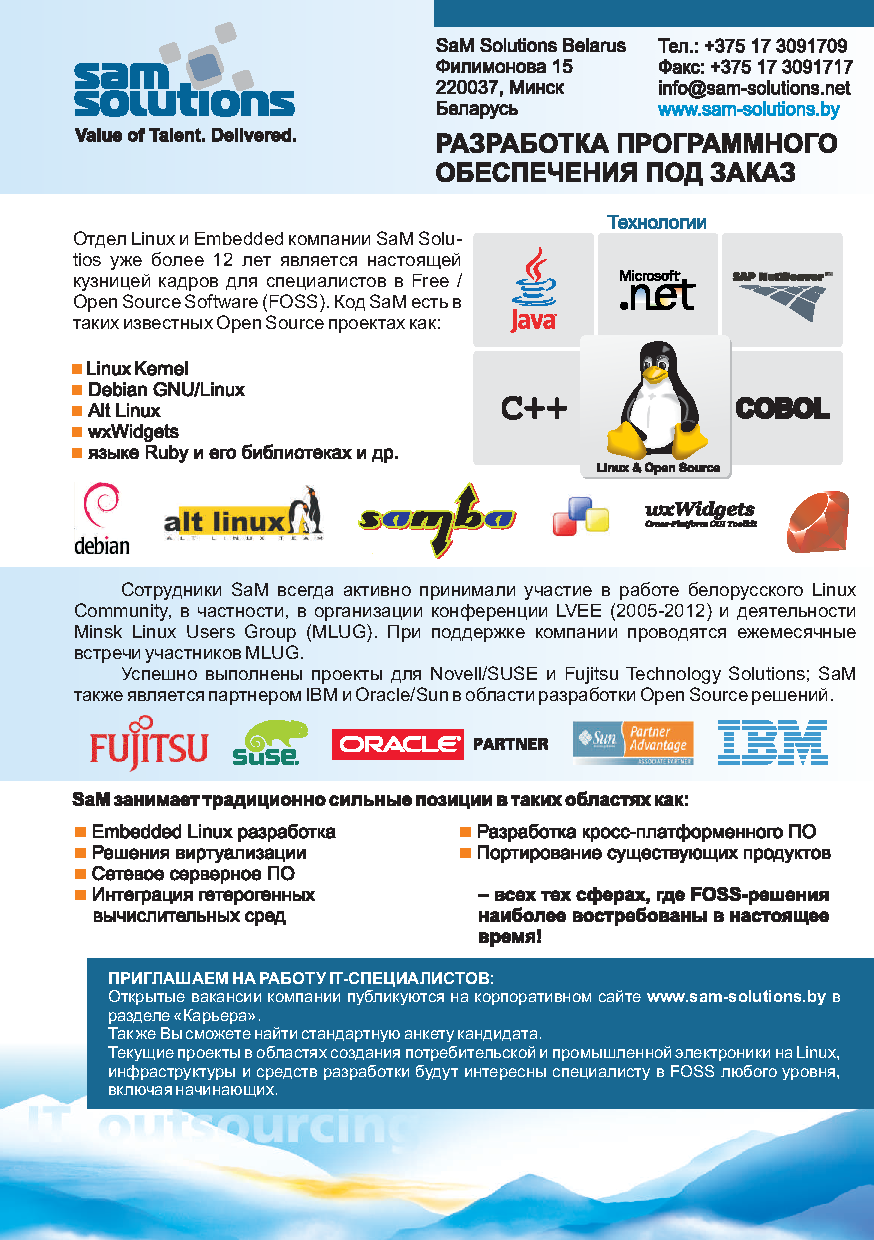
\includegraphics[height=11.8cm]{48_spons_sams.pdf}
\end{figure}
\end{document}



\documentclass[10pt, a5paper]{article}
\usepackage{pdfpages}
\usepackage{parallel}
\usepackage[T2A]{fontenc}
\usepackage{ucs}
\usepackage[utf8x]{inputenc}
\usepackage[polish,english,russian]{babel}
\usepackage{hyperref}
\usepackage{rotating}
\usepackage[inner=2cm,top=1.8cm,outer=2cm,bottom=2.3cm,nohead]{geometry}
\usepackage{listings}
\usepackage{graphicx}
\usepackage{wrapfig}
\usepackage{longtable}
\usepackage{indentfirst}
\usepackage{array}
\newcolumntype{P}[1]{>{\raggedright\arraybackslash}p{#1}}
\frenchspacing
\usepackage{fixltx2e} %text sub- and superscripts
\usepackage{icomma} % коскі ў матэматычным рэжыме
\PreloadUnicodePage{4}

\newcommand{\longpage}{\enlargethispage{\baselineskip}}
\newcommand{\shortpage}{\enlargethispage{-\baselineskip}}

\def\switchlang#1{\expandafter\csname switchlang#1\endcsname}
\def\switchlangbe{
\let\saverefname=\refname%
\def\refname{Літаратура}%
\def\figurename{Іл.}%
}
\def\switchlangen{
\let\saverefname=\refname%
\def\refname{References}%
\def\figurename{Fig.}%
}
\def\switchlangru{
\let\saverefname=\refname%
\let\savefigurename=\figurename%
\def\refname{Литература}%
\def\figurename{Рис.}%
}

\hyphenation{admi-ni-stra-tive}
\hyphenation{ex-pe-ri-ence}
\hyphenation{fle-xi-bi-li-ty}
\hyphenation{Py-thon}
\hyphenation{ma-the-ma-ti-cal}
\hyphenation{re-ported}
\hyphenation{imp-le-menta-tions}
\hyphenation{pro-vides}
\hyphenation{en-gi-neering}
\hyphenation{com-pa-ti-bi-li-ty}
\hyphenation{im-pos-sible}
\hyphenation{desk-top}
\hyphenation{elec-tro-nic}
\hyphenation{com-pa-ny}
\hyphenation{de-ve-lop-ment}
\hyphenation{de-ve-loping}
\hyphenation{de-ve-lop}
\hyphenation{da-ta-ba-se}
\hyphenation{plat-forms}
\hyphenation{or-ga-ni-za-tion}
\hyphenation{pro-gramming}
\hyphenation{in-stru-ments}
\hyphenation{Li-nux}
\hyphenation{sour-ce}
\hyphenation{en-vi-ron-ment}
\hyphenation{Te-le-pathy}
\hyphenation{Li-nux-ov-ka}
\hyphenation{Open-BSD}
\hyphenation{Free-BSD}
\hyphenation{men-ti-on-ed}
\hyphenation{app-li-ca-tion}

\def\progref!#1!{\texttt{#1}}
\renewcommand{\arraystretch}{2} %Іначай формулы ў матрыцы зліпаюцца з лініямі
\usepackage{array}

\def\interview #1 (#2), #3, #4, #5\par{

\section[#1, #3, #4]{#1 -- #3, #4}
\def\qname{LVEE}
\def\aname{#1}
\def\q ##1\par{{\noindent \bf \qname: ##1 }\par}
\def\a{{\noindent \bf \aname: } \def\qname{L}\def\aname{#2}}
}

\def\interview* #1 (#2), #3, #4, #5\par{

\section*{#1\\{\small\rm #3, #4. #5}}

\def\qname{LVEE}
\def\aname{#1}
\def\q ##1\par{{\noindent \bf \qname: ##1 }\par}
\def\a{{\noindent \bf \aname: } \def\qname{L}\def\aname{#2}}
}

%\frenchspacing
\begin{document}
\title{Голос спонсора: ITS Partner}
%\author{}
\date{}
\maketitle

~

\newpage

~

\end{document}

%\documentclass[10pt, a5paper]{article}
\usepackage{pdfpages}
\usepackage{parallel}
\usepackage[T2A]{fontenc}
\usepackage{ucs}
\usepackage[utf8x]{inputenc}
\usepackage[polish,english,russian]{babel}
\usepackage{hyperref}
\usepackage{rotating}
\usepackage[inner=2cm,top=1.8cm,outer=2cm,bottom=2.3cm,nohead]{geometry}
\usepackage{listings}
\usepackage{graphicx}
\usepackage{wrapfig}
\usepackage{longtable}
\usepackage{indentfirst}
\usepackage{array}
\newcolumntype{P}[1]{>{\raggedright\arraybackslash}p{#1}}
\frenchspacing
\usepackage{fixltx2e} %text sub- and superscripts
\usepackage{icomma} % коскі ў матэматычным рэжыме
\PreloadUnicodePage{4}

\newcommand{\longpage}{\enlargethispage{\baselineskip}}
\newcommand{\shortpage}{\enlargethispage{-\baselineskip}}

\def\switchlang#1{\expandafter\csname switchlang#1\endcsname}
\def\switchlangbe{
\let\saverefname=\refname%
\def\refname{Літаратура}%
\def\figurename{Іл.}%
}
\def\switchlangen{
\let\saverefname=\refname%
\def\refname{References}%
\def\figurename{Fig.}%
}
\def\switchlangru{
\let\saverefname=\refname%
\let\savefigurename=\figurename%
\def\refname{Литература}%
\def\figurename{Рис.}%
}

\hyphenation{admi-ni-stra-tive}
\hyphenation{ex-pe-ri-ence}
\hyphenation{fle-xi-bi-li-ty}
\hyphenation{Py-thon}
\hyphenation{ma-the-ma-ti-cal}
\hyphenation{re-ported}
\hyphenation{imp-le-menta-tions}
\hyphenation{pro-vides}
\hyphenation{en-gi-neering}
\hyphenation{com-pa-ti-bi-li-ty}
\hyphenation{im-pos-sible}
\hyphenation{desk-top}
\hyphenation{elec-tro-nic}
\hyphenation{com-pa-ny}
\hyphenation{de-ve-lop-ment}
\hyphenation{de-ve-loping}
\hyphenation{de-ve-lop}
\hyphenation{da-ta-ba-se}
\hyphenation{plat-forms}
\hyphenation{or-ga-ni-za-tion}
\hyphenation{pro-gramming}
\hyphenation{in-stru-ments}
\hyphenation{Li-nux}
\hyphenation{sour-ce}
\hyphenation{en-vi-ron-ment}
\hyphenation{Te-le-pathy}
\hyphenation{Li-nux-ov-ka}
\hyphenation{Open-BSD}
\hyphenation{Free-BSD}
\hyphenation{men-ti-on-ed}
\hyphenation{app-li-ca-tion}

\def\progref!#1!{\texttt{#1}}
\renewcommand{\arraystretch}{2} %Іначай формулы ў матрыцы зліпаюцца з лініямі
\usepackage{array}

\def\interview #1 (#2), #3, #4, #5\par{

\section[#1, #3, #4]{#1 -- #3, #4}
\def\qname{LVEE}
\def\aname{#1}
\def\q ##1\par{{\noindent \bf \qname: ##1 }\par}
\def\a{{\noindent \bf \aname: } \def\qname{L}\def\aname{#2}}
}

\def\interview* #1 (#2), #3, #4, #5\par{

\section*{#1\\{\small\rm #3, #4. #5}}

\def\qname{LVEE}
\def\aname{#1}
\def\q ##1\par{{\noindent \bf \qname: ##1 }\par}
\def\a{{\noindent \bf \aname: } \def\qname{L}\def\aname{#2}}
}

\begin{document}
\title{Интервью с участниками}
%\author{}
\date{}
\maketitle

По традиции в сборник материалов входят интервью, в которых активные участники сообщества open source делятся своим мнением о свободном ПО, открытых технологиях, роли и месте GNU/Linux, рассказывают, как видят проблематику свободных проектов. В этот раз мы решили расспросить трёх участников конференции, какое-то время назад перебравшихся из Беларуси на территорию Европейского Союза.

\section[Александр Боковой "--- principal software engineer, Red Hat, Эспоо, Финляндия]{Александр Боковой "--- principal software\linebreak engineer, Red Hat, Эспоо, Финляндия}
%\begin{figure}[ht]
%\centering{\includegraphics[width=4cm]{49_spons_altoros.jpg}}
%\end{figure}

{\noindent \bf LVEE: Традиционно первый вопрос "--- как ты познакомился с открытым ПО?}

{\noindent \bf Александр Боковой:} В 1995 году. Я учился на третьем курсе БГПУ им. Максима Танка, и одна из курсовых
работ была посвящена фрактальной геометрии. Необходимо было написать
приложение, которое бы отрисовывало и в интерактивном режиме позволяло бы
исследовать множества Жюлиа для соответствующих точек из множества
Мандельброта. 

{\noindent \bf L: Звучит очень наукоёмко\ldots}

{\noindent \bf А:} Программу я писал на Паскале, и в какой"=то момент стало не хватать
стандартной памяти в 16"=битном режиме.

{\noindent \bf L: Под MS DOS.} 

{\noindent \bf А:}  Да. Вариантов использования 32"=битного
режима было немного, поскольку требовалось еще и приличный интерфейс
пользователя обеспечить. Значит, нужна была не только графическая библиотека,
но и виджеты, обработка клавиатуры и так далее. И я нашел такую библиотеку "--- SWORD,
написанную французом Эриком Николя на C++ и поставлявшуюся вместе с DJGPP.

{\noindent \bf L: А DJGPP "--- это\ldots}

{\noindent \bf А:}  DJGPP "--- это первый порт программ проекта GNU на
платформу Intel x86, сделанный еще в 1989 году DJ Delorie. Ричард Столлман
выступал на встрече Northern England Unix Users Group в компании Data General,
где работал тогда DJ Delorie, и на вопрос о переносе GCC под MS DOS, ответил,
что это невозможно, поскольку gcc слишком большая программа, а MS-DOS работает
в 16"=битном режиме. DJ понял, что это вызов, и принял его. Так что в 1990 мы
уже имели компиляторы GNU, Emacs, binutils и много разных библиотек, все под
MS DOS в 32"=битном режиме "--- DJ пришлось написать свой DOS Extender для
того, чтобы компилировать gcc под MS DOS.

{\noindent \bf L: Как скоро ты осознал, что это вот "--- свободное ПО, сообщество, коллективная разработка?}

{\noindent \bf A:} Практически сразу. DJGPP поставлялся со всеми исходными текстами, в документации было
написано, где можно задавать вопросы. Я подписался на рассылки и первое время просто читал "--- и переписку,
где люди отвечали не только на вопросы об использовании тех или иных компонент системы, но и обсуждали бытовые
темы. Выглядело все это очень по"=домашнему, а если кто"=то предлагал патчи, то это предполагало прежде всего
устранение необходимости патчить то же самое место в следующей версии "--- rsync еще не был написан (он появился
только в 1996), а DJGPP распространялся по FTP. На наших узких линиях (64Кбит/с на весь университет) тогда
приходилось прежде всего думать, а потом делать.

{\noindent \bf L: Итак, ты использовал DJGP. А каким образом пользователь СПО стал его разработчиком?}

{\noindent \bf A:} Со SWORD и DJGPP я и начал. В 1996 вышла вторая версия DJGPP, независящая от
коммерческих компонент для своей пересборки. Главное, что случилось с DJGPP в
1994--96 годах "--- это взрывной рост популярности, привлекший огромное число
терпеливых и общительных людей в списки рассылки. Можно было задавать вопросы и
получать ответы на них, вне зависимости от того, насколько плох был твой
английский язык. В 1995 году сделали зеркало в рассылку в виде группы USENET
\url{comp.os.msdos.djgpp}, она стала доступна на локальном NNTP"=сервере университета.

{\noindent \bf L: Не помнишь, как вообще оформилась мысль: а сделаю"=ка я публичный патч? Или это получилось как"=то незаметно: пообсуждал, поисправлял "--- и вдруг люди уже пользуются?}

{\noindent \bf A:} Непубличные патчи поддерживать было неудобно, поскольку сам комплект
DJGPP распространялся в виде архивов. Так что старался отправлять исправления сразу.
К тому же, библиотеки были мне нужны для работы, но не являлись главным ее содержимым.
Лицензия SWORD "--- GNU General Public License, которую я уже читал и видел в применении
к остальным компонентам GNU. 

В 1998 я вместе с Эриком работал над третьей версией SWORD. Эта работа привела
к тому, что через несколько лет я ушел из аспирантуры, так и не закончив свою
работу над диссертацией, потому что вместо работы над методикой преподавания
фрактальной геометрии сосредоточился над SWORD "--- нужда в нормальной
интерфейсной библиотеке, работающей под MS DOS и GNU/Linux на тот момент еще не
отпала, поскольку Qt до 2000 года выходила под неудачной с точки зрения свободного ПО и написания
GPL"=программ лицензией и не поддерживала MS DOS.

Правда, после ухода из аспирантуры я сосредоточился на сетевых файловых системах,
а Эрик переписал SWORD с нуля с учетом прогресса в Qt и проект был перезапущен в 2005: 
\url{http://www.erik-n.net/software/sword/}. 

На GNU/Linux я перешел где"=то в 1996--1997, практически сразу, как появился
собственный компьютер.

{\noindent \bf L: На какой дистрибутив?}

{\noindent \bf A:} Начал со Slackware. А в декабре 1999 перевел на белорусский язык программу установки Mandrake Linux. Она вошла в Mandrake Linux Russian Edition, а потом и в основной Mandrake Linux.

Другой проект, который <<втянул>> меня в себя в приблизительно то же время, это
Midgard, система ведения веб"=сайтов. Изначально придуманная финнами Генри
Бергиусом и Юккой Зиттингом для сайта своего реконструкторского общества в
1998, система переросла викингов и стала довольно успешно использоваться как
конструктор различных сайтов, в том числе и для интранетов. Я выступал с докладом
о Midgard на первом FOSDEM в 2001 году, а в середине 2000"=х даже интегрировал
Midgard и Samba для того, чтобы обеспечить прозрачную авторизацию в
интранет"=приложениях на Midgard в среде Active Directory.

{\noindent \bf L: И тут мы наконец подобрались к твоему участию в проекте Samba. }

{\noindent \bf A:} Получается забавная ситуация: практически все проекты, над которыми я работал и
работаю, в той или иной мере связаны между собой. В 2001--2004 годах мы с Игорем
Вергейчиком работали над системой хранения, где требовалась поддержка различных
сетевых файловых систем, и я столкнулся с необходимостью внести какие"=то
изменения в Samba.  Мы написали ряд патчей, отправили их в рассылку, часть из
них приняли, часть "--- нет.  Потом Игорь доработал Samba до поддержки Unicode.
Потом я написал поддержку множественных модулей виртуальной файловой системы. И в
2003 меня пригласили в Samba Team. Принцип был простой: мой код практически
не требовал дополнительных доработок, поэтому мне дали прямой доступ к
изменению исходного текста.

Когда в декабре 2003 мы получили заказ на разработку поддержки Active Directory
в нашей системе хранения, Эндрю Триджелл, создатель Samba, просто сказал нам:
<<Зачем пытаться добавить патчи в версию 2.0, лучше помогите мне закончить 3.0,
где я уже много добился>>. То есть, взгляды апстрима и даунстрима совпали,
получилось сделать многое. Конечно, не в тот срок, который обещал Эндрю, но в
2005 у нас был вполне работающий продукт.

{\noindent \bf L: Какие различия бросаются в глаза, если сравнивать опенсорс"=комьюнити в СНГ с англоязычным? }

{\noindent \bf А:} Если тебе нужны какие-то изменения к существующему коду, ты их пишешь,
оформляешь патчи, отправляешь в рассылку и обсуждаешь с другими разработчиками.
Патчи могут принять сразу, могут не принять совсем, но чаще всего приходится
объяснять и находить компромисс. Работа над отдельными изменениями может
затянуться на годы. В СНГ есть разработчики свободного ПО (и их много), но
очень мало сообществ разработчиков свободного ПО как таковых. Те, кто
заинтересован, участвуют в международных проектах различного масштаба. Новые
проекты с преимущественно русскоязычным общением -- редкость, они мало кому из
разработчиков нужны. Они, безусловно, нужны пользователям, но сколько времени
разработчики могут посвятить локальным пользователям?

С другой стороны, уровень знания английского языка может препятствовать
активному участию в существующих проектах, даже если кто"=то готов написать
код, часто сталкиваешься с тем, что довести работу до конца они не могут "---
нужна документация на английском, участие в дискуссиях, причем в темпе
активности конкретного проекта, а не разработчика.  В этом смысле разница в
Европе особенно бросается в глаза, здесь проблем с английским языком среди
разработчиков свободного ПО нет, даже в традиционно неанглоязычных странах.
Английский "--- lingua franca свободного ПО.

Другой аспект взаимодействия в проектах свободного ПО, это значительно меньший
накал страстей в рассылках по сравнению с тем, что я вижу в русскоязычной
среде. 

{\noindent \bf L: О да! В этом сезоне организаторская рассылка LVEE переживала 
как раз такую драму :) }

{\noindent \bf А:} Наблюдается заметное ослабление эмоций при общении с пользователями при
продвижении с востока на запад в Европе "--- если, скажем, польские пользователи
еще пишут с активным выражением своей позиции в отношении разработчиков на IRC"=каналах, 
то там, где преобладают английские или американские пользователи,
атмосфера менее накалена. В программном обеспечении есть и будут ошибки, никто
не идеален, поэтому поиск источника ошибки "--- рабочая ситуация, не требующая
перехода на личности. Почему"=то русскоязычное пространство переполнено полярным
выражением собственных эмоций.

{\noindent \bf L: Кстати, возвращаясь к теме работы над продуктами. Как бы ты охарактеризовал свой личный опыт использования СПО в корпоративном секторе?}

{\noindent \bf A:} Мне повезло, я последние лет пятнадцать использую свободное ПО в рабочем окружении. В
последние пять"=семь лет с этим стало совсем хорошо из"=за активного продвижения
мобильных платформ и веб"=приложений, которые вынесли из многих компаний
специализированные плагины и прочие платформо"=зависимые клиентские компоненты.

Работа над Samba и FreeIPA предполагает, что приходится иметь дело с
проприетарной инфраструктурой и клиентским ПО, но для обеспечения собственной
жизни в корпоративной среде мне они практически не нужны. Гораздо сложнее
с проприетарным ПО на серверной стороне "--- даже если интерфейс к нему позволяет
использовать свободное ПО на клиентской стороне, доступность данных в
большинстве таких систем завязана на производителя. Это данных наших компаний,
но извлечь их в структурированном виде и перенести куда"=то еще мы часто просто
не можем.

{\noindent \bf L: Последний вопрос, о Redhat. Как это выглядит изнутри?}

{\noindent \bf А:} По"=домашнему. В прямом смысле "--- большую часть времени
я работаю из дома. У нас небольшой офис в Эспоо, рабочее место у меня есть, но
появляюсь я в офисе нечасто, поскольку моя команда разбросана по миру. Из инструментов
общения "--- электронная почта, IRC, интернет"=телефония и видео"=конференции.
Раз или два в год получается встретиться лично, это время используется для интенсивных
дискуссий, особенно в феврале, когда в Брно (Чехия) проходит традиционная конференция
\url{devconf.cz} "--- на нее съезжаются ребята из многих команд и есть шанс обсудить
предстоящие задачи на год вперед с теми, с кем не получается пересекаться <<в эфире>>
из"=за часовых поясов.

Самым удивительным для меня четыре года назад было то, как мало информации скрыто от
посторонних глаз. Если Red Hat участвует в разработке какого"=то проекта, то вся информация
доступна на сайте апстрима. Внутри только детали планов интеграции конкретных апстримных
версий в продукты компании, а весь дизайн новых функций и их разработка ведутся публично.

А моя история, кстати, замкнулась: DJ Delorie работает в Red Hat и обеспечивает нас
работающими компиляторами вот уже более шестнадцати лет.


\section[Андрей Шадура "--- software engineer, Collabora, Братислава, Словакия]{Андрей Шадура "--- software engineer, \linebreak Collabora, Братислава, Словакия}

%\begin{figure}[ht]
%\centering{\includegraphics[width=4cm]{49_spons_altoros.jpg}}
%\end{figure}

{\noindent \bf Андрей Шадура:} Моё знакомство со свободным ПО произошло, когда я в школьные времена ещё пользовался DOS и Windows и программировал для них на турбопаскале. Некоторые библиотеки, которыми я пользовался, поставлялись в бинарном виде и без исходных кодов, некоторые были с исходниками и README о том, что коммерческое использование запрещено, а к некоторым прилагался объёмный файл COPYING с текстом лицензии. Примерно в то же время я узнал об альтернативных операционных системах из тогдашних компьютерных журналов, и идея того, что ОС можно «похачить» изнутри меня очень заинтересовала. Позднее я скачал несколько однодискетных дистрибутивов (кроме как по dial"=up, мне Интернет был слабодоступен) и поиграл с ними, но «настоящий» Linux я не попробовал до учёбы в университете.

{\noindent \bf L: И какие были впечатления от этого самого первого опыта, от Unix"=подобных систем?}

{\noindent \bf А:} Как раз первый из этих однодисковых дистрибутивов и был сертифицированный Unix "--- демо"=версия QNX. Было конечно интересно увидеть что-то совсем другое, и там был такой GUI! Но возможности у этой версии были сильно ограниченными. Затем был очередной однодискетный Linux-дистрибутив, Trinux. Я о нём где"=то прочитал, не то в <<Компьютерной газете>>, не то в <<Хакере>>\ldots

{\noindent \bf L: Эксперимент прошёл с тем же примерно успехом?}

{\noindent \bf А:} Да. А затем меня увлекло местное движение <<даунгрейдеров>>, и я провел несколько лет в окружении FreeDOS, GEM, ViewMAX, других древних систем и их опенсорсных реинкарнаций. Но, кстати, в DOS меня буквально бесили все тамошние недокументированные функции.

{\noindent \bf L: Ты имеешь в виду тамошний зоопарк системных вызовов? Все эти int 21h?}

{\noindent \bf А:} Да. Ещё в школьные годы я часами в библиотеке просиживал, выуживая прерывания и номера функций из старой литературы и новых журналов. В сравнении с этим, а также недокументированными функциями Windows, жизнь в Linux "--- просто раздолье.

{\noindent \bf L: Итак, следующий этап "--- уже в университете?}

{\noindent \bf А:} Это был уже  2005 год, там я получил от Дениса Пынькина, который уже был ALT Linux developer, копию ALT Linux 2.2 Master. Это, кстати, было в преддверии выхода версии 2.4, и он меня уговаривал подождать, но мне хотелось здесь и сейчас, и я на следующий же день проинсталлировал 2.2. Получилось без звука, были проблемы с X"=сервером (конечно, без всякого опыта), и это конечно было круто "--- иметь действующую Linux-систему, но основной ОС она в тот раз для меня не стала.

{\noindent \bf L: А когда наконец стала?}

{\noindent \bf А:} Годом позже. Работал в лаборатории института ядерных проблем, я получил аккаунт на сервере под управлением Debian <<sarge>>, попросил "--- и мне сделали бутстрап этой инсталляции на мой жёсткий диск. Потом эта машина у меня дома занималась маршрутизацией, пока в 2009 году не заменил ее маленьким роутером на MIPS. Ну а через несколько месяцев общения с этой машиной Debian стал и моей десктоп"=системой. И тогда же захотелось как"=то контрибутить в проект. Сначала начал делать патчи и баг"=репорты к тому, чем пользовался. А в 2009 запакетировал первое приложение.

{\noindent \bf L: Что это было?}

{\noindent \bf А:} Случайное, практически на спор. Кто"=то  пожаловался, что это очень тяжело "--- делать пакеты для Debian, я ответил, что нет ничего проще, и услышал в ответ: <<Ну давай, запакетируй мой проект, посмотрим, сколько это у тебя займёт времени>>. И за пару часов подготовил пакет для gdigi.

А потом, уже на LVEE, Дмитрий Бородаенко (в то время "--- единственный Debian Developer из Беларуси) побудил меня на больший вклад. Первый пакет, который я по"=настоящему мэйнтэнил, был tclxml.

Позже, в 2010, занялся исправлением некоторых багов ifupdown, инструмента конфигурирования сети в Debian, ну и так далее.

{\noindent \bf L: Ты принципиальный Debian'щик?}

{\noindent \bf А:} Конечно, не только Debian. Я вообще вношу вклад время от времени в разные свободные проекты, да и свои собственные есть.
Кроме того, время от времени вношу правки в википедию, а еще, достаточно регулярно "--- в OpenStreetMap.

{\noindent \bf L: Теперь "--- к переезду. Скажи, отъезд из Беларуси как"=нибудь повлиял на твои взаимоотношения с миром свободного ПО?}

{\noindent \bf А:} В некотором смысле повлиял: проще, ближе и быстрее стало ездить на всевозможные конференции и прочие спринты и hackweeks. Из событий, на которых я побывал недавно: LinuxDays.cz в Праге (три раза), FOSDEM (два раза), Cambridge Debian Miniconf\ldots Ну и недавняя hack week в Копенгагене.

{\noindent \bf L: Неполиткорректные соотечественники должны в этот момент воскликнуть <<дорвался>> :)}

{\noindent \bf А:} Ага, так и есть. Но вообще, с кругом общения сложнее. Чтобы было понятнее, я за чуть более, чем три года в Словакии переезжал два раза. Первое время здесь я жил в деревне, с кругом было вообще никак.

Но я активно этот круг искал в других местах. Например, познакомился с местным сообществом OpenStreetMap (Freemap.sk) и через две недели после переезда поехал с ними на mapping party. Общаться было сложновато, потому как по"=английски я хоть и говорю, но мне хотелось научиться говорить по"=словацки, а знания были очень слабы. А по"=белорусски меня понимали слабо :)

{\noindent \bf L: Все эти переезды были связаны с работой?}

{\noindent \bf А:} Да, одна закончилась, новая находилась в другом месте. Через год, кстати, я приехал на университетскую конференцию OSSConf в Жилине, о которой узнал случайно, и познакомился там с кучей сторонников free software.

Да, еще забыл. Через пару месяцев после mapping party в результате активных поисков я узнал, что в Братиславе есть хакерспейс Progressbar, и направился туда на одно из мероприятий. мероприятий там вообще много проводилось, собирались какие-то питонисты, опенстритмапперы и прочие, но поездка туда занимала бы 5 часов в одну сторону, поэтому часто посещать их не получалось, пока я не переехал в конечном итоге в Братиславу.

{\noindent \bf L: Вопрос по поводу членов опенсорс"=комьюнити: какие-то отличия после переезда? Бросалась в глаза какая"=то разница?}

{\noindent \bf А:} С одной стороны, здесь я заметил, что линуксами, в основном Ubuntu, пользуются иногда люди, далекие от IT вообще. И это меня удивило.

{\noindent \bf L: Ну да, у нас это обычно члены семей линуксоидов.}

{\noindent \bf А:} Из примеров вспоминается одна знакомая, которая мне рассказывала о том, какая замечательная Ubuntu и какой ужасный Debian. При этом она ни разу в жизни, как мне кажется, не видела командную строку ни одного, ни другого. Её работа вообще связана с образовательными программами\ldots

{\noindent \bf L: Ты говоришь, что это с одной стороны. А с другой?}

{\noindent \bf А:} С другой стороны, пассивность «активистов». В Жилине, где я жил, есть некоторое количество людей, пользующихся Linux и знающих про свободное ПО (часть из них работает в местном университете). И за целый год проводится одно, максимум два события на тему: тот самый OSSConf, и иногда OSS Weekend. Это при том, что в городе вроде как третий по величине технический университет страны\ldots 

Ну да ладно, Жилина, маленький городок. Берем Братиславу. Здесь есть STU, Словацкий технический университет, здесь есть Progressbar.  Progressbar организует небольшие митапы иногда, но нерегулярно. Я предлагал создать регулярные встречи, подобие минских линуксовок. Никто энтузиазма не проявил, но один человек рассказал, что он когда"=то пробовал делать какие"=то встречи, но всё угасло.

Подобный вопрос я поднял на OSS Weekend, который в прошлом году (и в этом тоже) проводился в Братиславе. <<Надо бы\ldots>> был ответ :)

Но, с третьей стороны, как ни странно, местное Ruby"=сообщество достаточно активное. Встречи проводят несколько раз в месяц, называются Рубислава.


\section[Евгений Калюта "--- experienced developer, Ericsson, Хельсинки, Финляндия]{Евгений Калюта "--- experienced develo\-per, Ericsson, Хельсинки, Финляндия}

%\begin{figure}[ht]
%\centering{\includegraphics[width=4cm]{49_spons_altoros.jpg}}
%\end{figure}

{\noindent \bf L: Традиционный первый вопрос "--- твое первое знакомство с открытым ПО. Может быть первые впечатления, если они были?}

{\noindent \bf Евгений Калюта:} Я расскажу долгую историю :) 

{\noindent \bf L: Отлично :)}

{\noindent \bf Е:} Я из провинции. Доступность как информации, так и техники тогда была не на высоте. Учитель информатики у нас был молодой, активный, сразу после
института. Это был 7"=ой класс, когда нам поставили <<Корветы>>. 

{\noindent \bf L: Действительно, издалека :)}


{\noindent \bf Е:} Программы обучения толком не было, нас в класс пускали, но директор строго говорила
<<седьмому классу только игры>>. Однако учитель некоторым пытливым показал книжки по Basic и давал основы алгоритмизации (в моём классе нас таких пытливых было двое). Он же (учитель) как"=то рассказал, что для настоящего
программирования бывает ассемблер (что это я тогда представлял с трудом), и C.

{\noindent \bf L: Этого хотелось?}

{\noindent \bf Е:} Этого очень хотелось. Но книг в доступности не было (начало девяностых).

Однажды в книжном я таки увидел какую"=то брошюрку, то ли про C, то ли про что"=то ещё, но главное, что в предисловии было замечено, что вот такой вот он язык C, и на нём написали Unix, на котором работает Интернет.

Очень захотелось как C, так и Unix. При мысли о них в душе возникал некий трепет.

Заработать на первый PC мне удалось кажется на третьем курсе. Где"=то в это
время, кажется в <<Компьютерной газете>>, пробежала статья с заголовком <<Попробуйте Linux>>. Это был Unix, этого хотелось. Плюс мысль о том, что
можно посмотреть в исходный код настоящего ядра настоящей операционной
системы, вызывала ощущения на грани\ldots.

{\noindent \bf L: Напишем, что мысль вызывала катарсис.}

{\noindent \bf Е:} Хорошо :) Но этого негде было взять (из моего круга общения, ясное дело, который на
тот момент охватывал не очень много людей, приобщённых к IT). Первый диск, привезённый одной компьютерной фирмочкой, нёс на себе две безнадёжно испорченные версии дистрибутива <<Caldera>>, ни одна из них не могла поставиться
по объективным причинам.

{\noindent \bf L: Из"=за неумелой перепаковки?}

Ну как, если правильно подмонтировать распакованный tar.gz
одиного из них как umsdos, то может шансы и были бы, но я тогда я не имел
об этом ни малейшего представления. Я потрогал консоль инсталлятора,
смог даже перенести файл на ДОС"=раздел, испытал\ldots катарсис, понятное
дело, ну и как бы на этом всё.

{\noindent \bf L: А твой первый работающий Linux?}

{\noindent \bf Е:} Первым работающим оказался русский клон Redhat 4.2 "--- он назывался <<Красная шапочка
5.0>>, он умел ставиться, он умел грузиться, на нём собиралось ядро и, если
мне не изменяет память, KDE 1.0 (к тому моменту у меня уже были контакты,
у кого это можно было взять).

Подытоживая, пришёл к открытому ПО я случайно (я о нём ничего не знал) из
желания приобщиться к великому, к Unix, и (за неимением)  других вариантов не искал.

{\noindent \bf L: Несколько слов про твой путь из пользователей свободного ПО в разработчики?}

{\noindent \bf Е:} Ну, вообще контрибуций у меня не очень много. В детстве я был <<хорошим
советским мальчиком>> и очень боялся публичного порицания. Поэтому долгое
время в <<серьёзные>> проекты было лезть страшновато\ldots Что очень зря. С
большего, по отношению к открытым проектам, это прошло только пару лет
назад. А с Debian в период большого желания просто случился неприятный
казус, который затормозил мой путь в Debian Developer.



{\noindent \bf L: У нас в этом году снова тематическое интервью. Поэтому еще группа вопросов, инспирированная отъездом интервьюируемого из Беларуси. Какие различия бросаются в глаза, если сравнивать опенсорс-комьюнити в
СНГ с англоязычным? Европейских и белорусских (и вообще русскоязычных, наверное) разработчиков?}

{\noindent \bf Е:} Про англоязычные комьюнити особенно говорить бессмысленно, ибо белорусы "--- такие же полноправные участники этого коммунити. Сами и всё видят, и несут вклад в общую атмосферу.

{\noindent \bf L: Ну, речь скорее о локальных комьюнити. }

{\noindent \bf Е:} Локального, про Финляндию могу сказать чуть личного.

{\noindent \bf L: Очень хорошо. }

{\noindent \bf Е:} Я бы отметил, что различные открытые проекты тут занимают видимую часть 
общественной жизни "--- тут вообще модны всевозможные общественные обсуждения и
инициативы). Участие студентов в opensource очень естественно: помню, поразился количеством Debian Developers.  

{\noindent \bf L: Если подумать, не только Debian "--- в конце концов, происхождение Linux как такового\ldots}

{\noindent \bf Е:} Финляндия дала миру open source кроме ядра Linux и некоторые менее известные вещи, такие как протокол IRC, клиент  irssi, оконный менеджер ion (славящийся своим проблемным автором), протокол ssh, почтовый сервер dovecot "--- это навскидку.

Местные заинтересованные вполне чувствуют себя частью мирового движения, активно участвуют в проектах, конференциях, инициативах по всему миру, устраивают их у себя. Первый мой debconf был в Финляндии, пару раз был на
дебиановских bug\linebreak squashing party, они тоже как правило не совсем локальные. Можно, наверное, сказать, что открытости в сообществе порядочно поболе. 


А еще для пущего приобщения студентам в плюс к традиционным конференциям устраивают различного рода встречи и круглые столы с известными в мире open source людьми, и они как правило не ограничиваются студентами. Я был на лекциях Столлмана и Торвальдса (на той самой, про Nvidia).

И потом, обсуждать вопросы с местными ребятами мне лично очень приятно "--- это, как правило, спокойно, по делу, без излишнего давления.

В общем, все это очень повлияло и на личную систему <<свой "--- чужой>>. Она слабо коррелирует с границами и языками.

Кроме того, на момент переезда (2006 год), проникновения IT в общественную жизнь было порядочно больше, чем в Беларуси, поэтому и восприятие околоайтишных движений более серьёзно.

В остальном точно так же: лобби коммерческих компаний имеет больший вес. Слышал истории об оспаривании некоторых государственных тендеров, на что банально не хватило денег.

{\noindent \bf L: Еще интересный вопрос "--- твой личный опыт использования СПО в корпоративном секторе. Понятно, всегда есть работодатель\ldots}

{\noindent \bf Е:} Используется активно, там где не противоречит коммерческим интересам. Но, как мы знаем, построить коммерческую систему на базе свободного ПО и поддержки
комьюнити у Нокии не получилось. Вклад она при этом внесла очень порядочный, надо отметить.

В Эриксоне, безусловно, оно тоже используется в разных местах, и даже что"=то выползает наружу. 

{\noindent \bf L: В смысле наработок, которые отдаются сообществу?}

{\noindent \bf Е:} В целом, отдавать из корпорации назад обычно сопряжено с трудностями. Как правило, это связано с законодательством США и нежеланием рисковать, ну или и простая жадность иногда. Но есть и позитивные случаи: на память сразу приходят TIPC\footnote{\url{http://en.wikipedia.org/wiki/TIPC}} и \linebreak Eclipse.

А если про компании вообще, уже не из личного опыта "--- понятно, раньше Nokia и окружающие её компании задавали тон, но и сейчас тут присутствует некоторое количество компаний, серьёзно вкладывающих в разработку открытых проектов: это небольшой (по их меркам, в несколько сотен) офис OTC Intel, это наверное наиболее <<честный>> контрибьютор, но есть Huawei, Samsung, (члены Linaro), Nvidia опять же. В определённом смысле присутствуют Red Нat и TI.

\end{document}



\newpage

\makeatletter
\let\enddocument\@lvee@enddoc
\let\input\@lvee@input
\makeatother

\eof


